\documentclass[twoside]{book}

% Packages required by doxygen
\usepackage{fixltx2e}
\usepackage{calc}
\usepackage{doxygen}
\usepackage[export]{adjustbox} % also loads graphicx
\usepackage{graphicx}
\usepackage[utf8]{inputenc}
\usepackage{makeidx}
\usepackage{multicol}
\usepackage{multirow}
\PassOptionsToPackage{warn}{textcomp}
\usepackage{textcomp}
\usepackage[nointegrals]{wasysym}
\usepackage[table]{xcolor}

% Font selection
\usepackage[T1]{fontenc}
\usepackage[scaled=.90]{helvet}
\usepackage{courier}
\usepackage{amssymb}
\usepackage{sectsty}
\renewcommand{\familydefault}{\sfdefault}
\allsectionsfont{%
  \fontseries{bc}\selectfont%
  \color{darkgray}%
}
\renewcommand{\DoxyLabelFont}{%
  \fontseries{bc}\selectfont%
  \color{darkgray}%
}
\newcommand{\+}{\discretionary{\mbox{\scriptsize$\hookleftarrow$}}{}{}}

% Page & text layout
\usepackage{geometry}
\geometry{%
  a4paper,%
  top=2.5cm,%
  bottom=2.5cm,%
  left=2.5cm,%
  right=2.5cm%
}
\tolerance=750
\hfuzz=15pt
\hbadness=750
\setlength{\emergencystretch}{15pt}
\setlength{\parindent}{0cm}
\setlength{\parskip}{3ex plus 2ex minus 2ex}
\makeatletter
\renewcommand{\paragraph}{%
  \@startsection{paragraph}{4}{0ex}{-1.0ex}{1.0ex}{%
    \normalfont\normalsize\bfseries\SS@parafont%
  }%
}
\renewcommand{\subparagraph}{%
  \@startsection{subparagraph}{5}{0ex}{-1.0ex}{1.0ex}{%
    \normalfont\normalsize\bfseries\SS@subparafont%
  }%
}
\makeatother

% Headers & footers
\usepackage{fancyhdr}
\pagestyle{fancyplain}
\fancyhead[LE]{\fancyplain{}{\bfseries\thepage}}
\fancyhead[CE]{\fancyplain{}{}}
\fancyhead[RE]{\fancyplain{}{\bfseries\leftmark}}
\fancyhead[LO]{\fancyplain{}{\bfseries\rightmark}}
\fancyhead[CO]{\fancyplain{}{}}
\fancyhead[RO]{\fancyplain{}{\bfseries\thepage}}
\fancyfoot[LE]{\fancyplain{}{}}
\fancyfoot[CE]{\fancyplain{}{}}
\fancyfoot[RE]{\fancyplain{}{\bfseries\scriptsize Generated by Doxygen }}
\fancyfoot[LO]{\fancyplain{}{\bfseries\scriptsize Generated by Doxygen }}
\fancyfoot[CO]{\fancyplain{}{}}
\fancyfoot[RO]{\fancyplain{}{}}
\renewcommand{\footrulewidth}{0.4pt}
\renewcommand{\chaptermark}[1]{%
  \markboth{#1}{}%
}
\renewcommand{\sectionmark}[1]{%
  \markright{\thesection\ #1}%
}

% Indices & bibliography
\usepackage{natbib}
\usepackage[titles]{tocloft}
\setcounter{tocdepth}{3}
\setcounter{secnumdepth}{5}
\makeindex

% Hyperlinks (required, but should be loaded last)
\usepackage{ifpdf}
\ifpdf
  \usepackage[pdftex,pagebackref=true]{hyperref}
\else
  \usepackage[ps2pdf,pagebackref=true]{hyperref}
\fi
\hypersetup{%
  colorlinks=true,%
  linkcolor=blue,%
  citecolor=blue,%
  unicode%
}

% Custom commands
\newcommand{\clearemptydoublepage}{%
  \newpage{\pagestyle{empty}\cleardoublepage}%
}

\usepackage{caption}
\captionsetup{labelsep=space,justification=centering,font={bf},singlelinecheck=off,skip=4pt,position=top}

%===== C O N T E N T S =====

\begin{document}

% Titlepage & ToC
\hypersetup{pageanchor=false,
             bookmarksnumbered=true,
             pdfencoding=unicode
            }
\pagenumbering{roman}
\begin{titlepage}
\vspace*{7cm}
\begin{center}%
{\Large M\+I\+P\+S16bits }\\
\vspace*{1cm}
{\large Generated by Doxygen 1.8.11}\\
\end{center}
\end{titlepage}
\clearemptydoublepage
\tableofcontents
\clearemptydoublepage
\pagenumbering{arabic}
\hypersetup{pageanchor=true}

%--- Begin generated contents ---
\chapter{Hierarchical Index}
\section{Class Hierarchy}
This inheritance list is sorted roughly, but not completely, alphabetically\+:\begin{DoxyCompactList}
\item \contentsline{section}{M\+I\+PS\+:\+:C\+PU}{\pageref{classMIPS_1_1CPU}}{}
\item \contentsline{section}{M\+I\+PS\+:\+:Decoder\+Finder}{\pageref{classMIPS_1_1DecoderFinder}}{}
\item \contentsline{section}{M\+I\+PS\+:\+:Encoder}{\pageref{classMIPS_1_1Encoder}}{}
\begin{DoxyCompactList}
\item \contentsline{section}{M\+I\+PS\+:\+:Format\+I\+Encoder}{\pageref{classMIPS_1_1FormatIEncoder}}{}
\item \contentsline{section}{M\+I\+PS\+:\+:Format\+I\+I\+Encoder}{\pageref{classMIPS_1_1FormatIIEncoder}}{}
\item \contentsline{section}{M\+I\+PS\+:\+:Format\+I\+I\+I\+Encoder}{\pageref{classMIPS_1_1FormatIIIEncoder}}{}
\item \contentsline{section}{M\+I\+PS\+:\+:Format\+I\+V\+Encoder}{\pageref{classMIPS_1_1FormatIVEncoder}}{}
\item \contentsline{section}{M\+I\+PS\+:\+:Format\+V\+Encoder}{\pageref{classMIPS_1_1FormatVEncoder}}{}
\item \contentsline{section}{M\+I\+PS\+:\+:Format\+V\+I\+Encoder}{\pageref{classMIPS_1_1FormatVIEncoder}}{}
\item \contentsline{section}{M\+I\+PS\+:\+:Format\+V\+I\+I\+Encoder}{\pageref{classMIPS_1_1FormatVIIEncoder}}{}
\end{DoxyCompactList}
\item \contentsline{section}{M\+I\+PS\+:\+:Encoder\+Factory}{\pageref{classMIPS_1_1EncoderFactory}}{}
\item \contentsline{section}{M\+I\+PS\+:\+:Event}{\pageref{classMIPS_1_1Event}}{}
\item \contentsline{section}{M\+I\+PS\+:\+:Event\+Dispatcher}{\pageref{classMIPS_1_1EventDispatcher}}{}
\item \contentsline{section}{M\+I\+PS\+:\+:Event\+Listener}{\pageref{classMIPS_1_1EventListener}}{}
\item \contentsline{section}{M\+I\+PS\+:\+:File\+Reader}{\pageref{classMIPS_1_1FileReader}}{}
\item \contentsline{section}{M\+I\+PS\+:\+:Filter}{\pageref{classMIPS_1_1Filter}}{}
\begin{DoxyCompactList}
\item \contentsline{section}{M\+I\+PS\+:\+:Space\+Filter}{\pageref{classMIPS_1_1SpaceFilter}}{}
\end{DoxyCompactList}
\item \contentsline{section}{M\+I\+PS\+:\+:Full\+Adder}{\pageref{classMIPS_1_1FullAdder}}{}
\item \contentsline{section}{M\+I\+PS\+:\+:Instruction}{\pageref{classMIPS_1_1Instruction}}{}
\begin{DoxyCompactList}
\item \contentsline{section}{M\+I\+PS\+:\+:InstructionI}{\pageref{classMIPS_1_1InstructionI}}{}
\begin{DoxyCompactList}
\item \contentsline{section}{M\+I\+PS\+:\+:Add\+Inc\+Instruction}{\pageref{classMIPS_1_1AddIncInstruction}}{}
\item \contentsline{section}{M\+I\+PS\+:\+:Add\+Instruction}{\pageref{classMIPS_1_1AddInstruction}}{}
\item \contentsline{section}{M\+I\+PS\+:\+:And\+Instruction}{\pageref{classMIPS_1_1AndInstruction}}{}
\item \contentsline{section}{M\+I\+PS\+:\+:Andnota\+Instruction}{\pageref{classMIPS_1_1AndnotaInstruction}}{}
\item \contentsline{section}{M\+I\+PS\+:\+:Asl\+Instruction}{\pageref{classMIPS_1_1AslInstruction}}{}
\item \contentsline{section}{M\+I\+PS\+:\+:Asr\+Instruction}{\pageref{classMIPS_1_1AsrInstruction}}{}
\item \contentsline{section}{M\+I\+PS\+:\+:Deca\+Instruction}{\pageref{classMIPS_1_1DecaInstruction}}{}
\item \contentsline{section}{M\+I\+PS\+:\+:Inca\+Instruction}{\pageref{classMIPS_1_1IncaInstruction}}{}
\item \contentsline{section}{M\+I\+PS\+:\+:Nand\+Instruction}{\pageref{classMIPS_1_1NandInstruction}}{}
\item \contentsline{section}{M\+I\+PS\+:\+:Nor\+Instruction}{\pageref{classMIPS_1_1NorInstruction}}{}
\item \contentsline{section}{M\+I\+PS\+:\+:Ones\+Instruction}{\pageref{classMIPS_1_1OnesInstruction}}{}
\item \contentsline{section}{M\+I\+PS\+:\+:Or\+Instruction}{\pageref{classMIPS_1_1OrInstruction}}{}
\item \contentsline{section}{M\+I\+PS\+:\+:Ornotb\+Instruction}{\pageref{classMIPS_1_1OrnotbInstruction}}{}
\item \contentsline{section}{M\+I\+PS\+:\+:Passa\+Instruction}{\pageref{classMIPS_1_1PassaInstruction}}{}
\item \contentsline{section}{M\+I\+PS\+:\+:Pass\+Not\+A\+Instruction}{\pageref{classMIPS_1_1PassNotAInstruction}}{}
\item \contentsline{section}{M\+I\+PS\+:\+:Subdec\+Instruction}{\pageref{classMIPS_1_1SubdecInstruction}}{}
\item \contentsline{section}{M\+I\+PS\+:\+:Sub\+Instruction}{\pageref{classMIPS_1_1SubInstruction}}{}
\item \contentsline{section}{M\+I\+PS\+:\+:Xnor\+Instruction}{\pageref{classMIPS_1_1XnorInstruction}}{}
\item \contentsline{section}{M\+I\+PS\+:\+:Xor\+Instruction}{\pageref{classMIPS_1_1XorInstruction}}{}
\item \contentsline{section}{M\+I\+PS\+:\+:Zero\+Instruction}{\pageref{classMIPS_1_1ZeroInstruction}}{}
\end{DoxyCompactList}
\item \contentsline{section}{M\+I\+PS\+:\+:Instruction\+II}{\pageref{classMIPS_1_1InstructionII}}{}
\begin{DoxyCompactList}
\item \contentsline{section}{M\+I\+PS\+:\+:Loadlit\+Instruction}{\pageref{classMIPS_1_1LoadlitInstruction}}{}
\end{DoxyCompactList}
\item \contentsline{section}{M\+I\+PS\+:\+:Instruction\+I\+II}{\pageref{classMIPS_1_1InstructionIII}}{}
\begin{DoxyCompactList}
\item \contentsline{section}{M\+I\+PS\+:\+:Lch\+Instruction}{\pageref{classMIPS_1_1LchInstruction}}{}
\item \contentsline{section}{M\+I\+PS\+:\+:Lcl\+Instruction}{\pageref{classMIPS_1_1LclInstruction}}{}
\end{DoxyCompactList}
\end{DoxyCompactList}
\item \contentsline{section}{M\+I\+PS\+:\+:Instruction\+Decoder}{\pageref{classMIPS_1_1InstructionDecoder}}{}
\begin{DoxyCompactList}
\item \contentsline{section}{M\+I\+PS\+:\+:Instruction\+I\+Decoder}{\pageref{classMIPS_1_1InstructionIDecoder}}{}
\end{DoxyCompactList}
\item \contentsline{section}{M\+I\+PS\+:\+:Interpreter}{\pageref{classMIPS_1_1Interpreter}}{}
\item \contentsline{section}{M\+I\+PS\+:\+:Label}{\pageref{structMIPS_1_1Label}}{}
\item \contentsline{section}{M\+I\+PS\+:\+:Event\+Dispatcher\+:\+:Listener\+Map}{\pageref{structMIPS_1_1EventDispatcher_1_1ListenerMap}}{}
\item \contentsline{section}{M\+I\+PS\+:\+:Queue$<$ T $>$\+:\+:Node}{\pageref{structMIPS_1_1Queue_1_1Node}}{}
\item \contentsline{section}{M\+I\+PS\+:\+:Queue$<$ T $>$}{\pageref{classMIPS_1_1Queue}}{}
\item \contentsline{section}{M\+I\+PS\+:\+:Queue$<$ M\+I\+PS\+:\+:Event\+Listener $\ast$ $>$}{\pageref{classMIPS_1_1Queue}}{}
\item \contentsline{section}{M\+I\+PS\+:\+:Register}{\pageref{classMIPS_1_1Register}}{}
\item \contentsline{section}{M\+I\+PS\+:\+:Register\+Bank}{\pageref{classMIPS_1_1RegisterBank}}{}
\item R\+Encoder\begin{DoxyCompactList}
\item \contentsline{section}{M\+I\+PS\+:\+:Add\+Instruction\+Encoder}{\pageref{classMIPS_1_1AddInstructionEncoder}}{}
\end{DoxyCompactList}
\item runtime\+\_\+error\begin{DoxyCompactList}
\item \contentsline{section}{M\+I\+PS\+:\+:Interpreter\+Exception}{\pageref{classMIPS_1_1InterpreterException}}{}
\end{DoxyCompactList}
\item \contentsline{section}{M\+I\+PS\+:\+:Signal\+Extender}{\pageref{classMIPS_1_1SignalExtender}}{}
\item \contentsline{section}{M\+I\+PS\+:\+:Signal\+Inversor}{\pageref{classMIPS_1_1SignalInversor}}{}
\item \contentsline{section}{M\+I\+PS\+:\+:Tokenizer}{\pageref{classMIPS_1_1Tokenizer}}{}
\end{DoxyCompactList}

\chapter{Class Index}
\section{Class List}
Here are the classes, structs, unions and interfaces with brief descriptions\+:\begin{DoxyCompactList}
\item\contentsline{section}{\hyperlink{classMIPS_1_1AddIncInstruction}{M\+I\+P\+S\+::\+Add\+Inc\+Instruction} }{\pageref{classMIPS_1_1AddIncInstruction}}{}
\item\contentsline{section}{\hyperlink{classMIPS_1_1AddInstruction}{M\+I\+P\+S\+::\+Add\+Instruction} }{\pageref{classMIPS_1_1AddInstruction}}{}
\item\contentsline{section}{\hyperlink{classMIPS_1_1AndInstruction}{M\+I\+P\+S\+::\+And\+Instruction} }{\pageref{classMIPS_1_1AndInstruction}}{}
\item\contentsline{section}{\hyperlink{classMIPS_1_1AndnotaInstruction}{M\+I\+P\+S\+::\+Andnota\+Instruction} }{\pageref{classMIPS_1_1AndnotaInstruction}}{}
\item\contentsline{section}{\hyperlink{classMIPS_1_1AslInstruction}{M\+I\+P\+S\+::\+Asl\+Instruction} }{\pageref{classMIPS_1_1AslInstruction}}{}
\item\contentsline{section}{\hyperlink{classMIPS_1_1AsrInstruction}{M\+I\+P\+S\+::\+Asr\+Instruction} }{\pageref{classMIPS_1_1AsrInstruction}}{}
\item\contentsline{section}{\hyperlink{classMIPS_1_1ControlUnit}{M\+I\+P\+S\+::\+Control\+Unit} }{\pageref{classMIPS_1_1ControlUnit}}{}
\item\contentsline{section}{\hyperlink{classMIPS_1_1CPU}{M\+I\+P\+S\+::\+C\+PU} }{\pageref{classMIPS_1_1CPU}}{}
\item\contentsline{section}{\hyperlink{classMIPS_1_1DecaInstruction}{M\+I\+P\+S\+::\+Deca\+Instruction} }{\pageref{classMIPS_1_1DecaInstruction}}{}
\item\contentsline{section}{\hyperlink{classMIPS_1_1Encoder}{M\+I\+P\+S\+::\+Encoder} }{\pageref{classMIPS_1_1Encoder}}{}
\item\contentsline{section}{\hyperlink{classMIPS_1_1EncoderFactory}{M\+I\+P\+S\+::\+Encoder\+Factory} }{\pageref{classMIPS_1_1EncoderFactory}}{}
\item\contentsline{section}{\hyperlink{classMIPS_1_1Event}{M\+I\+P\+S\+::\+Event} }{\pageref{classMIPS_1_1Event}}{}
\item\contentsline{section}{\hyperlink{classMIPS_1_1EventDispatcher}{M\+I\+P\+S\+::\+Event\+Dispatcher} }{\pageref{classMIPS_1_1EventDispatcher}}{}
\item\contentsline{section}{\hyperlink{classMIPS_1_1EventListener}{M\+I\+P\+S\+::\+Event\+Listener} }{\pageref{classMIPS_1_1EventListener}}{}
\item\contentsline{section}{\hyperlink{classMIPS_1_1FileReader}{M\+I\+P\+S\+::\+File\+Reader} }{\pageref{classMIPS_1_1FileReader}}{}
\item\contentsline{section}{\hyperlink{classMIPS_1_1Filter}{M\+I\+P\+S\+::\+Filter} }{\pageref{classMIPS_1_1Filter}}{}
\item\contentsline{section}{\hyperlink{classMIPS_1_1FormatIEncoder}{M\+I\+P\+S\+::\+Format\+I\+Encoder} }{\pageref{classMIPS_1_1FormatIEncoder}}{}
\item\contentsline{section}{\hyperlink{classMIPS_1_1FormatIIEncoder}{M\+I\+P\+S\+::\+Format\+I\+I\+Encoder} }{\pageref{classMIPS_1_1FormatIIEncoder}}{}
\item\contentsline{section}{\hyperlink{classMIPS_1_1FormatIIIEncoder}{M\+I\+P\+S\+::\+Format\+I\+I\+I\+Encoder} }{\pageref{classMIPS_1_1FormatIIIEncoder}}{}
\item\contentsline{section}{\hyperlink{classMIPS_1_1FormatIVEncoder}{M\+I\+P\+S\+::\+Format\+I\+V\+Encoder} }{\pageref{classMIPS_1_1FormatIVEncoder}}{}
\item\contentsline{section}{\hyperlink{classMIPS_1_1FormatVEncoder}{M\+I\+P\+S\+::\+Format\+V\+Encoder} }{\pageref{classMIPS_1_1FormatVEncoder}}{}
\item\contentsline{section}{\hyperlink{classMIPS_1_1FormatVIEncoder}{M\+I\+P\+S\+::\+Format\+V\+I\+Encoder} }{\pageref{classMIPS_1_1FormatVIEncoder}}{}
\item\contentsline{section}{\hyperlink{classMIPS_1_1FormatVIIEncoder}{M\+I\+P\+S\+::\+Format\+V\+I\+I\+Encoder} }{\pageref{classMIPS_1_1FormatVIIEncoder}}{}
\item\contentsline{section}{\hyperlink{classMIPS_1_1FullAdder}{M\+I\+P\+S\+::\+Full\+Adder} }{\pageref{classMIPS_1_1FullAdder}}{}
\item\contentsline{section}{\hyperlink{classMIPS_1_1IncaInstruction}{M\+I\+P\+S\+::\+Inca\+Instruction} }{\pageref{classMIPS_1_1IncaInstruction}}{}
\item\contentsline{section}{\hyperlink{classMIPS_1_1Instruction}{M\+I\+P\+S\+::\+Instruction} }{\pageref{classMIPS_1_1Instruction}}{}
\item\contentsline{section}{\hyperlink{classMIPS_1_1InstructionDecoder}{M\+I\+P\+S\+::\+Instruction\+Decoder} }{\pageref{classMIPS_1_1InstructionDecoder}}{}
\item\contentsline{section}{\hyperlink{classMIPS_1_1InstructionFinder}{M\+I\+P\+S\+::\+Instruction\+Finder} }{\pageref{classMIPS_1_1InstructionFinder}}{}
\item\contentsline{section}{\hyperlink{classMIPS_1_1InstructionI}{M\+I\+P\+S\+::\+InstructionI} }{\pageref{classMIPS_1_1InstructionI}}{}
\item\contentsline{section}{\hyperlink{classMIPS_1_1InstructionII}{M\+I\+P\+S\+::\+Instruction\+II} }{\pageref{classMIPS_1_1InstructionII}}{}
\item\contentsline{section}{\hyperlink{classMIPS_1_1InstructionIII}{M\+I\+P\+S\+::\+Instruction\+I\+II} }{\pageref{classMIPS_1_1InstructionIII}}{}
\item\contentsline{section}{\hyperlink{classMIPS_1_1Interpreter}{M\+I\+P\+S\+::\+Interpreter} }{\pageref{classMIPS_1_1Interpreter}}{}
\item\contentsline{section}{\hyperlink{classMIPS_1_1InterpreterException}{M\+I\+P\+S\+::\+Interpreter\+Exception} }{\pageref{classMIPS_1_1InterpreterException}}{}
\item\contentsline{section}{\hyperlink{structMIPS_1_1Label}{M\+I\+P\+S\+::\+Label} }{\pageref{structMIPS_1_1Label}}{}
\item\contentsline{section}{\hyperlink{classMIPS_1_1LchInstruction}{M\+I\+P\+S\+::\+Lch\+Instruction} }{\pageref{classMIPS_1_1LchInstruction}}{}
\item\contentsline{section}{\hyperlink{classMIPS_1_1LclInstruction}{M\+I\+P\+S\+::\+Lcl\+Instruction} }{\pageref{classMIPS_1_1LclInstruction}}{}
\item\contentsline{section}{\hyperlink{structMIPS_1_1EventDispatcher_1_1ListenerMap}{M\+I\+P\+S\+::\+Event\+Dispatcher\+::\+Listener\+Map} }{\pageref{structMIPS_1_1EventDispatcher_1_1ListenerMap}}{}
\item\contentsline{section}{\hyperlink{classMIPS_1_1LoadlitInstruction}{M\+I\+P\+S\+::\+Loadlit\+Instruction} }{\pageref{classMIPS_1_1LoadlitInstruction}}{}
\item\contentsline{section}{\hyperlink{classMIPS_1_1Memory}{M\+I\+P\+S\+::\+Memory} }{\pageref{classMIPS_1_1Memory}}{}
\item\contentsline{section}{\hyperlink{classMIPS_1_1MemoryException}{M\+I\+P\+S\+::\+Memory\+Exception} }{\pageref{classMIPS_1_1MemoryException}}{}
\item\contentsline{section}{\hyperlink{classMIPS_1_1NandInstruction}{M\+I\+P\+S\+::\+Nand\+Instruction} }{\pageref{classMIPS_1_1NandInstruction}}{}
\item\contentsline{section}{\hyperlink{structMIPS_1_1Queue_1_1Node}{M\+I\+P\+S\+::\+Queue$<$ T $>$\+::\+Node} }{\pageref{structMIPS_1_1Queue_1_1Node}}{}
\item\contentsline{section}{\hyperlink{classMIPS_1_1NorInstruction}{M\+I\+P\+S\+::\+Nor\+Instruction} }{\pageref{classMIPS_1_1NorInstruction}}{}
\item\contentsline{section}{\hyperlink{classMIPS_1_1OnesInstruction}{M\+I\+P\+S\+::\+Ones\+Instruction} }{\pageref{classMIPS_1_1OnesInstruction}}{}
\item\contentsline{section}{\hyperlink{classMIPS_1_1OrInstruction}{M\+I\+P\+S\+::\+Or\+Instruction} }{\pageref{classMIPS_1_1OrInstruction}}{}
\item\contentsline{section}{\hyperlink{classMIPS_1_1OrnotbInstruction}{M\+I\+P\+S\+::\+Ornotb\+Instruction} }{\pageref{classMIPS_1_1OrnotbInstruction}}{}
\item\contentsline{section}{\hyperlink{classMIPS_1_1PassaInstruction}{M\+I\+P\+S\+::\+Passa\+Instruction} }{\pageref{classMIPS_1_1PassaInstruction}}{}
\item\contentsline{section}{\hyperlink{classMIPS_1_1PassNotAInstruction}{M\+I\+P\+S\+::\+Pass\+Not\+A\+Instruction} }{\pageref{classMIPS_1_1PassNotAInstruction}}{}
\item\contentsline{section}{\hyperlink{classMIPS_1_1Queue}{M\+I\+P\+S\+::\+Queue$<$ T $>$} }{\pageref{classMIPS_1_1Queue}}{}
\item\contentsline{section}{\hyperlink{classMIPS_1_1Register}{M\+I\+P\+S\+::\+Register} }{\pageref{classMIPS_1_1Register}}{}
\item\contentsline{section}{\hyperlink{classMIPS_1_1RegisterBank}{M\+I\+P\+S\+::\+Register\+Bank} }{\pageref{classMIPS_1_1RegisterBank}}{}
\item\contentsline{section}{\hyperlink{classMIPS_1_1SignalExtender}{M\+I\+P\+S\+::\+Signal\+Extender} }{\pageref{classMIPS_1_1SignalExtender}}{}
\item\contentsline{section}{\hyperlink{classMIPS_1_1SignalInversor}{M\+I\+P\+S\+::\+Signal\+Inversor} }{\pageref{classMIPS_1_1SignalInversor}}{}
\item\contentsline{section}{\hyperlink{classMIPS_1_1SpaceFilter}{M\+I\+P\+S\+::\+Space\+Filter} }{\pageref{classMIPS_1_1SpaceFilter}}{}
\item\contentsline{section}{\hyperlink{classMIPS_1_1SubdecInstruction}{M\+I\+P\+S\+::\+Subdec\+Instruction} }{\pageref{classMIPS_1_1SubdecInstruction}}{}
\item\contentsline{section}{\hyperlink{classMIPS_1_1SubInstruction}{M\+I\+P\+S\+::\+Sub\+Instruction} }{\pageref{classMIPS_1_1SubInstruction}}{}
\item\contentsline{section}{\hyperlink{classMIPS_1_1Tokenizer}{M\+I\+P\+S\+::\+Tokenizer} }{\pageref{classMIPS_1_1Tokenizer}}{}
\item\contentsline{section}{\hyperlink{classMIPS_1_1XnorInstruction}{M\+I\+P\+S\+::\+Xnor\+Instruction} }{\pageref{classMIPS_1_1XnorInstruction}}{}
\item\contentsline{section}{\hyperlink{classMIPS_1_1XorInstruction}{M\+I\+P\+S\+::\+Xor\+Instruction} }{\pageref{classMIPS_1_1XorInstruction}}{}
\item\contentsline{section}{\hyperlink{classMIPS_1_1ZeroInstruction}{M\+I\+P\+S\+::\+Zero\+Instruction} }{\pageref{classMIPS_1_1ZeroInstruction}}{}
\end{DoxyCompactList}

\chapter{File Index}
\section{File List}
Here is a list of all documented files with brief descriptions\+:\begin{DoxyCompactList}
\item\contentsline{section}{include/mips/\hyperlink{core_8hpp}{core.\+hpp} }{\pageref{core_8hpp}}{}
\item\contentsline{section}{include/mips/\hyperlink{cpu_8hpp}{cpu.\+hpp} }{\pageref{cpu_8hpp}}{}
\item\contentsline{section}{include/mips/\hyperlink{debug_8hpp}{debug.\+hpp} }{\pageref{debug_8hpp}}{}
\item\contentsline{section}{include/mips/circuits/\hyperlink{full__adder_8hpp}{full\+\_\+adder.\+hpp} }{\pageref{full__adder_8hpp}}{}
\item\contentsline{section}{include/mips/circuits/\hyperlink{signal__extender_8hpp}{signal\+\_\+extender.\+hpp} }{\pageref{signal__extender_8hpp}}{}
\item\contentsline{section}{include/mips/circuits/\hyperlink{signal__inversor_8hpp}{signal\+\_\+inversor.\+hpp} }{\pageref{signal__inversor_8hpp}}{}
\item\contentsline{section}{include/mips/decoder/{\bfseries abstract\+\_\+decoder.\+hpp} }{\pageref{abstract__decoder_8hpp}}{}
\item\contentsline{section}{include/mips/decoder/\hyperlink{decoder__finder_8hpp}{decoder\+\_\+finder.\+hpp} }{\pageref{decoder__finder_8hpp}}{}
\item\contentsline{section}{include/mips/decoder/\hyperlink{register__decoder_8hpp}{register\+\_\+decoder.\+hpp} }{\pageref{register__decoder_8hpp}}{}
\item\contentsline{section}{include/mips/instructions/\hyperlink{instruction_8hpp}{instruction.\+hpp} }{\pageref{instruction_8hpp}}{}
\item\contentsline{section}{include/mips/instructions/\hyperlink{instruction__I_8hpp}{instruction\+\_\+\+I.\+hpp} }{\pageref{instruction__I_8hpp}}{}
\item\contentsline{section}{include/mips/instructions/\hyperlink{instruction__II_8hpp}{instruction\+\_\+\+I\+I.\+hpp} }{\pageref{instruction__II_8hpp}}{}
\item\contentsline{section}{include/mips/instructions/\hyperlink{instruction__III_8hpp}{instruction\+\_\+\+I\+I\+I.\+hpp} }{\pageref{instruction__III_8hpp}}{}
\item\contentsline{section}{include/mips/instructions/\hyperlink{map_8hpp}{map.\+hpp} }{\pageref{map_8hpp}}{}
\item\contentsline{section}{include/mips/instructions/format\+\_\+\+I/{\bfseries add.\+hpp} }{\pageref{instructions_2format__I_2add_8hpp}}{}
\item\contentsline{section}{include/mips/instructions/format\+\_\+\+I/\hyperlink{addinc_8hpp}{addinc.\+hpp} }{\pageref{addinc_8hpp}}{}
\item\contentsline{section}{include/mips/instructions/format\+\_\+\+I/\hyperlink{and_8hpp}{and.\+hpp} }{\pageref{and_8hpp}}{}
\item\contentsline{section}{include/mips/instructions/format\+\_\+\+I/\hyperlink{andnota_8hpp}{andnota.\+hpp} }{\pageref{andnota_8hpp}}{}
\item\contentsline{section}{include/mips/instructions/format\+\_\+\+I/{\bfseries asl.\+hpp} }{\pageref{asl_8hpp}}{}
\item\contentsline{section}{include/mips/instructions/format\+\_\+\+I/{\bfseries asr.\+hpp} }{\pageref{asr_8hpp}}{}
\item\contentsline{section}{include/mips/instructions/format\+\_\+\+I/{\bfseries deca.\+hpp} }{\pageref{deca_8hpp}}{}
\item\contentsline{section}{include/mips/instructions/format\+\_\+\+I/{\bfseries inca.\+hpp} }{\pageref{inca_8hpp}}{}
\item\contentsline{section}{include/mips/instructions/format\+\_\+\+I/\hyperlink{nand_8hpp}{nand.\+hpp} }{\pageref{nand_8hpp}}{}
\item\contentsline{section}{include/mips/instructions/format\+\_\+\+I/\hyperlink{nor_8hpp}{nor.\+hpp} }{\pageref{nor_8hpp}}{}
\item\contentsline{section}{include/mips/instructions/format\+\_\+\+I/\hyperlink{ones_8hpp}{ones.\+hpp} }{\pageref{ones_8hpp}}{}
\item\contentsline{section}{include/mips/instructions/format\+\_\+\+I/\hyperlink{or_8hpp}{or.\+hpp} }{\pageref{or_8hpp}}{}
\item\contentsline{section}{include/mips/instructions/format\+\_\+\+I/\hyperlink{ornotb_8hpp}{ornotb.\+hpp} }{\pageref{ornotb_8hpp}}{}
\item\contentsline{section}{include/mips/instructions/format\+\_\+\+I/\hyperlink{passa_8hpp}{passa.\+hpp} }{\pageref{passa_8hpp}}{}
\item\contentsline{section}{include/mips/instructions/format\+\_\+\+I/\hyperlink{passnota_8hpp}{passnota.\+hpp} }{\pageref{passnota_8hpp}}{}
\item\contentsline{section}{include/mips/instructions/format\+\_\+\+I/{\bfseries sub.\+hpp} }{\pageref{sub_8hpp}}{}
\item\contentsline{section}{include/mips/instructions/format\+\_\+\+I/\hyperlink{subdec_8hpp}{subdec.\+hpp} }{\pageref{subdec_8hpp}}{}
\item\contentsline{section}{include/mips/instructions/format\+\_\+\+I/\hyperlink{xnor_8hpp}{xnor.\+hpp} }{\pageref{xnor_8hpp}}{}
\item\contentsline{section}{include/mips/instructions/format\+\_\+\+I/\hyperlink{xor_8hpp}{xor.\+hpp} }{\pageref{xor_8hpp}}{}
\item\contentsline{section}{include/mips/instructions/format\+\_\+\+I/\hyperlink{zero_8hpp}{zero.\+hpp} }{\pageref{zero_8hpp}}{}
\item\contentsline{section}{include/mips/instructions/format\+\_\+\+I\+I/\hyperlink{loadlit_8hpp}{loadlit.\+hpp} }{\pageref{loadlit_8hpp}}{}
\item\contentsline{section}{include/mips/instructions/format\+\_\+\+I\+I\+I/{\bfseries lch.\+hpp} }{\pageref{lch_8hpp}}{}
\item\contentsline{section}{include/mips/instructions/format\+\_\+\+I\+I\+I/{\bfseries lcl.\+hpp} }{\pageref{lcl_8hpp}}{}
\item\contentsline{section}{include/mips/interpreter/\hyperlink{interpreter_8hpp}{interpreter.\+hpp} }{\pageref{interpreter_8hpp}}{}
\item\contentsline{section}{include/mips/interpreter/\hyperlink{label_8hpp}{label.\+hpp} }{\pageref{label_8hpp}}{}
\item\contentsline{section}{include/mips/interpreter/encoder/\hyperlink{encoder_8hpp}{encoder.\+hpp} }{\pageref{encoder_8hpp}}{}
\item\contentsline{section}{include/mips/interpreter/encoder/\hyperlink{encoder__factory_8hpp}{encoder\+\_\+factory.\+hpp} }{\pageref{encoder__factory_8hpp}}{}
\item\contentsline{section}{include/mips/interpreter/encoder/\hyperlink{format__I__encoder_8hpp}{format\+\_\+\+I\+\_\+encoder.\+hpp} }{\pageref{format__I__encoder_8hpp}}{}
\item\contentsline{section}{include/mips/interpreter/encoder/\hyperlink{format__II__encoder_8hpp}{format\+\_\+\+I\+I\+\_\+encoder.\+hpp} }{\pageref{format__II__encoder_8hpp}}{}
\item\contentsline{section}{include/mips/interpreter/encoder/\hyperlink{format__III__encoder_8hpp}{format\+\_\+\+I\+I\+I\+\_\+encoder.\+hpp} }{\pageref{format__III__encoder_8hpp}}{}
\item\contentsline{section}{include/mips/interpreter/encoder/\hyperlink{format__IV__encoder_8hpp}{format\+\_\+\+I\+V\+\_\+encoder.\+hpp} }{\pageref{format__IV__encoder_8hpp}}{}
\item\contentsline{section}{include/mips/interpreter/encoder/\hyperlink{format__V__encoder_8hpp}{format\+\_\+\+V\+\_\+encoder.\+hpp} }{\pageref{format__V__encoder_8hpp}}{}
\item\contentsline{section}{include/mips/interpreter/encoder/\hyperlink{format__VI__encoder_8hpp}{format\+\_\+\+V\+I\+\_\+encoder.\+hpp} }{\pageref{format__VI__encoder_8hpp}}{}
\item\contentsline{section}{include/mips/interpreter/encoder/\hyperlink{format__VII__encoder_8hpp}{format\+\_\+\+V\+I\+I\+\_\+encoder.\+hpp} }{\pageref{format__VII__encoder_8hpp}}{}
\item\contentsline{section}{include/mips/interpreter/encoder/instructions/{\bfseries add.\+hpp} }{\pageref{interpreter_2encoder_2instructions_2add_8hpp}}{}
\item\contentsline{section}{include/mips/interpreter/exception/{\bfseries interpreter\+\_\+exception.\+hpp} }{\pageref{interpreter__exception_8hpp}}{}
\item\contentsline{section}{include/mips/interpreter/parser/\hyperlink{tokenizer_8hpp}{tokenizer.\+hpp} }{\pageref{tokenizer_8hpp}}{}
\item\contentsline{section}{include/mips/memory/\hyperlink{register_8hpp}{register.\+hpp} }{\pageref{register_8hpp}}{}
\item\contentsline{section}{include/mips/memory/\hyperlink{register__bank_8hpp}{register\+\_\+bank.\+hpp} }{\pageref{register__bank_8hpp}}{}
\item\contentsline{section}{include/mips/util/\hyperlink{file__reader_8hpp}{file\+\_\+reader.\+hpp} }{\pageref{file__reader_8hpp}}{}
\item\contentsline{section}{include/mips/util/event/\hyperlink{event_8hpp}{event.\+hpp} }{\pageref{event_8hpp}}{}
\item\contentsline{section}{include/mips/util/event/\hyperlink{event__dispatcher_8hpp}{event\+\_\+dispatcher.\+hpp} }{\pageref{event__dispatcher_8hpp}}{}
\item\contentsline{section}{include/mips/util/event/\hyperlink{event__listener_8hpp}{event\+\_\+listener.\+hpp} }{\pageref{event__listener_8hpp}}{}
\item\contentsline{section}{include/mips/util/filter/\hyperlink{filter_8hpp}{filter.\+hpp} }{\pageref{filter_8hpp}}{}
\item\contentsline{section}{include/mips/util/filter/\hyperlink{space__filter_8hpp}{space\+\_\+filter.\+hpp} }{\pageref{space__filter_8hpp}}{}
\item\contentsline{section}{include/mips/util/structure/{\bfseries queue.\+hpp} }{\pageref{queue_8hpp}}{}
\end{DoxyCompactList}

\chapter{Class Documentation}
\hypertarget{classMIPS_1_1AddIncInstruction}{}\section{M\+I\+PS\+:\+:Add\+Inc\+Instruction Class Reference}
\label{classMIPS_1_1AddIncInstruction}\index{M\+I\+P\+S\+::\+Add\+Inc\+Instruction@{M\+I\+P\+S\+::\+Add\+Inc\+Instruction}}


{\ttfamily \#include $<$addinc.\+hpp$>$}

Inheritance diagram for M\+I\+PS\+:\+:Add\+Inc\+Instruction\+:\begin{figure}[H]
\begin{center}
\leavevmode
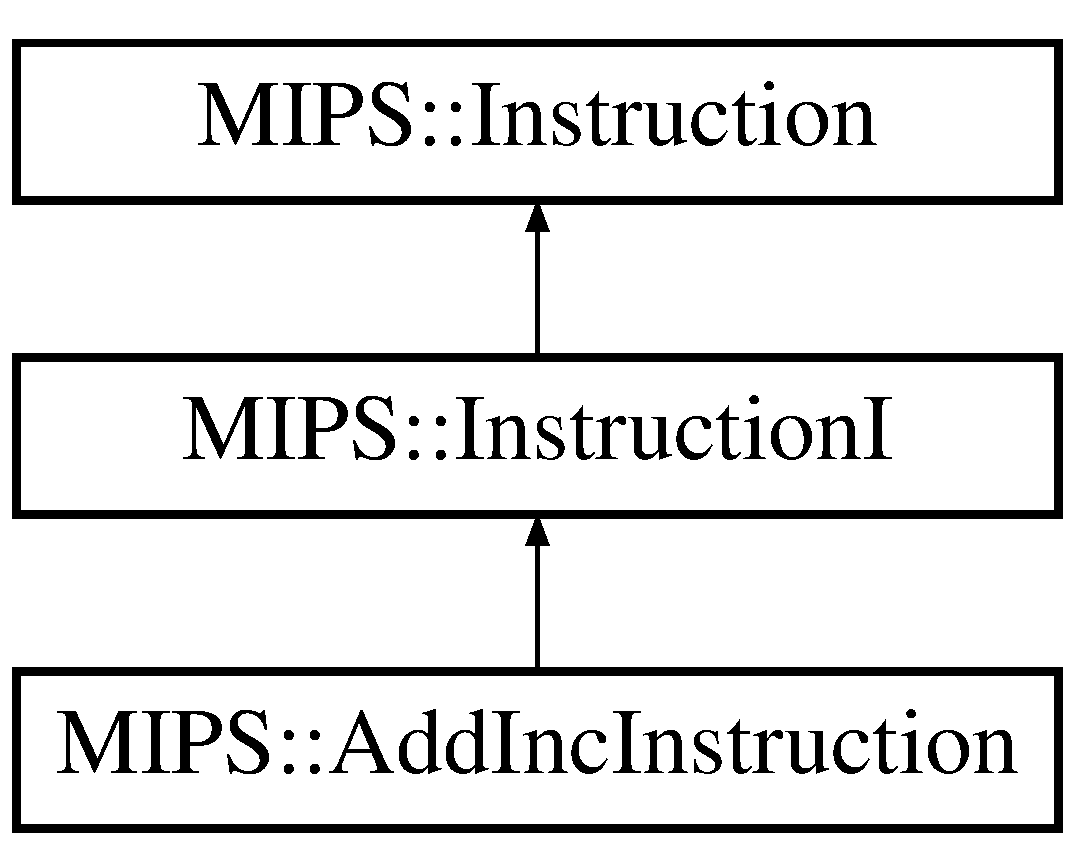
\includegraphics[height=3.000000cm]{classMIPS_1_1AddIncInstruction}
\end{center}
\end{figure}
\subsection*{Public Member Functions}
\begin{DoxyCompactItemize}
\item 
\hyperlink{classMIPS_1_1AddIncInstruction_a854d632650c4c1177d036fd8a1e85afb}{Add\+Inc\+Instruction} (\hyperlink{core_8hpp_a6074bae122ae7b527864eec42c728c3c}{bit8\+\_\+t} \hyperlink{classMIPS_1_1Instruction_a45cc6808b5dde8a5d41067d148b55476}{opcode}, \hyperlink{classMIPS_1_1Register}{Register} $\ast$\hyperlink{classMIPS_1_1InstructionI_a2be191d5b3dce505e2e626ec02eb4d62}{rs}, \hyperlink{classMIPS_1_1Register}{Register} $\ast$\hyperlink{classMIPS_1_1InstructionI_add1db07a5c954f35271de8c8a5737487}{rt}, \hyperlink{core_8hpp_a6074bae122ae7b527864eec42c728c3c}{bit8\+\_\+t} \hyperlink{classMIPS_1_1InstructionI_aa9b6da37c374c2ec8d96448d341e5e7d}{shamt}, \hyperlink{core_8hpp_a6074bae122ae7b527864eec42c728c3c}{bit8\+\_\+t} \hyperlink{classMIPS_1_1InstructionI_a5c6efcbbd233a7447c1fe24ea0a1e558}{funct})
\item 
\hyperlink{core_8hpp_adc265a970bc35995b5879784bbb3f1b7}{bit16\+\_\+t} \hyperlink{classMIPS_1_1AddIncInstruction_aa63fcaf17a9afc2f1b5d09a6291a70d6}{execute} ()
\end{DoxyCompactItemize}
\subsection*{Additional Inherited Members}


\subsection{Detailed Description}
Classe que faz a operação de A\+D\+D\+I\+NC no processador.

\begin{DoxyAuthor}{Author}
Felipe Dias 
\end{DoxyAuthor}


\subsection{Constructor \& Destructor Documentation}
\index{M\+I\+P\+S\+::\+Add\+Inc\+Instruction@{M\+I\+P\+S\+::\+Add\+Inc\+Instruction}!Add\+Inc\+Instruction@{Add\+Inc\+Instruction}}
\index{Add\+Inc\+Instruction@{Add\+Inc\+Instruction}!M\+I\+P\+S\+::\+Add\+Inc\+Instruction@{M\+I\+P\+S\+::\+Add\+Inc\+Instruction}}
\subsubsection[{\texorpdfstring{Add\+Inc\+Instruction(bit8\+\_\+t opcode, Register $\ast$rs, Register $\ast$rt, bit8\+\_\+t shamt, bit8\+\_\+t funct)}{AddIncInstruction(bit8_t opcode, Register *rs, Register *rt, bit8_t shamt, bit8_t funct)}}]{\setlength{\rightskip}{0pt plus 5cm}M\+I\+P\+S\+::\+Add\+Inc\+Instruction\+::\+Add\+Inc\+Instruction (
\begin{DoxyParamCaption}
\item[{{\bf bit8\+\_\+t}}]{opcode, }
\item[{{\bf Register} $\ast$}]{rs, }
\item[{{\bf Register} $\ast$}]{rt, }
\item[{{\bf bit8\+\_\+t}}]{shamt, }
\item[{{\bf bit8\+\_\+t}}]{funct}
\end{DoxyParamCaption}
)\hspace{0.3cm}{\ttfamily [inline]}}\hypertarget{classMIPS_1_1AddIncInstruction_a854d632650c4c1177d036fd8a1e85afb}{}\label{classMIPS_1_1AddIncInstruction_a854d632650c4c1177d036fd8a1e85afb}
Constroi uma nova instrução. 

\subsection{Member Function Documentation}
\index{M\+I\+P\+S\+::\+Add\+Inc\+Instruction@{M\+I\+P\+S\+::\+Add\+Inc\+Instruction}!execute@{execute}}
\index{execute@{execute}!M\+I\+P\+S\+::\+Add\+Inc\+Instruction@{M\+I\+P\+S\+::\+Add\+Inc\+Instruction}}
\subsubsection[{\texorpdfstring{execute()}{execute()}}]{\setlength{\rightskip}{0pt plus 5cm}{\bf bit16\+\_\+t} M\+I\+P\+S\+::\+Add\+Inc\+Instruction\+::execute (
\begin{DoxyParamCaption}
{}
\end{DoxyParamCaption}
)\hspace{0.3cm}{\ttfamily [virtual]}}\hypertarget{classMIPS_1_1AddIncInstruction_aa63fcaf17a9afc2f1b5d09a6291a70d6}{}\label{classMIPS_1_1AddIncInstruction_aa63fcaf17a9afc2f1b5d09a6291a70d6}
Função que executa a operação de soma.

\begin{DoxyReturn}{Returns}
resultado da operação 
\end{DoxyReturn}


Implements \hyperlink{classMIPS_1_1InstructionI_ae60fca5801bf5415cdff06d2aa11764f}{M\+I\+P\+S\+::\+InstructionI}.



The documentation for this class was generated from the following file\+:\begin{DoxyCompactItemize}
\item 
include/mips/instructions/format\+\_\+\+I/\hyperlink{addinc_8hpp}{addinc.\+hpp}\end{DoxyCompactItemize}

\hypertarget{classMIPS_1_1AddInstruction}{}\section{M\+I\+PS\+:\+:Add\+Instruction Class Reference}
\label{classMIPS_1_1AddInstruction}\index{M\+I\+P\+S\+::\+Add\+Instruction@{M\+I\+P\+S\+::\+Add\+Instruction}}


{\ttfamily \#include $<$add.\+hpp$>$}

Inheritance diagram for M\+I\+PS\+:\+:Add\+Instruction\+:\begin{figure}[H]
\begin{center}
\leavevmode
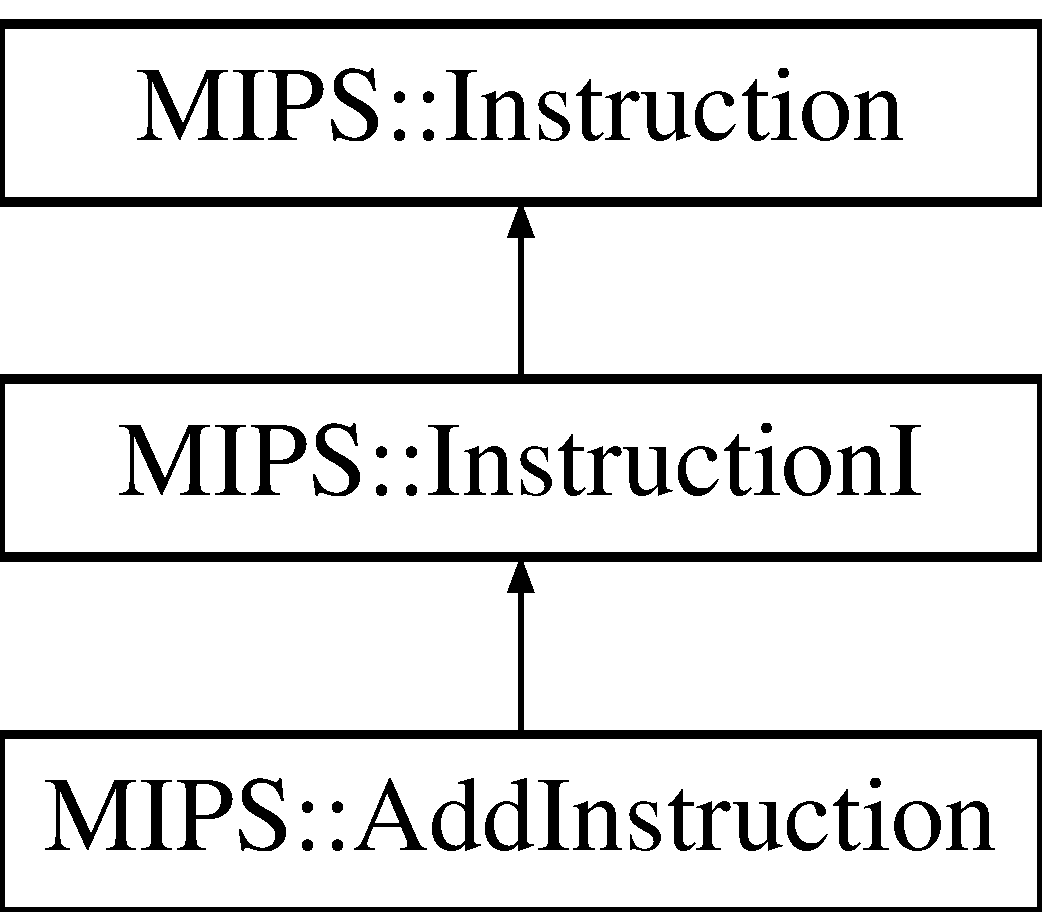
\includegraphics[height=3.000000cm]{classMIPS_1_1AddInstruction}
\end{center}
\end{figure}
\subsection*{Public Member Functions}
\begin{DoxyCompactItemize}
\item 
\hyperlink{classMIPS_1_1AddInstruction_a20874c9a6f6e0e5b5a1df2aa2d321c73}{Add\+Instruction} (\hyperlink{core_8hpp_a6074bae122ae7b527864eec42c728c3c}{bit8\+\_\+t} \hyperlink{classMIPS_1_1Instruction_a45cc6808b5dde8a5d41067d148b55476}{opcode}, \hyperlink{classMIPS_1_1Register}{Register} $\ast$\hyperlink{classMIPS_1_1InstructionI_a2be191d5b3dce505e2e626ec02eb4d62}{rs}, \hyperlink{classMIPS_1_1Register}{Register} $\ast$\hyperlink{classMIPS_1_1InstructionI_add1db07a5c954f35271de8c8a5737487}{rt}, \hyperlink{core_8hpp_a6074bae122ae7b527864eec42c728c3c}{bit8\+\_\+t} \hyperlink{classMIPS_1_1InstructionI_aa9b6da37c374c2ec8d96448d341e5e7d}{shamt}, \hyperlink{core_8hpp_a6074bae122ae7b527864eec42c728c3c}{bit8\+\_\+t} \hyperlink{classMIPS_1_1InstructionI_a5c6efcbbd233a7447c1fe24ea0a1e558}{funct})
\item 
\hyperlink{core_8hpp_adc265a970bc35995b5879784bbb3f1b7}{bit16\+\_\+t} \hyperlink{classMIPS_1_1AddInstruction_aa699dc00fdcd4250944f8afaa2fa89eb}{execute} ()
\end{DoxyCompactItemize}
\subsection*{Additional Inherited Members}


\subsection{Detailed Description}
Classe que faz a operação de A\+DD no processador.

\begin{DoxyAuthor}{Author}
Felipe Dias 
\end{DoxyAuthor}


\subsection{Constructor \& Destructor Documentation}
\index{M\+I\+P\+S\+::\+Add\+Instruction@{M\+I\+P\+S\+::\+Add\+Instruction}!Add\+Instruction@{Add\+Instruction}}
\index{Add\+Instruction@{Add\+Instruction}!M\+I\+P\+S\+::\+Add\+Instruction@{M\+I\+P\+S\+::\+Add\+Instruction}}
\subsubsection[{\texorpdfstring{Add\+Instruction(bit8\+\_\+t opcode, Register $\ast$rs, Register $\ast$rt, bit8\+\_\+t shamt, bit8\+\_\+t funct)}{AddInstruction(bit8_t opcode, Register *rs, Register *rt, bit8_t shamt, bit8_t funct)}}]{\setlength{\rightskip}{0pt plus 5cm}M\+I\+P\+S\+::\+Add\+Instruction\+::\+Add\+Instruction (
\begin{DoxyParamCaption}
\item[{{\bf bit8\+\_\+t}}]{opcode, }
\item[{{\bf Register} $\ast$}]{rs, }
\item[{{\bf Register} $\ast$}]{rt, }
\item[{{\bf bit8\+\_\+t}}]{shamt, }
\item[{{\bf bit8\+\_\+t}}]{funct}
\end{DoxyParamCaption}
)\hspace{0.3cm}{\ttfamily [inline]}}\hypertarget{classMIPS_1_1AddInstruction_a20874c9a6f6e0e5b5a1df2aa2d321c73}{}\label{classMIPS_1_1AddInstruction_a20874c9a6f6e0e5b5a1df2aa2d321c73}
Constroi uma nova instrução. 

\subsection{Member Function Documentation}
\index{M\+I\+P\+S\+::\+Add\+Instruction@{M\+I\+P\+S\+::\+Add\+Instruction}!execute@{execute}}
\index{execute@{execute}!M\+I\+P\+S\+::\+Add\+Instruction@{M\+I\+P\+S\+::\+Add\+Instruction}}
\subsubsection[{\texorpdfstring{execute()}{execute()}}]{\setlength{\rightskip}{0pt plus 5cm}{\bf bit16\+\_\+t} M\+I\+P\+S\+::\+Add\+Instruction\+::execute (
\begin{DoxyParamCaption}
{}
\end{DoxyParamCaption}
)\hspace{0.3cm}{\ttfamily [virtual]}}\hypertarget{classMIPS_1_1AddInstruction_aa699dc00fdcd4250944f8afaa2fa89eb}{}\label{classMIPS_1_1AddInstruction_aa699dc00fdcd4250944f8afaa2fa89eb}
Função que executa a operação de soma.

\begin{DoxyReturn}{Returns}
resultado da operação 
\end{DoxyReturn}


Implements \hyperlink{classMIPS_1_1InstructionI_ae60fca5801bf5415cdff06d2aa11764f}{M\+I\+P\+S\+::\+InstructionI}.



The documentation for this class was generated from the following file\+:\begin{DoxyCompactItemize}
\item 
include/mips/instructions/format\+\_\+\+I/\hyperlink{add_8hpp}{add.\+hpp}\end{DoxyCompactItemize}

\hypertarget{structMIPS_1_1ALUFlags}{}\section{M\+I\+PS\+:\+:A\+L\+U\+Flags Struct Reference}
\label{structMIPS_1_1ALUFlags}\index{M\+I\+P\+S\+::\+A\+L\+U\+Flags@{M\+I\+P\+S\+::\+A\+L\+U\+Flags}}


{\ttfamily \#include $<$flag.\+hpp$>$}

\subsection*{Public Attributes}
\begin{DoxyCompactItemize}
\item 
\hyperlink{core_8hpp_a6074bae122ae7b527864eec42c728c3c}{bit8\+\_\+t} \hyperlink{structMIPS_1_1ALUFlags_a75e610fd16cb450f1870c9fb672125eb}{zero}\hypertarget{structMIPS_1_1ALUFlags_a75e610fd16cb450f1870c9fb672125eb}{}\label{structMIPS_1_1ALUFlags_a75e610fd16cb450f1870c9fb672125eb}

\begin{DoxyCompactList}\small\item\em Flag de zero. \end{DoxyCompactList}\item 
\hyperlink{core_8hpp_a6074bae122ae7b527864eec42c728c3c}{bit8\+\_\+t} \hyperlink{structMIPS_1_1ALUFlags_aa00c4b1911180ec6ce00126f3475a5ba}{carry}\hypertarget{structMIPS_1_1ALUFlags_aa00c4b1911180ec6ce00126f3475a5ba}{}\label{structMIPS_1_1ALUFlags_aa00c4b1911180ec6ce00126f3475a5ba}

\begin{DoxyCompactList}\small\item\em Flag de carry. \end{DoxyCompactList}\item 
\hyperlink{core_8hpp_a6074bae122ae7b527864eec42c728c3c}{bit8\+\_\+t} \hyperlink{structMIPS_1_1ALUFlags_a9183433b8cc39c500f8039d34d329b3d}{neg}\hypertarget{structMIPS_1_1ALUFlags_a9183433b8cc39c500f8039d34d329b3d}{}\label{structMIPS_1_1ALUFlags_a9183433b8cc39c500f8039d34d329b3d}

\begin{DoxyCompactList}\small\item\em Flag de negativo. \end{DoxyCompactList}\item 
\hyperlink{core_8hpp_a6074bae122ae7b527864eec42c728c3c}{bit8\+\_\+t} \hyperlink{structMIPS_1_1ALUFlags_a9f3ea56726a1e5f09fd13d8f7be3c234}{overflow}\hypertarget{structMIPS_1_1ALUFlags_a9f3ea56726a1e5f09fd13d8f7be3c234}{}\label{structMIPS_1_1ALUFlags_a9f3ea56726a1e5f09fd13d8f7be3c234}

\begin{DoxyCompactList}\small\item\em Flag de overflow. \end{DoxyCompactList}\end{DoxyCompactItemize}


\subsection{Detailed Description}
Estrutura que armazena as informações das flags de saída da A\+LU. 

The documentation for this struct was generated from the following file\+:\begin{DoxyCompactItemize}
\item 
include/mips/\hyperlink{flag_8hpp}{flag.\+hpp}\end{DoxyCompactItemize}

\hypertarget{classMIPS_1_1AndInstruction}{}\section{M\+I\+PS\+:\+:And\+Instruction Class Reference}
\label{classMIPS_1_1AndInstruction}\index{M\+I\+P\+S\+::\+And\+Instruction@{M\+I\+P\+S\+::\+And\+Instruction}}


{\ttfamily \#include $<$and.\+hpp$>$}

Inheritance diagram for M\+I\+PS\+:\+:And\+Instruction\+:\begin{figure}[H]
\begin{center}
\leavevmode
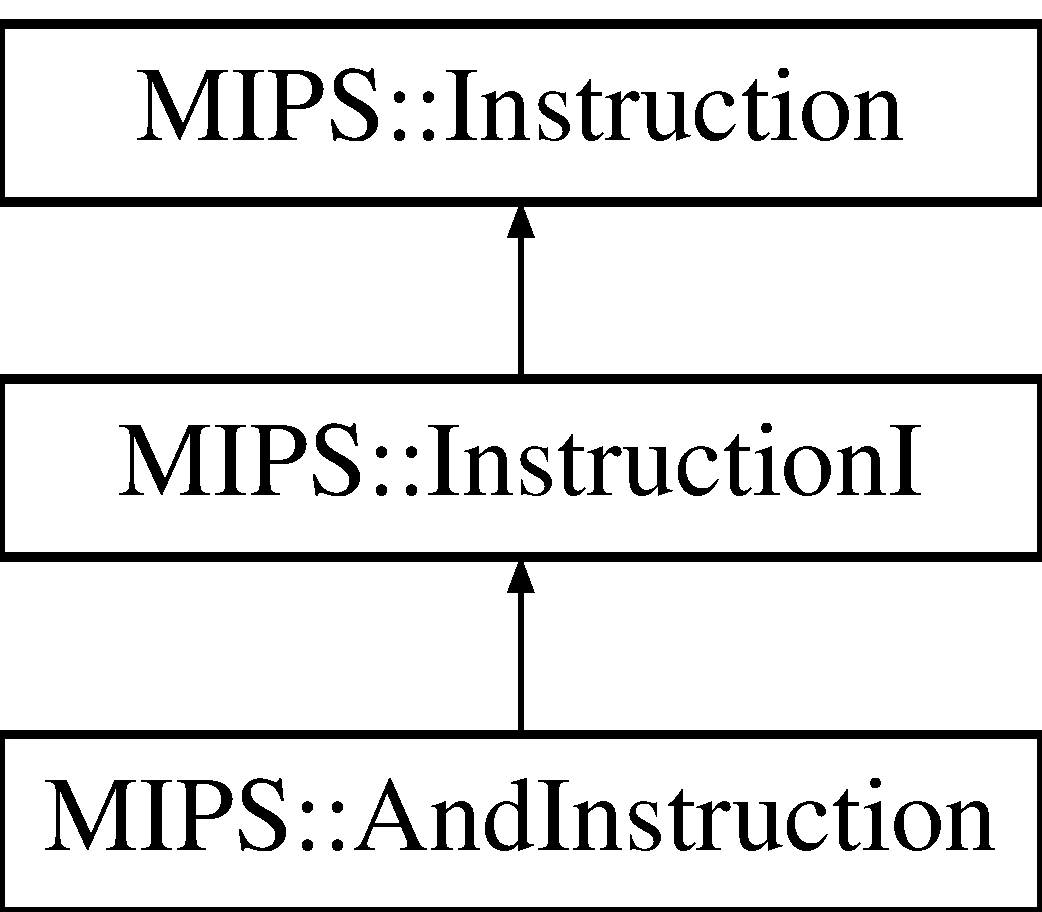
\includegraphics[height=3.000000cm]{classMIPS_1_1AndInstruction}
\end{center}
\end{figure}
\subsection*{Public Member Functions}
\begin{DoxyCompactItemize}
\item 
\hyperlink{classMIPS_1_1AndInstruction_a9cc655d129040fe504607d0a3a06f942}{And\+Instruction} (\hyperlink{core_8hpp_a6074bae122ae7b527864eec42c728c3c}{bit8\+\_\+t} \hyperlink{classMIPS_1_1Instruction_a45cc6808b5dde8a5d41067d148b55476}{opcode}, \hyperlink{classMIPS_1_1Register}{Register} $\ast$\hyperlink{classMIPS_1_1InstructionI_a2be191d5b3dce505e2e626ec02eb4d62}{rs}, \hyperlink{classMIPS_1_1Register}{Register} $\ast$\hyperlink{classMIPS_1_1InstructionI_add1db07a5c954f35271de8c8a5737487}{rt}, \hyperlink{core_8hpp_a6074bae122ae7b527864eec42c728c3c}{bit8\+\_\+t} \hyperlink{classMIPS_1_1InstructionI_aa9b6da37c374c2ec8d96448d341e5e7d}{shamt}, \hyperlink{core_8hpp_a6074bae122ae7b527864eec42c728c3c}{bit8\+\_\+t} \hyperlink{classMIPS_1_1InstructionI_a5c6efcbbd233a7447c1fe24ea0a1e558}{funct})
\item 
\hyperlink{core_8hpp_adc265a970bc35995b5879784bbb3f1b7}{bit16\+\_\+t} \hyperlink{classMIPS_1_1AndInstruction_a24b2fdb68ff022275db4181e502b7a48}{execute} ()
\end{DoxyCompactItemize}
\subsection*{Additional Inherited Members}


\subsection{Detailed Description}
Classe que faz a operação de and no processador.

\begin{DoxyAuthor}{Author}
Lucas Fonseca dos Santos 
\end{DoxyAuthor}


\subsection{Constructor \& Destructor Documentation}
\index{M\+I\+P\+S\+::\+And\+Instruction@{M\+I\+P\+S\+::\+And\+Instruction}!And\+Instruction@{And\+Instruction}}
\index{And\+Instruction@{And\+Instruction}!M\+I\+P\+S\+::\+And\+Instruction@{M\+I\+P\+S\+::\+And\+Instruction}}
\subsubsection[{\texorpdfstring{And\+Instruction(bit8\+\_\+t opcode, Register $\ast$rs, Register $\ast$rt, bit8\+\_\+t shamt, bit8\+\_\+t funct)}{AndInstruction(bit8_t opcode, Register *rs, Register *rt, bit8_t shamt, bit8_t funct)}}]{\setlength{\rightskip}{0pt plus 5cm}M\+I\+P\+S\+::\+And\+Instruction\+::\+And\+Instruction (
\begin{DoxyParamCaption}
\item[{{\bf bit8\+\_\+t}}]{opcode, }
\item[{{\bf Register} $\ast$}]{rs, }
\item[{{\bf Register} $\ast$}]{rt, }
\item[{{\bf bit8\+\_\+t}}]{shamt, }
\item[{{\bf bit8\+\_\+t}}]{funct}
\end{DoxyParamCaption}
)\hspace{0.3cm}{\ttfamily [inline]}}\hypertarget{classMIPS_1_1AndInstruction_a9cc655d129040fe504607d0a3a06f942}{}\label{classMIPS_1_1AndInstruction_a9cc655d129040fe504607d0a3a06f942}
Constroi uma nova instrução. 

\subsection{Member Function Documentation}
\index{M\+I\+P\+S\+::\+And\+Instruction@{M\+I\+P\+S\+::\+And\+Instruction}!execute@{execute}}
\index{execute@{execute}!M\+I\+P\+S\+::\+And\+Instruction@{M\+I\+P\+S\+::\+And\+Instruction}}
\subsubsection[{\texorpdfstring{execute()}{execute()}}]{\setlength{\rightskip}{0pt plus 5cm}{\bf bit16\+\_\+t} M\+I\+P\+S\+::\+And\+Instruction\+::execute (
\begin{DoxyParamCaption}
{}
\end{DoxyParamCaption}
)\hspace{0.3cm}{\ttfamily [virtual]}}\hypertarget{classMIPS_1_1AndInstruction_a24b2fdb68ff022275db4181e502b7a48}{}\label{classMIPS_1_1AndInstruction_a24b2fdb68ff022275db4181e502b7a48}
Função que executa a operação de \hyperlink{classMIPS_1_1AndInstruction}{And\+Instruction}. 

Implements \hyperlink{classMIPS_1_1InstructionI_ae60fca5801bf5415cdff06d2aa11764f}{M\+I\+P\+S\+::\+InstructionI}.



The documentation for this class was generated from the following file\+:\begin{DoxyCompactItemize}
\item 
include/mips/instructions/format\+\_\+\+I/\hyperlink{and_8hpp}{and.\+hpp}\end{DoxyCompactItemize}

\hypertarget{classMIPS_1_1AndnotaInstruction}{}\section{M\+I\+PS\+:\+:Andnota\+Instruction Class Reference}
\label{classMIPS_1_1AndnotaInstruction}\index{M\+I\+P\+S\+::\+Andnota\+Instruction@{M\+I\+P\+S\+::\+Andnota\+Instruction}}


{\ttfamily \#include $<$andnota.\+hpp$>$}

Inheritance diagram for M\+I\+PS\+:\+:Andnota\+Instruction\+:\begin{figure}[H]
\begin{center}
\leavevmode
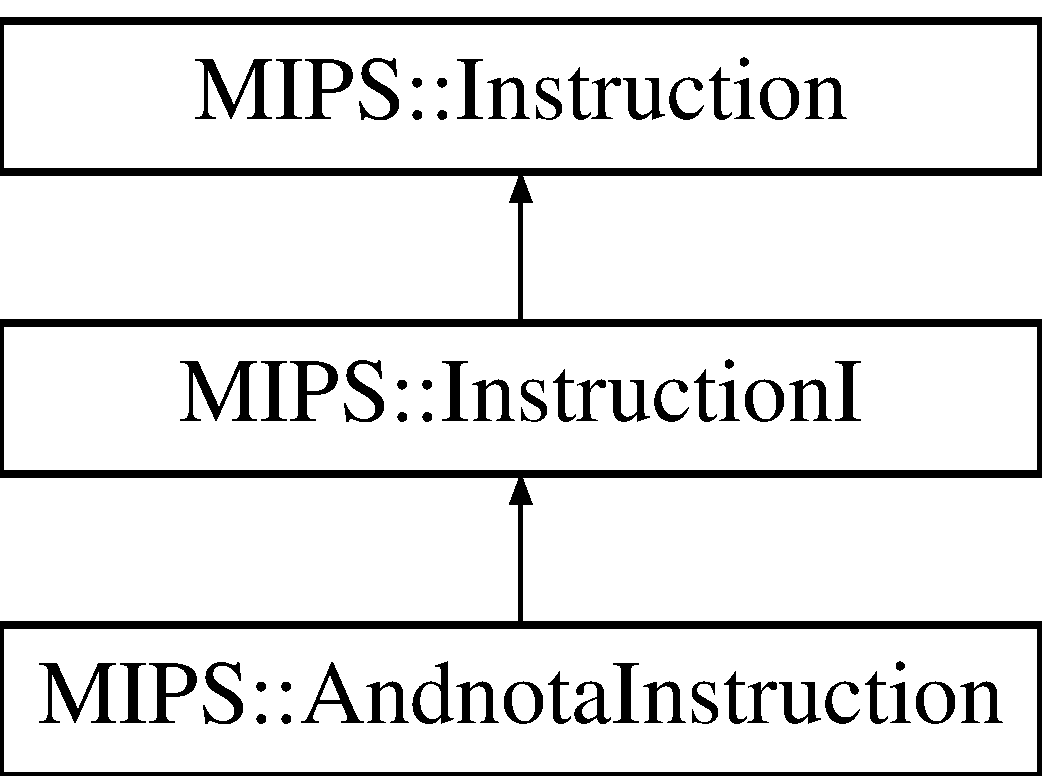
\includegraphics[height=3.000000cm]{classMIPS_1_1AndnotaInstruction}
\end{center}
\end{figure}
\subsection*{Public Member Functions}
\begin{DoxyCompactItemize}
\item 
\hyperlink{classMIPS_1_1AndnotaInstruction_aaa02f585a018e3194fc4b3fc0b2f4b04}{Andnota\+Instruction} (\hyperlink{core_8hpp_a6074bae122ae7b527864eec42c728c3c}{bit8\+\_\+t} \hyperlink{classMIPS_1_1Instruction_a45cc6808b5dde8a5d41067d148b55476}{opcode}, \hyperlink{classMIPS_1_1Register}{Register} $\ast$\hyperlink{classMIPS_1_1InstructionI_a2be191d5b3dce505e2e626ec02eb4d62}{rs}, \hyperlink{classMIPS_1_1Register}{Register} $\ast$\hyperlink{classMIPS_1_1InstructionI_add1db07a5c954f35271de8c8a5737487}{rt}, \hyperlink{core_8hpp_a6074bae122ae7b527864eec42c728c3c}{bit8\+\_\+t} \hyperlink{classMIPS_1_1InstructionI_aa9b6da37c374c2ec8d96448d341e5e7d}{shamt}, \hyperlink{core_8hpp_a6074bae122ae7b527864eec42c728c3c}{bit8\+\_\+t} \hyperlink{classMIPS_1_1InstructionI_a5c6efcbbd233a7447c1fe24ea0a1e558}{funct})
\item 
\hyperlink{core_8hpp_adc265a970bc35995b5879784bbb3f1b7}{bit16\+\_\+t} \hyperlink{classMIPS_1_1AndnotaInstruction_afdc3b2836318f4adaa32dfa3bcdf7c45}{execute} ()
\end{DoxyCompactItemize}
\subsection*{Additional Inherited Members}


\subsection{Detailed Description}
Classe que faz a operação de andnota no processador.

\begin{DoxyAuthor}{Author}
Lucas Pereira 
\end{DoxyAuthor}


\subsection{Constructor \& Destructor Documentation}
\index{M\+I\+P\+S\+::\+Andnota\+Instruction@{M\+I\+P\+S\+::\+Andnota\+Instruction}!Andnota\+Instruction@{Andnota\+Instruction}}
\index{Andnota\+Instruction@{Andnota\+Instruction}!M\+I\+P\+S\+::\+Andnota\+Instruction@{M\+I\+P\+S\+::\+Andnota\+Instruction}}
\subsubsection[{\texorpdfstring{Andnota\+Instruction(bit8\+\_\+t opcode, Register $\ast$rs, Register $\ast$rt, bit8\+\_\+t shamt, bit8\+\_\+t funct)}{AndnotaInstruction(bit8_t opcode, Register *rs, Register *rt, bit8_t shamt, bit8_t funct)}}]{\setlength{\rightskip}{0pt plus 5cm}M\+I\+P\+S\+::\+Andnota\+Instruction\+::\+Andnota\+Instruction (
\begin{DoxyParamCaption}
\item[{{\bf bit8\+\_\+t}}]{opcode, }
\item[{{\bf Register} $\ast$}]{rs, }
\item[{{\bf Register} $\ast$}]{rt, }
\item[{{\bf bit8\+\_\+t}}]{shamt, }
\item[{{\bf bit8\+\_\+t}}]{funct}
\end{DoxyParamCaption}
)\hspace{0.3cm}{\ttfamily [inline]}}\hypertarget{classMIPS_1_1AndnotaInstruction_aaa02f585a018e3194fc4b3fc0b2f4b04}{}\label{classMIPS_1_1AndnotaInstruction_aaa02f585a018e3194fc4b3fc0b2f4b04}
Constroi uma nova instrução. 

\subsection{Member Function Documentation}
\index{M\+I\+P\+S\+::\+Andnota\+Instruction@{M\+I\+P\+S\+::\+Andnota\+Instruction}!execute@{execute}}
\index{execute@{execute}!M\+I\+P\+S\+::\+Andnota\+Instruction@{M\+I\+P\+S\+::\+Andnota\+Instruction}}
\subsubsection[{\texorpdfstring{execute()}{execute()}}]{\setlength{\rightskip}{0pt plus 5cm}{\bf bit16\+\_\+t} M\+I\+P\+S\+::\+Andnota\+Instruction\+::execute (
\begin{DoxyParamCaption}
{}
\end{DoxyParamCaption}
)\hspace{0.3cm}{\ttfamily [virtual]}}\hypertarget{classMIPS_1_1AndnotaInstruction_afdc3b2836318f4adaa32dfa3bcdf7c45}{}\label{classMIPS_1_1AndnotaInstruction_afdc3b2836318f4adaa32dfa3bcdf7c45}
Função que executa a operação de \hyperlink{classMIPS_1_1AndnotaInstruction}{Andnota\+Instruction}.

\begin{DoxyReturn}{Returns}
resultado da operação 
\end{DoxyReturn}


Implements \hyperlink{classMIPS_1_1InstructionI_ae60fca5801bf5415cdff06d2aa11764f}{M\+I\+P\+S\+::\+InstructionI}.



The documentation for this class was generated from the following file\+:\begin{DoxyCompactItemize}
\item 
include/mips/instructions/format\+\_\+\+I/\hyperlink{andnota_8hpp}{andnota.\+hpp}\end{DoxyCompactItemize}

\hypertarget{classMIPS_1_1AslInstruction}{}\section{M\+I\+PS\+:\+:Asl\+Instruction Class Reference}
\label{classMIPS_1_1AslInstruction}\index{M\+I\+P\+S\+::\+Asl\+Instruction@{M\+I\+P\+S\+::\+Asl\+Instruction}}


{\ttfamily \#include $<$asl.\+hpp$>$}

Inheritance diagram for M\+I\+PS\+:\+:Asl\+Instruction\+:\begin{figure}[H]
\begin{center}
\leavevmode
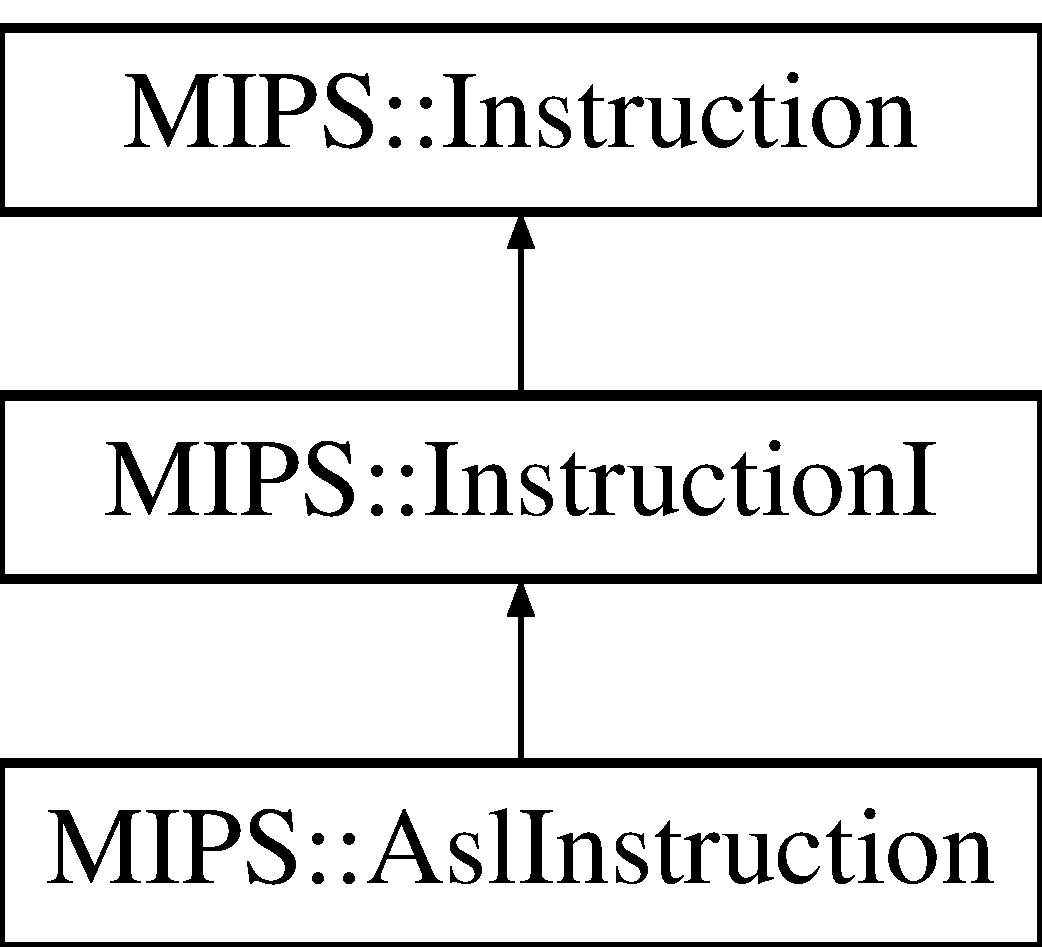
\includegraphics[height=3.000000cm]{classMIPS_1_1AslInstruction}
\end{center}
\end{figure}
\subsection*{Public Member Functions}
\begin{DoxyCompactItemize}
\item 
\hyperlink{classMIPS_1_1AslInstruction_ada0aa9e794e21cf178e349a38ec4716f}{Asl\+Instruction} (\hyperlink{core_8hpp_a6074bae122ae7b527864eec42c728c3c}{bit8\+\_\+t} \hyperlink{classMIPS_1_1Instruction_a45cc6808b5dde8a5d41067d148b55476}{opcode}, \hyperlink{classMIPS_1_1Register}{Register} $\ast$\hyperlink{classMIPS_1_1InstructionI_a2be191d5b3dce505e2e626ec02eb4d62}{rs}, \hyperlink{classMIPS_1_1Register}{Register} $\ast$\hyperlink{classMIPS_1_1InstructionI_add1db07a5c954f35271de8c8a5737487}{rt}, \hyperlink{core_8hpp_a6074bae122ae7b527864eec42c728c3c}{bit8\+\_\+t} \hyperlink{classMIPS_1_1InstructionI_aa9b6da37c374c2ec8d96448d341e5e7d}{shamt}, \hyperlink{core_8hpp_a6074bae122ae7b527864eec42c728c3c}{bit8\+\_\+t} \hyperlink{classMIPS_1_1InstructionI_a5c6efcbbd233a7447c1fe24ea0a1e558}{funct})
\item 
\hyperlink{core_8hpp_adc265a970bc35995b5879784bbb3f1b7}{bit16\+\_\+t} \hyperlink{classMIPS_1_1AslInstruction_adafc2d1f549cda9bdf757dc2bac03ca9}{execute} ()
\end{DoxyCompactItemize}
\subsection*{Additional Inherited Members}


\subsection{Detailed Description}
Classe que faz a operação de A\+SR no processador.

\begin{DoxyAuthor}{Author}
Felipe Dias 
\end{DoxyAuthor}


\subsection{Constructor \& Destructor Documentation}
\index{M\+I\+P\+S\+::\+Asl\+Instruction@{M\+I\+P\+S\+::\+Asl\+Instruction}!Asl\+Instruction@{Asl\+Instruction}}
\index{Asl\+Instruction@{Asl\+Instruction}!M\+I\+P\+S\+::\+Asl\+Instruction@{M\+I\+P\+S\+::\+Asl\+Instruction}}
\subsubsection[{\texorpdfstring{Asl\+Instruction(bit8\+\_\+t opcode, Register $\ast$rs, Register $\ast$rt, bit8\+\_\+t shamt, bit8\+\_\+t funct)}{AslInstruction(bit8_t opcode, Register *rs, Register *rt, bit8_t shamt, bit8_t funct)}}]{\setlength{\rightskip}{0pt plus 5cm}M\+I\+P\+S\+::\+Asl\+Instruction\+::\+Asl\+Instruction (
\begin{DoxyParamCaption}
\item[{{\bf bit8\+\_\+t}}]{opcode, }
\item[{{\bf Register} $\ast$}]{rs, }
\item[{{\bf Register} $\ast$}]{rt, }
\item[{{\bf bit8\+\_\+t}}]{shamt, }
\item[{{\bf bit8\+\_\+t}}]{funct}
\end{DoxyParamCaption}
)\hspace{0.3cm}{\ttfamily [inline]}}\hypertarget{classMIPS_1_1AslInstruction_ada0aa9e794e21cf178e349a38ec4716f}{}\label{classMIPS_1_1AslInstruction_ada0aa9e794e21cf178e349a38ec4716f}
Constroi uma nova instrução. 

\subsection{Member Function Documentation}
\index{M\+I\+P\+S\+::\+Asl\+Instruction@{M\+I\+P\+S\+::\+Asl\+Instruction}!execute@{execute}}
\index{execute@{execute}!M\+I\+P\+S\+::\+Asl\+Instruction@{M\+I\+P\+S\+::\+Asl\+Instruction}}
\subsubsection[{\texorpdfstring{execute()}{execute()}}]{\setlength{\rightskip}{0pt plus 5cm}{\bf bit16\+\_\+t} M\+I\+P\+S\+::\+Asl\+Instruction\+::execute (
\begin{DoxyParamCaption}
{}
\end{DoxyParamCaption}
)\hspace{0.3cm}{\ttfamily [virtual]}}\hypertarget{classMIPS_1_1AslInstruction_adafc2d1f549cda9bdf757dc2bac03ca9}{}\label{classMIPS_1_1AslInstruction_adafc2d1f549cda9bdf757dc2bac03ca9}
Função que executa a operação de shift a esquerda.

\begin{DoxyReturn}{Returns}
resultado da operação 
\end{DoxyReturn}


Implements \hyperlink{classMIPS_1_1InstructionI_ae60fca5801bf5415cdff06d2aa11764f}{M\+I\+P\+S\+::\+InstructionI}.



The documentation for this class was generated from the following file\+:\begin{DoxyCompactItemize}
\item 
include/mips/instructions/format\+\_\+\+I/asl.\+hpp\end{DoxyCompactItemize}

\hypertarget{classMIPS_1_1AsrInstruction}{}\section{M\+I\+PS\+:\+:Asr\+Instruction Class Reference}
\label{classMIPS_1_1AsrInstruction}\index{M\+I\+P\+S\+::\+Asr\+Instruction@{M\+I\+P\+S\+::\+Asr\+Instruction}}


{\ttfamily \#include $<$asr.\+hpp$>$}

Inheritance diagram for M\+I\+PS\+:\+:Asr\+Instruction\+:\begin{figure}[H]
\begin{center}
\leavevmode
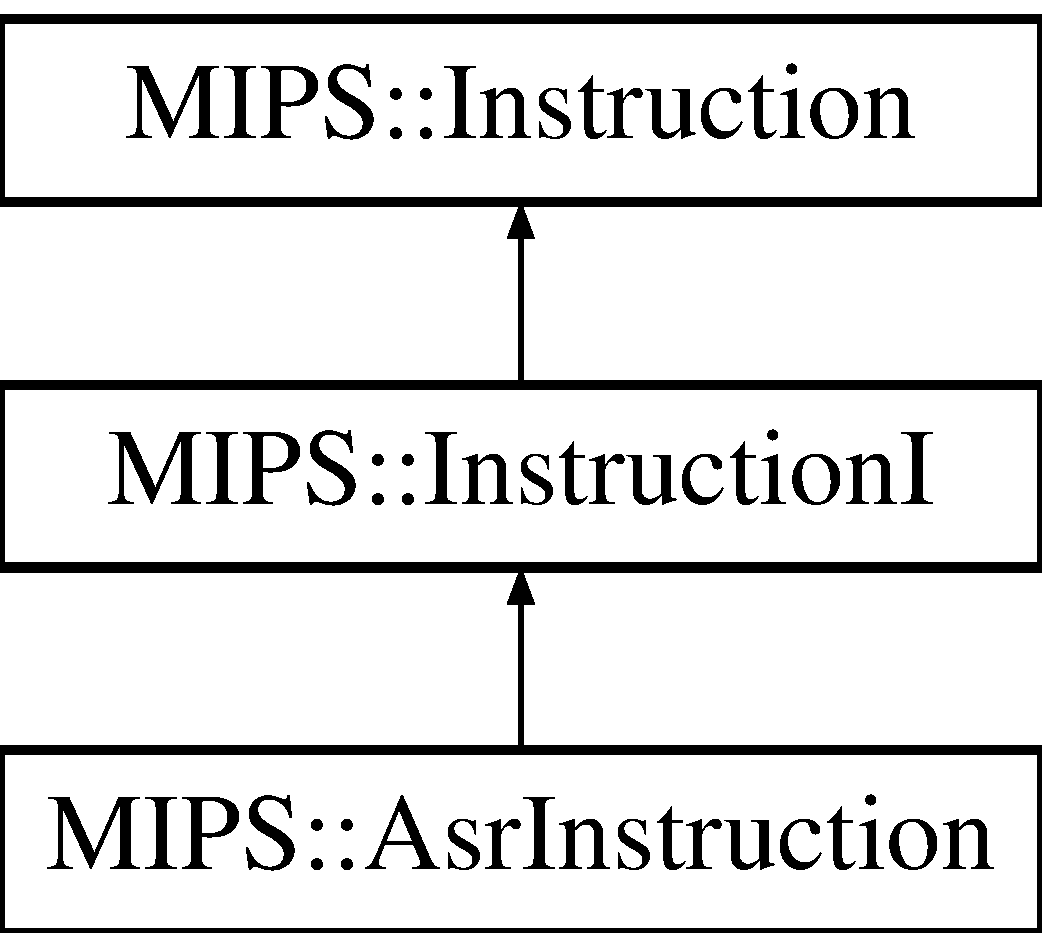
\includegraphics[height=3.000000cm]{classMIPS_1_1AsrInstruction}
\end{center}
\end{figure}
\subsection*{Public Member Functions}
\begin{DoxyCompactItemize}
\item 
\hyperlink{classMIPS_1_1AsrInstruction_ae354d9deabc5e23bf244cb8907bb83cb}{Asr\+Instruction} (\hyperlink{core_8hpp_a6074bae122ae7b527864eec42c728c3c}{bit8\+\_\+t} \hyperlink{classMIPS_1_1Instruction_a45cc6808b5dde8a5d41067d148b55476}{opcode}, \hyperlink{classMIPS_1_1Register}{Register} $\ast$\hyperlink{classMIPS_1_1InstructionI_a2be191d5b3dce505e2e626ec02eb4d62}{rs}, \hyperlink{classMIPS_1_1Register}{Register} $\ast$\hyperlink{classMIPS_1_1InstructionI_add1db07a5c954f35271de8c8a5737487}{rt}, \hyperlink{core_8hpp_a6074bae122ae7b527864eec42c728c3c}{bit8\+\_\+t} \hyperlink{classMIPS_1_1InstructionI_aa9b6da37c374c2ec8d96448d341e5e7d}{shamt}, \hyperlink{core_8hpp_a6074bae122ae7b527864eec42c728c3c}{bit8\+\_\+t} \hyperlink{classMIPS_1_1InstructionI_a5c6efcbbd233a7447c1fe24ea0a1e558}{funct})
\item 
\hyperlink{core_8hpp_adc265a970bc35995b5879784bbb3f1b7}{bit16\+\_\+t} \hyperlink{classMIPS_1_1AsrInstruction_aad46283e10517abf6bf5e527ca020d53}{execute} ()
\end{DoxyCompactItemize}
\subsection*{Additional Inherited Members}


\subsection{Detailed Description}
Classe que faz a operação de A\+SR no processador.

\begin{DoxyAuthor}{Author}
Felipe Dias 
\end{DoxyAuthor}


\subsection{Constructor \& Destructor Documentation}
\index{M\+I\+P\+S\+::\+Asr\+Instruction@{M\+I\+P\+S\+::\+Asr\+Instruction}!Asr\+Instruction@{Asr\+Instruction}}
\index{Asr\+Instruction@{Asr\+Instruction}!M\+I\+P\+S\+::\+Asr\+Instruction@{M\+I\+P\+S\+::\+Asr\+Instruction}}
\subsubsection[{\texorpdfstring{Asr\+Instruction(bit8\+\_\+t opcode, Register $\ast$rs, Register $\ast$rt, bit8\+\_\+t shamt, bit8\+\_\+t funct)}{AsrInstruction(bit8_t opcode, Register *rs, Register *rt, bit8_t shamt, bit8_t funct)}}]{\setlength{\rightskip}{0pt plus 5cm}M\+I\+P\+S\+::\+Asr\+Instruction\+::\+Asr\+Instruction (
\begin{DoxyParamCaption}
\item[{{\bf bit8\+\_\+t}}]{opcode, }
\item[{{\bf Register} $\ast$}]{rs, }
\item[{{\bf Register} $\ast$}]{rt, }
\item[{{\bf bit8\+\_\+t}}]{shamt, }
\item[{{\bf bit8\+\_\+t}}]{funct}
\end{DoxyParamCaption}
)\hspace{0.3cm}{\ttfamily [inline]}}\hypertarget{classMIPS_1_1AsrInstruction_ae354d9deabc5e23bf244cb8907bb83cb}{}\label{classMIPS_1_1AsrInstruction_ae354d9deabc5e23bf244cb8907bb83cb}
Constroi uma nova instrução. 

\subsection{Member Function Documentation}
\index{M\+I\+P\+S\+::\+Asr\+Instruction@{M\+I\+P\+S\+::\+Asr\+Instruction}!execute@{execute}}
\index{execute@{execute}!M\+I\+P\+S\+::\+Asr\+Instruction@{M\+I\+P\+S\+::\+Asr\+Instruction}}
\subsubsection[{\texorpdfstring{execute()}{execute()}}]{\setlength{\rightskip}{0pt plus 5cm}{\bf bit16\+\_\+t} M\+I\+P\+S\+::\+Asr\+Instruction\+::execute (
\begin{DoxyParamCaption}
{}
\end{DoxyParamCaption}
)\hspace{0.3cm}{\ttfamily [virtual]}}\hypertarget{classMIPS_1_1AsrInstruction_aad46283e10517abf6bf5e527ca020d53}{}\label{classMIPS_1_1AsrInstruction_aad46283e10517abf6bf5e527ca020d53}
Função que executa a operação de shift a direita.

\begin{DoxyReturn}{Returns}
resultado da operação 
\end{DoxyReturn}


Implements \hyperlink{classMIPS_1_1InstructionI_ae60fca5801bf5415cdff06d2aa11764f}{M\+I\+P\+S\+::\+InstructionI}.



The documentation for this class was generated from the following file\+:\begin{DoxyCompactItemize}
\item 
include/mips/instructions/format\+\_\+\+I/asr.\+hpp\end{DoxyCompactItemize}

\hypertarget{classMIPS_1_1ControlUnit}{}\section{M\+I\+PS\+:\+:Control\+Unit Class Reference}
\label{classMIPS_1_1ControlUnit}\index{M\+I\+P\+S\+::\+Control\+Unit@{M\+I\+P\+S\+::\+Control\+Unit}}


{\ttfamily \#include $<$control.\+hpp$>$}

\subsection*{Public Member Functions}
\begin{DoxyCompactItemize}
\item 
\hyperlink{classMIPS_1_1ControlUnit_a4e7f136cf15bc78b878082ba5fe5b629}{Control\+Unit} ()
\item 
\hyperlink{classMIPS_1_1ControlUnit_a6e1a1d7cd85594c9a575a432770c3aa2}{$\sim$\+Control\+Unit} ()
\end{DoxyCompactItemize}


\subsection{Detailed Description}
Unidade de controle do processador. Essa unidade é responsável por setar todas as flags que serão utilizadas para executar uma instrução.

\begin{DoxyAuthor}{Author}
Matheus Nogueira 
\end{DoxyAuthor}


\subsection{Constructor \& Destructor Documentation}
\index{M\+I\+P\+S\+::\+Control\+Unit@{M\+I\+P\+S\+::\+Control\+Unit}!Control\+Unit@{Control\+Unit}}
\index{Control\+Unit@{Control\+Unit}!M\+I\+P\+S\+::\+Control\+Unit@{M\+I\+P\+S\+::\+Control\+Unit}}
\subsubsection[{\texorpdfstring{Control\+Unit()}{ControlUnit()}}]{\setlength{\rightskip}{0pt plus 5cm}M\+I\+P\+S\+::\+Control\+Unit\+::\+Control\+Unit (
\begin{DoxyParamCaption}
{}
\end{DoxyParamCaption}
)}\hypertarget{classMIPS_1_1ControlUnit_a4e7f136cf15bc78b878082ba5fe5b629}{}\label{classMIPS_1_1ControlUnit_a4e7f136cf15bc78b878082ba5fe5b629}
Cria uma nova unidade de controle. \index{M\+I\+P\+S\+::\+Control\+Unit@{M\+I\+P\+S\+::\+Control\+Unit}!````~Control\+Unit@{$\sim$\+Control\+Unit}}
\index{````~Control\+Unit@{$\sim$\+Control\+Unit}!M\+I\+P\+S\+::\+Control\+Unit@{M\+I\+P\+S\+::\+Control\+Unit}}
\subsubsection[{\texorpdfstring{$\sim$\+Control\+Unit()}{~ControlUnit()}}]{\setlength{\rightskip}{0pt plus 5cm}M\+I\+P\+S\+::\+Control\+Unit\+::$\sim$\+Control\+Unit (
\begin{DoxyParamCaption}
{}
\end{DoxyParamCaption}
)}\hypertarget{classMIPS_1_1ControlUnit_a6e1a1d7cd85594c9a575a432770c3aa2}{}\label{classMIPS_1_1ControlUnit_a6e1a1d7cd85594c9a575a432770c3aa2}
Destroi a unidade de controle. 

The documentation for this class was generated from the following file\+:\begin{DoxyCompactItemize}
\item 
include/mips/units/\hyperlink{control_8hpp}{control.\+hpp}\end{DoxyCompactItemize}

\hypertarget{classMIPS_1_1CPU}{}\section{M\+I\+PS\+:\+:C\+PU Class Reference}
\label{classMIPS_1_1CPU}\index{M\+I\+P\+S\+::\+C\+PU@{M\+I\+P\+S\+::\+C\+PU}}


{\ttfamily \#include $<$cpu.\+hpp$>$}

\subsection*{Public Member Functions}
\begin{DoxyCompactItemize}
\item 
\hyperlink{classMIPS_1_1CPU_aff48ae1e9b906b9592749cef411678a7}{C\+PU} ()
\item 
\hyperlink{classMIPS_1_1CPU_a00f6fa1c8a5bf3b46cca66b07e1e184c}{$\sim$\+C\+PU} ()
\item 
void \hyperlink{classMIPS_1_1CPU_a930b3551bf8fa12c2f143ea375ce6aea}{load\+Program} (const char $\ast$program)
\item 
void \hyperlink{classMIPS_1_1CPU_a467d31bf7578b4f6f71d0966723bc018}{execute} ()
\end{DoxyCompactItemize}


\subsection{Detailed Description}
Classe que representa o processador m-\/\+R\+I\+SC, esta é responsável por gerenciar toda a execução das instruções no processador.

\begin{DoxyAuthor}{Author}
Matheus Nogueira 
\end{DoxyAuthor}


\subsection{Constructor \& Destructor Documentation}
\index{M\+I\+P\+S\+::\+C\+PU@{M\+I\+P\+S\+::\+C\+PU}!C\+PU@{C\+PU}}
\index{C\+PU@{C\+PU}!M\+I\+P\+S\+::\+C\+PU@{M\+I\+P\+S\+::\+C\+PU}}
\subsubsection[{\texorpdfstring{C\+P\+U()}{CPU()}}]{\setlength{\rightskip}{0pt plus 5cm}M\+I\+P\+S\+::\+C\+P\+U\+::\+C\+PU (
\begin{DoxyParamCaption}
{}
\end{DoxyParamCaption}
)}\hypertarget{classMIPS_1_1CPU_aff48ae1e9b906b9592749cef411678a7}{}\label{classMIPS_1_1CPU_aff48ae1e9b906b9592749cef411678a7}
Cria uma nova \hyperlink{classMIPS_1_1CPU}{C\+PU}. \index{M\+I\+P\+S\+::\+C\+PU@{M\+I\+P\+S\+::\+C\+PU}!````~C\+PU@{$\sim$\+C\+PU}}
\index{````~C\+PU@{$\sim$\+C\+PU}!M\+I\+P\+S\+::\+C\+PU@{M\+I\+P\+S\+::\+C\+PU}}
\subsubsection[{\texorpdfstring{$\sim$\+C\+P\+U()}{~CPU()}}]{\setlength{\rightskip}{0pt plus 5cm}M\+I\+P\+S\+::\+C\+P\+U\+::$\sim$\+C\+PU (
\begin{DoxyParamCaption}
{}
\end{DoxyParamCaption}
)}\hypertarget{classMIPS_1_1CPU_a00f6fa1c8a5bf3b46cca66b07e1e184c}{}\label{classMIPS_1_1CPU_a00f6fa1c8a5bf3b46cca66b07e1e184c}
Destroi a \hyperlink{classMIPS_1_1CPU}{C\+PU}. 

\subsection{Member Function Documentation}
\index{M\+I\+P\+S\+::\+C\+PU@{M\+I\+P\+S\+::\+C\+PU}!execute@{execute}}
\index{execute@{execute}!M\+I\+P\+S\+::\+C\+PU@{M\+I\+P\+S\+::\+C\+PU}}
\subsubsection[{\texorpdfstring{execute()}{execute()}}]{\setlength{\rightskip}{0pt plus 5cm}void M\+I\+P\+S\+::\+C\+P\+U\+::execute (
\begin{DoxyParamCaption}
{}
\end{DoxyParamCaption}
)}\hypertarget{classMIPS_1_1CPU_a467d31bf7578b4f6f71d0966723bc018}{}\label{classMIPS_1_1CPU_a467d31bf7578b4f6f71d0966723bc018}
Executa as instruções carregadas previamente pelo método load\+Program. \index{M\+I\+P\+S\+::\+C\+PU@{M\+I\+P\+S\+::\+C\+PU}!load\+Program@{load\+Program}}
\index{load\+Program@{load\+Program}!M\+I\+P\+S\+::\+C\+PU@{M\+I\+P\+S\+::\+C\+PU}}
\subsubsection[{\texorpdfstring{load\+Program(const char $\ast$program)}{loadProgram(const char *program)}}]{\setlength{\rightskip}{0pt plus 5cm}void M\+I\+P\+S\+::\+C\+P\+U\+::load\+Program (
\begin{DoxyParamCaption}
\item[{const char $\ast$}]{program}
\end{DoxyParamCaption}
)}\hypertarget{classMIPS_1_1CPU_a930b3551bf8fa12c2f143ea375ce6aea}{}\label{classMIPS_1_1CPU_a930b3551bf8fa12c2f143ea375ce6aea}
Carrega um programa na memória de instruções do processador.


\begin{DoxyParams}{Parameters}
{\em program} & caminho para o arquivo contendo o programa. \\
\hline
\end{DoxyParams}


The documentation for this class was generated from the following file\+:\begin{DoxyCompactItemize}
\item 
include/mips/\hyperlink{cpu_8hpp}{cpu.\+hpp}\end{DoxyCompactItemize}

\hypertarget{classMIPS_1_1DecaInstruction}{}\section{M\+I\+PS\+:\+:Deca\+Instruction Class Reference}
\label{classMIPS_1_1DecaInstruction}\index{M\+I\+P\+S\+::\+Deca\+Instruction@{M\+I\+P\+S\+::\+Deca\+Instruction}}


{\ttfamily \#include $<$deca.\+hpp$>$}

Inheritance diagram for M\+I\+PS\+:\+:Deca\+Instruction\+:\begin{figure}[H]
\begin{center}
\leavevmode
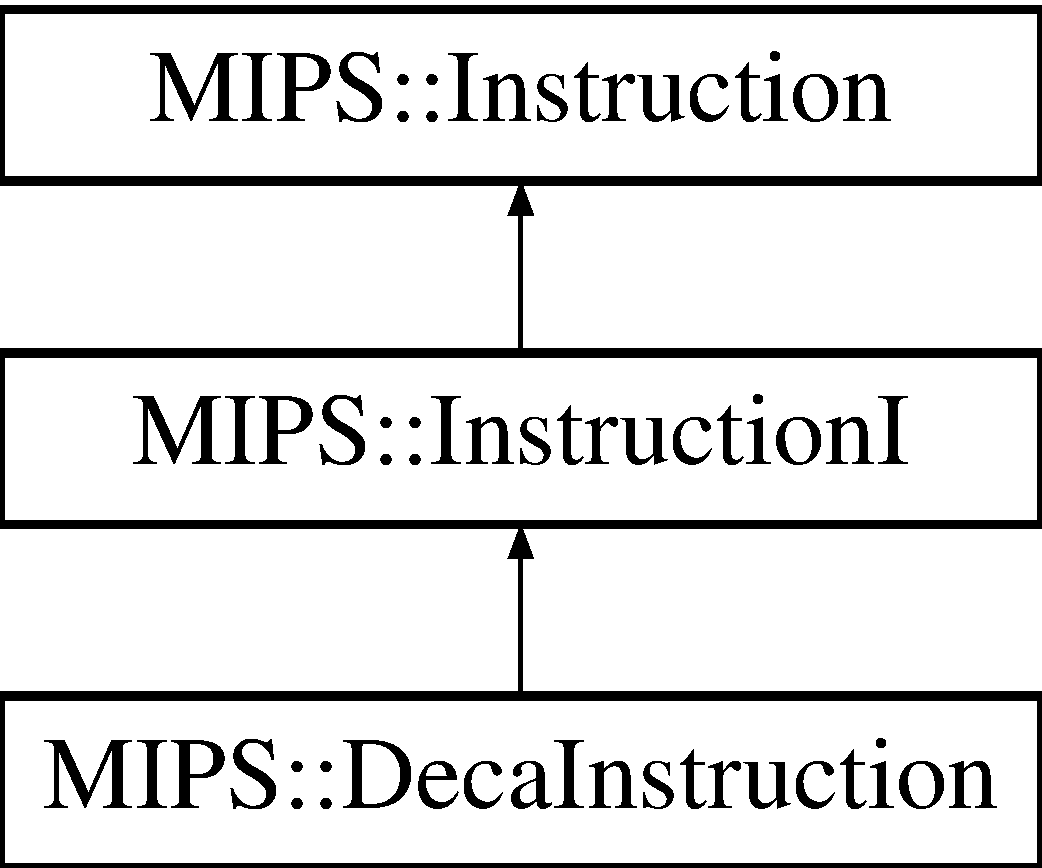
\includegraphics[height=3.000000cm]{classMIPS_1_1DecaInstruction}
\end{center}
\end{figure}
\subsection*{Public Member Functions}
\begin{DoxyCompactItemize}
\item 
\hyperlink{classMIPS_1_1DecaInstruction_a12f8f1eb9e3cf3afd1a08353b55e2062}{Deca\+Instruction} (\hyperlink{core_8hpp_a6074bae122ae7b527864eec42c728c3c}{bit8\+\_\+t} \hyperlink{classMIPS_1_1Instruction_a45cc6808b5dde8a5d41067d148b55476}{opcode}, \hyperlink{classMIPS_1_1Register}{Register} $\ast$\hyperlink{classMIPS_1_1InstructionI_a2be191d5b3dce505e2e626ec02eb4d62}{rs}, \hyperlink{classMIPS_1_1Register}{Register} $\ast$\hyperlink{classMIPS_1_1InstructionI_add1db07a5c954f35271de8c8a5737487}{rt}, \hyperlink{core_8hpp_a6074bae122ae7b527864eec42c728c3c}{bit8\+\_\+t} \hyperlink{classMIPS_1_1InstructionI_aa9b6da37c374c2ec8d96448d341e5e7d}{shamt}, \hyperlink{core_8hpp_a6074bae122ae7b527864eec42c728c3c}{bit8\+\_\+t} \hyperlink{classMIPS_1_1InstructionI_a5c6efcbbd233a7447c1fe24ea0a1e558}{funct})
\item 
\hyperlink{core_8hpp_adc265a970bc35995b5879784bbb3f1b7}{bit16\+\_\+t} \hyperlink{classMIPS_1_1DecaInstruction_a82c3d685d910d2c52163f5faa1750aca}{execute} ()
\end{DoxyCompactItemize}
\subsection*{Additional Inherited Members}


\subsection{Detailed Description}
Classe que faz a operação de D\+E\+CA no processador.

\begin{DoxyAuthor}{Author}
Felipe Dias 
\end{DoxyAuthor}


\subsection{Constructor \& Destructor Documentation}
\index{M\+I\+P\+S\+::\+Deca\+Instruction@{M\+I\+P\+S\+::\+Deca\+Instruction}!Deca\+Instruction@{Deca\+Instruction}}
\index{Deca\+Instruction@{Deca\+Instruction}!M\+I\+P\+S\+::\+Deca\+Instruction@{M\+I\+P\+S\+::\+Deca\+Instruction}}
\subsubsection[{\texorpdfstring{Deca\+Instruction(bit8\+\_\+t opcode, Register $\ast$rs, Register $\ast$rt, bit8\+\_\+t shamt, bit8\+\_\+t funct)}{DecaInstruction(bit8_t opcode, Register *rs, Register *rt, bit8_t shamt, bit8_t funct)}}]{\setlength{\rightskip}{0pt plus 5cm}M\+I\+P\+S\+::\+Deca\+Instruction\+::\+Deca\+Instruction (
\begin{DoxyParamCaption}
\item[{{\bf bit8\+\_\+t}}]{opcode, }
\item[{{\bf Register} $\ast$}]{rs, }
\item[{{\bf Register} $\ast$}]{rt, }
\item[{{\bf bit8\+\_\+t}}]{shamt, }
\item[{{\bf bit8\+\_\+t}}]{funct}
\end{DoxyParamCaption}
)\hspace{0.3cm}{\ttfamily [inline]}}\hypertarget{classMIPS_1_1DecaInstruction_a12f8f1eb9e3cf3afd1a08353b55e2062}{}\label{classMIPS_1_1DecaInstruction_a12f8f1eb9e3cf3afd1a08353b55e2062}
Constroi uma nova instrução. 

\subsection{Member Function Documentation}
\index{M\+I\+P\+S\+::\+Deca\+Instruction@{M\+I\+P\+S\+::\+Deca\+Instruction}!execute@{execute}}
\index{execute@{execute}!M\+I\+P\+S\+::\+Deca\+Instruction@{M\+I\+P\+S\+::\+Deca\+Instruction}}
\subsubsection[{\texorpdfstring{execute()}{execute()}}]{\setlength{\rightskip}{0pt plus 5cm}{\bf bit16\+\_\+t} M\+I\+P\+S\+::\+Deca\+Instruction\+::execute (
\begin{DoxyParamCaption}
{}
\end{DoxyParamCaption}
)\hspace{0.3cm}{\ttfamily [virtual]}}\hypertarget{classMIPS_1_1DecaInstruction_a82c3d685d910d2c52163f5faa1750aca}{}\label{classMIPS_1_1DecaInstruction_a82c3d685d910d2c52163f5faa1750aca}
Função que executa a operação de decremento.

\begin{DoxyReturn}{Returns}
resultado da operação 
\end{DoxyReturn}


Implements \hyperlink{classMIPS_1_1InstructionI_ae60fca5801bf5415cdff06d2aa11764f}{M\+I\+P\+S\+::\+InstructionI}.



The documentation for this class was generated from the following file\+:\begin{DoxyCompactItemize}
\item 
include/mips/instructions/format\+\_\+\+I/deca.\+hpp\end{DoxyCompactItemize}

\hypertarget{classMIPS_1_1Encoder}{}\section{M\+I\+PS\+:\+:Encoder Class Reference}
\label{classMIPS_1_1Encoder}\index{M\+I\+P\+S\+::\+Encoder@{M\+I\+P\+S\+::\+Encoder}}


{\ttfamily \#include $<$encoder.\+hpp$>$}

Inheritance diagram for M\+I\+PS\+:\+:Encoder\+:\begin{figure}[H]
\begin{center}
\leavevmode
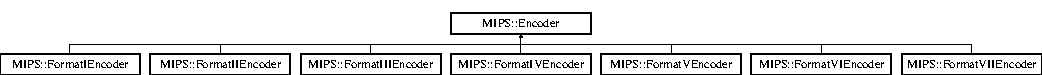
\includegraphics[height=1.012658cm]{classMIPS_1_1Encoder}
\end{center}
\end{figure}
\subsection*{Public Member Functions}
\begin{DoxyCompactItemize}
\item 
\hyperlink{classMIPS_1_1Encoder_a8c8b884b1cab08714cea0e467a5bea97}{Encoder} ()
\item 
virtual \hyperlink{classMIPS_1_1Encoder_aa19e1b31786eef05c8633790a12fa2a2}{$\sim$\+Encoder} ()
\item 
virtual \hyperlink{core_8hpp_aa514fd240a0e29abb2a2e4c805d7f1a4}{instruction\+\_\+t} \hyperlink{classMIPS_1_1Encoder_ac3ea6ce91eabd41b3c512a39ee4c3550}{encode} ()=0
\item 
virtual void \hyperlink{classMIPS_1_1Encoder_a4a29c42d601460be8e8d353d8fc0da34}{parse} (std\+::vector$<$ char $\ast$ $>$ \&params)=0
\end{DoxyCompactItemize}
\subsection*{Protected Member Functions}
\begin{DoxyCompactItemize}
\item 
\hyperlink{core_8hpp_a6074bae122ae7b527864eec42c728c3c}{bit8\+\_\+t} \hyperlink{classMIPS_1_1Encoder_af0e5dea3612f5063e48257bf0028f2dd}{get\+Register\+Number} (const char $\ast$name)
\end{DoxyCompactItemize}
\subsection*{Protected Attributes}
\begin{DoxyCompactItemize}
\item 
\hyperlink{core_8hpp_a6074bae122ae7b527864eec42c728c3c}{bit8\+\_\+t} \hyperlink{classMIPS_1_1Encoder_a1d07a78c088f8180af5f7b9ec3ca10f0}{opcode}
\end{DoxyCompactItemize}


\subsection{Detailed Description}
Classe abstrata que cria uma interface para todos os codificadores de instruções M\+I\+PS 32.

\begin{DoxyAuthor}{Author}
Matheus Nogueira 
\end{DoxyAuthor}


\subsection{Constructor \& Destructor Documentation}
\index{M\+I\+P\+S\+::\+Encoder@{M\+I\+P\+S\+::\+Encoder}!Encoder@{Encoder}}
\index{Encoder@{Encoder}!M\+I\+P\+S\+::\+Encoder@{M\+I\+P\+S\+::\+Encoder}}
\subsubsection[{\texorpdfstring{Encoder()}{Encoder()}}]{\setlength{\rightskip}{0pt plus 5cm}M\+I\+P\+S\+::\+Encoder\+::\+Encoder (
\begin{DoxyParamCaption}
{}
\end{DoxyParamCaption}
)}\hypertarget{classMIPS_1_1Encoder_a8c8b884b1cab08714cea0e467a5bea97}{}\label{classMIPS_1_1Encoder_a8c8b884b1cab08714cea0e467a5bea97}
Cria um novo codificador.


\begin{DoxyParams}{Parameters}
{\em labels} & tabela de labels extraídos do código. \\
\hline
{\em type} & tipo de codificador. \\
\hline
\end{DoxyParams}
\index{M\+I\+P\+S\+::\+Encoder@{M\+I\+P\+S\+::\+Encoder}!````~Encoder@{$\sim$\+Encoder}}
\index{````~Encoder@{$\sim$\+Encoder}!M\+I\+P\+S\+::\+Encoder@{M\+I\+P\+S\+::\+Encoder}}
\subsubsection[{\texorpdfstring{$\sim$\+Encoder()}{~Encoder()}}]{\setlength{\rightskip}{0pt plus 5cm}virtual M\+I\+P\+S\+::\+Encoder\+::$\sim$\+Encoder (
\begin{DoxyParamCaption}
{}
\end{DoxyParamCaption}
)\hspace{0.3cm}{\ttfamily [inline]}, {\ttfamily [virtual]}}\hypertarget{classMIPS_1_1Encoder_aa19e1b31786eef05c8633790a12fa2a2}{}\label{classMIPS_1_1Encoder_aa19e1b31786eef05c8633790a12fa2a2}
Destroi o codificador. 

\subsection{Member Function Documentation}
\index{M\+I\+P\+S\+::\+Encoder@{M\+I\+P\+S\+::\+Encoder}!encode@{encode}}
\index{encode@{encode}!M\+I\+P\+S\+::\+Encoder@{M\+I\+P\+S\+::\+Encoder}}
\subsubsection[{\texorpdfstring{encode()=0}{encode()=0}}]{\setlength{\rightskip}{0pt plus 5cm}virtual {\bf instruction\+\_\+t} M\+I\+P\+S\+::\+Encoder\+::encode (
\begin{DoxyParamCaption}
{}
\end{DoxyParamCaption}
)\hspace{0.3cm}{\ttfamily [pure virtual]}}\hypertarget{classMIPS_1_1Encoder_ac3ea6ce91eabd41b3c512a39ee4c3550}{}\label{classMIPS_1_1Encoder_ac3ea6ce91eabd41b3c512a39ee4c3550}
Codifica a ultima instrução que foi analisada pelo parser do codificador.

\begin{DoxyReturn}{Returns}
instrução 16 bits. 
\end{DoxyReturn}


Implemented in \hyperlink{classMIPS_1_1FormatIEncoder_af9fcd414057f2c01f2dada479d8592cb}{M\+I\+P\+S\+::\+Format\+I\+Encoder}, \hyperlink{classMIPS_1_1FormatIIEncoder_aaf5f5f9d4c9b6b63b150b239cb5b03fe}{M\+I\+P\+S\+::\+Format\+I\+I\+Encoder}, \hyperlink{classMIPS_1_1FormatIIIEncoder_ab243fc73a602716a7ed15f13dbd2b695}{M\+I\+P\+S\+::\+Format\+I\+I\+I\+Encoder}, \hyperlink{classMIPS_1_1FormatIVEncoder_a1d23ca4c9c81536dd43a18dc8dd43f97}{M\+I\+P\+S\+::\+Format\+I\+V\+Encoder}, \hyperlink{classMIPS_1_1FormatVEncoder_a95e96820cef484d427c64145006d8837}{M\+I\+P\+S\+::\+Format\+V\+Encoder}, \hyperlink{classMIPS_1_1FormatVIEncoder_ae0a892a24d712d260f80dbc6e85b7090}{M\+I\+P\+S\+::\+Format\+V\+I\+Encoder}, and \hyperlink{classMIPS_1_1FormatVIIEncoder_a2afcc51d8983491e39d145766639b995}{M\+I\+P\+S\+::\+Format\+V\+I\+I\+Encoder}.

\index{M\+I\+P\+S\+::\+Encoder@{M\+I\+P\+S\+::\+Encoder}!get\+Register\+Number@{get\+Register\+Number}}
\index{get\+Register\+Number@{get\+Register\+Number}!M\+I\+P\+S\+::\+Encoder@{M\+I\+P\+S\+::\+Encoder}}
\subsubsection[{\texorpdfstring{get\+Register\+Number(const char $\ast$name)}{getRegisterNumber(const char *name)}}]{\setlength{\rightskip}{0pt plus 5cm}{\bf bit8\+\_\+t} M\+I\+P\+S\+::\+Encoder\+::get\+Register\+Number (
\begin{DoxyParamCaption}
\item[{const char $\ast$}]{name}
\end{DoxyParamCaption}
)\hspace{0.3cm}{\ttfamily [protected]}}\hypertarget{classMIPS_1_1Encoder_af0e5dea3612f5063e48257bf0028f2dd}{}\label{classMIPS_1_1Encoder_af0e5dea3612f5063e48257bf0028f2dd}
Retorna o número do registrador solicitado.


\begin{DoxyParams}{Parameters}
{\em name} & nome do registrador. \\
\hline
\end{DoxyParams}
\begin{DoxyReturn}{Returns}
número do registrador 
\end{DoxyReturn}
\index{M\+I\+P\+S\+::\+Encoder@{M\+I\+P\+S\+::\+Encoder}!parse@{parse}}
\index{parse@{parse}!M\+I\+P\+S\+::\+Encoder@{M\+I\+P\+S\+::\+Encoder}}
\subsubsection[{\texorpdfstring{parse(std\+::vector$<$ char $\ast$ $>$ \&params)=0}{parse(std::vector< char * > &params)=0}}]{\setlength{\rightskip}{0pt plus 5cm}virtual void M\+I\+P\+S\+::\+Encoder\+::parse (
\begin{DoxyParamCaption}
\item[{std\+::vector$<$ char $\ast$ $>$ \&}]{params}
\end{DoxyParamCaption}
)\hspace{0.3cm}{\ttfamily [pure virtual]}}\hypertarget{classMIPS_1_1Encoder_a4a29c42d601460be8e8d353d8fc0da34}{}\label{classMIPS_1_1Encoder_a4a29c42d601460be8e8d353d8fc0da34}
Percorre a instrução em assembly e extraí os dados dela para poder montar uma instrução binária.


\begin{DoxyParams}{Parameters}
{\em params} & parametros da instrução. \\
\hline
\end{DoxyParams}


Implemented in \hyperlink{classMIPS_1_1FormatIEncoder_a04b46dc7d7b3734e42eaeedc500de2da}{M\+I\+P\+S\+::\+Format\+I\+Encoder}, \hyperlink{classMIPS_1_1FormatIIEncoder_aa988c9638985b07eea58f3e11ff4c2e7}{M\+I\+P\+S\+::\+Format\+I\+I\+Encoder}, \hyperlink{classMIPS_1_1FormatIIIEncoder_a06c8d98fe19c20d5e4f0986d7d500637}{M\+I\+P\+S\+::\+Format\+I\+I\+I\+Encoder}, \hyperlink{classMIPS_1_1FormatIVEncoder_a42f251011a97af63a707b4d0607e18a9}{M\+I\+P\+S\+::\+Format\+I\+V\+Encoder}, \hyperlink{classMIPS_1_1FormatVEncoder_af73c15fbc94eac0f8b28e6d7fa2e4dc2}{M\+I\+P\+S\+::\+Format\+V\+Encoder}, \hyperlink{classMIPS_1_1FormatVIEncoder_a4cec696ab9deca5b957ddbab97139631}{M\+I\+P\+S\+::\+Format\+V\+I\+Encoder}, and \hyperlink{classMIPS_1_1FormatVIIEncoder_a67272c7aad39c6f49c4aa162119215ba}{M\+I\+P\+S\+::\+Format\+V\+I\+I\+Encoder}.



\subsection{Member Data Documentation}
\index{M\+I\+P\+S\+::\+Encoder@{M\+I\+P\+S\+::\+Encoder}!opcode@{opcode}}
\index{opcode@{opcode}!M\+I\+P\+S\+::\+Encoder@{M\+I\+P\+S\+::\+Encoder}}
\subsubsection[{\texorpdfstring{opcode}{opcode}}]{\setlength{\rightskip}{0pt plus 5cm}{\bf bit8\+\_\+t} M\+I\+P\+S\+::\+Encoder\+::opcode\hspace{0.3cm}{\ttfamily [protected]}}\hypertarget{classMIPS_1_1Encoder_a1d07a78c088f8180af5f7b9ec3ca10f0}{}\label{classMIPS_1_1Encoder_a1d07a78c088f8180af5f7b9ec3ca10f0}
Opcode da instrução. 

The documentation for this class was generated from the following file\+:\begin{DoxyCompactItemize}
\item 
include/mips/interpreter/encoder/\hyperlink{encoder_8hpp}{encoder.\+hpp}\end{DoxyCompactItemize}

\hypertarget{classMIPS_1_1EncoderFactory}{}\section{M\+I\+PS\+:\+:Encoder\+Factory Class Reference}
\label{classMIPS_1_1EncoderFactory}\index{M\+I\+P\+S\+::\+Encoder\+Factory@{M\+I\+P\+S\+::\+Encoder\+Factory}}


{\ttfamily \#include $<$encoder\+\_\+factory.\+hpp$>$}

\subsection*{Public Member Functions}
\begin{DoxyCompactItemize}
\item 
\hyperlink{classMIPS_1_1EncoderFactory_a2756a65d715e2f6ba953a6acc4ee95a8}{Encoder\+Factory} ()
\item 
\hyperlink{classMIPS_1_1Encoder}{Encoder} $\ast$ \hyperlink{classMIPS_1_1EncoderFactory_a38f2aab5758ae0fd464346a61924b853}{produce} (const char $\ast$instruction)
\end{DoxyCompactItemize}


\subsection{Detailed Description}
Fábrica responsável por referenciar os codificadores corretos para cada instrução da linguagem de montagem do micro-\/\+R\+I\+SC.

\begin{DoxyAuthor}{Author}
Matheus Nogueira 
\end{DoxyAuthor}


\subsection{Constructor \& Destructor Documentation}
\index{M\+I\+P\+S\+::\+Encoder\+Factory@{M\+I\+P\+S\+::\+Encoder\+Factory}!Encoder\+Factory@{Encoder\+Factory}}
\index{Encoder\+Factory@{Encoder\+Factory}!M\+I\+P\+S\+::\+Encoder\+Factory@{M\+I\+P\+S\+::\+Encoder\+Factory}}
\subsubsection[{\texorpdfstring{Encoder\+Factory()}{EncoderFactory()}}]{\setlength{\rightskip}{0pt plus 5cm}M\+I\+P\+S\+::\+Encoder\+Factory\+::\+Encoder\+Factory (
\begin{DoxyParamCaption}
{}
\end{DoxyParamCaption}
)\hspace{0.3cm}{\ttfamily [inline]}}\hypertarget{classMIPS_1_1EncoderFactory_a2756a65d715e2f6ba953a6acc4ee95a8}{}\label{classMIPS_1_1EncoderFactory_a2756a65d715e2f6ba953a6acc4ee95a8}
Cria uma nova fábrica de codificadores. 

\subsection{Member Function Documentation}
\index{M\+I\+P\+S\+::\+Encoder\+Factory@{M\+I\+P\+S\+::\+Encoder\+Factory}!produce@{produce}}
\index{produce@{produce}!M\+I\+P\+S\+::\+Encoder\+Factory@{M\+I\+P\+S\+::\+Encoder\+Factory}}
\subsubsection[{\texorpdfstring{produce(const char $\ast$instruction)}{produce(const char *instruction)}}]{\setlength{\rightskip}{0pt plus 5cm}{\bf Encoder}$\ast$ M\+I\+P\+S\+::\+Encoder\+Factory\+::produce (
\begin{DoxyParamCaption}
\item[{const char $\ast$}]{instruction}
\end{DoxyParamCaption}
)}\hypertarget{classMIPS_1_1EncoderFactory_a38f2aab5758ae0fd464346a61924b853}{}\label{classMIPS_1_1EncoderFactory_a38f2aab5758ae0fd464346a61924b853}
Produz um codificador para determinada instrução.


\begin{DoxyParams}{Parameters}
{\em instruction} & nome da instrução que deve ser codificada. \\
\hline
\end{DoxyParams}


The documentation for this class was generated from the following file\+:\begin{DoxyCompactItemize}
\item 
include/mips/interpreter/encoder/\hyperlink{encoder__factory_8hpp}{encoder\+\_\+factory.\+hpp}\end{DoxyCompactItemize}

\hypertarget{classMIPS_1_1Event}{}\section{M\+I\+PS\+:\+:Event Class Reference}
\label{classMIPS_1_1Event}\index{M\+I\+P\+S\+::\+Event@{M\+I\+P\+S\+::\+Event}}


{\ttfamily \#include $<$event.\+hpp$>$}

\subsection*{Public Member Functions}
\begin{DoxyCompactItemize}
\item 
\hyperlink{classMIPS_1_1Event_a3c66c10469c0675dba66809fe92ba165}{Event} (\hyperlink{event_8hpp_a2b933d1ba3dc5a595db4dfa5b049c78c}{Event\+Type} type, void $\ast$data, bool autodestroy=false)
\item 
virtual \hyperlink{classMIPS_1_1Event_ae6a30dc2280feb5f1ec745cea46555f1}{$\sim$\+Event} ()
\item 
bool \hyperlink{classMIPS_1_1Event_a744dd00b534097bcd4d5db327a9da85a}{should\+Destroy} ()
\end{DoxyCompactItemize}
\subsection*{Public Attributes}
\begin{DoxyCompactItemize}
\item 
const \hyperlink{event_8hpp_a2b933d1ba3dc5a595db4dfa5b049c78c}{Event\+Type} \hyperlink{classMIPS_1_1Event_ab726d36d16847f2b2250394c6a462655}{event\+\_\+type}
\item 
void $\ast$ \hyperlink{classMIPS_1_1Event_a66f2b7a25dfb644ad5dc5b074f4b41a0}{data\+\_\+ptr}
\end{DoxyCompactItemize}


\subsection{Detailed Description}
Classe responsável por representar um evento que pode ser despachado pelo despachante de eventos do emulador.

\begin{DoxyAuthor}{Author}
Matheus Nogueira 
\end{DoxyAuthor}


\subsection{Constructor \& Destructor Documentation}
\index{M\+I\+P\+S\+::\+Event@{M\+I\+P\+S\+::\+Event}!Event@{Event}}
\index{Event@{Event}!M\+I\+P\+S\+::\+Event@{M\+I\+P\+S\+::\+Event}}
\subsubsection[{\texorpdfstring{Event(\+Event\+Type type, void $\ast$data, bool autodestroy=false)}{Event(EventType type, void *data, bool autodestroy=false)}}]{\setlength{\rightskip}{0pt plus 5cm}M\+I\+P\+S\+::\+Event\+::\+Event (
\begin{DoxyParamCaption}
\item[{{\bf Event\+Type}}]{type, }
\item[{void $\ast$}]{data, }
\item[{bool}]{autodestroy = {\ttfamily false}}
\end{DoxyParamCaption}
)}\hypertarget{classMIPS_1_1Event_a3c66c10469c0675dba66809fe92ba165}{}\label{classMIPS_1_1Event_a3c66c10469c0675dba66809fe92ba165}
Cria um novo evento.


\begin{DoxyParams}{Parameters}
{\em type} & tipo do evento \\
\hline
{\em data} & dados associados ao evento. Esses dados associados devem ser alocados de forma dinâmica pelo programador, utilizando a função malloc. O despachante de eventos é responsável por destruir esses dados após seu uso caso a flag autodestroy seja ativada. \\
\hline
{\em autodestroy} & indica que os dados do evento devem ser destruídos após que o evento seja despachado para todos seus ouvintes. \\
\hline
\end{DoxyParams}
\index{M\+I\+P\+S\+::\+Event@{M\+I\+P\+S\+::\+Event}!````~Event@{$\sim$\+Event}}
\index{````~Event@{$\sim$\+Event}!M\+I\+P\+S\+::\+Event@{M\+I\+P\+S\+::\+Event}}
\subsubsection[{\texorpdfstring{$\sim$\+Event()}{~Event()}}]{\setlength{\rightskip}{0pt plus 5cm}virtual M\+I\+P\+S\+::\+Event\+::$\sim$\+Event (
\begin{DoxyParamCaption}
{}
\end{DoxyParamCaption}
)\hspace{0.3cm}{\ttfamily [virtual]}}\hypertarget{classMIPS_1_1Event_ae6a30dc2280feb5f1ec745cea46555f1}{}\label{classMIPS_1_1Event_ae6a30dc2280feb5f1ec745cea46555f1}
Destroi o evento e os dados relacionados ao mesmo. 

\subsection{Member Function Documentation}
\index{M\+I\+P\+S\+::\+Event@{M\+I\+P\+S\+::\+Event}!should\+Destroy@{should\+Destroy}}
\index{should\+Destroy@{should\+Destroy}!M\+I\+P\+S\+::\+Event@{M\+I\+P\+S\+::\+Event}}
\subsubsection[{\texorpdfstring{should\+Destroy()}{shouldDestroy()}}]{\setlength{\rightskip}{0pt plus 5cm}bool M\+I\+P\+S\+::\+Event\+::should\+Destroy (
\begin{DoxyParamCaption}
{}
\end{DoxyParamCaption}
)}\hypertarget{classMIPS_1_1Event_a744dd00b534097bcd4d5db327a9da85a}{}\label{classMIPS_1_1Event_a744dd00b534097bcd4d5db327a9da85a}
Verifica se o evento deve se auto destruir.

\begin{DoxyReturn}{Returns}
true se o evento deve se auto destruir. 
\end{DoxyReturn}


\subsection{Member Data Documentation}
\index{M\+I\+P\+S\+::\+Event@{M\+I\+P\+S\+::\+Event}!data\+\_\+ptr@{data\+\_\+ptr}}
\index{data\+\_\+ptr@{data\+\_\+ptr}!M\+I\+P\+S\+::\+Event@{M\+I\+P\+S\+::\+Event}}
\subsubsection[{\texorpdfstring{data\+\_\+ptr}{data_ptr}}]{\setlength{\rightskip}{0pt plus 5cm}void$\ast$ M\+I\+P\+S\+::\+Event\+::data\+\_\+ptr}\hypertarget{classMIPS_1_1Event_a66f2b7a25dfb644ad5dc5b074f4b41a0}{}\label{classMIPS_1_1Event_a66f2b7a25dfb644ad5dc5b074f4b41a0}
Ponteiro para os dados do evento. \index{M\+I\+P\+S\+::\+Event@{M\+I\+P\+S\+::\+Event}!event\+\_\+type@{event\+\_\+type}}
\index{event\+\_\+type@{event\+\_\+type}!M\+I\+P\+S\+::\+Event@{M\+I\+P\+S\+::\+Event}}
\subsubsection[{\texorpdfstring{event\+\_\+type}{event_type}}]{\setlength{\rightskip}{0pt plus 5cm}const {\bf Event\+Type} M\+I\+P\+S\+::\+Event\+::event\+\_\+type}\hypertarget{classMIPS_1_1Event_ab726d36d16847f2b2250394c6a462655}{}\label{classMIPS_1_1Event_ab726d36d16847f2b2250394c6a462655}
Tipo de evento. 

The documentation for this class was generated from the following file\+:\begin{DoxyCompactItemize}
\item 
include/mips/util/event/\hyperlink{event_8hpp}{event.\+hpp}\end{DoxyCompactItemize}

\hypertarget{classMIPS_1_1EventDispatcher}{}\section{M\+I\+PS\+:\+:Event\+Dispatcher Class Reference}
\label{classMIPS_1_1EventDispatcher}\index{M\+I\+P\+S\+::\+Event\+Dispatcher@{M\+I\+P\+S\+::\+Event\+Dispatcher}}


{\ttfamily \#include $<$event\+\_\+dispatcher.\+hpp$>$}

\subsection*{Classes}
\begin{DoxyCompactItemize}
\item 
struct \hyperlink{structMIPS_1_1EventDispatcher_1_1ListenerMap}{Listener\+Map}
\end{DoxyCompactItemize}
\subsection*{Public Member Functions}
\begin{DoxyCompactItemize}
\item 
\hyperlink{classMIPS_1_1EventDispatcher_ac0274686b219131fffa051f3877cf952}{Event\+Dispatcher} ()
\item 
virtual \hyperlink{classMIPS_1_1EventDispatcher_ac443528f78d0d446590e1d550a9ed41a}{$\sim$\+Event\+Dispatcher} ()
\item 
void \hyperlink{classMIPS_1_1EventDispatcher_a39eedeb6d95d5725a2608880b24ac5fc}{dispatch} (\hyperlink{classMIPS_1_1Event}{Event} \&event)
\item 
void \hyperlink{classMIPS_1_1EventDispatcher_a9e4615cf1c83a18a259b6f48756db486}{add\+Event\+Listener} (\hyperlink{classMIPS_1_1EventListener}{Event\+Listener} $\ast$listener, \hyperlink{event_8hpp_a2b933d1ba3dc5a595db4dfa5b049c78c}{Event\+Type} event)
\end{DoxyCompactItemize}


\subsection{Detailed Description}
Classe responsável por permitir que componentes do emulador possam se comunicar por troca de mensagens transmitidas por eventos.

\begin{DoxyAuthor}{Author}
Matheus Nogueira 
\end{DoxyAuthor}


\subsection{Constructor \& Destructor Documentation}
\index{M\+I\+P\+S\+::\+Event\+Dispatcher@{M\+I\+P\+S\+::\+Event\+Dispatcher}!Event\+Dispatcher@{Event\+Dispatcher}}
\index{Event\+Dispatcher@{Event\+Dispatcher}!M\+I\+P\+S\+::\+Event\+Dispatcher@{M\+I\+P\+S\+::\+Event\+Dispatcher}}
\subsubsection[{\texorpdfstring{Event\+Dispatcher()}{EventDispatcher()}}]{\setlength{\rightskip}{0pt plus 5cm}M\+I\+P\+S\+::\+Event\+Dispatcher\+::\+Event\+Dispatcher (
\begin{DoxyParamCaption}
{}
\end{DoxyParamCaption}
)}\hypertarget{classMIPS_1_1EventDispatcher_ac0274686b219131fffa051f3877cf952}{}\label{classMIPS_1_1EventDispatcher_ac0274686b219131fffa051f3877cf952}
Cria um novo despachante de eventos. \index{M\+I\+P\+S\+::\+Event\+Dispatcher@{M\+I\+P\+S\+::\+Event\+Dispatcher}!````~Event\+Dispatcher@{$\sim$\+Event\+Dispatcher}}
\index{````~Event\+Dispatcher@{$\sim$\+Event\+Dispatcher}!M\+I\+P\+S\+::\+Event\+Dispatcher@{M\+I\+P\+S\+::\+Event\+Dispatcher}}
\subsubsection[{\texorpdfstring{$\sim$\+Event\+Dispatcher()}{~EventDispatcher()}}]{\setlength{\rightskip}{0pt plus 5cm}virtual M\+I\+P\+S\+::\+Event\+Dispatcher\+::$\sim$\+Event\+Dispatcher (
\begin{DoxyParamCaption}
{}
\end{DoxyParamCaption}
)\hspace{0.3cm}{\ttfamily [virtual]}}\hypertarget{classMIPS_1_1EventDispatcher_ac443528f78d0d446590e1d550a9ed41a}{}\label{classMIPS_1_1EventDispatcher_ac443528f78d0d446590e1d550a9ed41a}
Destroi o despachante de eventos. 

\subsection{Member Function Documentation}
\index{M\+I\+P\+S\+::\+Event\+Dispatcher@{M\+I\+P\+S\+::\+Event\+Dispatcher}!add\+Event\+Listener@{add\+Event\+Listener}}
\index{add\+Event\+Listener@{add\+Event\+Listener}!M\+I\+P\+S\+::\+Event\+Dispatcher@{M\+I\+P\+S\+::\+Event\+Dispatcher}}
\subsubsection[{\texorpdfstring{add\+Event\+Listener(\+Event\+Listener $\ast$listener, Event\+Type event)}{addEventListener(EventListener *listener, EventType event)}}]{\setlength{\rightskip}{0pt plus 5cm}void M\+I\+P\+S\+::\+Event\+Dispatcher\+::add\+Event\+Listener (
\begin{DoxyParamCaption}
\item[{{\bf Event\+Listener} $\ast$}]{listener, }
\item[{{\bf Event\+Type}}]{event}
\end{DoxyParamCaption}
)}\hypertarget{classMIPS_1_1EventDispatcher_a9e4615cf1c83a18a259b6f48756db486}{}\label{classMIPS_1_1EventDispatcher_a9e4615cf1c83a18a259b6f48756db486}
Adiciona um ouvinte de eventos nesse despachante.


\begin{DoxyParams}{Parameters}
{\em listener} & ouvinte de eventos \\
\hline
{\em event} & tipo de evento que o ouvinte irá escutar. \\
\hline
\end{DoxyParams}
\index{M\+I\+P\+S\+::\+Event\+Dispatcher@{M\+I\+P\+S\+::\+Event\+Dispatcher}!dispatch@{dispatch}}
\index{dispatch@{dispatch}!M\+I\+P\+S\+::\+Event\+Dispatcher@{M\+I\+P\+S\+::\+Event\+Dispatcher}}
\subsubsection[{\texorpdfstring{dispatch(\+Event \&event)}{dispatch(Event &event)}}]{\setlength{\rightskip}{0pt plus 5cm}void M\+I\+P\+S\+::\+Event\+Dispatcher\+::dispatch (
\begin{DoxyParamCaption}
\item[{{\bf Event} \&}]{event}
\end{DoxyParamCaption}
)}\hypertarget{classMIPS_1_1EventDispatcher_a39eedeb6d95d5725a2608880b24ac5fc}{}\label{classMIPS_1_1EventDispatcher_a39eedeb6d95d5725a2608880b24ac5fc}
Despacha um evento para todos os seus ouvintes. Caso o evento esteja marcado com a flag autodestroy, o evento será destruido logo após a chamada desse método.


\begin{DoxyParams}{Parameters}
{\em event} & evento a ser despachado. \\
\hline
\end{DoxyParams}


The documentation for this class was generated from the following file\+:\begin{DoxyCompactItemize}
\item 
include/mips/util/event/\hyperlink{event__dispatcher_8hpp}{event\+\_\+dispatcher.\+hpp}\end{DoxyCompactItemize}

\hypertarget{classMIPS_1_1EventListener}{}\section{M\+I\+PS\+:\+:Event\+Listener Class Reference}
\label{classMIPS_1_1EventListener}\index{M\+I\+P\+S\+::\+Event\+Listener@{M\+I\+P\+S\+::\+Event\+Listener}}


{\ttfamily \#include $<$event\+\_\+listener.\+hpp$>$}

\subsection*{Public Member Functions}
\begin{DoxyCompactItemize}
\item 
virtual void \hyperlink{classMIPS_1_1EventListener_adef11b7803496c63d344960e2952a997}{notify} (\hyperlink{classMIPS_1_1Event}{Event} \&event)
\end{DoxyCompactItemize}


\subsection{Detailed Description}
Classe abstrata que permite um objeto ouvir eventos vindos de outra classe.

\begin{DoxyAuthor}{Author}
Matheus Nogueira 
\end{DoxyAuthor}


\subsection{Member Function Documentation}
\index{M\+I\+P\+S\+::\+Event\+Listener@{M\+I\+P\+S\+::\+Event\+Listener}!notify@{notify}}
\index{notify@{notify}!M\+I\+P\+S\+::\+Event\+Listener@{M\+I\+P\+S\+::\+Event\+Listener}}
\subsubsection[{\texorpdfstring{notify(\+Event \&event)}{notify(Event &event)}}]{\setlength{\rightskip}{0pt plus 5cm}virtual void M\+I\+P\+S\+::\+Event\+Listener\+::notify (
\begin{DoxyParamCaption}
\item[{{\bf Event} \&}]{event}
\end{DoxyParamCaption}
)\hspace{0.3cm}{\ttfamily [virtual]}}\hypertarget{classMIPS_1_1EventListener_adef11b7803496c63d344960e2952a997}{}\label{classMIPS_1_1EventListener_adef11b7803496c63d344960e2952a997}
Função utilizada para notificar o objeto que algum evento o qual ele está esperando, ocorreu.


\begin{DoxyParams}{Parameters}
{\em event} & evento que ocorreu. \\
\hline
\end{DoxyParams}


The documentation for this class was generated from the following file\+:\begin{DoxyCompactItemize}
\item 
include/mips/util/event/\hyperlink{event__listener_8hpp}{event\+\_\+listener.\+hpp}\end{DoxyCompactItemize}

\hypertarget{classMIPS_1_1FileReader}{}\section{M\+I\+PS\+:\+:File\+Reader Class Reference}
\label{classMIPS_1_1FileReader}\index{M\+I\+P\+S\+::\+File\+Reader@{M\+I\+P\+S\+::\+File\+Reader}}


{\ttfamily \#include $<$file\+\_\+reader.\+hpp$>$}

\subsection*{Public Member Functions}
\begin{DoxyCompactItemize}
\item 
\hyperlink{classMIPS_1_1FileReader_ab3287e189c99bc1c6232e0a874824a04}{File\+Reader} (const char $\ast$filename)
\item 
\hyperlink{classMIPS_1_1FileReader_a9151c88a7f99aeddb7f2114b1263ccda}{File\+Reader} (const char $\ast$filename, \hyperlink{classMIPS_1_1Filter}{Filter} \&filter)
\item 
\hyperlink{classMIPS_1_1FileReader_a2357f2ae095cb728bfccf5d3b72529a8}{$\sim$\+File\+Reader} ()
\item 
char $\ast$ \hyperlink{classMIPS_1_1FileReader_af343e2652200f0ae52cedbfe22dba0cf}{next} ()
\item 
void \hyperlink{classMIPS_1_1FileReader_a5f60a3cdab4475ddf28bb3cc77a742ad}{rewind} ()
\item 
bool \hyperlink{classMIPS_1_1FileReader_a15e77fbddc428aaab28d750bdd777479}{has\+Next} ()
\end{DoxyCompactItemize}


\subsection{Detailed Description}
Classe responsável por ler o conteúdo de um arquivo e salvá-\/lo internamente, fazendo com que seja simples para obter as informações do mesmo.

\begin{DoxyAuthor}{Author}
Matheus Nogueira 
\end{DoxyAuthor}


\subsection{Constructor \& Destructor Documentation}
\index{M\+I\+P\+S\+::\+File\+Reader@{M\+I\+P\+S\+::\+File\+Reader}!File\+Reader@{File\+Reader}}
\index{File\+Reader@{File\+Reader}!M\+I\+P\+S\+::\+File\+Reader@{M\+I\+P\+S\+::\+File\+Reader}}
\subsubsection[{\texorpdfstring{File\+Reader(const char $\ast$filename)}{FileReader(const char *filename)}}]{\setlength{\rightskip}{0pt plus 5cm}M\+I\+P\+S\+::\+File\+Reader\+::\+File\+Reader (
\begin{DoxyParamCaption}
\item[{const char $\ast$}]{filename}
\end{DoxyParamCaption}
)}\hypertarget{classMIPS_1_1FileReader_ab3287e189c99bc1c6232e0a874824a04}{}\label{classMIPS_1_1FileReader_ab3287e189c99bc1c6232e0a874824a04}
Cria um novo leitor de arquivo.


\begin{DoxyParams}{Parameters}
{\em filename} & nome do arquivo a ser lido. \\
\hline
\end{DoxyParams}
\index{M\+I\+P\+S\+::\+File\+Reader@{M\+I\+P\+S\+::\+File\+Reader}!File\+Reader@{File\+Reader}}
\index{File\+Reader@{File\+Reader}!M\+I\+P\+S\+::\+File\+Reader@{M\+I\+P\+S\+::\+File\+Reader}}
\subsubsection[{\texorpdfstring{File\+Reader(const char $\ast$filename, Filter \&filter)}{FileReader(const char *filename, Filter &filter)}}]{\setlength{\rightskip}{0pt plus 5cm}M\+I\+P\+S\+::\+File\+Reader\+::\+File\+Reader (
\begin{DoxyParamCaption}
\item[{const char $\ast$}]{filename, }
\item[{{\bf Filter} \&}]{filter}
\end{DoxyParamCaption}
)}\hypertarget{classMIPS_1_1FileReader_a9151c88a7f99aeddb7f2114b1263ccda}{}\label{classMIPS_1_1FileReader_a9151c88a7f99aeddb7f2114b1263ccda}
Cria um novo leitor de arquivo que filtra determinadas entradas.


\begin{DoxyParams}{Parameters}
{\em filename} & nome do arquivo a ser lido. \\
\hline
{\em filter} & filtro a ser utilizado. \\
\hline
\end{DoxyParams}
\index{M\+I\+P\+S\+::\+File\+Reader@{M\+I\+P\+S\+::\+File\+Reader}!````~File\+Reader@{$\sim$\+File\+Reader}}
\index{````~File\+Reader@{$\sim$\+File\+Reader}!M\+I\+P\+S\+::\+File\+Reader@{M\+I\+P\+S\+::\+File\+Reader}}
\subsubsection[{\texorpdfstring{$\sim$\+File\+Reader()}{~FileReader()}}]{\setlength{\rightskip}{0pt plus 5cm}M\+I\+P\+S\+::\+File\+Reader\+::$\sim$\+File\+Reader (
\begin{DoxyParamCaption}
{}
\end{DoxyParamCaption}
)}\hypertarget{classMIPS_1_1FileReader_a2357f2ae095cb728bfccf5d3b72529a8}{}\label{classMIPS_1_1FileReader_a2357f2ae095cb728bfccf5d3b72529a8}
Destroi o leitor de arquivo e o conteúdo do buffer interno. 

\subsection{Member Function Documentation}
\index{M\+I\+P\+S\+::\+File\+Reader@{M\+I\+P\+S\+::\+File\+Reader}!has\+Next@{has\+Next}}
\index{has\+Next@{has\+Next}!M\+I\+P\+S\+::\+File\+Reader@{M\+I\+P\+S\+::\+File\+Reader}}
\subsubsection[{\texorpdfstring{has\+Next()}{hasNext()}}]{\setlength{\rightskip}{0pt plus 5cm}bool M\+I\+P\+S\+::\+File\+Reader\+::has\+Next (
\begin{DoxyParamCaption}
{}
\end{DoxyParamCaption}
)}\hypertarget{classMIPS_1_1FileReader_a15e77fbddc428aaab28d750bdd777479}{}\label{classMIPS_1_1FileReader_a15e77fbddc428aaab28d750bdd777479}
Checa se o arquivo ainda tem conteúdo para ser lido.

\begin{DoxyReturn}{Returns}
booleano que se true, indica que ainda existe linhas a ser lidas. 
\end{DoxyReturn}
\index{M\+I\+P\+S\+::\+File\+Reader@{M\+I\+P\+S\+::\+File\+Reader}!next@{next}}
\index{next@{next}!M\+I\+P\+S\+::\+File\+Reader@{M\+I\+P\+S\+::\+File\+Reader}}
\subsubsection[{\texorpdfstring{next()}{next()}}]{\setlength{\rightskip}{0pt plus 5cm}char$\ast$ M\+I\+P\+S\+::\+File\+Reader\+::next (
\begin{DoxyParamCaption}
{}
\end{DoxyParamCaption}
)}\hypertarget{classMIPS_1_1FileReader_af343e2652200f0ae52cedbfe22dba0cf}{}\label{classMIPS_1_1FileReader_af343e2652200f0ae52cedbfe22dba0cf}
Retorna a proxima linha do arquivo.

\begin{DoxyReturn}{Returns}
proxima linha do arquivo. 
\end{DoxyReturn}
\index{M\+I\+P\+S\+::\+File\+Reader@{M\+I\+P\+S\+::\+File\+Reader}!rewind@{rewind}}
\index{rewind@{rewind}!M\+I\+P\+S\+::\+File\+Reader@{M\+I\+P\+S\+::\+File\+Reader}}
\subsubsection[{\texorpdfstring{rewind()}{rewind()}}]{\setlength{\rightskip}{0pt plus 5cm}void M\+I\+P\+S\+::\+File\+Reader\+::rewind (
\begin{DoxyParamCaption}
{}
\end{DoxyParamCaption}
)}\hypertarget{classMIPS_1_1FileReader_a5f60a3cdab4475ddf28bb3cc77a742ad}{}\label{classMIPS_1_1FileReader_a5f60a3cdab4475ddf28bb3cc77a742ad}
Retorna o ponteiro da linha atual para o inicio do arquivo. 

The documentation for this class was generated from the following file\+:\begin{DoxyCompactItemize}
\item 
include/mips/util/\hyperlink{file__reader_8hpp}{file\+\_\+reader.\+hpp}\end{DoxyCompactItemize}

\hypertarget{classMIPS_1_1Filter}{}\section{M\+I\+PS\+:\+:Filter Class Reference}
\label{classMIPS_1_1Filter}\index{M\+I\+P\+S\+::\+Filter@{M\+I\+P\+S\+::\+Filter}}


{\ttfamily \#include $<$filter.\+hpp$>$}

Inheritance diagram for M\+I\+PS\+:\+:Filter\+:\begin{figure}[H]
\begin{center}
\leavevmode
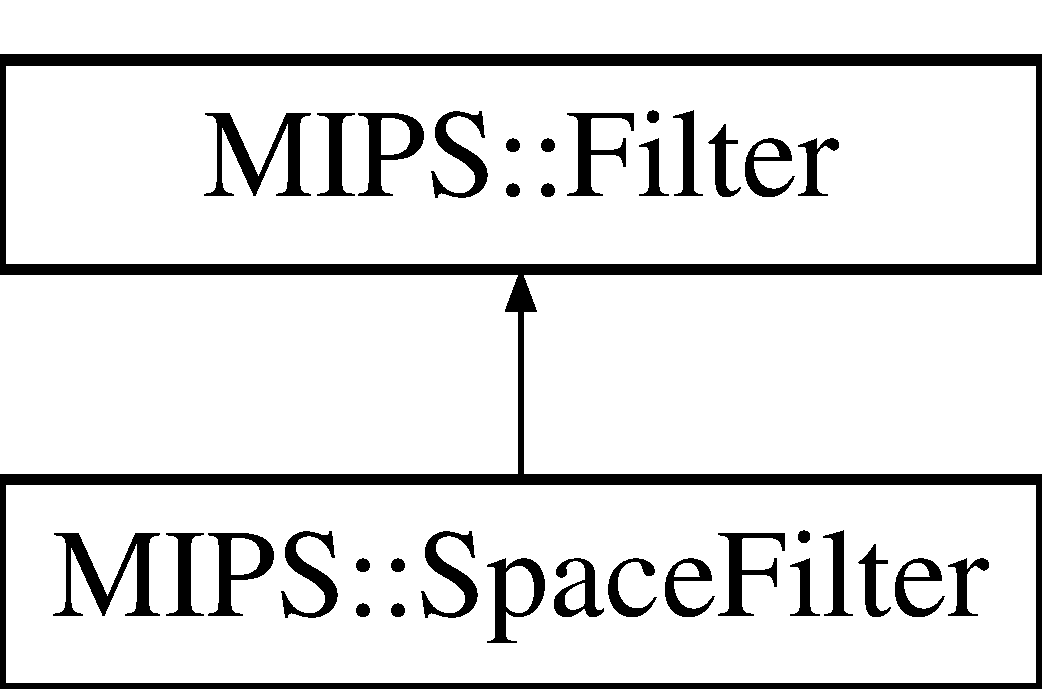
\includegraphics[height=2.000000cm]{classMIPS_1_1Filter}
\end{center}
\end{figure}
\subsection*{Public Member Functions}
\begin{DoxyCompactItemize}
\item 
virtual std\+::string \hyperlink{classMIPS_1_1Filter_a752c258e9d4090dd774fa4e829c95ae1}{filter} (std\+::string \&input)=0
\end{DoxyCompactItemize}


\subsection{Detailed Description}
Classe abstrata que representa um filtro de texto.

\begin{DoxyAuthor}{Author}
Matheus Nogueira 
\end{DoxyAuthor}


\subsection{Member Function Documentation}
\index{M\+I\+P\+S\+::\+Filter@{M\+I\+P\+S\+::\+Filter}!filter@{filter}}
\index{filter@{filter}!M\+I\+P\+S\+::\+Filter@{M\+I\+P\+S\+::\+Filter}}
\subsubsection[{\texorpdfstring{filter(std\+::string \&input)=0}{filter(std::string &input)=0}}]{\setlength{\rightskip}{0pt plus 5cm}virtual std\+::string M\+I\+P\+S\+::\+Filter\+::filter (
\begin{DoxyParamCaption}
\item[{std\+::string \&}]{input}
\end{DoxyParamCaption}
)\hspace{0.3cm}{\ttfamily [pure virtual]}}\hypertarget{classMIPS_1_1Filter_a752c258e9d4090dd774fa4e829c95ae1}{}\label{classMIPS_1_1Filter_a752c258e9d4090dd774fa4e829c95ae1}
Filtra uma string e retorna uma nova instância da mesma.


\begin{DoxyParams}{Parameters}
{\em input} & string a ser filtrada. \\
\hline
\end{DoxyParams}
\begin{DoxyReturn}{Returns}
string filtrada. 
\end{DoxyReturn}


Implemented in \hyperlink{classMIPS_1_1SpaceFilter_af6182f9ed8fb061e3ab9d7b437234952}{M\+I\+P\+S\+::\+Space\+Filter}.



The documentation for this class was generated from the following file\+:\begin{DoxyCompactItemize}
\item 
include/mips/util/filter/\hyperlink{filter_8hpp}{filter.\+hpp}\end{DoxyCompactItemize}

\hypertarget{classMIPS_1_1FormatIEncoder}{}\section{M\+I\+PS\+:\+:Format\+I\+Encoder Class Reference}
\label{classMIPS_1_1FormatIEncoder}\index{M\+I\+P\+S\+::\+Format\+I\+Encoder@{M\+I\+P\+S\+::\+Format\+I\+Encoder}}


{\ttfamily \#include $<$format\+\_\+\+I\+\_\+encoder.\+hpp$>$}

Inheritance diagram for M\+I\+PS\+:\+:Format\+I\+Encoder\+:\begin{figure}[H]
\begin{center}
\leavevmode
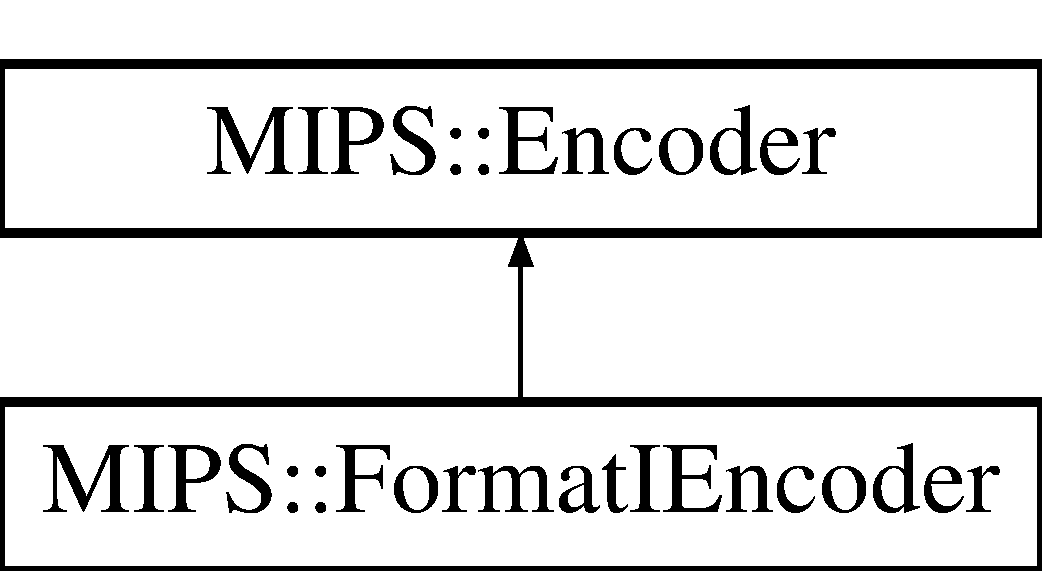
\includegraphics[height=2.000000cm]{classMIPS_1_1FormatIEncoder}
\end{center}
\end{figure}
\subsection*{Public Member Functions}
\begin{DoxyCompactItemize}
\item 
\hyperlink{core_8hpp_aa514fd240a0e29abb2a2e4c805d7f1a4}{instruction\+\_\+t} \hyperlink{classMIPS_1_1FormatIEncoder_af9fcd414057f2c01f2dada479d8592cb}{encode} ()
\item 
void \hyperlink{classMIPS_1_1FormatIEncoder_a04b46dc7d7b3734e42eaeedc500de2da}{parse} (std\+::vector$<$ char $\ast$ $>$ \&params)
\end{DoxyCompactItemize}
\subsection*{Additional Inherited Members}


\subsection{Detailed Description}
Codificador responsável por transformar uma instrução assembly em uma instrução binária, seguindo o formato de instrução no formato I.

\begin{DoxyAuthor}{Author}
Matheus Nogueira 
\end{DoxyAuthor}


\subsection{Member Function Documentation}
\index{M\+I\+P\+S\+::\+Format\+I\+Encoder@{M\+I\+P\+S\+::\+Format\+I\+Encoder}!encode@{encode}}
\index{encode@{encode}!M\+I\+P\+S\+::\+Format\+I\+Encoder@{M\+I\+P\+S\+::\+Format\+I\+Encoder}}
\subsubsection[{\texorpdfstring{encode()}{encode()}}]{\setlength{\rightskip}{0pt plus 5cm}{\bf instruction\+\_\+t} M\+I\+P\+S\+::\+Format\+I\+Encoder\+::encode (
\begin{DoxyParamCaption}
{}
\end{DoxyParamCaption}
)\hspace{0.3cm}{\ttfamily [virtual]}}\hypertarget{classMIPS_1_1FormatIEncoder_af9fcd414057f2c01f2dada479d8592cb}{}\label{classMIPS_1_1FormatIEncoder_af9fcd414057f2c01f2dada479d8592cb}
Codifica uma instrução assembly do formato I para uma instrução binária.

\begin{DoxyReturn}{Returns}
instrução binária de 16 bits 
\end{DoxyReturn}


Implements \hyperlink{classMIPS_1_1Encoder_ac3ea6ce91eabd41b3c512a39ee4c3550}{M\+I\+P\+S\+::\+Encoder}.

\index{M\+I\+P\+S\+::\+Format\+I\+Encoder@{M\+I\+P\+S\+::\+Format\+I\+Encoder}!parse@{parse}}
\index{parse@{parse}!M\+I\+P\+S\+::\+Format\+I\+Encoder@{M\+I\+P\+S\+::\+Format\+I\+Encoder}}
\subsubsection[{\texorpdfstring{parse(std\+::vector$<$ char $\ast$ $>$ \&params)}{parse(std::vector< char * > &params)}}]{\setlength{\rightskip}{0pt plus 5cm}void M\+I\+P\+S\+::\+Format\+I\+Encoder\+::parse (
\begin{DoxyParamCaption}
\item[{std\+::vector$<$ char $\ast$ $>$ \&}]{params}
\end{DoxyParamCaption}
)\hspace{0.3cm}{\ttfamily [virtual]}}\hypertarget{classMIPS_1_1FormatIEncoder_a04b46dc7d7b3734e42eaeedc500de2da}{}\label{classMIPS_1_1FormatIEncoder_a04b46dc7d7b3734e42eaeedc500de2da}
Realiza uma varredura na instrução assembly e define seus campos binários.


\begin{DoxyParams}{Parameters}
{\em params} & vector de parâmetros da instrução \\
\hline
\end{DoxyParams}


Implements \hyperlink{classMIPS_1_1Encoder_a4a29c42d601460be8e8d353d8fc0da34}{M\+I\+P\+S\+::\+Encoder}.



The documentation for this class was generated from the following file\+:\begin{DoxyCompactItemize}
\item 
include/mips/interpreter/encoder/\hyperlink{format__I__encoder_8hpp}{format\+\_\+\+I\+\_\+encoder.\+hpp}\end{DoxyCompactItemize}

\hypertarget{classMIPS_1_1FormatIIEncoder}{}\section{M\+I\+PS\+:\+:Format\+I\+I\+Encoder Class Reference}
\label{classMIPS_1_1FormatIIEncoder}\index{M\+I\+P\+S\+::\+Format\+I\+I\+Encoder@{M\+I\+P\+S\+::\+Format\+I\+I\+Encoder}}


{\ttfamily \#include $<$format\+\_\+\+I\+I\+\_\+encoder.\+hpp$>$}

Inheritance diagram for M\+I\+PS\+:\+:Format\+I\+I\+Encoder\+:\begin{figure}[H]
\begin{center}
\leavevmode
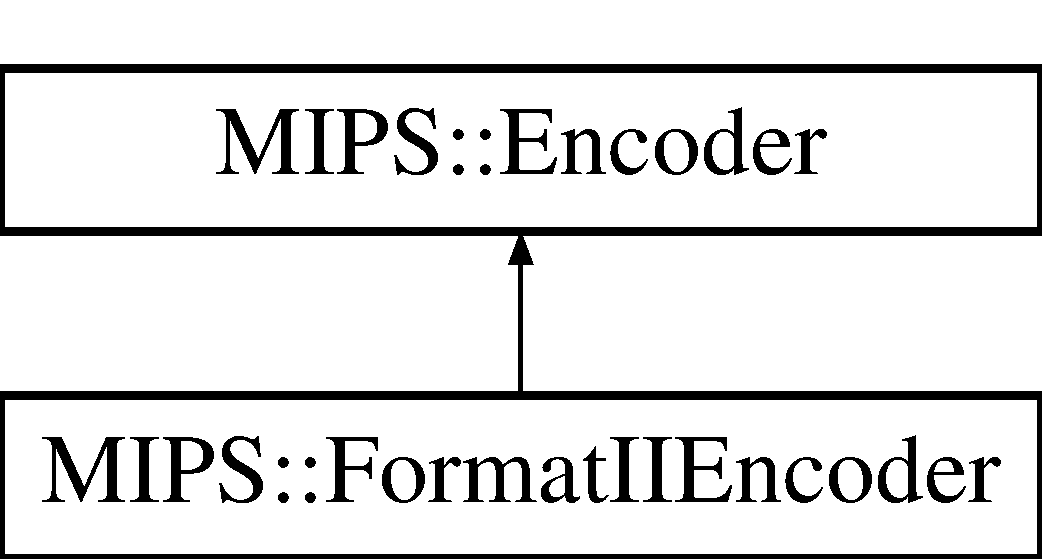
\includegraphics[height=2.000000cm]{classMIPS_1_1FormatIIEncoder}
\end{center}
\end{figure}
\subsection*{Public Member Functions}
\begin{DoxyCompactItemize}
\item 
\hyperlink{core_8hpp_aa514fd240a0e29abb2a2e4c805d7f1a4}{instruction\+\_\+t} \hyperlink{classMIPS_1_1FormatIIEncoder_aaf5f5f9d4c9b6b63b150b239cb5b03fe}{encode} ()
\item 
void \hyperlink{classMIPS_1_1FormatIIEncoder_aa988c9638985b07eea58f3e11ff4c2e7}{parse} (std\+::vector$<$ char $\ast$ $>$ \&params)
\end{DoxyCompactItemize}
\subsection*{Additional Inherited Members}


\subsection{Detailed Description}
Codificador responsável por transformar uma instrução assembly em uma instrução binária, seguindo o formato de instrução no formato II.

\begin{DoxyAuthor}{Author}
Matheus Nogueira 
\end{DoxyAuthor}


\subsection{Member Function Documentation}
\index{M\+I\+P\+S\+::\+Format\+I\+I\+Encoder@{M\+I\+P\+S\+::\+Format\+I\+I\+Encoder}!encode@{encode}}
\index{encode@{encode}!M\+I\+P\+S\+::\+Format\+I\+I\+Encoder@{M\+I\+P\+S\+::\+Format\+I\+I\+Encoder}}
\subsubsection[{\texorpdfstring{encode()}{encode()}}]{\setlength{\rightskip}{0pt plus 5cm}{\bf instruction\+\_\+t} M\+I\+P\+S\+::\+Format\+I\+I\+Encoder\+::encode (
\begin{DoxyParamCaption}
{}
\end{DoxyParamCaption}
)\hspace{0.3cm}{\ttfamily [virtual]}}\hypertarget{classMIPS_1_1FormatIIEncoder_aaf5f5f9d4c9b6b63b150b239cb5b03fe}{}\label{classMIPS_1_1FormatIIEncoder_aaf5f5f9d4c9b6b63b150b239cb5b03fe}
Codifica uma instrução assembly do formato II para uma instrução binária.

\begin{DoxyReturn}{Returns}
instrução binária de 16 bits 
\end{DoxyReturn}


Implements \hyperlink{classMIPS_1_1Encoder_ac3ea6ce91eabd41b3c512a39ee4c3550}{M\+I\+P\+S\+::\+Encoder}.

\index{M\+I\+P\+S\+::\+Format\+I\+I\+Encoder@{M\+I\+P\+S\+::\+Format\+I\+I\+Encoder}!parse@{parse}}
\index{parse@{parse}!M\+I\+P\+S\+::\+Format\+I\+I\+Encoder@{M\+I\+P\+S\+::\+Format\+I\+I\+Encoder}}
\subsubsection[{\texorpdfstring{parse(std\+::vector$<$ char $\ast$ $>$ \&params)}{parse(std::vector< char * > &params)}}]{\setlength{\rightskip}{0pt plus 5cm}void M\+I\+P\+S\+::\+Format\+I\+I\+Encoder\+::parse (
\begin{DoxyParamCaption}
\item[{std\+::vector$<$ char $\ast$ $>$ \&}]{params}
\end{DoxyParamCaption}
)\hspace{0.3cm}{\ttfamily [virtual]}}\hypertarget{classMIPS_1_1FormatIIEncoder_aa988c9638985b07eea58f3e11ff4c2e7}{}\label{classMIPS_1_1FormatIIEncoder_aa988c9638985b07eea58f3e11ff4c2e7}
Realiza uma varredura na instrução assembly e define seus campos binários.


\begin{DoxyParams}{Parameters}
{\em params} & vector de parâmetros da instrução \\
\hline
\end{DoxyParams}


Implements \hyperlink{classMIPS_1_1Encoder_a4a29c42d601460be8e8d353d8fc0da34}{M\+I\+P\+S\+::\+Encoder}.



The documentation for this class was generated from the following file\+:\begin{DoxyCompactItemize}
\item 
include/mips/interpreter/encoder/\hyperlink{format__II__encoder_8hpp}{format\+\_\+\+I\+I\+\_\+encoder.\+hpp}\end{DoxyCompactItemize}

\hypertarget{classMIPS_1_1FormatIIIEncoder}{}\section{M\+I\+PS\+:\+:Format\+I\+I\+I\+Encoder Class Reference}
\label{classMIPS_1_1FormatIIIEncoder}\index{M\+I\+P\+S\+::\+Format\+I\+I\+I\+Encoder@{M\+I\+P\+S\+::\+Format\+I\+I\+I\+Encoder}}


{\ttfamily \#include $<$format\+\_\+\+I\+I\+I\+\_\+encoder.\+hpp$>$}

Inheritance diagram for M\+I\+PS\+:\+:Format\+I\+I\+I\+Encoder\+:\begin{figure}[H]
\begin{center}
\leavevmode
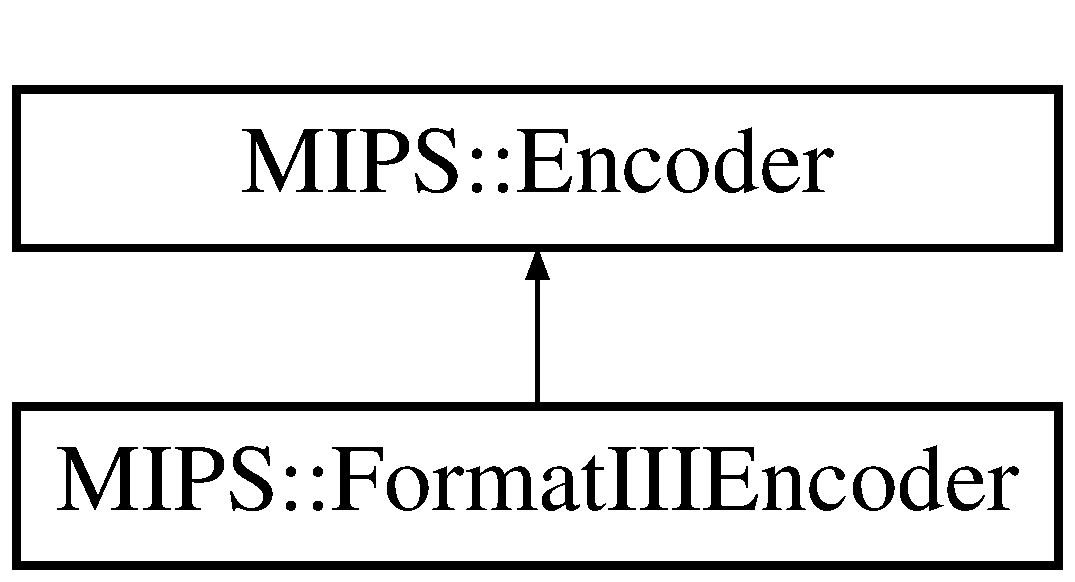
\includegraphics[height=2.000000cm]{classMIPS_1_1FormatIIIEncoder}
\end{center}
\end{figure}
\subsection*{Public Member Functions}
\begin{DoxyCompactItemize}
\item 
\hyperlink{core_8hpp_aa514fd240a0e29abb2a2e4c805d7f1a4}{instruction\+\_\+t} \hyperlink{classMIPS_1_1FormatIIIEncoder_ab243fc73a602716a7ed15f13dbd2b695}{encode} ()
\item 
void \hyperlink{classMIPS_1_1FormatIIIEncoder_a06c8d98fe19c20d5e4f0986d7d500637}{parse} (std\+::vector$<$ char $\ast$ $>$ \&params)
\end{DoxyCompactItemize}
\subsection*{Additional Inherited Members}


\subsection{Detailed Description}
Codificador responsável por transformar uma instrução assembly em uma instrução binária, seguindo o formato de instrução no formato I\+II.

\begin{DoxyAuthor}{Author}
Matheus Nogueira 
\end{DoxyAuthor}


\subsection{Member Function Documentation}
\index{M\+I\+P\+S\+::\+Format\+I\+I\+I\+Encoder@{M\+I\+P\+S\+::\+Format\+I\+I\+I\+Encoder}!encode@{encode}}
\index{encode@{encode}!M\+I\+P\+S\+::\+Format\+I\+I\+I\+Encoder@{M\+I\+P\+S\+::\+Format\+I\+I\+I\+Encoder}}
\subsubsection[{\texorpdfstring{encode()}{encode()}}]{\setlength{\rightskip}{0pt plus 5cm}{\bf instruction\+\_\+t} M\+I\+P\+S\+::\+Format\+I\+I\+I\+Encoder\+::encode (
\begin{DoxyParamCaption}
{}
\end{DoxyParamCaption}
)\hspace{0.3cm}{\ttfamily [virtual]}}\hypertarget{classMIPS_1_1FormatIIIEncoder_ab243fc73a602716a7ed15f13dbd2b695}{}\label{classMIPS_1_1FormatIIIEncoder_ab243fc73a602716a7ed15f13dbd2b695}
Codifica uma instrução assembly do formato I\+II para uma instrução binária.

\begin{DoxyReturn}{Returns}
instrução binária de 16 bits 
\end{DoxyReturn}


Implements \hyperlink{classMIPS_1_1Encoder_ac3ea6ce91eabd41b3c512a39ee4c3550}{M\+I\+P\+S\+::\+Encoder}.

\index{M\+I\+P\+S\+::\+Format\+I\+I\+I\+Encoder@{M\+I\+P\+S\+::\+Format\+I\+I\+I\+Encoder}!parse@{parse}}
\index{parse@{parse}!M\+I\+P\+S\+::\+Format\+I\+I\+I\+Encoder@{M\+I\+P\+S\+::\+Format\+I\+I\+I\+Encoder}}
\subsubsection[{\texorpdfstring{parse(std\+::vector$<$ char $\ast$ $>$ \&params)}{parse(std::vector< char * > &params)}}]{\setlength{\rightskip}{0pt plus 5cm}void M\+I\+P\+S\+::\+Format\+I\+I\+I\+Encoder\+::parse (
\begin{DoxyParamCaption}
\item[{std\+::vector$<$ char $\ast$ $>$ \&}]{params}
\end{DoxyParamCaption}
)\hspace{0.3cm}{\ttfamily [virtual]}}\hypertarget{classMIPS_1_1FormatIIIEncoder_a06c8d98fe19c20d5e4f0986d7d500637}{}\label{classMIPS_1_1FormatIIIEncoder_a06c8d98fe19c20d5e4f0986d7d500637}
Realiza uma varredura na instrução assembly e define seus campos binários.


\begin{DoxyParams}{Parameters}
{\em params} & vector de parâmetros da instrução \\
\hline
\end{DoxyParams}


Implements \hyperlink{classMIPS_1_1Encoder_a4a29c42d601460be8e8d353d8fc0da34}{M\+I\+P\+S\+::\+Encoder}.



The documentation for this class was generated from the following file\+:\begin{DoxyCompactItemize}
\item 
include/mips/interpreter/encoder/\hyperlink{format__III__encoder_8hpp}{format\+\_\+\+I\+I\+I\+\_\+encoder.\+hpp}\end{DoxyCompactItemize}

\hypertarget{classMIPS_1_1FormatIVEncoder}{}\section{M\+I\+PS\+:\+:Format\+I\+V\+Encoder Class Reference}
\label{classMIPS_1_1FormatIVEncoder}\index{M\+I\+P\+S\+::\+Format\+I\+V\+Encoder@{M\+I\+P\+S\+::\+Format\+I\+V\+Encoder}}


{\ttfamily \#include $<$format\+\_\+\+I\+V\+\_\+encoder.\+hpp$>$}

Inheritance diagram for M\+I\+PS\+:\+:Format\+I\+V\+Encoder\+:\begin{figure}[H]
\begin{center}
\leavevmode
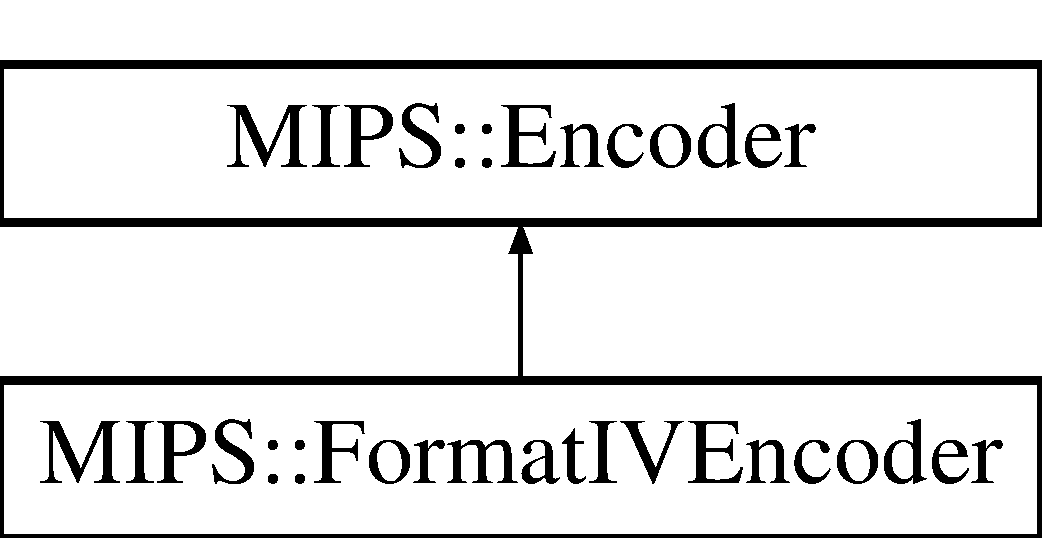
\includegraphics[height=2.000000cm]{classMIPS_1_1FormatIVEncoder}
\end{center}
\end{figure}
\subsection*{Public Member Functions}
\begin{DoxyCompactItemize}
\item 
\hyperlink{core_8hpp_aa514fd240a0e29abb2a2e4c805d7f1a4}{instruction\+\_\+t} \hyperlink{classMIPS_1_1FormatIVEncoder_a1d23ca4c9c81536dd43a18dc8dd43f97}{encode} ()
\item 
void \hyperlink{classMIPS_1_1FormatIVEncoder_a42f251011a97af63a707b4d0607e18a9}{parse} (std\+::vector$<$ char $\ast$ $>$ \&params)
\end{DoxyCompactItemize}
\subsection*{Additional Inherited Members}


\subsection{Detailed Description}
Codificador responsável por transformar uma instrução assembly em uma instrução binária, seguindo o formato de instrução no formato IV.

\begin{DoxyAuthor}{Author}
Matheus Nogueira 
\end{DoxyAuthor}


\subsection{Member Function Documentation}
\index{M\+I\+P\+S\+::\+Format\+I\+V\+Encoder@{M\+I\+P\+S\+::\+Format\+I\+V\+Encoder}!encode@{encode}}
\index{encode@{encode}!M\+I\+P\+S\+::\+Format\+I\+V\+Encoder@{M\+I\+P\+S\+::\+Format\+I\+V\+Encoder}}
\subsubsection[{\texorpdfstring{encode()}{encode()}}]{\setlength{\rightskip}{0pt plus 5cm}{\bf instruction\+\_\+t} M\+I\+P\+S\+::\+Format\+I\+V\+Encoder\+::encode (
\begin{DoxyParamCaption}
{}
\end{DoxyParamCaption}
)\hspace{0.3cm}{\ttfamily [virtual]}}\hypertarget{classMIPS_1_1FormatIVEncoder_a1d23ca4c9c81536dd43a18dc8dd43f97}{}\label{classMIPS_1_1FormatIVEncoder_a1d23ca4c9c81536dd43a18dc8dd43f97}
Codifica uma instrução assembly do formato IV para uma instrução binária.

\begin{DoxyReturn}{Returns}
instrução binária de 16 bits 
\end{DoxyReturn}


Implements \hyperlink{classMIPS_1_1Encoder_ac3ea6ce91eabd41b3c512a39ee4c3550}{M\+I\+P\+S\+::\+Encoder}.

\index{M\+I\+P\+S\+::\+Format\+I\+V\+Encoder@{M\+I\+P\+S\+::\+Format\+I\+V\+Encoder}!parse@{parse}}
\index{parse@{parse}!M\+I\+P\+S\+::\+Format\+I\+V\+Encoder@{M\+I\+P\+S\+::\+Format\+I\+V\+Encoder}}
\subsubsection[{\texorpdfstring{parse(std\+::vector$<$ char $\ast$ $>$ \&params)}{parse(std::vector< char * > &params)}}]{\setlength{\rightskip}{0pt plus 5cm}void M\+I\+P\+S\+::\+Format\+I\+V\+Encoder\+::parse (
\begin{DoxyParamCaption}
\item[{std\+::vector$<$ char $\ast$ $>$ \&}]{params}
\end{DoxyParamCaption}
)\hspace{0.3cm}{\ttfamily [virtual]}}\hypertarget{classMIPS_1_1FormatIVEncoder_a42f251011a97af63a707b4d0607e18a9}{}\label{classMIPS_1_1FormatIVEncoder_a42f251011a97af63a707b4d0607e18a9}
Realiza uma varredura na instrução assembly e define seus campos binários.


\begin{DoxyParams}{Parameters}
{\em params} & vector de parâmetros da instrução \\
\hline
\end{DoxyParams}


Implements \hyperlink{classMIPS_1_1Encoder_a4a29c42d601460be8e8d353d8fc0da34}{M\+I\+P\+S\+::\+Encoder}.



The documentation for this class was generated from the following file\+:\begin{DoxyCompactItemize}
\item 
include/mips/interpreter/encoder/\hyperlink{format__IV__encoder_8hpp}{format\+\_\+\+I\+V\+\_\+encoder.\+hpp}\end{DoxyCompactItemize}

\hypertarget{classMIPS_1_1FormatVEncoder}{}\section{M\+I\+PS\+:\+:Format\+V\+Encoder Class Reference}
\label{classMIPS_1_1FormatVEncoder}\index{M\+I\+P\+S\+::\+Format\+V\+Encoder@{M\+I\+P\+S\+::\+Format\+V\+Encoder}}


{\ttfamily \#include $<$format\+\_\+\+V\+\_\+encoder.\+hpp$>$}

Inheritance diagram for M\+I\+PS\+:\+:Format\+V\+Encoder\+:\begin{figure}[H]
\begin{center}
\leavevmode
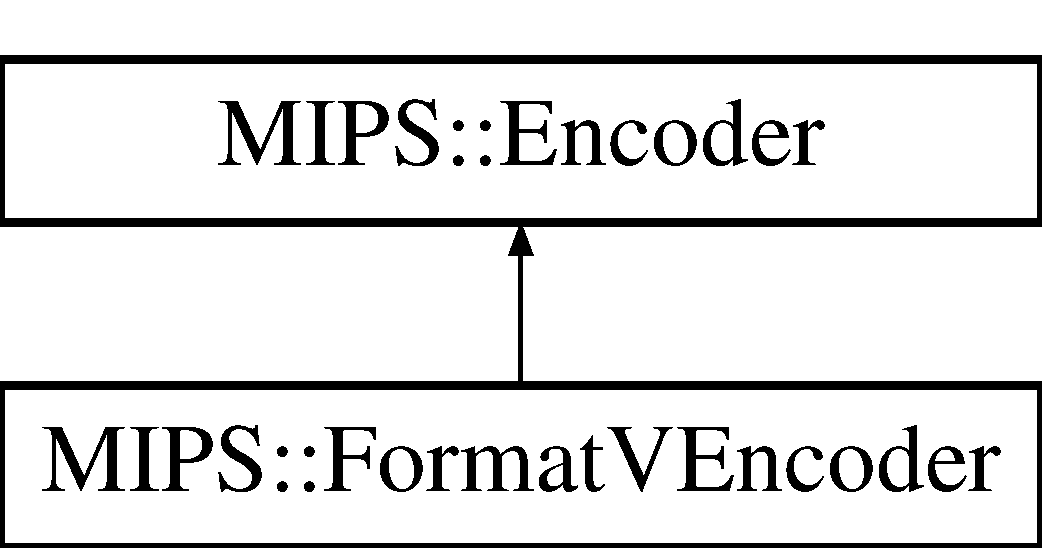
\includegraphics[height=2.000000cm]{classMIPS_1_1FormatVEncoder}
\end{center}
\end{figure}
\subsection*{Public Member Functions}
\begin{DoxyCompactItemize}
\item 
\hyperlink{core_8hpp_aa514fd240a0e29abb2a2e4c805d7f1a4}{instruction\+\_\+t} \hyperlink{classMIPS_1_1FormatVEncoder_a95e96820cef484d427c64145006d8837}{encode} ()
\item 
void \hyperlink{classMIPS_1_1FormatVEncoder_af73c15fbc94eac0f8b28e6d7fa2e4dc2}{parse} (std\+::vector$<$ char $\ast$ $>$ \&params)
\end{DoxyCompactItemize}
\subsection*{Additional Inherited Members}


\subsection{Detailed Description}
Codificador responsável por transformar uma instrução assembly em uma instrução binária, seguindo o formato de instrução no formato V.

\begin{DoxyAuthor}{Author}
Matheus Nogueira 
\end{DoxyAuthor}


\subsection{Member Function Documentation}
\index{M\+I\+P\+S\+::\+Format\+V\+Encoder@{M\+I\+P\+S\+::\+Format\+V\+Encoder}!encode@{encode}}
\index{encode@{encode}!M\+I\+P\+S\+::\+Format\+V\+Encoder@{M\+I\+P\+S\+::\+Format\+V\+Encoder}}
\subsubsection[{\texorpdfstring{encode()}{encode()}}]{\setlength{\rightskip}{0pt plus 5cm}{\bf instruction\+\_\+t} M\+I\+P\+S\+::\+Format\+V\+Encoder\+::encode (
\begin{DoxyParamCaption}
{}
\end{DoxyParamCaption}
)\hspace{0.3cm}{\ttfamily [virtual]}}\hypertarget{classMIPS_1_1FormatVEncoder_a95e96820cef484d427c64145006d8837}{}\label{classMIPS_1_1FormatVEncoder_a95e96820cef484d427c64145006d8837}
Codifica uma instrução assembly do formato V para uma instrução binária.

\begin{DoxyReturn}{Returns}
instrução binária de 16 bits 
\end{DoxyReturn}


Implements \hyperlink{classMIPS_1_1Encoder_ac3ea6ce91eabd41b3c512a39ee4c3550}{M\+I\+P\+S\+::\+Encoder}.

\index{M\+I\+P\+S\+::\+Format\+V\+Encoder@{M\+I\+P\+S\+::\+Format\+V\+Encoder}!parse@{parse}}
\index{parse@{parse}!M\+I\+P\+S\+::\+Format\+V\+Encoder@{M\+I\+P\+S\+::\+Format\+V\+Encoder}}
\subsubsection[{\texorpdfstring{parse(std\+::vector$<$ char $\ast$ $>$ \&params)}{parse(std::vector< char * > &params)}}]{\setlength{\rightskip}{0pt plus 5cm}void M\+I\+P\+S\+::\+Format\+V\+Encoder\+::parse (
\begin{DoxyParamCaption}
\item[{std\+::vector$<$ char $\ast$ $>$ \&}]{params}
\end{DoxyParamCaption}
)\hspace{0.3cm}{\ttfamily [virtual]}}\hypertarget{classMIPS_1_1FormatVEncoder_af73c15fbc94eac0f8b28e6d7fa2e4dc2}{}\label{classMIPS_1_1FormatVEncoder_af73c15fbc94eac0f8b28e6d7fa2e4dc2}
Realiza uma varredura na instrução assembly e define seus campos binários.


\begin{DoxyParams}{Parameters}
{\em params} & vector de parâmetros da instrução \\
\hline
\end{DoxyParams}


Implements \hyperlink{classMIPS_1_1Encoder_a4a29c42d601460be8e8d353d8fc0da34}{M\+I\+P\+S\+::\+Encoder}.



The documentation for this class was generated from the following file\+:\begin{DoxyCompactItemize}
\item 
include/mips/interpreter/encoder/\hyperlink{format__V__encoder_8hpp}{format\+\_\+\+V\+\_\+encoder.\+hpp}\end{DoxyCompactItemize}

\hypertarget{classMIPS_1_1FormatVIEncoder}{}\section{M\+I\+PS\+:\+:Format\+V\+I\+Encoder Class Reference}
\label{classMIPS_1_1FormatVIEncoder}\index{M\+I\+P\+S\+::\+Format\+V\+I\+Encoder@{M\+I\+P\+S\+::\+Format\+V\+I\+Encoder}}


{\ttfamily \#include $<$format\+\_\+\+V\+I\+\_\+encoder.\+hpp$>$}

Inheritance diagram for M\+I\+PS\+:\+:Format\+V\+I\+Encoder\+:\begin{figure}[H]
\begin{center}
\leavevmode
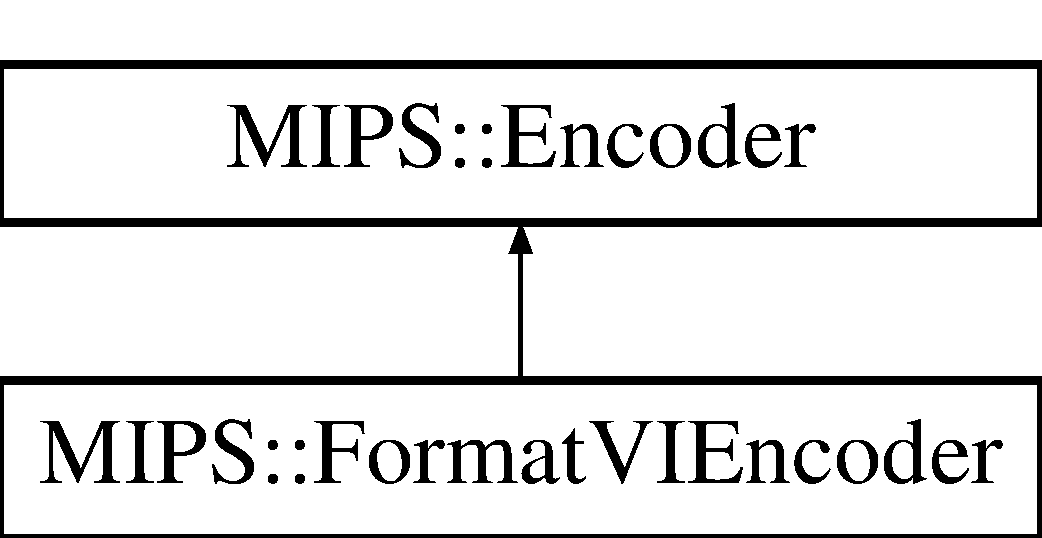
\includegraphics[height=2.000000cm]{classMIPS_1_1FormatVIEncoder}
\end{center}
\end{figure}
\subsection*{Public Member Functions}
\begin{DoxyCompactItemize}
\item 
\hyperlink{core_8hpp_aa514fd240a0e29abb2a2e4c805d7f1a4}{instruction\+\_\+t} \hyperlink{classMIPS_1_1FormatVIEncoder_ae0a892a24d712d260f80dbc6e85b7090}{encode} ()
\item 
void \hyperlink{classMIPS_1_1FormatVIEncoder_a4cec696ab9deca5b957ddbab97139631}{parse} (std\+::vector$<$ char $\ast$ $>$ \&params)
\end{DoxyCompactItemize}
\subsection*{Additional Inherited Members}


\subsection{Detailed Description}
Codificador responsável por transformar uma instrução assembly em uma instrução binária, seguindo o formato de instrução no formato VI.

\begin{DoxyAuthor}{Author}
Matheus Nogueira 
\end{DoxyAuthor}


\subsection{Member Function Documentation}
\index{M\+I\+P\+S\+::\+Format\+V\+I\+Encoder@{M\+I\+P\+S\+::\+Format\+V\+I\+Encoder}!encode@{encode}}
\index{encode@{encode}!M\+I\+P\+S\+::\+Format\+V\+I\+Encoder@{M\+I\+P\+S\+::\+Format\+V\+I\+Encoder}}
\subsubsection[{\texorpdfstring{encode()}{encode()}}]{\setlength{\rightskip}{0pt plus 5cm}{\bf instruction\+\_\+t} M\+I\+P\+S\+::\+Format\+V\+I\+Encoder\+::encode (
\begin{DoxyParamCaption}
{}
\end{DoxyParamCaption}
)\hspace{0.3cm}{\ttfamily [virtual]}}\hypertarget{classMIPS_1_1FormatVIEncoder_ae0a892a24d712d260f80dbc6e85b7090}{}\label{classMIPS_1_1FormatVIEncoder_ae0a892a24d712d260f80dbc6e85b7090}
Codifica uma instrução assembly do formato V para uma instrução binária.

\begin{DoxyReturn}{Returns}
instrução binária de 16 bits 
\end{DoxyReturn}


Implements \hyperlink{classMIPS_1_1Encoder_ac3ea6ce91eabd41b3c512a39ee4c3550}{M\+I\+P\+S\+::\+Encoder}.

\index{M\+I\+P\+S\+::\+Format\+V\+I\+Encoder@{M\+I\+P\+S\+::\+Format\+V\+I\+Encoder}!parse@{parse}}
\index{parse@{parse}!M\+I\+P\+S\+::\+Format\+V\+I\+Encoder@{M\+I\+P\+S\+::\+Format\+V\+I\+Encoder}}
\subsubsection[{\texorpdfstring{parse(std\+::vector$<$ char $\ast$ $>$ \&params)}{parse(std::vector< char * > &params)}}]{\setlength{\rightskip}{0pt plus 5cm}void M\+I\+P\+S\+::\+Format\+V\+I\+Encoder\+::parse (
\begin{DoxyParamCaption}
\item[{std\+::vector$<$ char $\ast$ $>$ \&}]{params}
\end{DoxyParamCaption}
)\hspace{0.3cm}{\ttfamily [virtual]}}\hypertarget{classMIPS_1_1FormatVIEncoder_a4cec696ab9deca5b957ddbab97139631}{}\label{classMIPS_1_1FormatVIEncoder_a4cec696ab9deca5b957ddbab97139631}
Realiza uma varredura na instrução assembly e define seus campos binários.


\begin{DoxyParams}{Parameters}
{\em params} & vector de parâmetros da instrução \\
\hline
\end{DoxyParams}


Implements \hyperlink{classMIPS_1_1Encoder_a4a29c42d601460be8e8d353d8fc0da34}{M\+I\+P\+S\+::\+Encoder}.



The documentation for this class was generated from the following file\+:\begin{DoxyCompactItemize}
\item 
include/mips/interpreter/encoder/\hyperlink{format__VI__encoder_8hpp}{format\+\_\+\+V\+I\+\_\+encoder.\+hpp}\end{DoxyCompactItemize}

\hypertarget{classMIPS_1_1FormatVIIEncoder}{}\section{M\+I\+PS\+:\+:Format\+V\+I\+I\+Encoder Class Reference}
\label{classMIPS_1_1FormatVIIEncoder}\index{M\+I\+P\+S\+::\+Format\+V\+I\+I\+Encoder@{M\+I\+P\+S\+::\+Format\+V\+I\+I\+Encoder}}


{\ttfamily \#include $<$format\+\_\+\+V\+I\+I\+\_\+encoder.\+hpp$>$}

Inheritance diagram for M\+I\+PS\+:\+:Format\+V\+I\+I\+Encoder\+:\begin{figure}[H]
\begin{center}
\leavevmode
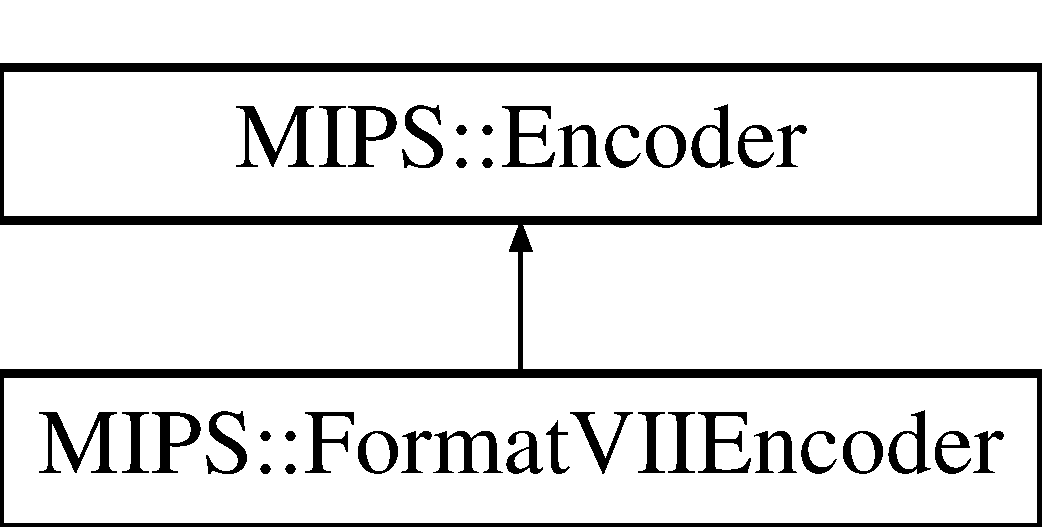
\includegraphics[height=2.000000cm]{classMIPS_1_1FormatVIIEncoder}
\end{center}
\end{figure}
\subsection*{Public Member Functions}
\begin{DoxyCompactItemize}
\item 
\hyperlink{core_8hpp_aa514fd240a0e29abb2a2e4c805d7f1a4}{instruction\+\_\+t} \hyperlink{classMIPS_1_1FormatVIIEncoder_a2afcc51d8983491e39d145766639b995}{encode} ()
\item 
void \hyperlink{classMIPS_1_1FormatVIIEncoder_a67272c7aad39c6f49c4aa162119215ba}{parse} (std\+::vector$<$ char $\ast$ $>$ \&params)
\end{DoxyCompactItemize}
\subsection*{Additional Inherited Members}


\subsection{Detailed Description}
Codificador responsável por transformar uma instrução assembly em uma instrução binária, seguindo o formato de instrução no formato V\+II.

\begin{DoxyAuthor}{Author}
Matheus Nogueira 
\end{DoxyAuthor}


\subsection{Member Function Documentation}
\index{M\+I\+P\+S\+::\+Format\+V\+I\+I\+Encoder@{M\+I\+P\+S\+::\+Format\+V\+I\+I\+Encoder}!encode@{encode}}
\index{encode@{encode}!M\+I\+P\+S\+::\+Format\+V\+I\+I\+Encoder@{M\+I\+P\+S\+::\+Format\+V\+I\+I\+Encoder}}
\subsubsection[{\texorpdfstring{encode()}{encode()}}]{\setlength{\rightskip}{0pt plus 5cm}{\bf instruction\+\_\+t} M\+I\+P\+S\+::\+Format\+V\+I\+I\+Encoder\+::encode (
\begin{DoxyParamCaption}
{}
\end{DoxyParamCaption}
)\hspace{0.3cm}{\ttfamily [virtual]}}\hypertarget{classMIPS_1_1FormatVIIEncoder_a2afcc51d8983491e39d145766639b995}{}\label{classMIPS_1_1FormatVIIEncoder_a2afcc51d8983491e39d145766639b995}
Codifica uma instrução assembly do formato V para uma instrução binária.

\begin{DoxyReturn}{Returns}
instrução binária de 16 bits 
\end{DoxyReturn}


Implements \hyperlink{classMIPS_1_1Encoder_ac3ea6ce91eabd41b3c512a39ee4c3550}{M\+I\+P\+S\+::\+Encoder}.

\index{M\+I\+P\+S\+::\+Format\+V\+I\+I\+Encoder@{M\+I\+P\+S\+::\+Format\+V\+I\+I\+Encoder}!parse@{parse}}
\index{parse@{parse}!M\+I\+P\+S\+::\+Format\+V\+I\+I\+Encoder@{M\+I\+P\+S\+::\+Format\+V\+I\+I\+Encoder}}
\subsubsection[{\texorpdfstring{parse(std\+::vector$<$ char $\ast$ $>$ \&params)}{parse(std::vector< char * > &params)}}]{\setlength{\rightskip}{0pt plus 5cm}void M\+I\+P\+S\+::\+Format\+V\+I\+I\+Encoder\+::parse (
\begin{DoxyParamCaption}
\item[{std\+::vector$<$ char $\ast$ $>$ \&}]{params}
\end{DoxyParamCaption}
)\hspace{0.3cm}{\ttfamily [virtual]}}\hypertarget{classMIPS_1_1FormatVIIEncoder_a67272c7aad39c6f49c4aa162119215ba}{}\label{classMIPS_1_1FormatVIIEncoder_a67272c7aad39c6f49c4aa162119215ba}
Realiza uma varredura na instrução assembly e define seus campos binários.


\begin{DoxyParams}{Parameters}
{\em params} & vector de parâmetros da instrução \\
\hline
\end{DoxyParams}


Implements \hyperlink{classMIPS_1_1Encoder_a4a29c42d601460be8e8d353d8fc0da34}{M\+I\+P\+S\+::\+Encoder}.



The documentation for this class was generated from the following file\+:\begin{DoxyCompactItemize}
\item 
include/mips/interpreter/encoder/\hyperlink{format__VII__encoder_8hpp}{format\+\_\+\+V\+I\+I\+\_\+encoder.\+hpp}\end{DoxyCompactItemize}

\hypertarget{classMIPS_1_1FullAdder}{}\section{M\+I\+PS\+:\+:Full\+Adder Class Reference}
\label{classMIPS_1_1FullAdder}\index{M\+I\+P\+S\+::\+Full\+Adder@{M\+I\+P\+S\+::\+Full\+Adder}}


{\ttfamily \#include $<$full\+\_\+adder.\+hpp$>$}

\subsection*{Public Member Functions}
\begin{DoxyCompactItemize}
\item 
\hyperlink{classMIPS_1_1FullAdder_a6b2eecd1b2720d87322810a72ab0cf16}{Full\+Adder} ()
\item 
\hyperlink{core_8hpp_adc265a970bc35995b5879784bbb3f1b7}{bit16\+\_\+t} \hyperlink{classMIPS_1_1FullAdder_a19fda5cf604f2b04f55ebe8aa3972c7f}{add} (\hyperlink{core_8hpp_adc265a970bc35995b5879784bbb3f1b7}{bit16\+\_\+t} a, \hyperlink{core_8hpp_adc265a970bc35995b5879784bbb3f1b7}{bit16\+\_\+t} b, \hyperlink{core_8hpp_a6074bae122ae7b527864eec42c728c3c}{bit8\+\_\+t} c=0)
\item 
bool \hyperlink{classMIPS_1_1FullAdder_ad700abfd3da45fe8d25a9f1b071378a8}{overflow} ()
\end{DoxyCompactItemize}


\subsection{Detailed Description}
Classe responsável por realizar as operações de um somador de 16 bits.

\begin{DoxyAuthor}{Author}
Matheus Nogueira 
\end{DoxyAuthor}


\subsection{Constructor \& Destructor Documentation}
\index{M\+I\+P\+S\+::\+Full\+Adder@{M\+I\+P\+S\+::\+Full\+Adder}!Full\+Adder@{Full\+Adder}}
\index{Full\+Adder@{Full\+Adder}!M\+I\+P\+S\+::\+Full\+Adder@{M\+I\+P\+S\+::\+Full\+Adder}}
\subsubsection[{\texorpdfstring{Full\+Adder()}{FullAdder()}}]{\setlength{\rightskip}{0pt plus 5cm}M\+I\+P\+S\+::\+Full\+Adder\+::\+Full\+Adder (
\begin{DoxyParamCaption}
{}
\end{DoxyParamCaption}
)}\hypertarget{classMIPS_1_1FullAdder_a6b2eecd1b2720d87322810a72ab0cf16}{}\label{classMIPS_1_1FullAdder_a6b2eecd1b2720d87322810a72ab0cf16}
Cria um novo somador. 

\subsection{Member Function Documentation}
\index{M\+I\+P\+S\+::\+Full\+Adder@{M\+I\+P\+S\+::\+Full\+Adder}!add@{add}}
\index{add@{add}!M\+I\+P\+S\+::\+Full\+Adder@{M\+I\+P\+S\+::\+Full\+Adder}}
\subsubsection[{\texorpdfstring{add(bit16\+\_\+t a, bit16\+\_\+t b, bit8\+\_\+t c=0)}{add(bit16_t a, bit16_t b, bit8_t c=0)}}]{\setlength{\rightskip}{0pt plus 5cm}{\bf bit16\+\_\+t} M\+I\+P\+S\+::\+Full\+Adder\+::add (
\begin{DoxyParamCaption}
\item[{{\bf bit16\+\_\+t}}]{a, }
\item[{{\bf bit16\+\_\+t}}]{b, }
\item[{{\bf bit8\+\_\+t}}]{c = {\ttfamily 0}}
\end{DoxyParamCaption}
)}\hypertarget{classMIPS_1_1FullAdder_a19fda5cf604f2b04f55ebe8aa3972c7f}{}\label{classMIPS_1_1FullAdder_a19fda5cf604f2b04f55ebe8aa3972c7f}
Soma dois números de 16 bits.


\begin{DoxyParams}{Parameters}
{\em a} & primeiro parametro da soma \\
\hline
{\em b} & segundo parametro da soma \\
\hline
{\em c} & carry de entrada (padrão\+: 0) \\
\hline
\end{DoxyParams}
\begin{DoxyReturn}{Returns}
resultado da soma entre a e b 
\end{DoxyReturn}
\index{M\+I\+P\+S\+::\+Full\+Adder@{M\+I\+P\+S\+::\+Full\+Adder}!overflow@{overflow}}
\index{overflow@{overflow}!M\+I\+P\+S\+::\+Full\+Adder@{M\+I\+P\+S\+::\+Full\+Adder}}
\subsubsection[{\texorpdfstring{overflow()}{overflow()}}]{\setlength{\rightskip}{0pt plus 5cm}bool M\+I\+P\+S\+::\+Full\+Adder\+::overflow (
\begin{DoxyParamCaption}
{}
\end{DoxyParamCaption}
)}\hypertarget{classMIPS_1_1FullAdder_ad700abfd3da45fe8d25a9f1b071378a8}{}\label{classMIPS_1_1FullAdder_ad700abfd3da45fe8d25a9f1b071378a8}
Verifica se houve overflow na operação de adição.

\begin{DoxyReturn}{Returns}
true se houve overflow. 
\end{DoxyReturn}


The documentation for this class was generated from the following file\+:\begin{DoxyCompactItemize}
\item 
include/mips/circuits/\hyperlink{full__adder_8hpp}{full\+\_\+adder.\+hpp}\end{DoxyCompactItemize}

\hypertarget{classMIPS_1_1IncaInstruction}{}\section{M\+I\+PS\+:\+:Inca\+Instruction Class Reference}
\label{classMIPS_1_1IncaInstruction}\index{M\+I\+P\+S\+::\+Inca\+Instruction@{M\+I\+P\+S\+::\+Inca\+Instruction}}


{\ttfamily \#include $<$inca.\+hpp$>$}

Inheritance diagram for M\+I\+PS\+:\+:Inca\+Instruction\+:\begin{figure}[H]
\begin{center}
\leavevmode
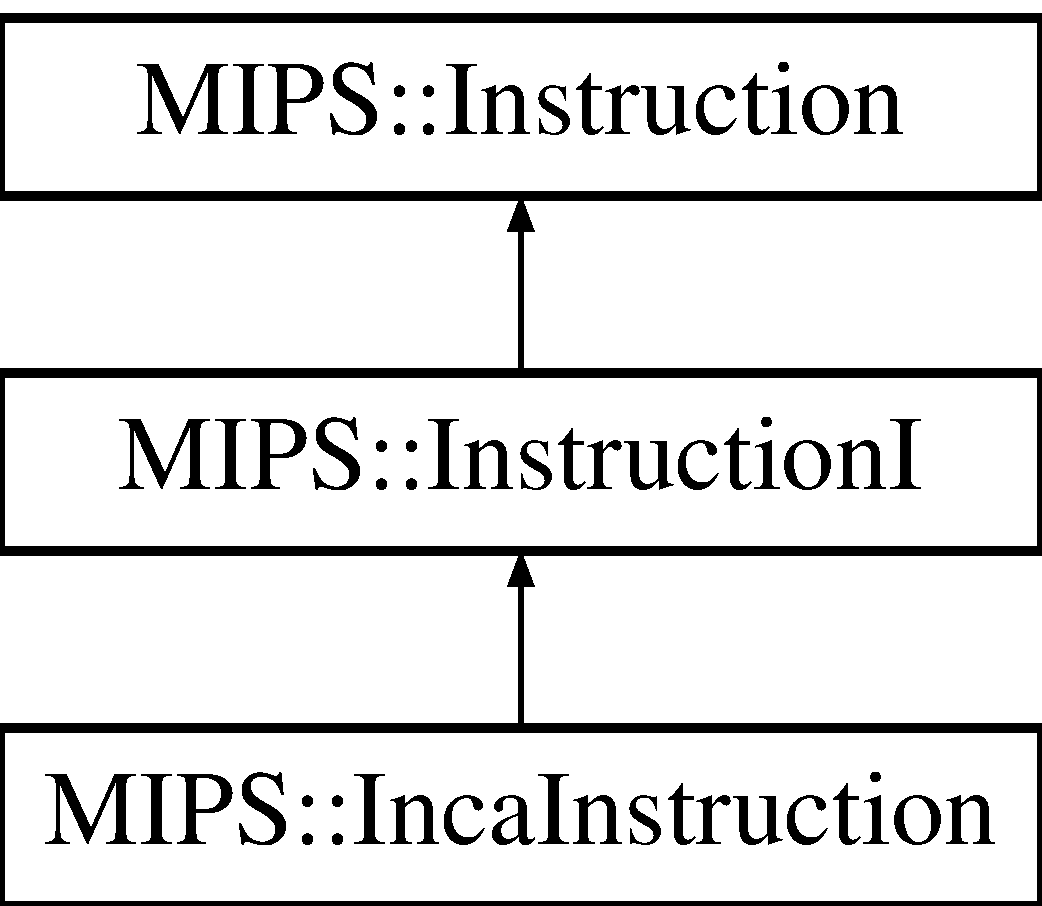
\includegraphics[height=3.000000cm]{classMIPS_1_1IncaInstruction}
\end{center}
\end{figure}
\subsection*{Public Member Functions}
\begin{DoxyCompactItemize}
\item 
\hyperlink{classMIPS_1_1IncaInstruction_a03f08716ad682f74db7aef71961c4b09}{Inca\+Instruction} (\hyperlink{core_8hpp_a6074bae122ae7b527864eec42c728c3c}{bit8\+\_\+t} \hyperlink{classMIPS_1_1Instruction_a45cc6808b5dde8a5d41067d148b55476}{opcode}, \hyperlink{classMIPS_1_1Register}{Register} $\ast$\hyperlink{classMIPS_1_1InstructionI_a2be191d5b3dce505e2e626ec02eb4d62}{rs}, \hyperlink{classMIPS_1_1Register}{Register} $\ast$\hyperlink{classMIPS_1_1InstructionI_add1db07a5c954f35271de8c8a5737487}{rt}, \hyperlink{core_8hpp_a6074bae122ae7b527864eec42c728c3c}{bit8\+\_\+t} \hyperlink{classMIPS_1_1InstructionI_aa9b6da37c374c2ec8d96448d341e5e7d}{shamt}, \hyperlink{core_8hpp_a6074bae122ae7b527864eec42c728c3c}{bit8\+\_\+t} \hyperlink{classMIPS_1_1InstructionI_a5c6efcbbd233a7447c1fe24ea0a1e558}{funct})
\item 
\hyperlink{core_8hpp_adc265a970bc35995b5879784bbb3f1b7}{bit16\+\_\+t} \hyperlink{classMIPS_1_1IncaInstruction_ac78e4a0b037ab4b6b419f4f5a34413c7}{execute} ()
\end{DoxyCompactItemize}
\subsection*{Additional Inherited Members}


\subsection{Detailed Description}
Classe que faz a operação de I\+N\+CA no processador.

\begin{DoxyAuthor}{Author}
Felipe Dias 
\end{DoxyAuthor}


\subsection{Constructor \& Destructor Documentation}
\index{M\+I\+P\+S\+::\+Inca\+Instruction@{M\+I\+P\+S\+::\+Inca\+Instruction}!Inca\+Instruction@{Inca\+Instruction}}
\index{Inca\+Instruction@{Inca\+Instruction}!M\+I\+P\+S\+::\+Inca\+Instruction@{M\+I\+P\+S\+::\+Inca\+Instruction}}
\subsubsection[{\texorpdfstring{Inca\+Instruction(bit8\+\_\+t opcode, Register $\ast$rs, Register $\ast$rt, bit8\+\_\+t shamt, bit8\+\_\+t funct)}{IncaInstruction(bit8_t opcode, Register *rs, Register *rt, bit8_t shamt, bit8_t funct)}}]{\setlength{\rightskip}{0pt plus 5cm}M\+I\+P\+S\+::\+Inca\+Instruction\+::\+Inca\+Instruction (
\begin{DoxyParamCaption}
\item[{{\bf bit8\+\_\+t}}]{opcode, }
\item[{{\bf Register} $\ast$}]{rs, }
\item[{{\bf Register} $\ast$}]{rt, }
\item[{{\bf bit8\+\_\+t}}]{shamt, }
\item[{{\bf bit8\+\_\+t}}]{funct}
\end{DoxyParamCaption}
)\hspace{0.3cm}{\ttfamily [inline]}}\hypertarget{classMIPS_1_1IncaInstruction_a03f08716ad682f74db7aef71961c4b09}{}\label{classMIPS_1_1IncaInstruction_a03f08716ad682f74db7aef71961c4b09}
Constroi uma nova instrução. 

\subsection{Member Function Documentation}
\index{M\+I\+P\+S\+::\+Inca\+Instruction@{M\+I\+P\+S\+::\+Inca\+Instruction}!execute@{execute}}
\index{execute@{execute}!M\+I\+P\+S\+::\+Inca\+Instruction@{M\+I\+P\+S\+::\+Inca\+Instruction}}
\subsubsection[{\texorpdfstring{execute()}{execute()}}]{\setlength{\rightskip}{0pt plus 5cm}{\bf bit16\+\_\+t} M\+I\+P\+S\+::\+Inca\+Instruction\+::execute (
\begin{DoxyParamCaption}
{}
\end{DoxyParamCaption}
)\hspace{0.3cm}{\ttfamily [virtual]}}\hypertarget{classMIPS_1_1IncaInstruction_ac78e4a0b037ab4b6b419f4f5a34413c7}{}\label{classMIPS_1_1IncaInstruction_ac78e4a0b037ab4b6b419f4f5a34413c7}
Função que executa a operação de incremento.

\begin{DoxyReturn}{Returns}
resultado da operação 
\end{DoxyReturn}


Implements \hyperlink{classMIPS_1_1InstructionI_ae60fca5801bf5415cdff06d2aa11764f}{M\+I\+P\+S\+::\+InstructionI}.



The documentation for this class was generated from the following file\+:\begin{DoxyCompactItemize}
\item 
include/mips/instructions/format\+\_\+\+I/inca.\+hpp\end{DoxyCompactItemize}

\hypertarget{classMIPS_1_1Instruction}{}\section{M\+I\+PS\+:\+:Instruction Class Reference}
\label{classMIPS_1_1Instruction}\index{M\+I\+P\+S\+::\+Instruction@{M\+I\+P\+S\+::\+Instruction}}


{\ttfamily \#include $<$instruction.\+hpp$>$}

Inheritance diagram for M\+I\+PS\+:\+:Instruction\+:\begin{figure}[H]
\begin{center}
\leavevmode
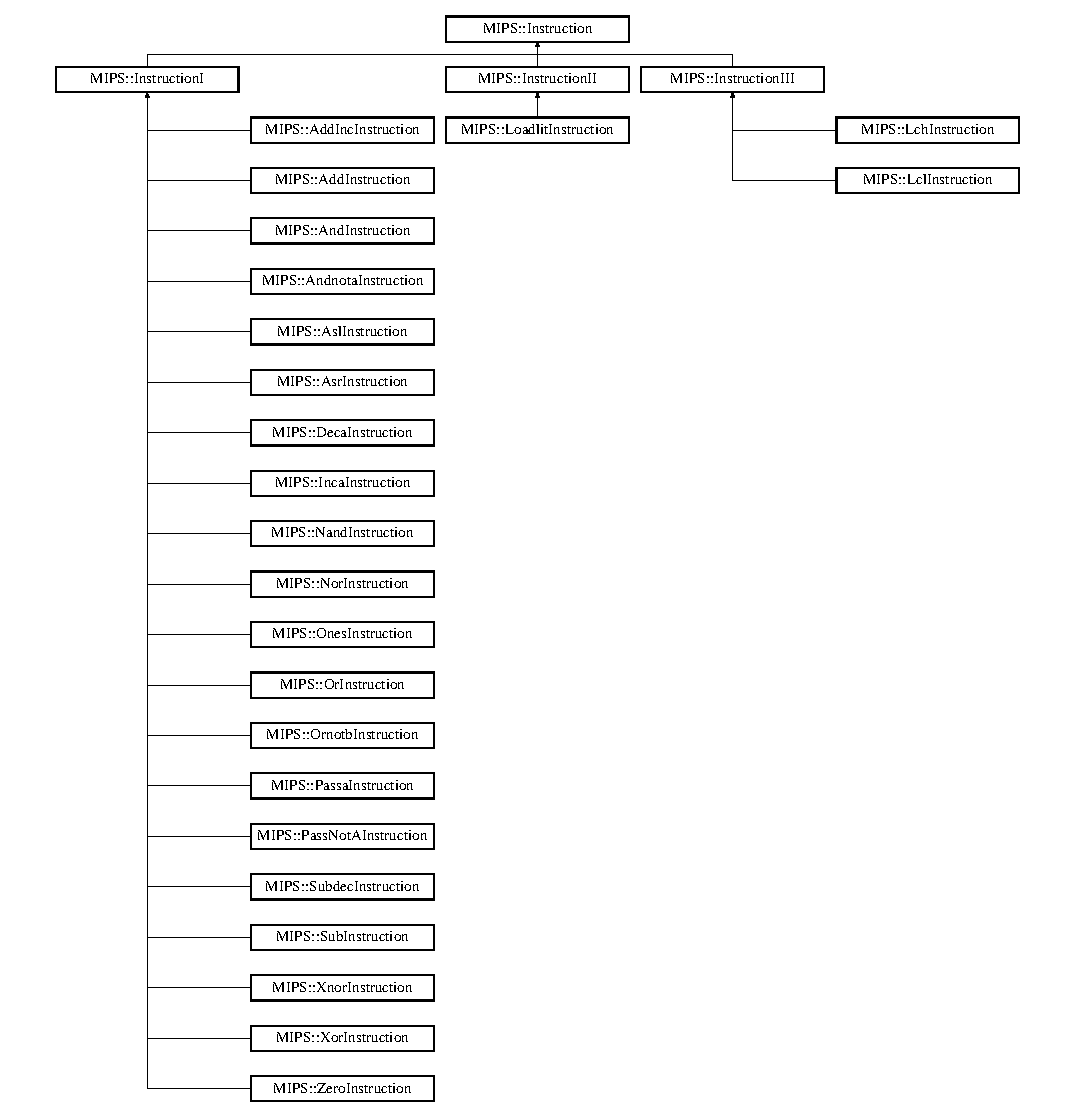
\includegraphics[height=8.099935cm]{classMIPS_1_1Instruction}
\end{center}
\end{figure}
\subsection*{Public Member Functions}
\begin{DoxyCompactItemize}
\item 
\hyperlink{classMIPS_1_1Instruction_ab99cb1c89cd950412585375681b1466d}{$\sim$\+Instruction} ()
\item 
virtual \hyperlink{core_8hpp_adc265a970bc35995b5879784bbb3f1b7}{bit16\+\_\+t} \hyperlink{classMIPS_1_1Instruction_a88668dfaf49dd8608f210ba13948d242}{execute} ()=0
\item 
virtual void \hyperlink{classMIPS_1_1Instruction_a7df847adef2997446ffca9b71c2f3112}{update\+Control} (\hyperlink{classMIPS_1_1ControlUnit}{Control\+Unit} \&control)
\end{DoxyCompactItemize}
\subsection*{Protected Attributes}
\begin{DoxyCompactItemize}
\item 
\hyperlink{core_8hpp_a6074bae122ae7b527864eec42c728c3c}{bit8\+\_\+t} \hyperlink{classMIPS_1_1Instruction_a45cc6808b5dde8a5d41067d148b55476}{opcode}
\item 
\hyperlink{core_8hpp_a6074bae122ae7b527864eec42c728c3c}{bit8\+\_\+t} \hyperlink{classMIPS_1_1Instruction_a78e2b55f80640b476e99ee54f5be068c}{zero}
\item 
\hyperlink{core_8hpp_a6074bae122ae7b527864eec42c728c3c}{bit8\+\_\+t} \hyperlink{classMIPS_1_1Instruction_ad13e93d52d4df49287f3e92711b3927f}{neg}
\item 
\hyperlink{core_8hpp_a6074bae122ae7b527864eec42c728c3c}{bit8\+\_\+t} \hyperlink{classMIPS_1_1Instruction_a9894219fb3f9f6d0c33959bf45bf8151}{carry}
\item 
\hyperlink{core_8hpp_a6074bae122ae7b527864eec42c728c3c}{bit8\+\_\+t} \hyperlink{classMIPS_1_1Instruction_a34c04dbd0f64117d7b19f8bf6e6cb87a}{overflow}
\end{DoxyCompactItemize}


\subsection{Detailed Description}
Classe abstrata responsável por representar qualquer instrução em uma arquitetura de 16 bits.

\begin{DoxyAuthor}{Author}
Matheus Nogueira 
\end{DoxyAuthor}


\subsection{Constructor \& Destructor Documentation}
\index{M\+I\+P\+S\+::\+Instruction@{M\+I\+P\+S\+::\+Instruction}!````~Instruction@{$\sim$\+Instruction}}
\index{````~Instruction@{$\sim$\+Instruction}!M\+I\+P\+S\+::\+Instruction@{M\+I\+P\+S\+::\+Instruction}}
\subsubsection[{\texorpdfstring{$\sim$\+Instruction()}{~Instruction()}}]{\setlength{\rightskip}{0pt plus 5cm}M\+I\+P\+S\+::\+Instruction\+::$\sim$\+Instruction (
\begin{DoxyParamCaption}
{}
\end{DoxyParamCaption}
)\hspace{0.3cm}{\ttfamily [inline]}}\hypertarget{classMIPS_1_1Instruction_ab99cb1c89cd950412585375681b1466d}{}\label{classMIPS_1_1Instruction_ab99cb1c89cd950412585375681b1466d}
Destroi a instrução. 

\subsection{Member Function Documentation}
\index{M\+I\+P\+S\+::\+Instruction@{M\+I\+P\+S\+::\+Instruction}!execute@{execute}}
\index{execute@{execute}!M\+I\+P\+S\+::\+Instruction@{M\+I\+P\+S\+::\+Instruction}}
\subsubsection[{\texorpdfstring{execute()=0}{execute()=0}}]{\setlength{\rightskip}{0pt plus 5cm}virtual {\bf bit16\+\_\+t} M\+I\+P\+S\+::\+Instruction\+::execute (
\begin{DoxyParamCaption}
{}
\end{DoxyParamCaption}
)\hspace{0.3cm}{\ttfamily [pure virtual]}}\hypertarget{classMIPS_1_1Instruction_a88668dfaf49dd8608f210ba13948d242}{}\label{classMIPS_1_1Instruction_a88668dfaf49dd8608f210ba13948d242}
Método abstrato que deverá ser invocado para que uma instrução seja executada pelo emulador.

\begin{DoxyReturn}{Returns}
resultado de saída da instrução. 
\end{DoxyReturn}


Implemented in \hyperlink{classMIPS_1_1InstructionI_ae60fca5801bf5415cdff06d2aa11764f}{M\+I\+P\+S\+::\+InstructionI}, \hyperlink{classMIPS_1_1InstructionVII_ab004a9cdc0efa7afacb964352abf3ee7}{M\+I\+P\+S\+::\+Instruction\+V\+II}, \hyperlink{classMIPS_1_1InstructionVI_a0a334d9d507fca448eaa7b0190c17531}{M\+I\+P\+S\+::\+Instruction\+VI}, \hyperlink{classMIPS_1_1InstructionII_aa014c5b0fe877746ca4db85c971a2e93}{M\+I\+P\+S\+::\+Instruction\+II}, \hyperlink{classMIPS_1_1InstructionIII_aee3071c23abc542e55b446abee766c5e}{M\+I\+P\+S\+::\+Instruction\+I\+II}, \hyperlink{classMIPS_1_1InstructionIV_ae9eeb2c1aa5392cc3e2d9f2d816b799c}{M\+I\+P\+S\+::\+Instruction\+IV}, \hyperlink{classMIPS_1_1InstructionV_a511d8ba098bcca95f1e91ff6616470ef}{M\+I\+P\+S\+::\+InstructionV}, \hyperlink{classMIPS_1_1LchInstruction_a6dad60c9189a1e84fd7c789b9642077d}{M\+I\+P\+S\+::\+Lch\+Instruction}, \hyperlink{classMIPS_1_1LclInstruction_a713c7c0e33c9df49f677abfd95f363db}{M\+I\+P\+S\+::\+Lcl\+Instruction}, \hyperlink{classMIPS_1_1LoadlitInstruction_a9f88a932bbbf31375da7686b449608e1}{M\+I\+P\+S\+::\+Loadlit\+Instruction}, \hyperlink{classMIPS_1_1AddInstruction_aa699dc00fdcd4250944f8afaa2fa89eb}{M\+I\+P\+S\+::\+Add\+Instruction}, \hyperlink{classMIPS_1_1AddIncInstruction_aa63fcaf17a9afc2f1b5d09a6291a70d6}{M\+I\+P\+S\+::\+Add\+Inc\+Instruction}, \hyperlink{classMIPS_1_1AndnotaInstruction_afdc3b2836318f4adaa32dfa3bcdf7c45}{M\+I\+P\+S\+::\+Andnota\+Instruction}, \hyperlink{classMIPS_1_1AslInstruction_adafc2d1f549cda9bdf757dc2bac03ca9}{M\+I\+P\+S\+::\+Asl\+Instruction}, \hyperlink{classMIPS_1_1AsrInstruction_aad46283e10517abf6bf5e527ca020d53}{M\+I\+P\+S\+::\+Asr\+Instruction}, \hyperlink{classMIPS_1_1DecaInstruction_a82c3d685d910d2c52163f5faa1750aca}{M\+I\+P\+S\+::\+Deca\+Instruction}, \hyperlink{classMIPS_1_1IncaInstruction_ac78e4a0b037ab4b6b419f4f5a34413c7}{M\+I\+P\+S\+::\+Inca\+Instruction}, \hyperlink{classMIPS_1_1NandInstruction_a2e0266ebee3819e7b4d9bfb44f0e70ac}{M\+I\+P\+S\+::\+Nand\+Instruction}, \hyperlink{classMIPS_1_1NorInstruction_a68bb5cc9920bd63229f4c16c4edb5ab6}{M\+I\+P\+S\+::\+Nor\+Instruction}, \hyperlink{classMIPS_1_1OnesInstruction_aeab25fd32df5c092d4f426371f3f1ff3}{M\+I\+P\+S\+::\+Ones\+Instruction}, \hyperlink{classMIPS_1_1PassaInstruction_ae23b43bfb84d2ef69fa25e50fb5b6072}{M\+I\+P\+S\+::\+Passa\+Instruction}, \hyperlink{classMIPS_1_1PassNotAInstruction_a30b9bdb1feac1adb44e70a3a0eb85cb4}{M\+I\+P\+S\+::\+Pass\+Not\+A\+Instruction}, \hyperlink{classMIPS_1_1SubInstruction_a2b10f6bfda0e7d9651600b530cfccf62}{M\+I\+P\+S\+::\+Sub\+Instruction}, \hyperlink{classMIPS_1_1XnorInstruction_a4b5ae9a875883902c0ed1e237e753f31}{M\+I\+P\+S\+::\+Xnor\+Instruction}, \hyperlink{classMIPS_1_1XorInstruction_aaebc7dc8723627871ba2caf85f01fbea}{M\+I\+P\+S\+::\+Xor\+Instruction}, \hyperlink{classMIPS_1_1ZeroInstruction_a9596a96b4bf7a51672ab14386d111bad}{M\+I\+P\+S\+::\+Zero\+Instruction}, \hyperlink{classMIPS_1_1JtZeroInstruction_a8a56439dd5df5fcf00344304b8409e45}{M\+I\+P\+S\+::\+Jt\+Zero\+Instruction}, \hyperlink{classMIPS_1_1SubdecInstruction_a6d9e86774b950a584b60d9a48402af2a}{M\+I\+P\+S\+::\+Subdec\+Instruction}, \hyperlink{classMIPS_1_1JumpInstruction_a843961af93d20e35dd1fab6bf341e16e}{M\+I\+P\+S\+::\+Jump\+Instruction}, \hyperlink{classMIPS_1_1AndInstruction_a24b2fdb68ff022275db4181e502b7a48}{M\+I\+P\+S\+::\+And\+Instruction}, \hyperlink{classMIPS_1_1OrInstruction_a89859e0bcb3e5ed7f1c53f33f627f041}{M\+I\+P\+S\+::\+Or\+Instruction}, and \hyperlink{classMIPS_1_1OrnotbInstruction_a47aac4ac3ef0ee8c6a694189f26bd80e}{M\+I\+P\+S\+::\+Ornotb\+Instruction}.

\index{M\+I\+P\+S\+::\+Instruction@{M\+I\+P\+S\+::\+Instruction}!update\+Control@{update\+Control}}
\index{update\+Control@{update\+Control}!M\+I\+P\+S\+::\+Instruction@{M\+I\+P\+S\+::\+Instruction}}
\subsubsection[{\texorpdfstring{update\+Control(\+Control\+Unit \&control)}{updateControl(ControlUnit &control)}}]{\setlength{\rightskip}{0pt plus 5cm}virtual void M\+I\+P\+S\+::\+Instruction\+::update\+Control (
\begin{DoxyParamCaption}
\item[{{\bf Control\+Unit} \&}]{control}
\end{DoxyParamCaption}
)\hspace{0.3cm}{\ttfamily [inline]}, {\ttfamily [virtual]}}\hypertarget{classMIPS_1_1Instruction_a7df847adef2997446ffca9b71c2f3112}{}\label{classMIPS_1_1Instruction_a7df847adef2997446ffca9b71c2f3112}
Método utilizado para atualizar os sinais de controle do processador.


\begin{DoxyParams}{Parameters}
{\em control} & unidade de controle do processador. \\
\hline
\end{DoxyParams}


\subsection{Member Data Documentation}
\index{M\+I\+P\+S\+::\+Instruction@{M\+I\+P\+S\+::\+Instruction}!carry@{carry}}
\index{carry@{carry}!M\+I\+P\+S\+::\+Instruction@{M\+I\+P\+S\+::\+Instruction}}
\subsubsection[{\texorpdfstring{carry}{carry}}]{\setlength{\rightskip}{0pt plus 5cm}{\bf bit8\+\_\+t} M\+I\+P\+S\+::\+Instruction\+::carry\hspace{0.3cm}{\ttfamily [protected]}}\hypertarget{classMIPS_1_1Instruction_a9894219fb3f9f6d0c33959bf45bf8151}{}\label{classMIPS_1_1Instruction_a9894219fb3f9f6d0c33959bf45bf8151}
Flag de carry. \index{M\+I\+P\+S\+::\+Instruction@{M\+I\+P\+S\+::\+Instruction}!neg@{neg}}
\index{neg@{neg}!M\+I\+P\+S\+::\+Instruction@{M\+I\+P\+S\+::\+Instruction}}
\subsubsection[{\texorpdfstring{neg}{neg}}]{\setlength{\rightskip}{0pt plus 5cm}{\bf bit8\+\_\+t} M\+I\+P\+S\+::\+Instruction\+::neg\hspace{0.3cm}{\ttfamily [protected]}}\hypertarget{classMIPS_1_1Instruction_ad13e93d52d4df49287f3e92711b3927f}{}\label{classMIPS_1_1Instruction_ad13e93d52d4df49287f3e92711b3927f}
Flag de negativo \index{M\+I\+P\+S\+::\+Instruction@{M\+I\+P\+S\+::\+Instruction}!opcode@{opcode}}
\index{opcode@{opcode}!M\+I\+P\+S\+::\+Instruction@{M\+I\+P\+S\+::\+Instruction}}
\subsubsection[{\texorpdfstring{opcode}{opcode}}]{\setlength{\rightskip}{0pt plus 5cm}{\bf bit8\+\_\+t} M\+I\+P\+S\+::\+Instruction\+::opcode\hspace{0.3cm}{\ttfamily [protected]}}\hypertarget{classMIPS_1_1Instruction_a45cc6808b5dde8a5d41067d148b55476}{}\label{classMIPS_1_1Instruction_a45cc6808b5dde8a5d41067d148b55476}
Código da operação (opcode) da instrução. \index{M\+I\+P\+S\+::\+Instruction@{M\+I\+P\+S\+::\+Instruction}!overflow@{overflow}}
\index{overflow@{overflow}!M\+I\+P\+S\+::\+Instruction@{M\+I\+P\+S\+::\+Instruction}}
\subsubsection[{\texorpdfstring{overflow}{overflow}}]{\setlength{\rightskip}{0pt plus 5cm}{\bf bit8\+\_\+t} M\+I\+P\+S\+::\+Instruction\+::overflow\hspace{0.3cm}{\ttfamily [protected]}}\hypertarget{classMIPS_1_1Instruction_a34c04dbd0f64117d7b19f8bf6e6cb87a}{}\label{classMIPS_1_1Instruction_a34c04dbd0f64117d7b19f8bf6e6cb87a}
flag de overflow \index{M\+I\+P\+S\+::\+Instruction@{M\+I\+P\+S\+::\+Instruction}!zero@{zero}}
\index{zero@{zero}!M\+I\+P\+S\+::\+Instruction@{M\+I\+P\+S\+::\+Instruction}}
\subsubsection[{\texorpdfstring{zero}{zero}}]{\setlength{\rightskip}{0pt plus 5cm}{\bf bit8\+\_\+t} M\+I\+P\+S\+::\+Instruction\+::zero\hspace{0.3cm}{\ttfamily [protected]}}\hypertarget{classMIPS_1_1Instruction_a78e2b55f80640b476e99ee54f5be068c}{}\label{classMIPS_1_1Instruction_a78e2b55f80640b476e99ee54f5be068c}
Flag de zero. 

The documentation for this class was generated from the following file\+:\begin{DoxyCompactItemize}
\item 
include/mips/instructions/\hyperlink{instruction_8hpp}{instruction.\+hpp}\end{DoxyCompactItemize}

\hypertarget{classMIPS_1_1InstructionDecoder}{}\section{M\+I\+PS\+:\+:Instruction\+Decoder Class Reference}
\label{classMIPS_1_1InstructionDecoder}\index{M\+I\+P\+S\+::\+Instruction\+Decoder@{M\+I\+P\+S\+::\+Instruction\+Decoder}}


{\ttfamily \#include $<$instruction\+\_\+decoder.\+hpp$>$}

\subsection*{Public Member Functions}
\begin{DoxyCompactItemize}
\item 
\hyperlink{classMIPS_1_1InstructionDecoder_a81c1e3f43edf65ca86dba43a9090c9fc}{Instruction\+Decoder} (\hyperlink{classMIPS_1_1RegisterBank}{Register\+Bank} \&bank)
\item 
\hyperlink{classMIPS_1_1InstructionDecoder_a148a38deb0745a55bbd927d186f93c89}{$\sim$\+Instruction\+Decoder} ()
\item 
\hyperlink{classMIPS_1_1Instruction}{Instruction} $\ast$ \hyperlink{classMIPS_1_1InstructionDecoder_adf51f7da13d3256b60d99384cdc4af63}{decode} (\hyperlink{core_8hpp_aa514fd240a0e29abb2a2e4c805d7f1a4}{instruction\+\_\+t} instruction)
\item 
\hyperlink{core_8hpp_a6074bae122ae7b527864eec42c728c3c}{bit8\+\_\+t} \hyperlink{classMIPS_1_1InstructionDecoder_a9ba2a37411b5e8d4e7b03c4d5b50399b}{get\+O\+P\+Code} (\hyperlink{core_8hpp_aa514fd240a0e29abb2a2e4c805d7f1a4}{instruction\+\_\+t} instruction)
\item 
\hyperlink{core_8hpp_a6074bae122ae7b527864eec42c728c3c}{bit8\+\_\+t} \hyperlink{classMIPS_1_1InstructionDecoder_a557dfb2243be5d1a0a369c333817fa86}{get\+Rs} (\hyperlink{core_8hpp_aa514fd240a0e29abb2a2e4c805d7f1a4}{instruction\+\_\+t} instruction)
\item 
\hyperlink{core_8hpp_a6074bae122ae7b527864eec42c728c3c}{bit8\+\_\+t} \hyperlink{classMIPS_1_1InstructionDecoder_a4da42498cc12ddcc041b42bacbc3b3a1}{get\+Rt} (\hyperlink{core_8hpp_aa514fd240a0e29abb2a2e4c805d7f1a4}{instruction\+\_\+t} instruction)
\item 
\hyperlink{core_8hpp_a6074bae122ae7b527864eec42c728c3c}{bit8\+\_\+t} \hyperlink{classMIPS_1_1InstructionDecoder_a493aeaf3390fb5821596ef3efc22e65b}{get\+Rd} (\hyperlink{core_8hpp_aa514fd240a0e29abb2a2e4c805d7f1a4}{instruction\+\_\+t} instruction)
\item 
\hyperlink{core_8hpp_a6074bae122ae7b527864eec42c728c3c}{bit8\+\_\+t} \hyperlink{classMIPS_1_1InstructionDecoder_aa7148e0ad81662725be7203837a4e46c}{get\+Funct} (\hyperlink{core_8hpp_aa514fd240a0e29abb2a2e4c805d7f1a4}{instruction\+\_\+t} instruction)
\item 
\hyperlink{core_8hpp_a6074bae122ae7b527864eec42c728c3c}{bit8\+\_\+t} \hyperlink{classMIPS_1_1InstructionDecoder_ab0e5dc987aa8c65f78aaba3ba242673b}{get\+Jump\+Op} (\hyperlink{core_8hpp_aa514fd240a0e29abb2a2e4c805d7f1a4}{instruction\+\_\+t} instruction)
\item 
\hyperlink{core_8hpp_a6074bae122ae7b527864eec42c728c3c}{bit8\+\_\+t} \hyperlink{classMIPS_1_1InstructionDecoder_afef4b26e3420aa5a32473593868703d2}{get\+Jump\+Cond} (\hyperlink{core_8hpp_aa514fd240a0e29abb2a2e4c805d7f1a4}{instruction\+\_\+t} instruction)
\item 
\hyperlink{core_8hpp_adc265a970bc35995b5879784bbb3f1b7}{bit16\+\_\+t} \hyperlink{classMIPS_1_1InstructionDecoder_a09ba48d5683432c3a303b8c42367755f}{get\+Offset} (\hyperlink{core_8hpp_aa514fd240a0e29abb2a2e4c805d7f1a4}{instruction\+\_\+t} instruction, \hyperlink{core_8hpp_a6074bae122ae7b527864eec42c728c3c}{bit8\+\_\+t} size=8)
\end{DoxyCompactItemize}
\subsection*{Protected Attributes}
\begin{DoxyCompactItemize}
\item 
\hyperlink{classMIPS_1_1RegisterBank}{Register\+Bank} \& \hyperlink{classMIPS_1_1InstructionDecoder_a6796453642fca3384868a9539656ab45}{register\+Bank}
\end{DoxyCompactItemize}


\subsection{Detailed Description}
Classe responsável por receber uma instrução em binário e instanciar uma instrução do emulador que pode executar a instrução equivalente.

\begin{DoxyAuthor}{Author}
Matheus Nogueira 
\end{DoxyAuthor}


\subsection{Constructor \& Destructor Documentation}
\index{M\+I\+P\+S\+::\+Instruction\+Decoder@{M\+I\+P\+S\+::\+Instruction\+Decoder}!Instruction\+Decoder@{Instruction\+Decoder}}
\index{Instruction\+Decoder@{Instruction\+Decoder}!M\+I\+P\+S\+::\+Instruction\+Decoder@{M\+I\+P\+S\+::\+Instruction\+Decoder}}
\subsubsection[{\texorpdfstring{Instruction\+Decoder(\+Register\+Bank \&bank)}{InstructionDecoder(RegisterBank &bank)}}]{\setlength{\rightskip}{0pt plus 5cm}M\+I\+P\+S\+::\+Instruction\+Decoder\+::\+Instruction\+Decoder (
\begin{DoxyParamCaption}
\item[{{\bf Register\+Bank} \&}]{bank}
\end{DoxyParamCaption}
)}\hypertarget{classMIPS_1_1InstructionDecoder_a81c1e3f43edf65ca86dba43a9090c9fc}{}\label{classMIPS_1_1InstructionDecoder_a81c1e3f43edf65ca86dba43a9090c9fc}
Cria um novo decodificador de instruções.


\begin{DoxyParams}{Parameters}
{\em bank} & banco de registradores usado. \\
\hline
\end{DoxyParams}
\index{M\+I\+P\+S\+::\+Instruction\+Decoder@{M\+I\+P\+S\+::\+Instruction\+Decoder}!````~Instruction\+Decoder@{$\sim$\+Instruction\+Decoder}}
\index{````~Instruction\+Decoder@{$\sim$\+Instruction\+Decoder}!M\+I\+P\+S\+::\+Instruction\+Decoder@{M\+I\+P\+S\+::\+Instruction\+Decoder}}
\subsubsection[{\texorpdfstring{$\sim$\+Instruction\+Decoder()}{~InstructionDecoder()}}]{\setlength{\rightskip}{0pt plus 5cm}M\+I\+P\+S\+::\+Instruction\+Decoder\+::$\sim$\+Instruction\+Decoder (
\begin{DoxyParamCaption}
{}
\end{DoxyParamCaption}
)}\hypertarget{classMIPS_1_1InstructionDecoder_a148a38deb0745a55bbd927d186f93c89}{}\label{classMIPS_1_1InstructionDecoder_a148a38deb0745a55bbd927d186f93c89}
Destroi o decodificador de instruções. 

\subsection{Member Function Documentation}
\index{M\+I\+P\+S\+::\+Instruction\+Decoder@{M\+I\+P\+S\+::\+Instruction\+Decoder}!decode@{decode}}
\index{decode@{decode}!M\+I\+P\+S\+::\+Instruction\+Decoder@{M\+I\+P\+S\+::\+Instruction\+Decoder}}
\subsubsection[{\texorpdfstring{decode(instruction\+\_\+t instruction)}{decode(instruction_t instruction)}}]{\setlength{\rightskip}{0pt plus 5cm}{\bf Instruction}$\ast$ M\+I\+P\+S\+::\+Instruction\+Decoder\+::decode (
\begin{DoxyParamCaption}
\item[{{\bf instruction\+\_\+t}}]{instruction}
\end{DoxyParamCaption}
)}\hypertarget{classMIPS_1_1InstructionDecoder_adf51f7da13d3256b60d99384cdc4af63}{}\label{classMIPS_1_1InstructionDecoder_adf51f7da13d3256b60d99384cdc4af63}
Decodifica uma instrução em binário e cria uma instrução do emulador que realize a operação equivalente.


\begin{DoxyParams}{Parameters}
{\em instruction} & instrução 16 bits em binário. \\
\hline
\end{DoxyParams}
\begin{DoxyReturn}{Returns}
ponteiro para a instrução criada pelo emulador. 
\end{DoxyReturn}
\index{M\+I\+P\+S\+::\+Instruction\+Decoder@{M\+I\+P\+S\+::\+Instruction\+Decoder}!get\+Funct@{get\+Funct}}
\index{get\+Funct@{get\+Funct}!M\+I\+P\+S\+::\+Instruction\+Decoder@{M\+I\+P\+S\+::\+Instruction\+Decoder}}
\subsubsection[{\texorpdfstring{get\+Funct(instruction\+\_\+t instruction)}{getFunct(instruction_t instruction)}}]{\setlength{\rightskip}{0pt plus 5cm}{\bf bit8\+\_\+t} M\+I\+P\+S\+::\+Instruction\+Decoder\+::get\+Funct (
\begin{DoxyParamCaption}
\item[{{\bf instruction\+\_\+t}}]{instruction}
\end{DoxyParamCaption}
)}\hypertarget{classMIPS_1_1InstructionDecoder_aa7148e0ad81662725be7203837a4e46c}{}\label{classMIPS_1_1InstructionDecoder_aa7148e0ad81662725be7203837a4e46c}
Função que recupera o valor do funct da instrução.


\begin{DoxyParams}{Parameters}
{\em instruction} & instrução binária de 16 bits. \\
\hline
\end{DoxyParams}
\begin{DoxyReturn}{Returns}
valor do funct 
\end{DoxyReturn}
\index{M\+I\+P\+S\+::\+Instruction\+Decoder@{M\+I\+P\+S\+::\+Instruction\+Decoder}!get\+Jump\+Cond@{get\+Jump\+Cond}}
\index{get\+Jump\+Cond@{get\+Jump\+Cond}!M\+I\+P\+S\+::\+Instruction\+Decoder@{M\+I\+P\+S\+::\+Instruction\+Decoder}}
\subsubsection[{\texorpdfstring{get\+Jump\+Cond(instruction\+\_\+t instruction)}{getJumpCond(instruction_t instruction)}}]{\setlength{\rightskip}{0pt plus 5cm}{\bf bit8\+\_\+t} M\+I\+P\+S\+::\+Instruction\+Decoder\+::get\+Jump\+Cond (
\begin{DoxyParamCaption}
\item[{{\bf instruction\+\_\+t}}]{instruction}
\end{DoxyParamCaption}
)}\hypertarget{classMIPS_1_1InstructionDecoder_afef4b26e3420aa5a32473593868703d2}{}\label{classMIPS_1_1InstructionDecoder_afef4b26e3420aa5a32473593868703d2}
Pega o valor de condição do jump.


\begin{DoxyParams}{Parameters}
{\em instruction} & instrução binária de 16 bits. \\
\hline
\end{DoxyParams}
\begin{DoxyReturn}{Returns}
valor do cond. 
\end{DoxyReturn}
\index{M\+I\+P\+S\+::\+Instruction\+Decoder@{M\+I\+P\+S\+::\+Instruction\+Decoder}!get\+Jump\+Op@{get\+Jump\+Op}}
\index{get\+Jump\+Op@{get\+Jump\+Op}!M\+I\+P\+S\+::\+Instruction\+Decoder@{M\+I\+P\+S\+::\+Instruction\+Decoder}}
\subsubsection[{\texorpdfstring{get\+Jump\+Op(instruction\+\_\+t instruction)}{getJumpOp(instruction_t instruction)}}]{\setlength{\rightskip}{0pt plus 5cm}{\bf bit8\+\_\+t} M\+I\+P\+S\+::\+Instruction\+Decoder\+::get\+Jump\+Op (
\begin{DoxyParamCaption}
\item[{{\bf instruction\+\_\+t}}]{instruction}
\end{DoxyParamCaption}
)}\hypertarget{classMIPS_1_1InstructionDecoder_ab0e5dc987aa8c65f78aaba3ba242673b}{}\label{classMIPS_1_1InstructionDecoder_ab0e5dc987aa8c65f78aaba3ba242673b}
Pega o valor do codigo de diferenciação dos jumps.


\begin{DoxyParams}{Parameters}
{\em instruction} & instrução binária de 16 bits. \\
\hline
\end{DoxyParams}
\begin{DoxyReturn}{Returns}
valor de diferenciação. 
\end{DoxyReturn}
\index{M\+I\+P\+S\+::\+Instruction\+Decoder@{M\+I\+P\+S\+::\+Instruction\+Decoder}!get\+Offset@{get\+Offset}}
\index{get\+Offset@{get\+Offset}!M\+I\+P\+S\+::\+Instruction\+Decoder@{M\+I\+P\+S\+::\+Instruction\+Decoder}}
\subsubsection[{\texorpdfstring{get\+Offset(instruction\+\_\+t instruction, bit8\+\_\+t size=8)}{getOffset(instruction_t instruction, bit8_t size=8)}}]{\setlength{\rightskip}{0pt plus 5cm}{\bf bit16\+\_\+t} M\+I\+P\+S\+::\+Instruction\+Decoder\+::get\+Offset (
\begin{DoxyParamCaption}
\item[{{\bf instruction\+\_\+t}}]{instruction, }
\item[{{\bf bit8\+\_\+t}}]{size = {\ttfamily 8}}
\end{DoxyParamCaption}
)}\hypertarget{classMIPS_1_1InstructionDecoder_a09ba48d5683432c3a303b8c42367755f}{}\label{classMIPS_1_1InstructionDecoder_a09ba48d5683432c3a303b8c42367755f}
Função que recupera o valor do offset da instrução.


\begin{DoxyParams}{Parameters}
{\em instruction} & instrução binária de 16 bits. \\
\hline
{\em size} & número de bits de offset \\
\hline
\end{DoxyParams}
\begin{DoxyReturn}{Returns}
valor do offset. 
\end{DoxyReturn}
\index{M\+I\+P\+S\+::\+Instruction\+Decoder@{M\+I\+P\+S\+::\+Instruction\+Decoder}!get\+O\+P\+Code@{get\+O\+P\+Code}}
\index{get\+O\+P\+Code@{get\+O\+P\+Code}!M\+I\+P\+S\+::\+Instruction\+Decoder@{M\+I\+P\+S\+::\+Instruction\+Decoder}}
\subsubsection[{\texorpdfstring{get\+O\+P\+Code(instruction\+\_\+t instruction)}{getOPCode(instruction_t instruction)}}]{\setlength{\rightskip}{0pt plus 5cm}{\bf bit8\+\_\+t} M\+I\+P\+S\+::\+Instruction\+Decoder\+::get\+O\+P\+Code (
\begin{DoxyParamCaption}
\item[{{\bf instruction\+\_\+t}}]{instruction}
\end{DoxyParamCaption}
)}\hypertarget{classMIPS_1_1InstructionDecoder_a9ba2a37411b5e8d4e7b03c4d5b50399b}{}\label{classMIPS_1_1InstructionDecoder_a9ba2a37411b5e8d4e7b03c4d5b50399b}
Método responsável por recuperar o código de operação (opcode) de uma instrução.


\begin{DoxyParams}{Parameters}
{\em instruction} & instrução de onde o opcode deve ser extraído. \\
\hline
\end{DoxyParams}
\begin{DoxyReturn}{Returns}
opcode da instrução. 
\end{DoxyReturn}
\index{M\+I\+P\+S\+::\+Instruction\+Decoder@{M\+I\+P\+S\+::\+Instruction\+Decoder}!get\+Rd@{get\+Rd}}
\index{get\+Rd@{get\+Rd}!M\+I\+P\+S\+::\+Instruction\+Decoder@{M\+I\+P\+S\+::\+Instruction\+Decoder}}
\subsubsection[{\texorpdfstring{get\+Rd(instruction\+\_\+t instruction)}{getRd(instruction_t instruction)}}]{\setlength{\rightskip}{0pt plus 5cm}{\bf bit8\+\_\+t} M\+I\+P\+S\+::\+Instruction\+Decoder\+::get\+Rd (
\begin{DoxyParamCaption}
\item[{{\bf instruction\+\_\+t}}]{instruction}
\end{DoxyParamCaption}
)}\hypertarget{classMIPS_1_1InstructionDecoder_a493aeaf3390fb5821596ef3efc22e65b}{}\label{classMIPS_1_1InstructionDecoder_a493aeaf3390fb5821596ef3efc22e65b}
Função que recupera o endereço do registrador destination (Rd) da instrução.


\begin{DoxyParams}{Parameters}
{\em instruction} & instrução binária de 16 bits. \\
\hline
\end{DoxyParams}
\begin{DoxyReturn}{Returns}
endereço do registrador destination. 
\end{DoxyReturn}
\index{M\+I\+P\+S\+::\+Instruction\+Decoder@{M\+I\+P\+S\+::\+Instruction\+Decoder}!get\+Rs@{get\+Rs}}
\index{get\+Rs@{get\+Rs}!M\+I\+P\+S\+::\+Instruction\+Decoder@{M\+I\+P\+S\+::\+Instruction\+Decoder}}
\subsubsection[{\texorpdfstring{get\+Rs(instruction\+\_\+t instruction)}{getRs(instruction_t instruction)}}]{\setlength{\rightskip}{0pt plus 5cm}{\bf bit8\+\_\+t} M\+I\+P\+S\+::\+Instruction\+Decoder\+::get\+Rs (
\begin{DoxyParamCaption}
\item[{{\bf instruction\+\_\+t}}]{instruction}
\end{DoxyParamCaption}
)}\hypertarget{classMIPS_1_1InstructionDecoder_a557dfb2243be5d1a0a369c333817fa86}{}\label{classMIPS_1_1InstructionDecoder_a557dfb2243be5d1a0a369c333817fa86}
Função que recupera o endereço do registrador source (Rs) da instrução.


\begin{DoxyParams}{Parameters}
{\em instruction} & instrução binária de 16 bits. \\
\hline
\end{DoxyParams}
\begin{DoxyReturn}{Returns}
endereço do registrador source. 
\end{DoxyReturn}
\index{M\+I\+P\+S\+::\+Instruction\+Decoder@{M\+I\+P\+S\+::\+Instruction\+Decoder}!get\+Rt@{get\+Rt}}
\index{get\+Rt@{get\+Rt}!M\+I\+P\+S\+::\+Instruction\+Decoder@{M\+I\+P\+S\+::\+Instruction\+Decoder}}
\subsubsection[{\texorpdfstring{get\+Rt(instruction\+\_\+t instruction)}{getRt(instruction_t instruction)}}]{\setlength{\rightskip}{0pt plus 5cm}{\bf bit8\+\_\+t} M\+I\+P\+S\+::\+Instruction\+Decoder\+::get\+Rt (
\begin{DoxyParamCaption}
\item[{{\bf instruction\+\_\+t}}]{instruction}
\end{DoxyParamCaption}
)}\hypertarget{classMIPS_1_1InstructionDecoder_a4da42498cc12ddcc041b42bacbc3b3a1}{}\label{classMIPS_1_1InstructionDecoder_a4da42498cc12ddcc041b42bacbc3b3a1}
Função que recupera o endereço do registrador target (Rt) da instrução.


\begin{DoxyParams}{Parameters}
{\em instruction} & instrução binária de 16 bits. \\
\hline
\end{DoxyParams}
\begin{DoxyReturn}{Returns}
endereço do registrador target. 
\end{DoxyReturn}


\subsection{Member Data Documentation}
\index{M\+I\+P\+S\+::\+Instruction\+Decoder@{M\+I\+P\+S\+::\+Instruction\+Decoder}!register\+Bank@{register\+Bank}}
\index{register\+Bank@{register\+Bank}!M\+I\+P\+S\+::\+Instruction\+Decoder@{M\+I\+P\+S\+::\+Instruction\+Decoder}}
\subsubsection[{\texorpdfstring{register\+Bank}{registerBank}}]{\setlength{\rightskip}{0pt plus 5cm}{\bf Register\+Bank}\& M\+I\+P\+S\+::\+Instruction\+Decoder\+::register\+Bank\hspace{0.3cm}{\ttfamily [protected]}}\hypertarget{classMIPS_1_1InstructionDecoder_a6796453642fca3384868a9539656ab45}{}\label{classMIPS_1_1InstructionDecoder_a6796453642fca3384868a9539656ab45}
Banco de registradores do decodificador. 

The documentation for this class was generated from the following file\+:\begin{DoxyCompactItemize}
\item 
include/mips/decoder/\hyperlink{instruction__decoder_8hpp}{instruction\+\_\+decoder.\+hpp}\end{DoxyCompactItemize}

\hypertarget{classMIPS_1_1InstructionFinder}{}\section{M\+I\+PS\+:\+:Instruction\+Finder Class Reference}
\label{classMIPS_1_1InstructionFinder}\index{M\+I\+P\+S\+::\+Instruction\+Finder@{M\+I\+P\+S\+::\+Instruction\+Finder}}


{\ttfamily \#include $<$instruction\+\_\+finder.\+hpp$>$}

\subsection*{Public Member Functions}
\begin{DoxyCompactItemize}
\item 
\hyperlink{classMIPS_1_1InstructionFinder_abda3d40a1a5f355991fc5f135a826b96}{Instruction\+Finder} (\hyperlink{classMIPS_1_1Memory}{Memory} \&memory\+Unit, \hyperlink{classMIPS_1_1RegisterBank}{Register\+Bank} \&bank)
\item 
\hyperlink{classMIPS_1_1InstructionFinder_a9079f27b5bca86251ee97196abe20cec}{$\sim$\+Instruction\+Finder} ()
\item 
\hyperlink{core_8hpp_aa514fd240a0e29abb2a2e4c805d7f1a4}{instruction\+\_\+t} \hyperlink{classMIPS_1_1InstructionFinder_a73a242cbe648c2d5e1cd0dd9342f798a}{get\+Next} ()
\end{DoxyCompactItemize}


\subsection{Detailed Description}
Classe que representa a unidade de busca de instruções na memória.

\begin{DoxyAuthor}{Author}
Matheus Nogueira 
\end{DoxyAuthor}


\subsection{Constructor \& Destructor Documentation}
\index{M\+I\+P\+S\+::\+Instruction\+Finder@{M\+I\+P\+S\+::\+Instruction\+Finder}!Instruction\+Finder@{Instruction\+Finder}}
\index{Instruction\+Finder@{Instruction\+Finder}!M\+I\+P\+S\+::\+Instruction\+Finder@{M\+I\+P\+S\+::\+Instruction\+Finder}}
\subsubsection[{\texorpdfstring{Instruction\+Finder(\+Memory \&memory\+Unit, Register\+Bank \&bank)}{InstructionFinder(Memory &memoryUnit, RegisterBank &bank)}}]{\setlength{\rightskip}{0pt plus 5cm}M\+I\+P\+S\+::\+Instruction\+Finder\+::\+Instruction\+Finder (
\begin{DoxyParamCaption}
\item[{{\bf Memory} \&}]{memory\+Unit, }
\item[{{\bf Register\+Bank} \&}]{bank}
\end{DoxyParamCaption}
)}\hypertarget{classMIPS_1_1InstructionFinder_abda3d40a1a5f355991fc5f135a826b96}{}\label{classMIPS_1_1InstructionFinder_abda3d40a1a5f355991fc5f135a826b96}
Cria uma nova unidade para busca de instruções. \index{M\+I\+P\+S\+::\+Instruction\+Finder@{M\+I\+P\+S\+::\+Instruction\+Finder}!````~Instruction\+Finder@{$\sim$\+Instruction\+Finder}}
\index{````~Instruction\+Finder@{$\sim$\+Instruction\+Finder}!M\+I\+P\+S\+::\+Instruction\+Finder@{M\+I\+P\+S\+::\+Instruction\+Finder}}
\subsubsection[{\texorpdfstring{$\sim$\+Instruction\+Finder()}{~InstructionFinder()}}]{\setlength{\rightskip}{0pt plus 5cm}M\+I\+P\+S\+::\+Instruction\+Finder\+::$\sim$\+Instruction\+Finder (
\begin{DoxyParamCaption}
{}
\end{DoxyParamCaption}
)}\hypertarget{classMIPS_1_1InstructionFinder_a9079f27b5bca86251ee97196abe20cec}{}\label{classMIPS_1_1InstructionFinder_a9079f27b5bca86251ee97196abe20cec}
Destroi a unidade de busca de instruções. 

\subsection{Member Function Documentation}
\index{M\+I\+P\+S\+::\+Instruction\+Finder@{M\+I\+P\+S\+::\+Instruction\+Finder}!get\+Next@{get\+Next}}
\index{get\+Next@{get\+Next}!M\+I\+P\+S\+::\+Instruction\+Finder@{M\+I\+P\+S\+::\+Instruction\+Finder}}
\subsubsection[{\texorpdfstring{get\+Next()}{getNext()}}]{\setlength{\rightskip}{0pt plus 5cm}{\bf instruction\+\_\+t} M\+I\+P\+S\+::\+Instruction\+Finder\+::get\+Next (
\begin{DoxyParamCaption}
{}
\end{DoxyParamCaption}
)}\hypertarget{classMIPS_1_1InstructionFinder_a73a242cbe648c2d5e1cd0dd9342f798a}{}\label{classMIPS_1_1InstructionFinder_a73a242cbe648c2d5e1cd0dd9342f798a}
Retorna a próxima instrução a ser executada, utilizando o registrador PC para identificá-\/la.

\begin{DoxyReturn}{Returns}
próxima instrução a ser executada. 
\end{DoxyReturn}


The documentation for this class was generated from the following file\+:\begin{DoxyCompactItemize}
\item 
include/mips/units/\hyperlink{instruction__finder_8hpp}{instruction\+\_\+finder.\+hpp}\end{DoxyCompactItemize}

\hypertarget{classMIPS_1_1InstructionI}{}\section{M\+I\+PS\+:\+:InstructionI Class Reference}
\label{classMIPS_1_1InstructionI}\index{M\+I\+P\+S\+::\+InstructionI@{M\+I\+P\+S\+::\+InstructionI}}


{\ttfamily \#include $<$instruction\+\_\+\+I.\+hpp$>$}

Inheritance diagram for M\+I\+PS\+:\+:InstructionI\+:\begin{figure}[H]
\begin{center}
\leavevmode
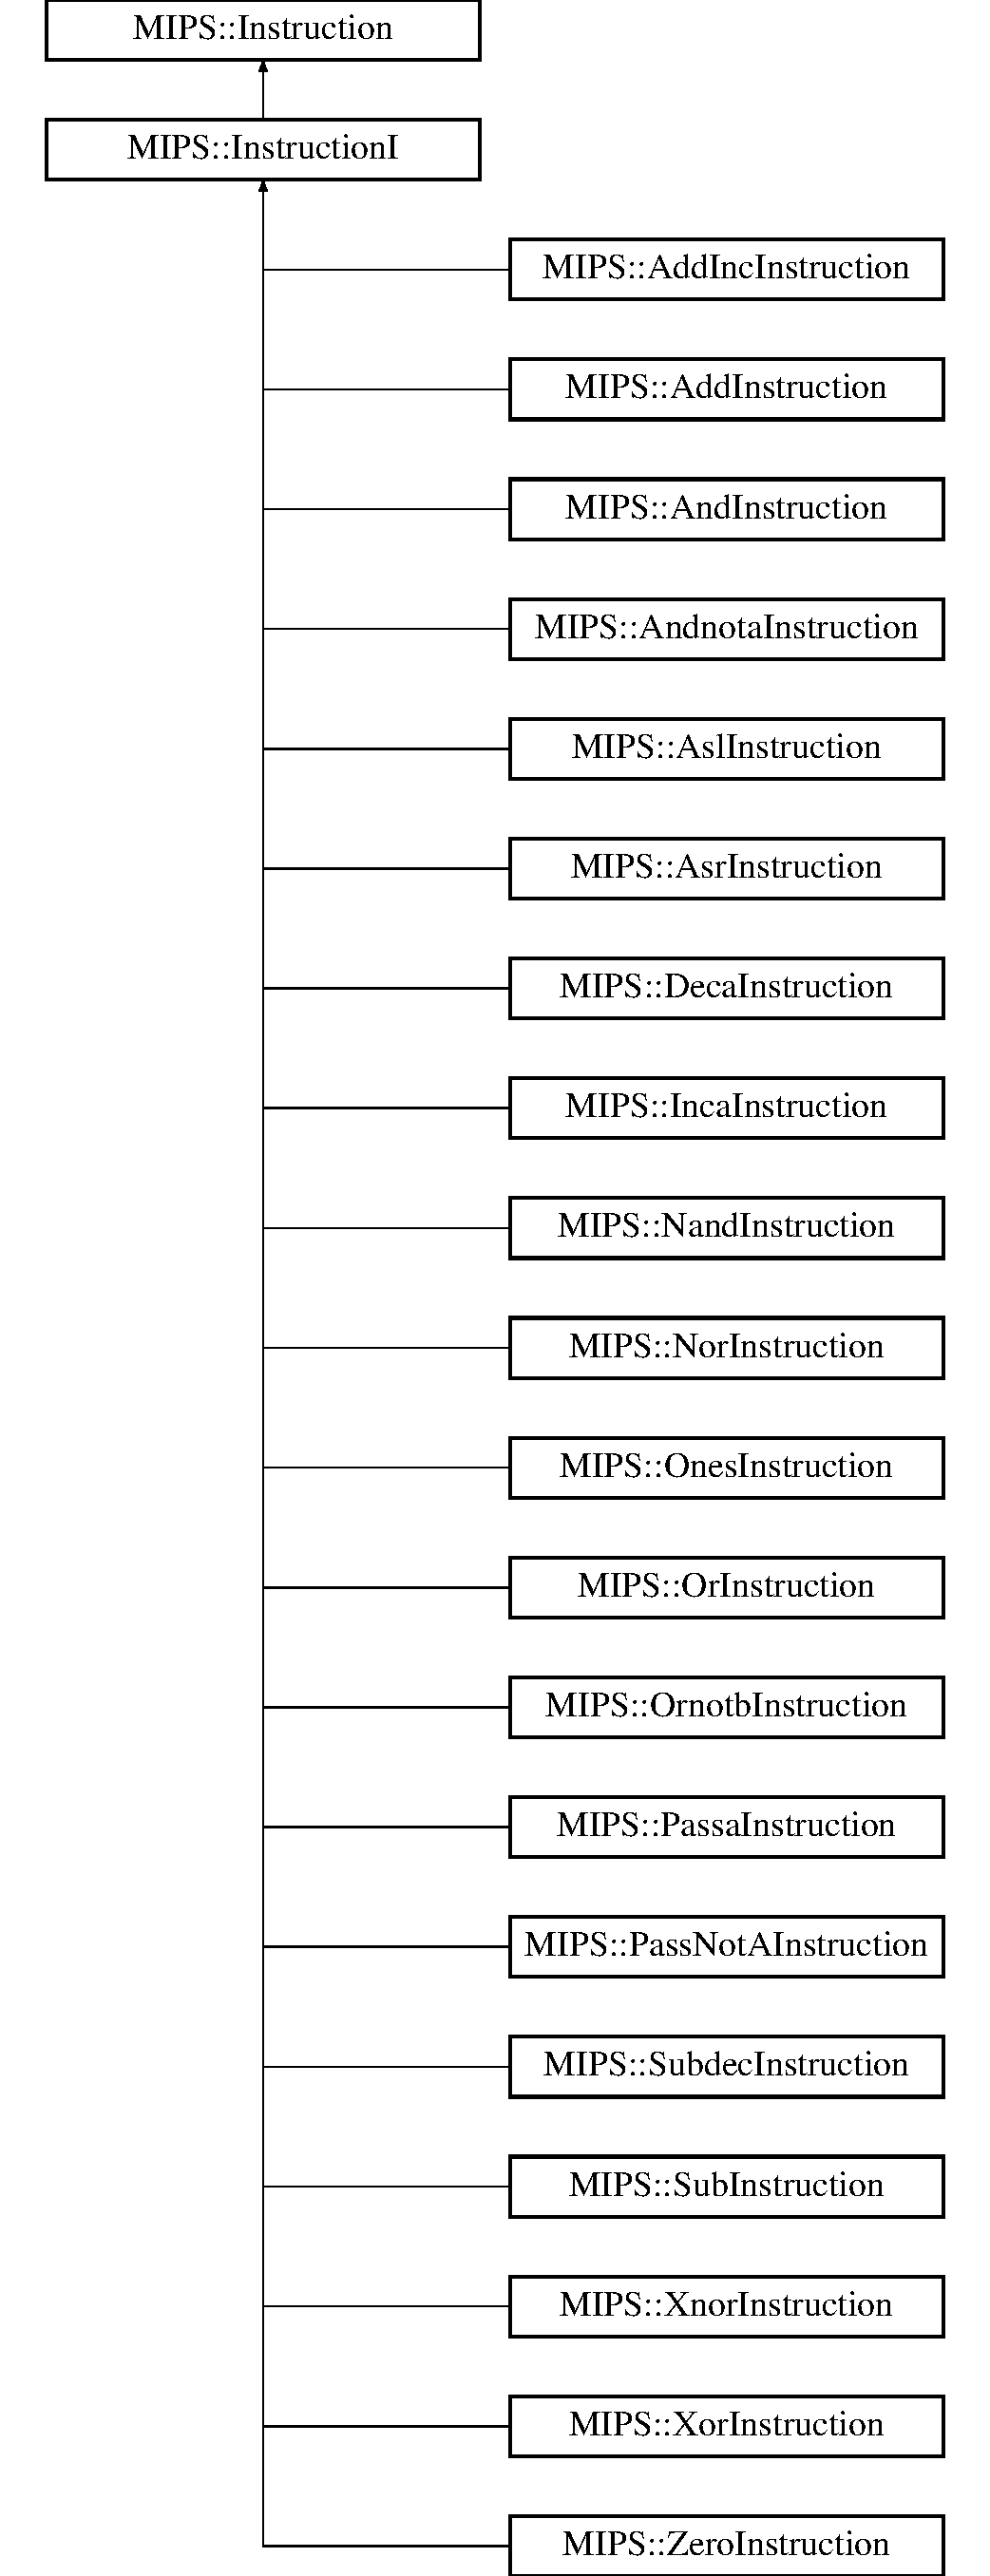
\includegraphics[height=12.000000cm]{classMIPS_1_1InstructionI}
\end{center}
\end{figure}
\subsection*{Public Member Functions}
\begin{DoxyCompactItemize}
\item 
\hyperlink{classMIPS_1_1InstructionI_a57bdbde86da12b395952eea141867ec2}{InstructionI} (\hyperlink{core_8hpp_a6074bae122ae7b527864eec42c728c3c}{bit8\+\_\+t} \hyperlink{classMIPS_1_1Instruction_a45cc6808b5dde8a5d41067d148b55476}{opcode}, \hyperlink{classMIPS_1_1Register}{Register} $\ast$\hyperlink{classMIPS_1_1InstructionI_a2be191d5b3dce505e2e626ec02eb4d62}{rs}, \hyperlink{classMIPS_1_1Register}{Register} $\ast$\hyperlink{classMIPS_1_1InstructionI_add1db07a5c954f35271de8c8a5737487}{rt}, \hyperlink{core_8hpp_a6074bae122ae7b527864eec42c728c3c}{bit8\+\_\+t} \hyperlink{classMIPS_1_1InstructionI_aa9b6da37c374c2ec8d96448d341e5e7d}{shamt}, \hyperlink{core_8hpp_a6074bae122ae7b527864eec42c728c3c}{bit8\+\_\+t} \hyperlink{classMIPS_1_1InstructionI_a5c6efcbbd233a7447c1fe24ea0a1e558}{funct})
\item 
virtual \hyperlink{classMIPS_1_1InstructionI_ae330e8a6a7d5820b0e559a7845867518}{$\sim$\+InstructionI} ()
\item 
virtual \hyperlink{core_8hpp_adc265a970bc35995b5879784bbb3f1b7}{bit16\+\_\+t} \hyperlink{classMIPS_1_1InstructionI_ae60fca5801bf5415cdff06d2aa11764f}{execute} ()=0
\end{DoxyCompactItemize}
\subsection*{Protected Attributes}
\begin{DoxyCompactItemize}
\item 
\hyperlink{classMIPS_1_1Register}{Register} $\ast$ \hyperlink{classMIPS_1_1InstructionI_a2be191d5b3dce505e2e626ec02eb4d62}{rs}
\item 
\hyperlink{classMIPS_1_1Register}{Register} $\ast$ \hyperlink{classMIPS_1_1InstructionI_add1db07a5c954f35271de8c8a5737487}{rt}
\item 
\hyperlink{core_8hpp_a6074bae122ae7b527864eec42c728c3c}{bit8\+\_\+t} \hyperlink{classMIPS_1_1InstructionI_aa9b6da37c374c2ec8d96448d341e5e7d}{shamt}
\item 
\hyperlink{core_8hpp_a6074bae122ae7b527864eec42c728c3c}{bit8\+\_\+t} \hyperlink{classMIPS_1_1InstructionI_a5c6efcbbd233a7447c1fe24ea0a1e558}{funct}
\end{DoxyCompactItemize}


\subsection{Detailed Description}
Classe que representa uma instrução do tipo (R)egister.

\begin{DoxyAuthor}{Author}
Matheus Nogueira 
\end{DoxyAuthor}


\subsection{Constructor \& Destructor Documentation}
\index{M\+I\+P\+S\+::\+InstructionI@{M\+I\+P\+S\+::\+InstructionI}!InstructionI@{InstructionI}}
\index{InstructionI@{InstructionI}!M\+I\+P\+S\+::\+InstructionI@{M\+I\+P\+S\+::\+InstructionI}}
\subsubsection[{\texorpdfstring{Instruction\+I(bit8\+\_\+t opcode, Register $\ast$rs, Register $\ast$rt, bit8\+\_\+t shamt, bit8\+\_\+t funct)}{InstructionI(bit8_t opcode, Register *rs, Register *rt, bit8_t shamt, bit8_t funct)}}]{\setlength{\rightskip}{0pt plus 5cm}M\+I\+P\+S\+::\+Instruction\+I\+::\+InstructionI (
\begin{DoxyParamCaption}
\item[{{\bf bit8\+\_\+t}}]{opcode, }
\item[{{\bf Register} $\ast$}]{rs, }
\item[{{\bf Register} $\ast$}]{rt, }
\item[{{\bf bit8\+\_\+t}}]{shamt, }
\item[{{\bf bit8\+\_\+t}}]{funct}
\end{DoxyParamCaption}
)\hspace{0.3cm}{\ttfamily [inline]}}\hypertarget{classMIPS_1_1InstructionI_a57bdbde86da12b395952eea141867ec2}{}\label{classMIPS_1_1InstructionI_a57bdbde86da12b395952eea141867ec2}
Cria uma nova instrução do formato I.


\begin{DoxyParams}{Parameters}
{\em opcode} & codigo da operação \\
\hline
{\em rs} & registrador source \\
\hline
{\em rt} & registrador target \\
\hline
{\em rd} & registrador destination \\
\hline
{\em shamt} & quantidade de shift \\
\hline
{\em funct} & bits para escolha da função da instrução \\
\hline
\end{DoxyParams}
\index{M\+I\+P\+S\+::\+InstructionI@{M\+I\+P\+S\+::\+InstructionI}!````~InstructionI@{$\sim$\+InstructionI}}
\index{````~InstructionI@{$\sim$\+InstructionI}!M\+I\+P\+S\+::\+InstructionI@{M\+I\+P\+S\+::\+InstructionI}}
\subsubsection[{\texorpdfstring{$\sim$\+Instruction\+I()}{~InstructionI()}}]{\setlength{\rightskip}{0pt plus 5cm}virtual M\+I\+P\+S\+::\+Instruction\+I\+::$\sim$\+InstructionI (
\begin{DoxyParamCaption}
{}
\end{DoxyParamCaption}
)\hspace{0.3cm}{\ttfamily [inline]}, {\ttfamily [virtual]}}\hypertarget{classMIPS_1_1InstructionI_ae330e8a6a7d5820b0e559a7845867518}{}\label{classMIPS_1_1InstructionI_ae330e8a6a7d5820b0e559a7845867518}
Destroi a instrução. 

\subsection{Member Function Documentation}
\index{M\+I\+P\+S\+::\+InstructionI@{M\+I\+P\+S\+::\+InstructionI}!execute@{execute}}
\index{execute@{execute}!M\+I\+P\+S\+::\+InstructionI@{M\+I\+P\+S\+::\+InstructionI}}
\subsubsection[{\texorpdfstring{execute()=0}{execute()=0}}]{\setlength{\rightskip}{0pt plus 5cm}virtual {\bf bit16\+\_\+t} M\+I\+P\+S\+::\+Instruction\+I\+::execute (
\begin{DoxyParamCaption}
{}
\end{DoxyParamCaption}
)\hspace{0.3cm}{\ttfamily [pure virtual]}}\hypertarget{classMIPS_1_1InstructionI_ae60fca5801bf5415cdff06d2aa11764f}{}\label{classMIPS_1_1InstructionI_ae60fca5801bf5415cdff06d2aa11764f}
Executa a instrução.

\begin{DoxyReturn}{Returns}
resultado da instrução 
\end{DoxyReturn}


Implements \hyperlink{classMIPS_1_1Instruction_a88668dfaf49dd8608f210ba13948d242}{M\+I\+P\+S\+::\+Instruction}.



Implemented in \hyperlink{classMIPS_1_1AddInstruction_aa699dc00fdcd4250944f8afaa2fa89eb}{M\+I\+P\+S\+::\+Add\+Instruction}, \hyperlink{classMIPS_1_1AddIncInstruction_aa63fcaf17a9afc2f1b5d09a6291a70d6}{M\+I\+P\+S\+::\+Add\+Inc\+Instruction}, \hyperlink{classMIPS_1_1AndnotaInstruction_afdc3b2836318f4adaa32dfa3bcdf7c45}{M\+I\+P\+S\+::\+Andnota\+Instruction}, \hyperlink{classMIPS_1_1AslInstruction_adafc2d1f549cda9bdf757dc2bac03ca9}{M\+I\+P\+S\+::\+Asl\+Instruction}, \hyperlink{classMIPS_1_1AsrInstruction_aad46283e10517abf6bf5e527ca020d53}{M\+I\+P\+S\+::\+Asr\+Instruction}, \hyperlink{classMIPS_1_1DecaInstruction_a82c3d685d910d2c52163f5faa1750aca}{M\+I\+P\+S\+::\+Deca\+Instruction}, \hyperlink{classMIPS_1_1IncaInstruction_ac78e4a0b037ab4b6b419f4f5a34413c7}{M\+I\+P\+S\+::\+Inca\+Instruction}, \hyperlink{classMIPS_1_1NandInstruction_a2e0266ebee3819e7b4d9bfb44f0e70ac}{M\+I\+P\+S\+::\+Nand\+Instruction}, \hyperlink{classMIPS_1_1NorInstruction_a68bb5cc9920bd63229f4c16c4edb5ab6}{M\+I\+P\+S\+::\+Nor\+Instruction}, \hyperlink{classMIPS_1_1OnesInstruction_aeab25fd32df5c092d4f426371f3f1ff3}{M\+I\+P\+S\+::\+Ones\+Instruction}, \hyperlink{classMIPS_1_1PassaInstruction_ae23b43bfb84d2ef69fa25e50fb5b6072}{M\+I\+P\+S\+::\+Passa\+Instruction}, \hyperlink{classMIPS_1_1PassNotAInstruction_a30b9bdb1feac1adb44e70a3a0eb85cb4}{M\+I\+P\+S\+::\+Pass\+Not\+A\+Instruction}, \hyperlink{classMIPS_1_1SubInstruction_a2b10f6bfda0e7d9651600b530cfccf62}{M\+I\+P\+S\+::\+Sub\+Instruction}, \hyperlink{classMIPS_1_1XnorInstruction_a4b5ae9a875883902c0ed1e237e753f31}{M\+I\+P\+S\+::\+Xnor\+Instruction}, \hyperlink{classMIPS_1_1XorInstruction_aaebc7dc8723627871ba2caf85f01fbea}{M\+I\+P\+S\+::\+Xor\+Instruction}, \hyperlink{classMIPS_1_1ZeroInstruction_a9596a96b4bf7a51672ab14386d111bad}{M\+I\+P\+S\+::\+Zero\+Instruction}, \hyperlink{classMIPS_1_1SubdecInstruction_a6d9e86774b950a584b60d9a48402af2a}{M\+I\+P\+S\+::\+Subdec\+Instruction}, \hyperlink{classMIPS_1_1AndInstruction_a24b2fdb68ff022275db4181e502b7a48}{M\+I\+P\+S\+::\+And\+Instruction}, \hyperlink{classMIPS_1_1OrInstruction_a89859e0bcb3e5ed7f1c53f33f627f041}{M\+I\+P\+S\+::\+Or\+Instruction}, and \hyperlink{classMIPS_1_1OrnotbInstruction_a47aac4ac3ef0ee8c6a694189f26bd80e}{M\+I\+P\+S\+::\+Ornotb\+Instruction}.



\subsection{Member Data Documentation}
\index{M\+I\+P\+S\+::\+InstructionI@{M\+I\+P\+S\+::\+InstructionI}!funct@{funct}}
\index{funct@{funct}!M\+I\+P\+S\+::\+InstructionI@{M\+I\+P\+S\+::\+InstructionI}}
\subsubsection[{\texorpdfstring{funct}{funct}}]{\setlength{\rightskip}{0pt plus 5cm}{\bf bit8\+\_\+t} M\+I\+P\+S\+::\+Instruction\+I\+::funct\hspace{0.3cm}{\ttfamily [protected]}}\hypertarget{classMIPS_1_1InstructionI_a5c6efcbbd233a7447c1fe24ea0a1e558}{}\label{classMIPS_1_1InstructionI_a5c6efcbbd233a7447c1fe24ea0a1e558}
Valor da funct da instrução. \index{M\+I\+P\+S\+::\+InstructionI@{M\+I\+P\+S\+::\+InstructionI}!rs@{rs}}
\index{rs@{rs}!M\+I\+P\+S\+::\+InstructionI@{M\+I\+P\+S\+::\+InstructionI}}
\subsubsection[{\texorpdfstring{rs}{rs}}]{\setlength{\rightskip}{0pt plus 5cm}{\bf Register}$\ast$ M\+I\+P\+S\+::\+Instruction\+I\+::rs\hspace{0.3cm}{\ttfamily [protected]}}\hypertarget{classMIPS_1_1InstructionI_a2be191d5b3dce505e2e626ec02eb4d62}{}\label{classMIPS_1_1InstructionI_a2be191d5b3dce505e2e626ec02eb4d62}
Registrador source (Rs) da instrução. \index{M\+I\+P\+S\+::\+InstructionI@{M\+I\+P\+S\+::\+InstructionI}!rt@{rt}}
\index{rt@{rt}!M\+I\+P\+S\+::\+InstructionI@{M\+I\+P\+S\+::\+InstructionI}}
\subsubsection[{\texorpdfstring{rt}{rt}}]{\setlength{\rightskip}{0pt plus 5cm}{\bf Register}$\ast$ M\+I\+P\+S\+::\+Instruction\+I\+::rt\hspace{0.3cm}{\ttfamily [protected]}}\hypertarget{classMIPS_1_1InstructionI_add1db07a5c954f35271de8c8a5737487}{}\label{classMIPS_1_1InstructionI_add1db07a5c954f35271de8c8a5737487}
Registrador target (Rt) da instrução. \index{M\+I\+P\+S\+::\+InstructionI@{M\+I\+P\+S\+::\+InstructionI}!shamt@{shamt}}
\index{shamt@{shamt}!M\+I\+P\+S\+::\+InstructionI@{M\+I\+P\+S\+::\+InstructionI}}
\subsubsection[{\texorpdfstring{shamt}{shamt}}]{\setlength{\rightskip}{0pt plus 5cm}{\bf bit8\+\_\+t} M\+I\+P\+S\+::\+Instruction\+I\+::shamt\hspace{0.3cm}{\ttfamily [protected]}}\hypertarget{classMIPS_1_1InstructionI_aa9b6da37c374c2ec8d96448d341e5e7d}{}\label{classMIPS_1_1InstructionI_aa9b6da37c374c2ec8d96448d341e5e7d}
Valor do shamt (shift amount) da instrução. 

The documentation for this class was generated from the following file\+:\begin{DoxyCompactItemize}
\item 
include/mips/instructions/\hyperlink{instruction__I_8hpp}{instruction\+\_\+\+I.\+hpp}\end{DoxyCompactItemize}

\hypertarget{classMIPS_1_1InstructionII}{}\section{M\+I\+PS\+:\+:Instruction\+II Class Reference}
\label{classMIPS_1_1InstructionII}\index{M\+I\+P\+S\+::\+Instruction\+II@{M\+I\+P\+S\+::\+Instruction\+II}}


{\ttfamily \#include $<$instruction\+\_\+\+I\+I.\+hpp$>$}

Inheritance diagram for M\+I\+PS\+:\+:Instruction\+II\+:\begin{figure}[H]
\begin{center}
\leavevmode
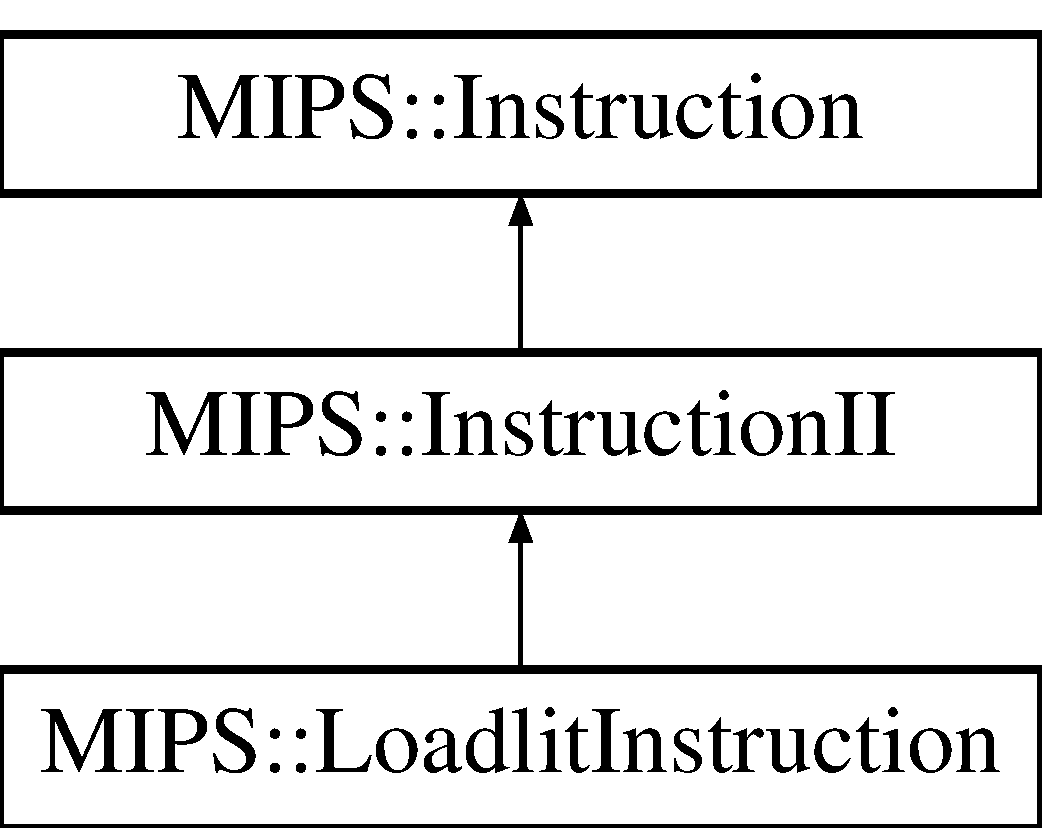
\includegraphics[height=3.000000cm]{classMIPS_1_1InstructionII}
\end{center}
\end{figure}
\subsection*{Public Member Functions}
\begin{DoxyCompactItemize}
\item 
\hyperlink{classMIPS_1_1InstructionII_a0f84efe08b176134df068fed51aca447}{Instruction\+II} (\hyperlink{core_8hpp_a6074bae122ae7b527864eec42c728c3c}{bit8\+\_\+t} \hyperlink{classMIPS_1_1Instruction_a45cc6808b5dde8a5d41067d148b55476}{opcode}, \hyperlink{classMIPS_1_1Register}{Register} $\ast$\hyperlink{classMIPS_1_1InstructionII_a2a709b8170f2bf653de2102df9403e1f}{rd}, \hyperlink{core_8hpp_adc265a970bc35995b5879784bbb3f1b7}{bit16\+\_\+t} \hyperlink{classMIPS_1_1InstructionII_ae34cdcf18cd37944dfecb96d5b07b5cb}{offset})
\item 
virtual \hyperlink{core_8hpp_adc265a970bc35995b5879784bbb3f1b7}{bit16\+\_\+t} \hyperlink{classMIPS_1_1InstructionII_aa014c5b0fe877746ca4db85c971a2e93}{execute} ()=0
\end{DoxyCompactItemize}
\subsection*{Protected Attributes}
\begin{DoxyCompactItemize}
\item 
\hyperlink{classMIPS_1_1Register}{Register} $\ast$ \hyperlink{classMIPS_1_1InstructionII_a2a709b8170f2bf653de2102df9403e1f}{rd}
\item 
\hyperlink{core_8hpp_adc265a970bc35995b5879784bbb3f1b7}{bit16\+\_\+t} \hyperlink{classMIPS_1_1InstructionII_ae34cdcf18cd37944dfecb96d5b07b5cb}{offset}
\end{DoxyCompactItemize}


\subsection{Detailed Description}
Classe que representa uma instrução do formato II do trabalho.

\begin{DoxyAuthor}{Author}
Matheus Nogueira 
\end{DoxyAuthor}


\subsection{Constructor \& Destructor Documentation}
\index{M\+I\+P\+S\+::\+Instruction\+II@{M\+I\+P\+S\+::\+Instruction\+II}!Instruction\+II@{Instruction\+II}}
\index{Instruction\+II@{Instruction\+II}!M\+I\+P\+S\+::\+Instruction\+II@{M\+I\+P\+S\+::\+Instruction\+II}}
\subsubsection[{\texorpdfstring{Instruction\+I\+I(bit8\+\_\+t opcode, Register $\ast$rd, bit16\+\_\+t offset)}{InstructionII(bit8_t opcode, Register *rd, bit16_t offset)}}]{\setlength{\rightskip}{0pt plus 5cm}M\+I\+P\+S\+::\+Instruction\+I\+I\+::\+Instruction\+II (
\begin{DoxyParamCaption}
\item[{{\bf bit8\+\_\+t}}]{opcode, }
\item[{{\bf Register} $\ast$}]{rd, }
\item[{{\bf bit16\+\_\+t}}]{offset}
\end{DoxyParamCaption}
)\hspace{0.3cm}{\ttfamily [inline]}}\hypertarget{classMIPS_1_1InstructionII_a0f84efe08b176134df068fed51aca447}{}\label{classMIPS_1_1InstructionII_a0f84efe08b176134df068fed51aca447}
Cria uma nova instrução do formato II


\begin{DoxyParams}{Parameters}
{\em opcode} & código da operação \\
\hline
{\em rd} & registrador de destino \\
\hline
{\em offset} & offset de 11 bits. \\
\hline
\end{DoxyParams}


\subsection{Member Function Documentation}
\index{M\+I\+P\+S\+::\+Instruction\+II@{M\+I\+P\+S\+::\+Instruction\+II}!execute@{execute}}
\index{execute@{execute}!M\+I\+P\+S\+::\+Instruction\+II@{M\+I\+P\+S\+::\+Instruction\+II}}
\subsubsection[{\texorpdfstring{execute()=0}{execute()=0}}]{\setlength{\rightskip}{0pt plus 5cm}virtual {\bf bit16\+\_\+t} M\+I\+P\+S\+::\+Instruction\+I\+I\+::execute (
\begin{DoxyParamCaption}
{}
\end{DoxyParamCaption}
)\hspace{0.3cm}{\ttfamily [pure virtual]}}\hypertarget{classMIPS_1_1InstructionII_aa014c5b0fe877746ca4db85c971a2e93}{}\label{classMIPS_1_1InstructionII_aa014c5b0fe877746ca4db85c971a2e93}
Executa a instrução.

\begin{DoxyReturn}{Returns}
resultado da instrução 
\end{DoxyReturn}


Implements \hyperlink{classMIPS_1_1Instruction_a88668dfaf49dd8608f210ba13948d242}{M\+I\+P\+S\+::\+Instruction}.



Implemented in \hyperlink{classMIPS_1_1LoadlitInstruction_a9f88a932bbbf31375da7686b449608e1}{M\+I\+P\+S\+::\+Loadlit\+Instruction}.



\subsection{Member Data Documentation}
\index{M\+I\+P\+S\+::\+Instruction\+II@{M\+I\+P\+S\+::\+Instruction\+II}!offset@{offset}}
\index{offset@{offset}!M\+I\+P\+S\+::\+Instruction\+II@{M\+I\+P\+S\+::\+Instruction\+II}}
\subsubsection[{\texorpdfstring{offset}{offset}}]{\setlength{\rightskip}{0pt plus 5cm}{\bf bit16\+\_\+t} M\+I\+P\+S\+::\+Instruction\+I\+I\+::offset\hspace{0.3cm}{\ttfamily [protected]}}\hypertarget{classMIPS_1_1InstructionII_ae34cdcf18cd37944dfecb96d5b07b5cb}{}\label{classMIPS_1_1InstructionII_ae34cdcf18cd37944dfecb96d5b07b5cb}
Offset utilizado pela instrução. \index{M\+I\+P\+S\+::\+Instruction\+II@{M\+I\+P\+S\+::\+Instruction\+II}!rd@{rd}}
\index{rd@{rd}!M\+I\+P\+S\+::\+Instruction\+II@{M\+I\+P\+S\+::\+Instruction\+II}}
\subsubsection[{\texorpdfstring{rd}{rd}}]{\setlength{\rightskip}{0pt plus 5cm}{\bf Register}$\ast$ M\+I\+P\+S\+::\+Instruction\+I\+I\+::rd\hspace{0.3cm}{\ttfamily [protected]}}\hypertarget{classMIPS_1_1InstructionII_a2a709b8170f2bf653de2102df9403e1f}{}\label{classMIPS_1_1InstructionII_a2a709b8170f2bf653de2102df9403e1f}
Registrador de destino da instrução. 

The documentation for this class was generated from the following file\+:\begin{DoxyCompactItemize}
\item 
include/mips/instructions/\hyperlink{instruction__II_8hpp}{instruction\+\_\+\+I\+I.\+hpp}\end{DoxyCompactItemize}

\hypertarget{classMIPS_1_1InstructionIII}{}\section{M\+I\+PS\+:\+:Instruction\+I\+II Class Reference}
\label{classMIPS_1_1InstructionIII}\index{M\+I\+P\+S\+::\+Instruction\+I\+II@{M\+I\+P\+S\+::\+Instruction\+I\+II}}


{\ttfamily \#include $<$instruction\+\_\+\+I\+I\+I.\+hpp$>$}

Inheritance diagram for M\+I\+PS\+:\+:Instruction\+I\+II\+:\begin{figure}[H]
\begin{center}
\leavevmode
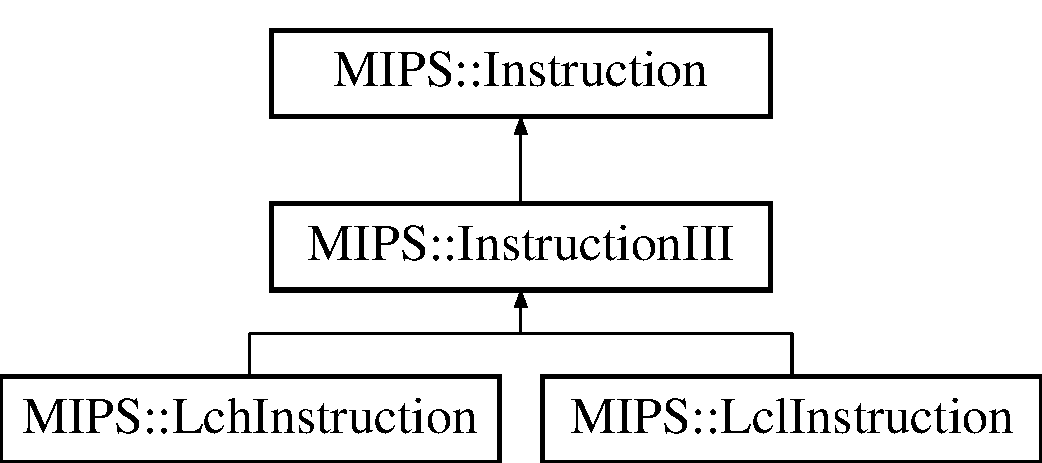
\includegraphics[height=3.000000cm]{classMIPS_1_1InstructionIII}
\end{center}
\end{figure}
\subsection*{Public Member Functions}
\begin{DoxyCompactItemize}
\item 
\hyperlink{classMIPS_1_1InstructionIII_a0b3a67569e09bd53866536d5241a3d17}{Instruction\+I\+II} (\hyperlink{core_8hpp_a6074bae122ae7b527864eec42c728c3c}{bit8\+\_\+t} \hyperlink{classMIPS_1_1Instruction_a45cc6808b5dde8a5d41067d148b55476}{opcode}, \hyperlink{classMIPS_1_1Register}{Register} $\ast$\hyperlink{classMIPS_1_1InstructionIII_a76e7b218fc57cd2fc559bf72498090b6}{rd}, \hyperlink{core_8hpp_a6074bae122ae7b527864eec42c728c3c}{bit8\+\_\+t} \hyperlink{classMIPS_1_1InstructionIII_ad0ebd3b6e7594fc583e9a409bf99a6c7}{offset})
\item 
virtual \hyperlink{core_8hpp_adc265a970bc35995b5879784bbb3f1b7}{bit16\+\_\+t} \hyperlink{classMIPS_1_1InstructionIII_aee3071c23abc542e55b446abee766c5e}{execute} ()=0
\item 
void \hyperlink{classMIPS_1_1InstructionIII_ac2e82988e8b0b356f939d86c3de5ed59}{update\+Control} (\hyperlink{classMIPS_1_1ControlUnit}{Control\+Unit} \&control)
\end{DoxyCompactItemize}
\subsection*{Protected Attributes}
\begin{DoxyCompactItemize}
\item 
\hyperlink{classMIPS_1_1Register}{Register} $\ast$ \hyperlink{classMIPS_1_1InstructionIII_a76e7b218fc57cd2fc559bf72498090b6}{rd}
\item 
\hyperlink{core_8hpp_a6074bae122ae7b527864eec42c728c3c}{bit8\+\_\+t} \hyperlink{classMIPS_1_1InstructionIII_ad0ebd3b6e7594fc583e9a409bf99a6c7}{offset}
\end{DoxyCompactItemize}


\subsection{Detailed Description}
Classe que representa uma instrução do formato I\+II do trabalho.

\begin{DoxyAuthor}{Author}
Matheus Nogueira 
\end{DoxyAuthor}


\subsection{Constructor \& Destructor Documentation}
\index{M\+I\+P\+S\+::\+Instruction\+I\+II@{M\+I\+P\+S\+::\+Instruction\+I\+II}!Instruction\+I\+II@{Instruction\+I\+II}}
\index{Instruction\+I\+II@{Instruction\+I\+II}!M\+I\+P\+S\+::\+Instruction\+I\+II@{M\+I\+P\+S\+::\+Instruction\+I\+II}}
\subsubsection[{\texorpdfstring{Instruction\+I\+I\+I(bit8\+\_\+t opcode, Register $\ast$rd, bit8\+\_\+t offset)}{InstructionIII(bit8_t opcode, Register *rd, bit8_t offset)}}]{\setlength{\rightskip}{0pt plus 5cm}M\+I\+P\+S\+::\+Instruction\+I\+I\+I\+::\+Instruction\+I\+II (
\begin{DoxyParamCaption}
\item[{{\bf bit8\+\_\+t}}]{opcode, }
\item[{{\bf Register} $\ast$}]{rd, }
\item[{{\bf bit8\+\_\+t}}]{offset}
\end{DoxyParamCaption}
)\hspace{0.3cm}{\ttfamily [inline]}}\hypertarget{classMIPS_1_1InstructionIII_a0b3a67569e09bd53866536d5241a3d17}{}\label{classMIPS_1_1InstructionIII_a0b3a67569e09bd53866536d5241a3d17}
Cria uma nova instrução do formato I\+II


\begin{DoxyParams}{Parameters}
{\em opcode} & código da operação \\
\hline
{\em rd} & registrador de destino \\
\hline
{\em offset} & offset de 8 bits \\
\hline
\end{DoxyParams}


\subsection{Member Function Documentation}
\index{M\+I\+P\+S\+::\+Instruction\+I\+II@{M\+I\+P\+S\+::\+Instruction\+I\+II}!execute@{execute}}
\index{execute@{execute}!M\+I\+P\+S\+::\+Instruction\+I\+II@{M\+I\+P\+S\+::\+Instruction\+I\+II}}
\subsubsection[{\texorpdfstring{execute()=0}{execute()=0}}]{\setlength{\rightskip}{0pt plus 5cm}virtual {\bf bit16\+\_\+t} M\+I\+P\+S\+::\+Instruction\+I\+I\+I\+::execute (
\begin{DoxyParamCaption}
{}
\end{DoxyParamCaption}
)\hspace{0.3cm}{\ttfamily [pure virtual]}}\hypertarget{classMIPS_1_1InstructionIII_aee3071c23abc542e55b446abee766c5e}{}\label{classMIPS_1_1InstructionIII_aee3071c23abc542e55b446abee766c5e}
Executa a instrução.

\begin{DoxyReturn}{Returns}
resultado da instrução 
\end{DoxyReturn}


Implements \hyperlink{classMIPS_1_1Instruction_a88668dfaf49dd8608f210ba13948d242}{M\+I\+P\+S\+::\+Instruction}.



Implemented in \hyperlink{classMIPS_1_1LchInstruction_a6dad60c9189a1e84fd7c789b9642077d}{M\+I\+P\+S\+::\+Lch\+Instruction}, and \hyperlink{classMIPS_1_1LclInstruction_a713c7c0e33c9df49f677abfd95f363db}{M\+I\+P\+S\+::\+Lcl\+Instruction}.

\index{M\+I\+P\+S\+::\+Instruction\+I\+II@{M\+I\+P\+S\+::\+Instruction\+I\+II}!update\+Control@{update\+Control}}
\index{update\+Control@{update\+Control}!M\+I\+P\+S\+::\+Instruction\+I\+II@{M\+I\+P\+S\+::\+Instruction\+I\+II}}
\subsubsection[{\texorpdfstring{update\+Control(\+Control\+Unit \&control)}{updateControl(ControlUnit &control)}}]{\setlength{\rightskip}{0pt plus 5cm}void M\+I\+P\+S\+::\+Instruction\+I\+I\+I\+::update\+Control (
\begin{DoxyParamCaption}
\item[{{\bf Control\+Unit} \&}]{control}
\end{DoxyParamCaption}
)\hspace{0.3cm}{\ttfamily [inline]}, {\ttfamily [virtual]}}\hypertarget{classMIPS_1_1InstructionIII_ac2e82988e8b0b356f939d86c3de5ed59}{}\label{classMIPS_1_1InstructionIII_ac2e82988e8b0b356f939d86c3de5ed59}
Método utilizado para atualizar os sinais de controle do processador.


\begin{DoxyParams}{Parameters}
{\em control} & unidade de controle do processador. \\
\hline
\end{DoxyParams}


Reimplemented from \hyperlink{classMIPS_1_1Instruction_a7df847adef2997446ffca9b71c2f3112}{M\+I\+P\+S\+::\+Instruction}.



\subsection{Member Data Documentation}
\index{M\+I\+P\+S\+::\+Instruction\+I\+II@{M\+I\+P\+S\+::\+Instruction\+I\+II}!offset@{offset}}
\index{offset@{offset}!M\+I\+P\+S\+::\+Instruction\+I\+II@{M\+I\+P\+S\+::\+Instruction\+I\+II}}
\subsubsection[{\texorpdfstring{offset}{offset}}]{\setlength{\rightskip}{0pt plus 5cm}{\bf bit8\+\_\+t} M\+I\+P\+S\+::\+Instruction\+I\+I\+I\+::offset\hspace{0.3cm}{\ttfamily [protected]}}\hypertarget{classMIPS_1_1InstructionIII_ad0ebd3b6e7594fc583e9a409bf99a6c7}{}\label{classMIPS_1_1InstructionIII_ad0ebd3b6e7594fc583e9a409bf99a6c7}
Offset utilizado pela instrução. \index{M\+I\+P\+S\+::\+Instruction\+I\+II@{M\+I\+P\+S\+::\+Instruction\+I\+II}!rd@{rd}}
\index{rd@{rd}!M\+I\+P\+S\+::\+Instruction\+I\+II@{M\+I\+P\+S\+::\+Instruction\+I\+II}}
\subsubsection[{\texorpdfstring{rd}{rd}}]{\setlength{\rightskip}{0pt plus 5cm}{\bf Register}$\ast$ M\+I\+P\+S\+::\+Instruction\+I\+I\+I\+::rd\hspace{0.3cm}{\ttfamily [protected]}}\hypertarget{classMIPS_1_1InstructionIII_a76e7b218fc57cd2fc559bf72498090b6}{}\label{classMIPS_1_1InstructionIII_a76e7b218fc57cd2fc559bf72498090b6}
Registrador de destino da instrução. 

The documentation for this class was generated from the following file\+:\begin{DoxyCompactItemize}
\item 
include/mips/instructions/\hyperlink{instruction__III_8hpp}{instruction\+\_\+\+I\+I\+I.\+hpp}\end{DoxyCompactItemize}

\hypertarget{classMIPS_1_1InstructionIV}{}\section{M\+I\+PS\+:\+:Instruction\+IV Class Reference}
\label{classMIPS_1_1InstructionIV}\index{M\+I\+P\+S\+::\+Instruction\+IV@{M\+I\+P\+S\+::\+Instruction\+IV}}


{\ttfamily \#include $<$instruction\+\_\+\+I\+V.\+hpp$>$}

Inheritance diagram for M\+I\+PS\+:\+:Instruction\+IV\+:\begin{figure}[H]
\begin{center}
\leavevmode
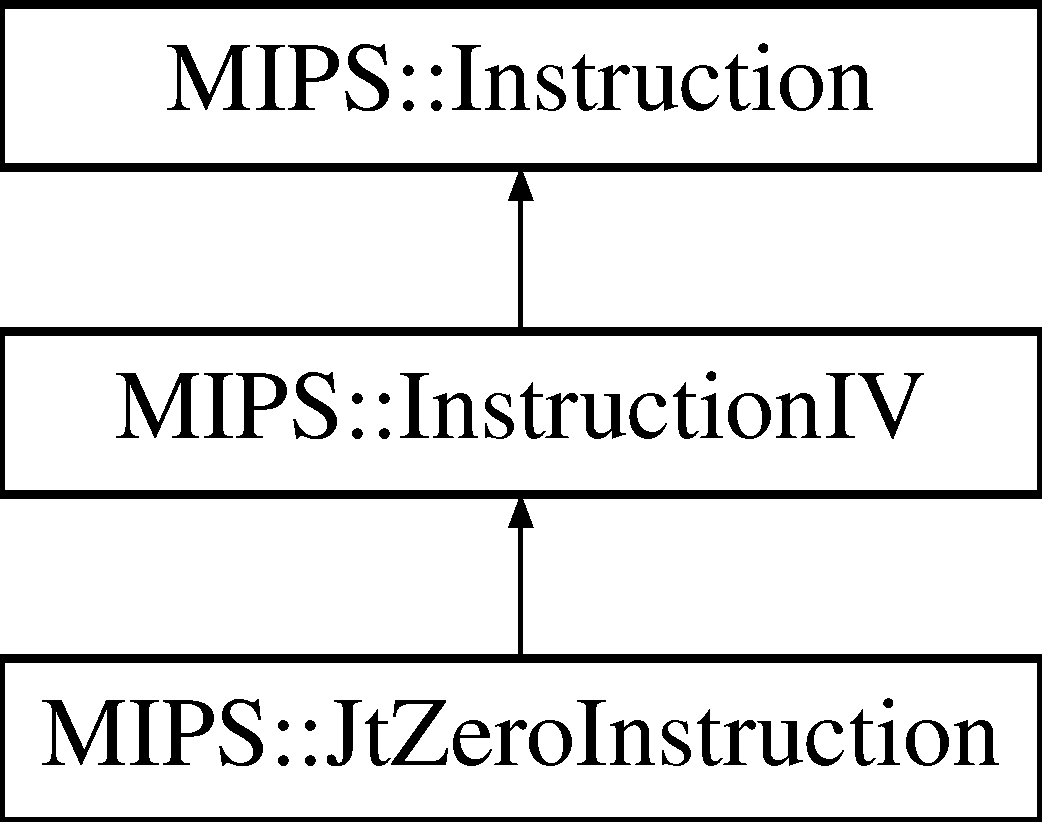
\includegraphics[height=3.000000cm]{classMIPS_1_1InstructionIV}
\end{center}
\end{figure}
\subsection*{Public Member Functions}
\begin{DoxyCompactItemize}
\item 
\hyperlink{classMIPS_1_1InstructionIV_a9219778a142dd2f6114ecf39bf9d24f3}{Instruction\+IV} (\hyperlink{core_8hpp_a6074bae122ae7b527864eec42c728c3c}{bit8\+\_\+t} \hyperlink{classMIPS_1_1Instruction_a45cc6808b5dde8a5d41067d148b55476}{opcode}, struct \hyperlink{structMIPS_1_1ALUFlags}{A\+L\+U\+Flags} \&alu\+Flags, \hyperlink{core_8hpp_a6074bae122ae7b527864eec42c728c3c}{bit8\+\_\+t} \hyperlink{classMIPS_1_1InstructionIV_abcb91e65c800a41bf9c46b5770120b36}{offset})
\item 
virtual \hyperlink{core_8hpp_adc265a970bc35995b5879784bbb3f1b7}{bit16\+\_\+t} \hyperlink{classMIPS_1_1InstructionIV_ae9eeb2c1aa5392cc3e2d9f2d816b799c}{execute} ()=0
\end{DoxyCompactItemize}
\subsection*{Protected Attributes}
\begin{DoxyCompactItemize}
\item 
\hyperlink{core_8hpp_a6074bae122ae7b527864eec42c728c3c}{bit8\+\_\+t} \hyperlink{classMIPS_1_1InstructionIV_abcb91e65c800a41bf9c46b5770120b36}{offset}
\item 
struct \hyperlink{structMIPS_1_1ALUFlags}{A\+L\+U\+Flags} \& \hyperlink{classMIPS_1_1InstructionIV_a7858449be2ee97f8ed852f7b8e8b4879}{flags}
\end{DoxyCompactItemize}


\subsection{Detailed Description}
Classe que representa uma instrução do formato IV do trabalho.

\begin{DoxyAuthor}{Author}
Matheus Nogueira 
\end{DoxyAuthor}


\subsection{Constructor \& Destructor Documentation}
\index{M\+I\+P\+S\+::\+Instruction\+IV@{M\+I\+P\+S\+::\+Instruction\+IV}!Instruction\+IV@{Instruction\+IV}}
\index{Instruction\+IV@{Instruction\+IV}!M\+I\+P\+S\+::\+Instruction\+IV@{M\+I\+P\+S\+::\+Instruction\+IV}}
\subsubsection[{\texorpdfstring{Instruction\+I\+V(bit8\+\_\+t opcode, struct A\+L\+U\+Flags \&alu\+Flags, bit8\+\_\+t offset)}{InstructionIV(bit8_t opcode, struct ALUFlags &aluFlags, bit8_t offset)}}]{\setlength{\rightskip}{0pt plus 5cm}M\+I\+P\+S\+::\+Instruction\+I\+V\+::\+Instruction\+IV (
\begin{DoxyParamCaption}
\item[{{\bf bit8\+\_\+t}}]{opcode, }
\item[{struct {\bf A\+L\+U\+Flags} \&}]{alu\+Flags, }
\item[{{\bf bit8\+\_\+t}}]{offset}
\end{DoxyParamCaption}
)\hspace{0.3cm}{\ttfamily [inline]}}\hypertarget{classMIPS_1_1InstructionIV_a9219778a142dd2f6114ecf39bf9d24f3}{}\label{classMIPS_1_1InstructionIV_a9219778a142dd2f6114ecf39bf9d24f3}
Cria uma nova instrução do formato IV


\begin{DoxyParams}{Parameters}
{\em opcode} & código da operação \\
\hline
{\em alu\+Flags} & Flags vindas da A\+LU \\
\hline
{\em offset} & offset do jump. \\
\hline
\end{DoxyParams}


\subsection{Member Function Documentation}
\index{M\+I\+P\+S\+::\+Instruction\+IV@{M\+I\+P\+S\+::\+Instruction\+IV}!execute@{execute}}
\index{execute@{execute}!M\+I\+P\+S\+::\+Instruction\+IV@{M\+I\+P\+S\+::\+Instruction\+IV}}
\subsubsection[{\texorpdfstring{execute()=0}{execute()=0}}]{\setlength{\rightskip}{0pt plus 5cm}virtual {\bf bit16\+\_\+t} M\+I\+P\+S\+::\+Instruction\+I\+V\+::execute (
\begin{DoxyParamCaption}
{}
\end{DoxyParamCaption}
)\hspace{0.3cm}{\ttfamily [pure virtual]}}\hypertarget{classMIPS_1_1InstructionIV_ae9eeb2c1aa5392cc3e2d9f2d816b799c}{}\label{classMIPS_1_1InstructionIV_ae9eeb2c1aa5392cc3e2d9f2d816b799c}
Executa a instrução.

\begin{DoxyReturn}{Returns}
0 se o desvio não é tomado, 1 se o desvio for tomado. 
\end{DoxyReturn}


Implements \hyperlink{classMIPS_1_1Instruction_a88668dfaf49dd8608f210ba13948d242}{M\+I\+P\+S\+::\+Instruction}.



Implemented in \hyperlink{classMIPS_1_1JtZeroInstruction_a8a56439dd5df5fcf00344304b8409e45}{M\+I\+P\+S\+::\+Jt\+Zero\+Instruction}.



\subsection{Member Data Documentation}
\index{M\+I\+P\+S\+::\+Instruction\+IV@{M\+I\+P\+S\+::\+Instruction\+IV}!flags@{flags}}
\index{flags@{flags}!M\+I\+P\+S\+::\+Instruction\+IV@{M\+I\+P\+S\+::\+Instruction\+IV}}
\subsubsection[{\texorpdfstring{flags}{flags}}]{\setlength{\rightskip}{0pt plus 5cm}struct {\bf A\+L\+U\+Flags}\& M\+I\+P\+S\+::\+Instruction\+I\+V\+::flags\hspace{0.3cm}{\ttfamily [protected]}}\hypertarget{classMIPS_1_1InstructionIV_a7858449be2ee97f8ed852f7b8e8b4879}{}\label{classMIPS_1_1InstructionIV_a7858449be2ee97f8ed852f7b8e8b4879}
Flags de saída da A\+LU \index{M\+I\+P\+S\+::\+Instruction\+IV@{M\+I\+P\+S\+::\+Instruction\+IV}!offset@{offset}}
\index{offset@{offset}!M\+I\+P\+S\+::\+Instruction\+IV@{M\+I\+P\+S\+::\+Instruction\+IV}}
\subsubsection[{\texorpdfstring{offset}{offset}}]{\setlength{\rightskip}{0pt plus 5cm}{\bf bit8\+\_\+t} M\+I\+P\+S\+::\+Instruction\+I\+V\+::offset\hspace{0.3cm}{\ttfamily [protected]}}\hypertarget{classMIPS_1_1InstructionIV_abcb91e65c800a41bf9c46b5770120b36}{}\label{classMIPS_1_1InstructionIV_abcb91e65c800a41bf9c46b5770120b36}
Offset da instrução de jump 

The documentation for this class was generated from the following file\+:\begin{DoxyCompactItemize}
\item 
include/mips/instructions/\hyperlink{instruction__IV_8hpp}{instruction\+\_\+\+I\+V.\+hpp}\end{DoxyCompactItemize}

\hypertarget{classMIPS_1_1InstructionV}{}\section{M\+I\+PS\+:\+:InstructionV Class Reference}
\label{classMIPS_1_1InstructionV}\index{M\+I\+P\+S\+::\+InstructionV@{M\+I\+P\+S\+::\+InstructionV}}


{\ttfamily \#include $<$instruction\+\_\+\+V.\+hpp$>$}

Inheritance diagram for M\+I\+PS\+:\+:InstructionV\+:\begin{figure}[H]
\begin{center}
\leavevmode
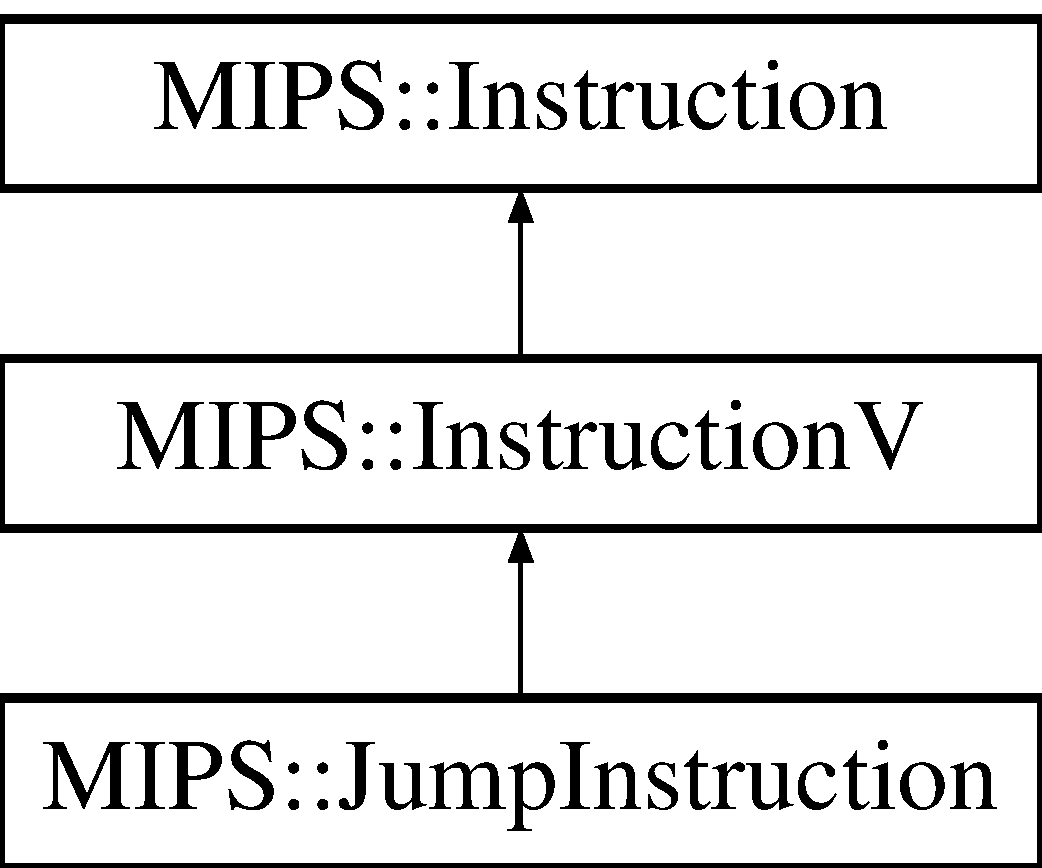
\includegraphics[height=3.000000cm]{classMIPS_1_1InstructionV}
\end{center}
\end{figure}
\subsection*{Public Member Functions}
\begin{DoxyCompactItemize}
\item 
\hyperlink{classMIPS_1_1InstructionV_a258d90fae989725cbada7cd80a626d73}{InstructionV} (\hyperlink{core_8hpp_a6074bae122ae7b527864eec42c728c3c}{bit8\+\_\+t} \hyperlink{classMIPS_1_1Instruction_a45cc6808b5dde8a5d41067d148b55476}{opcode}, \hyperlink{core_8hpp_adc265a970bc35995b5879784bbb3f1b7}{bit16\+\_\+t} \hyperlink{classMIPS_1_1InstructionV_ac2e294fde4971aa6a149480f22ae29e9}{offset})
\item 
virtual \hyperlink{core_8hpp_adc265a970bc35995b5879784bbb3f1b7}{bit16\+\_\+t} \hyperlink{classMIPS_1_1InstructionV_a511d8ba098bcca95f1e91ff6616470ef}{execute} ()=0
\end{DoxyCompactItemize}
\subsection*{Protected Attributes}
\begin{DoxyCompactItemize}
\item 
\hyperlink{core_8hpp_adc265a970bc35995b5879784bbb3f1b7}{bit16\+\_\+t} \hyperlink{classMIPS_1_1InstructionV_ac2e294fde4971aa6a149480f22ae29e9}{offset}
\end{DoxyCompactItemize}


\subsection{Detailed Description}
Classe que representa uma instrução do formato V do trabalho.

\begin{DoxyAuthor}{Author}
Matheus Nogueira 
\end{DoxyAuthor}


\subsection{Constructor \& Destructor Documentation}
\index{M\+I\+P\+S\+::\+InstructionV@{M\+I\+P\+S\+::\+InstructionV}!InstructionV@{InstructionV}}
\index{InstructionV@{InstructionV}!M\+I\+P\+S\+::\+InstructionV@{M\+I\+P\+S\+::\+InstructionV}}
\subsubsection[{\texorpdfstring{Instruction\+V(bit8\+\_\+t opcode, bit16\+\_\+t offset)}{InstructionV(bit8_t opcode, bit16_t offset)}}]{\setlength{\rightskip}{0pt plus 5cm}M\+I\+P\+S\+::\+Instruction\+V\+::\+InstructionV (
\begin{DoxyParamCaption}
\item[{{\bf bit8\+\_\+t}}]{opcode, }
\item[{{\bf bit16\+\_\+t}}]{offset}
\end{DoxyParamCaption}
)\hspace{0.3cm}{\ttfamily [inline]}}\hypertarget{classMIPS_1_1InstructionV_a258d90fae989725cbada7cd80a626d73}{}\label{classMIPS_1_1InstructionV_a258d90fae989725cbada7cd80a626d73}
Cria uma nova instrução do formato V


\begin{DoxyParams}{Parameters}
{\em opcode} & código da operação \\
\hline
{\em offset} & offset do jump. \\
\hline
\end{DoxyParams}


\subsection{Member Function Documentation}
\index{M\+I\+P\+S\+::\+InstructionV@{M\+I\+P\+S\+::\+InstructionV}!execute@{execute}}
\index{execute@{execute}!M\+I\+P\+S\+::\+InstructionV@{M\+I\+P\+S\+::\+InstructionV}}
\subsubsection[{\texorpdfstring{execute()=0}{execute()=0}}]{\setlength{\rightskip}{0pt plus 5cm}virtual {\bf bit16\+\_\+t} M\+I\+P\+S\+::\+Instruction\+V\+::execute (
\begin{DoxyParamCaption}
{}
\end{DoxyParamCaption}
)\hspace{0.3cm}{\ttfamily [pure virtual]}}\hypertarget{classMIPS_1_1InstructionV_a511d8ba098bcca95f1e91ff6616470ef}{}\label{classMIPS_1_1InstructionV_a511d8ba098bcca95f1e91ff6616470ef}
Executa a instrução.

\begin{DoxyReturn}{Returns}
endereço da próxima instrução. 
\end{DoxyReturn}


Implements \hyperlink{classMIPS_1_1Instruction_a88668dfaf49dd8608f210ba13948d242}{M\+I\+P\+S\+::\+Instruction}.



Implemented in \hyperlink{classMIPS_1_1JumpInstruction_a843961af93d20e35dd1fab6bf341e16e}{M\+I\+P\+S\+::\+Jump\+Instruction}.



\subsection{Member Data Documentation}
\index{M\+I\+P\+S\+::\+InstructionV@{M\+I\+P\+S\+::\+InstructionV}!offset@{offset}}
\index{offset@{offset}!M\+I\+P\+S\+::\+InstructionV@{M\+I\+P\+S\+::\+InstructionV}}
\subsubsection[{\texorpdfstring{offset}{offset}}]{\setlength{\rightskip}{0pt plus 5cm}{\bf bit16\+\_\+t} M\+I\+P\+S\+::\+Instruction\+V\+::offset\hspace{0.3cm}{\ttfamily [protected]}}\hypertarget{classMIPS_1_1InstructionV_ac2e294fde4971aa6a149480f22ae29e9}{}\label{classMIPS_1_1InstructionV_ac2e294fde4971aa6a149480f22ae29e9}
Offset do jump 

The documentation for this class was generated from the following file\+:\begin{DoxyCompactItemize}
\item 
include/mips/instructions/\hyperlink{instruction__V_8hpp}{instruction\+\_\+\+V.\+hpp}\end{DoxyCompactItemize}

\hypertarget{classMIPS_1_1InstructionVI}{}\section{M\+I\+PS\+:\+:Instruction\+VI Class Reference}
\label{classMIPS_1_1InstructionVI}\index{M\+I\+P\+S\+::\+Instruction\+VI@{M\+I\+P\+S\+::\+Instruction\+VI}}


{\ttfamily \#include $<$instruction\+\_\+\+V\+I.\+hpp$>$}

Inheritance diagram for M\+I\+PS\+:\+:Instruction\+VI\+:\begin{figure}[H]
\begin{center}
\leavevmode
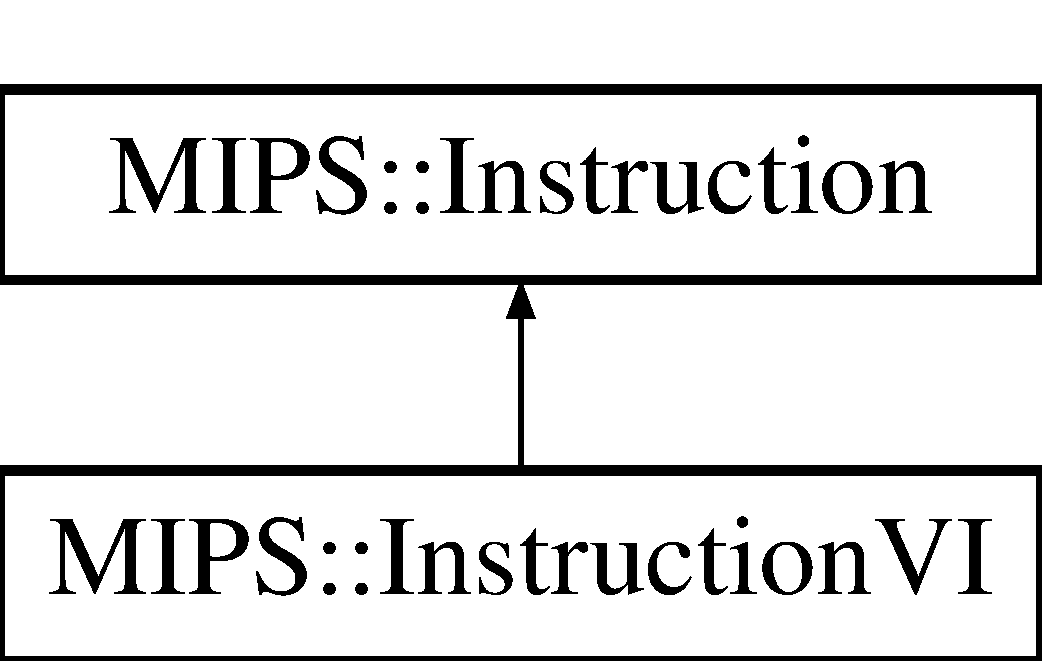
\includegraphics[height=2.000000cm]{classMIPS_1_1InstructionVI}
\end{center}
\end{figure}
\subsection*{Public Member Functions}
\begin{DoxyCompactItemize}
\item 
\hyperlink{classMIPS_1_1InstructionVI_a21d1521859953e06854fd741fbfe22c1}{Instruction\+VI} (\hyperlink{core_8hpp_a6074bae122ae7b527864eec42c728c3c}{bit8\+\_\+t} \hyperlink{classMIPS_1_1Instruction_a45cc6808b5dde8a5d41067d148b55476}{opcode}, \hyperlink{classMIPS_1_1Register}{Register} $\ast$\hyperlink{classMIPS_1_1InstructionVI_a0a48712f3022c8c5731f6d4d371a2515}{rt}, \hyperlink{classMIPS_1_1Register}{Register} $\ast$\hyperlink{classMIPS_1_1InstructionVI_a6d2e8e3afa4cf64d0b08b1907db097f3}{pc})
\item 
virtual \hyperlink{core_8hpp_adc265a970bc35995b5879784bbb3f1b7}{bit16\+\_\+t} \hyperlink{classMIPS_1_1InstructionVI_a0a334d9d507fca448eaa7b0190c17531}{execute} ()=0
\end{DoxyCompactItemize}
\subsection*{Protected Attributes}
\begin{DoxyCompactItemize}
\item 
\hyperlink{classMIPS_1_1Register}{Register} $\ast$ \hyperlink{classMIPS_1_1InstructionVI_a6d2e8e3afa4cf64d0b08b1907db097f3}{pc}
\item 
\hyperlink{classMIPS_1_1Register}{Register} $\ast$ \hyperlink{classMIPS_1_1InstructionVI_a0a48712f3022c8c5731f6d4d371a2515}{rt}
\end{DoxyCompactItemize}


\subsection{Detailed Description}
Classe que representa uma instrução do formato VI do trabalho.

\begin{DoxyAuthor}{Author}
Matheus Nogueira 
\end{DoxyAuthor}


\subsection{Constructor \& Destructor Documentation}
\index{M\+I\+P\+S\+::\+Instruction\+VI@{M\+I\+P\+S\+::\+Instruction\+VI}!Instruction\+VI@{Instruction\+VI}}
\index{Instruction\+VI@{Instruction\+VI}!M\+I\+P\+S\+::\+Instruction\+VI@{M\+I\+P\+S\+::\+Instruction\+VI}}
\subsubsection[{\texorpdfstring{Instruction\+V\+I(bit8\+\_\+t opcode, Register $\ast$rt, Register $\ast$pc)}{InstructionVI(bit8_t opcode, Register *rt, Register *pc)}}]{\setlength{\rightskip}{0pt plus 5cm}M\+I\+P\+S\+::\+Instruction\+V\+I\+::\+Instruction\+VI (
\begin{DoxyParamCaption}
\item[{{\bf bit8\+\_\+t}}]{opcode, }
\item[{{\bf Register} $\ast$}]{rt, }
\item[{{\bf Register} $\ast$}]{pc}
\end{DoxyParamCaption}
)\hspace{0.3cm}{\ttfamily [inline]}}\hypertarget{classMIPS_1_1InstructionVI_a21d1521859953e06854fd741fbfe22c1}{}\label{classMIPS_1_1InstructionVI_a21d1521859953e06854fd741fbfe22c1}
Cria uma nova instrução do formato VI


\begin{DoxyParams}{Parameters}
{\em opcode} & código da operação \\
\hline
{\em rt} & registrador target \\
\hline
{\em pc} & registrador de contador de programa \\
\hline
\end{DoxyParams}


\subsection{Member Function Documentation}
\index{M\+I\+P\+S\+::\+Instruction\+VI@{M\+I\+P\+S\+::\+Instruction\+VI}!execute@{execute}}
\index{execute@{execute}!M\+I\+P\+S\+::\+Instruction\+VI@{M\+I\+P\+S\+::\+Instruction\+VI}}
\subsubsection[{\texorpdfstring{execute()=0}{execute()=0}}]{\setlength{\rightskip}{0pt plus 5cm}virtual {\bf bit16\+\_\+t} M\+I\+P\+S\+::\+Instruction\+V\+I\+::execute (
\begin{DoxyParamCaption}
{}
\end{DoxyParamCaption}
)\hspace{0.3cm}{\ttfamily [pure virtual]}}\hypertarget{classMIPS_1_1InstructionVI_a0a334d9d507fca448eaa7b0190c17531}{}\label{classMIPS_1_1InstructionVI_a0a334d9d507fca448eaa7b0190c17531}
Executa a instrução.

\begin{DoxyReturn}{Returns}
resultado da instrução 
\end{DoxyReturn}


Implements \hyperlink{classMIPS_1_1Instruction_a88668dfaf49dd8608f210ba13948d242}{M\+I\+P\+S\+::\+Instruction}.



\subsection{Member Data Documentation}
\index{M\+I\+P\+S\+::\+Instruction\+VI@{M\+I\+P\+S\+::\+Instruction\+VI}!pc@{pc}}
\index{pc@{pc}!M\+I\+P\+S\+::\+Instruction\+VI@{M\+I\+P\+S\+::\+Instruction\+VI}}
\subsubsection[{\texorpdfstring{pc}{pc}}]{\setlength{\rightskip}{0pt plus 5cm}{\bf Register}$\ast$ M\+I\+P\+S\+::\+Instruction\+V\+I\+::pc\hspace{0.3cm}{\ttfamily [protected]}}\hypertarget{classMIPS_1_1InstructionVI_a6d2e8e3afa4cf64d0b08b1907db097f3}{}\label{classMIPS_1_1InstructionVI_a6d2e8e3afa4cf64d0b08b1907db097f3}
Registrador de contador de programa \index{M\+I\+P\+S\+::\+Instruction\+VI@{M\+I\+P\+S\+::\+Instruction\+VI}!rt@{rt}}
\index{rt@{rt}!M\+I\+P\+S\+::\+Instruction\+VI@{M\+I\+P\+S\+::\+Instruction\+VI}}
\subsubsection[{\texorpdfstring{rt}{rt}}]{\setlength{\rightskip}{0pt plus 5cm}{\bf Register}$\ast$ M\+I\+P\+S\+::\+Instruction\+V\+I\+::rt\hspace{0.3cm}{\ttfamily [protected]}}\hypertarget{classMIPS_1_1InstructionVI_a0a48712f3022c8c5731f6d4d371a2515}{}\label{classMIPS_1_1InstructionVI_a0a48712f3022c8c5731f6d4d371a2515}
Registrador target. 

The documentation for this class was generated from the following file\+:\begin{DoxyCompactItemize}
\item 
include/mips/instructions/\hyperlink{instruction__VI_8hpp}{instruction\+\_\+\+V\+I.\+hpp}\end{DoxyCompactItemize}

\hypertarget{classMIPS_1_1InstructionVII}{}\section{M\+I\+PS\+:\+:Instruction\+V\+II Class Reference}
\label{classMIPS_1_1InstructionVII}\index{M\+I\+P\+S\+::\+Instruction\+V\+II@{M\+I\+P\+S\+::\+Instruction\+V\+II}}


{\ttfamily \#include $<$instruction\+\_\+\+V\+I\+I.\+hpp$>$}

Inheritance diagram for M\+I\+PS\+:\+:Instruction\+V\+II\+:\begin{figure}[H]
\begin{center}
\leavevmode
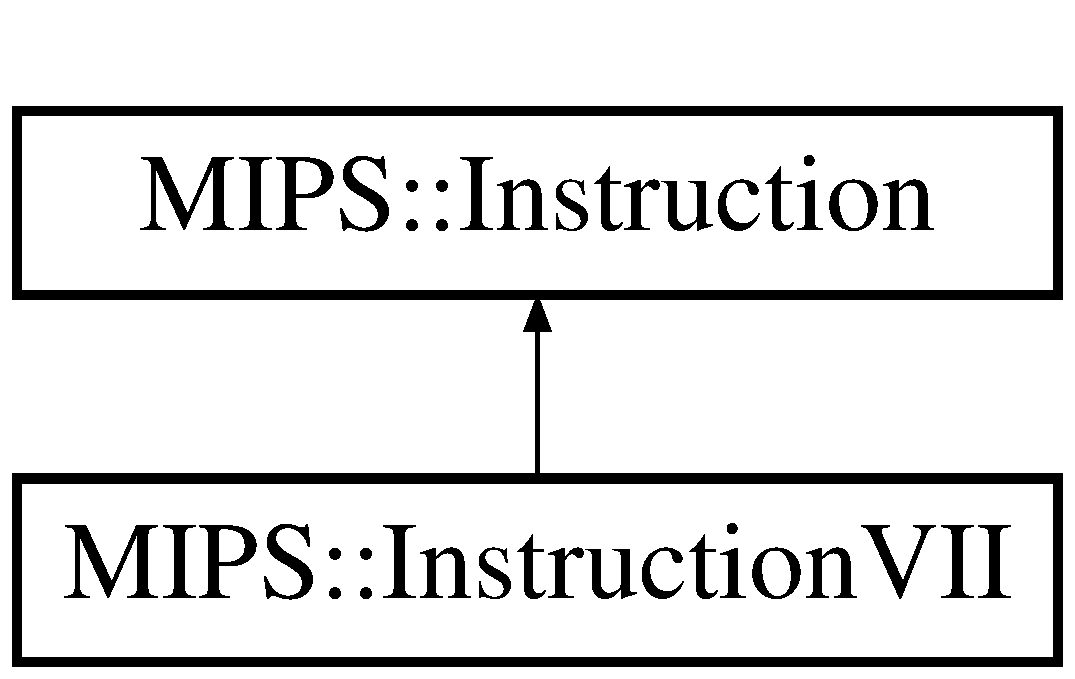
\includegraphics[height=2.000000cm]{classMIPS_1_1InstructionVII}
\end{center}
\end{figure}
\subsection*{Public Member Functions}
\begin{DoxyCompactItemize}
\item 
\hyperlink{classMIPS_1_1InstructionVII_a43d5166f940af6178bd179ea81df6a55}{Instruction\+V\+II} (\hyperlink{core_8hpp_a6074bae122ae7b527864eec42c728c3c}{bit8\+\_\+t} \hyperlink{classMIPS_1_1Instruction_a45cc6808b5dde8a5d41067d148b55476}{opcode}, \hyperlink{classMIPS_1_1Register}{Register} $\ast$\hyperlink{classMIPS_1_1InstructionVII_a8e51202e0b22f8e74668f6de95089e60}{rs}, \hyperlink{classMIPS_1_1Register}{Register} $\ast$\hyperlink{classMIPS_1_1InstructionVII_a8710c06b6e7816f330b0c5daea3402a4}{rt}, \hyperlink{classMIPS_1_1Memory}{Memory} $\ast$\hyperlink{classMIPS_1_1InstructionVII_a4fb34750bedbf137b43f9b55b591e0d7}{memory})
\item 
virtual \hyperlink{core_8hpp_adc265a970bc35995b5879784bbb3f1b7}{bit16\+\_\+t} \hyperlink{classMIPS_1_1InstructionVII_ab004a9cdc0efa7afacb964352abf3ee7}{execute} ()=0
\end{DoxyCompactItemize}
\subsection*{Protected Attributes}
\begin{DoxyCompactItemize}
\item 
\hyperlink{classMIPS_1_1Register}{Register} $\ast$ \hyperlink{classMIPS_1_1InstructionVII_a8e51202e0b22f8e74668f6de95089e60}{rs}
\item 
\hyperlink{classMIPS_1_1Register}{Register} $\ast$ \hyperlink{classMIPS_1_1InstructionVII_a8710c06b6e7816f330b0c5daea3402a4}{rt}
\item 
\hyperlink{classMIPS_1_1Memory}{Memory} $\ast$ \hyperlink{classMIPS_1_1InstructionVII_a4fb34750bedbf137b43f9b55b591e0d7}{memory}
\end{DoxyCompactItemize}


\subsection{Detailed Description}
Classe que representa uma instrução do formato V\+II do trabalho.

\begin{DoxyAuthor}{Author}
Matheus Nogueira 
\end{DoxyAuthor}


\subsection{Constructor \& Destructor Documentation}
\index{M\+I\+P\+S\+::\+Instruction\+V\+II@{M\+I\+P\+S\+::\+Instruction\+V\+II}!Instruction\+V\+II@{Instruction\+V\+II}}
\index{Instruction\+V\+II@{Instruction\+V\+II}!M\+I\+P\+S\+::\+Instruction\+V\+II@{M\+I\+P\+S\+::\+Instruction\+V\+II}}
\subsubsection[{\texorpdfstring{Instruction\+V\+I\+I(bit8\+\_\+t opcode, Register $\ast$rs, Register $\ast$rt, Memory $\ast$memory)}{InstructionVII(bit8_t opcode, Register *rs, Register *rt, Memory *memory)}}]{\setlength{\rightskip}{0pt plus 5cm}M\+I\+P\+S\+::\+Instruction\+V\+I\+I\+::\+Instruction\+V\+II (
\begin{DoxyParamCaption}
\item[{{\bf bit8\+\_\+t}}]{opcode, }
\item[{{\bf Register} $\ast$}]{rs, }
\item[{{\bf Register} $\ast$}]{rt, }
\item[{{\bf Memory} $\ast$}]{memory}
\end{DoxyParamCaption}
)\hspace{0.3cm}{\ttfamily [inline]}}\hypertarget{classMIPS_1_1InstructionVII_a43d5166f940af6178bd179ea81df6a55}{}\label{classMIPS_1_1InstructionVII_a43d5166f940af6178bd179ea81df6a55}
Cria uma nova instrução do formato V\+II


\begin{DoxyParams}{Parameters}
{\em opcode} & código da operação \\
\hline
{\em rs} & registrador destination \\
\hline
{\em rt} & registrador target \\
\hline
{\em memory} & unidade de memória do processador \\
\hline
\end{DoxyParams}


\subsection{Member Function Documentation}
\index{M\+I\+P\+S\+::\+Instruction\+V\+II@{M\+I\+P\+S\+::\+Instruction\+V\+II}!execute@{execute}}
\index{execute@{execute}!M\+I\+P\+S\+::\+Instruction\+V\+II@{M\+I\+P\+S\+::\+Instruction\+V\+II}}
\subsubsection[{\texorpdfstring{execute()=0}{execute()=0}}]{\setlength{\rightskip}{0pt plus 5cm}virtual {\bf bit16\+\_\+t} M\+I\+P\+S\+::\+Instruction\+V\+I\+I\+::execute (
\begin{DoxyParamCaption}
{}
\end{DoxyParamCaption}
)\hspace{0.3cm}{\ttfamily [pure virtual]}}\hypertarget{classMIPS_1_1InstructionVII_ab004a9cdc0efa7afacb964352abf3ee7}{}\label{classMIPS_1_1InstructionVII_ab004a9cdc0efa7afacb964352abf3ee7}
Executa a instrução.

\begin{DoxyReturn}{Returns}
resultado da instrução 
\end{DoxyReturn}


Implements \hyperlink{classMIPS_1_1Instruction_a88668dfaf49dd8608f210ba13948d242}{M\+I\+P\+S\+::\+Instruction}.



\subsection{Member Data Documentation}
\index{M\+I\+P\+S\+::\+Instruction\+V\+II@{M\+I\+P\+S\+::\+Instruction\+V\+II}!memory@{memory}}
\index{memory@{memory}!M\+I\+P\+S\+::\+Instruction\+V\+II@{M\+I\+P\+S\+::\+Instruction\+V\+II}}
\subsubsection[{\texorpdfstring{memory}{memory}}]{\setlength{\rightskip}{0pt plus 5cm}{\bf Memory}$\ast$ M\+I\+P\+S\+::\+Instruction\+V\+I\+I\+::memory\hspace{0.3cm}{\ttfamily [protected]}}\hypertarget{classMIPS_1_1InstructionVII_a4fb34750bedbf137b43f9b55b591e0d7}{}\label{classMIPS_1_1InstructionVII_a4fb34750bedbf137b43f9b55b591e0d7}
Unidade de memória usada para acessar os dados. \index{M\+I\+P\+S\+::\+Instruction\+V\+II@{M\+I\+P\+S\+::\+Instruction\+V\+II}!rs@{rs}}
\index{rs@{rs}!M\+I\+P\+S\+::\+Instruction\+V\+II@{M\+I\+P\+S\+::\+Instruction\+V\+II}}
\subsubsection[{\texorpdfstring{rs}{rs}}]{\setlength{\rightskip}{0pt plus 5cm}{\bf Register}$\ast$ M\+I\+P\+S\+::\+Instruction\+V\+I\+I\+::rs\hspace{0.3cm}{\ttfamily [protected]}}\hypertarget{classMIPS_1_1InstructionVII_a8e51202e0b22f8e74668f6de95089e60}{}\label{classMIPS_1_1InstructionVII_a8e51202e0b22f8e74668f6de95089e60}
Registrador source \index{M\+I\+P\+S\+::\+Instruction\+V\+II@{M\+I\+P\+S\+::\+Instruction\+V\+II}!rt@{rt}}
\index{rt@{rt}!M\+I\+P\+S\+::\+Instruction\+V\+II@{M\+I\+P\+S\+::\+Instruction\+V\+II}}
\subsubsection[{\texorpdfstring{rt}{rt}}]{\setlength{\rightskip}{0pt plus 5cm}{\bf Register}$\ast$ M\+I\+P\+S\+::\+Instruction\+V\+I\+I\+::rt\hspace{0.3cm}{\ttfamily [protected]}}\hypertarget{classMIPS_1_1InstructionVII_a8710c06b6e7816f330b0c5daea3402a4}{}\label{classMIPS_1_1InstructionVII_a8710c06b6e7816f330b0c5daea3402a4}
Registrador target. 

The documentation for this class was generated from the following file\+:\begin{DoxyCompactItemize}
\item 
include/mips/instructions/\hyperlink{instruction__VII_8hpp}{instruction\+\_\+\+V\+I\+I.\+hpp}\end{DoxyCompactItemize}

\hypertarget{classMIPS_1_1Interpreter}{}\section{M\+I\+PS\+:\+:Interpreter Class Reference}
\label{classMIPS_1_1Interpreter}\index{M\+I\+P\+S\+::\+Interpreter@{M\+I\+P\+S\+::\+Interpreter}}


{\ttfamily \#include $<$interpreter.\+hpp$>$}

\subsection*{Public Member Functions}
\begin{DoxyCompactItemize}
\item 
\hyperlink{classMIPS_1_1Interpreter_a885d19e6aba129b6e8e009b9315b27a2}{Interpreter} (const char $\ast$file)
\item 
\hyperlink{classMIPS_1_1Interpreter_a41cc557c63eaedc2227de15df4a965b7}{$\sim$\+Interpreter} ()
\item 
void \hyperlink{classMIPS_1_1Interpreter_ad530eb79becefe55e07d1e6c084f7e5d}{compile} ()
\item 
bool \hyperlink{classMIPS_1_1Interpreter_a9b27efdc3235bde933c65acc53ae02d0}{ok} ()
\end{DoxyCompactItemize}


\subsection{Detailed Description}
Classe responsável por receber um texto e criar instruções 16 bits correspondentes para a arquitetura M\+I\+PS 32.

\begin{DoxyAuthor}{Author}
Matheus Nogueira 
\end{DoxyAuthor}


\subsection{Constructor \& Destructor Documentation}
\index{M\+I\+P\+S\+::\+Interpreter@{M\+I\+P\+S\+::\+Interpreter}!Interpreter@{Interpreter}}
\index{Interpreter@{Interpreter}!M\+I\+P\+S\+::\+Interpreter@{M\+I\+P\+S\+::\+Interpreter}}
\subsubsection[{\texorpdfstring{Interpreter(const char $\ast$file)}{Interpreter(const char *file)}}]{\setlength{\rightskip}{0pt plus 5cm}M\+I\+P\+S\+::\+Interpreter\+::\+Interpreter (
\begin{DoxyParamCaption}
\item[{const char $\ast$}]{file}
\end{DoxyParamCaption}
)}\hypertarget{classMIPS_1_1Interpreter_a885d19e6aba129b6e8e009b9315b27a2}{}\label{classMIPS_1_1Interpreter_a885d19e6aba129b6e8e009b9315b27a2}
Cria uma nova instância do interpretador.


\begin{DoxyParams}{Parameters}
{\em file} & arquivo que será interpretado. \\
\hline
\end{DoxyParams}
\index{M\+I\+P\+S\+::\+Interpreter@{M\+I\+P\+S\+::\+Interpreter}!````~Interpreter@{$\sim$\+Interpreter}}
\index{````~Interpreter@{$\sim$\+Interpreter}!M\+I\+P\+S\+::\+Interpreter@{M\+I\+P\+S\+::\+Interpreter}}
\subsubsection[{\texorpdfstring{$\sim$\+Interpreter()}{~Interpreter()}}]{\setlength{\rightskip}{0pt plus 5cm}M\+I\+P\+S\+::\+Interpreter\+::$\sim$\+Interpreter (
\begin{DoxyParamCaption}
{}
\end{DoxyParamCaption}
)}\hypertarget{classMIPS_1_1Interpreter_a41cc557c63eaedc2227de15df4a965b7}{}\label{classMIPS_1_1Interpreter_a41cc557c63eaedc2227de15df4a965b7}
Destroi o interpretador. 

\subsection{Member Function Documentation}
\index{M\+I\+P\+S\+::\+Interpreter@{M\+I\+P\+S\+::\+Interpreter}!compile@{compile}}
\index{compile@{compile}!M\+I\+P\+S\+::\+Interpreter@{M\+I\+P\+S\+::\+Interpreter}}
\subsubsection[{\texorpdfstring{compile()}{compile()}}]{\setlength{\rightskip}{0pt plus 5cm}void M\+I\+P\+S\+::\+Interpreter\+::compile (
\begin{DoxyParamCaption}
{}
\end{DoxyParamCaption}
)}\hypertarget{classMIPS_1_1Interpreter_ad530eb79becefe55e07d1e6c084f7e5d}{}\label{classMIPS_1_1Interpreter_ad530eb79becefe55e07d1e6c084f7e5d}
Processa o arquivo de entrada para que ele possa ser interpretado. \index{M\+I\+P\+S\+::\+Interpreter@{M\+I\+P\+S\+::\+Interpreter}!ok@{ok}}
\index{ok@{ok}!M\+I\+P\+S\+::\+Interpreter@{M\+I\+P\+S\+::\+Interpreter}}
\subsubsection[{\texorpdfstring{ok()}{ok()}}]{\setlength{\rightskip}{0pt plus 5cm}bool M\+I\+P\+S\+::\+Interpreter\+::ok (
\begin{DoxyParamCaption}
{}
\end{DoxyParamCaption}
)\hspace{0.3cm}{\ttfamily [inline]}}\hypertarget{classMIPS_1_1Interpreter_a9b27efdc3235bde933c65acc53ae02d0}{}\label{classMIPS_1_1Interpreter_a9b27efdc3235bde933c65acc53ae02d0}
Checa se o interpretador encontrou algum erro durante a sua execução. Se sim, retorna false.

\begin{DoxyReturn}{Returns}
true se o interpretador realizou sem papel sem erros. 
\end{DoxyReturn}


The documentation for this class was generated from the following file\+:\begin{DoxyCompactItemize}
\item 
include/mips/interpreter/\hyperlink{interpreter_8hpp}{interpreter.\+hpp}\end{DoxyCompactItemize}

\hypertarget{classMIPS_1_1InterpreterException}{}\section{M\+I\+PS\+:\+:Interpreter\+Exception Class Reference}
\label{classMIPS_1_1InterpreterException}\index{M\+I\+P\+S\+::\+Interpreter\+Exception@{M\+I\+P\+S\+::\+Interpreter\+Exception}}


{\ttfamily \#include $<$interpreter\+\_\+exception.\+hpp$>$}

Inheritance diagram for M\+I\+PS\+:\+:Interpreter\+Exception\+:\begin{figure}[H]
\begin{center}
\leavevmode
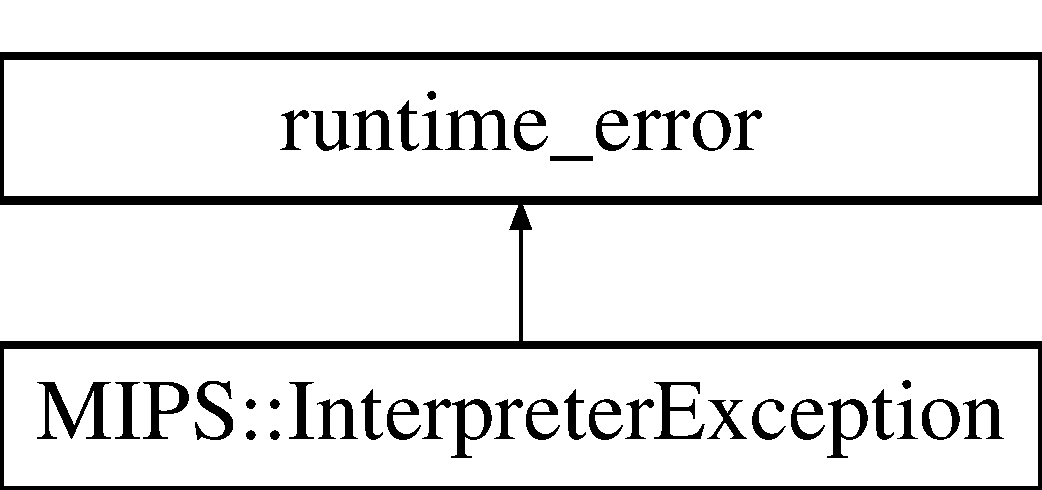
\includegraphics[height=2.000000cm]{classMIPS_1_1InterpreterException}
\end{center}
\end{figure}
\subsection*{Public Member Functions}
\begin{DoxyCompactItemize}
\item 
\hyperlink{classMIPS_1_1InterpreterException_a8c3cc0b526ddeca99eee51bfbf353549}{Interpreter\+Exception} (const char $\ast$msg, \hyperlink{core_8hpp_a6074bae122ae7b527864eec42c728c3c}{bit8\+\_\+t} opcode)
\item 
virtual const char $\ast$ \hyperlink{classMIPS_1_1InterpreterException_a7ddaf2edf53aaaf5b0ad995635033003}{what} () const   throw ()
\item 
\hyperlink{core_8hpp_a6074bae122ae7b527864eec42c728c3c}{bit8\+\_\+t} \hyperlink{classMIPS_1_1InterpreterException_a6d2fc264fb6b9c61bf9690747d1bf5b6}{get\+Code} ()
\end{DoxyCompactItemize}


\subsection{Detailed Description}
Exceção que é lançada pelo interpretador quando um erro é encontrado no arquivo fonte.

\begin{DoxyAuthor}{Author}
Matheus Nogueira 
\end{DoxyAuthor}


\subsection{Constructor \& Destructor Documentation}
\index{M\+I\+P\+S\+::\+Interpreter\+Exception@{M\+I\+P\+S\+::\+Interpreter\+Exception}!Interpreter\+Exception@{Interpreter\+Exception}}
\index{Interpreter\+Exception@{Interpreter\+Exception}!M\+I\+P\+S\+::\+Interpreter\+Exception@{M\+I\+P\+S\+::\+Interpreter\+Exception}}
\subsubsection[{\texorpdfstring{Interpreter\+Exception(const char $\ast$msg, bit8\+\_\+t opcode)}{InterpreterException(const char *msg, bit8_t opcode)}}]{\setlength{\rightskip}{0pt plus 5cm}M\+I\+P\+S\+::\+Interpreter\+Exception\+::\+Interpreter\+Exception (
\begin{DoxyParamCaption}
\item[{const char $\ast$}]{msg, }
\item[{{\bf bit8\+\_\+t}}]{opcode}
\end{DoxyParamCaption}
)\hspace{0.3cm}{\ttfamily [inline]}}\hypertarget{classMIPS_1_1InterpreterException_a8c3cc0b526ddeca99eee51bfbf353549}{}\label{classMIPS_1_1InterpreterException_a8c3cc0b526ddeca99eee51bfbf353549}
Cria uma nova exceção.


\begin{DoxyParams}{Parameters}
{\em msg} & mensagem de erro. \\
\hline
{\em opcode} & código do erro. \\
\hline
\end{DoxyParams}


\subsection{Member Function Documentation}
\index{M\+I\+P\+S\+::\+Interpreter\+Exception@{M\+I\+P\+S\+::\+Interpreter\+Exception}!get\+Code@{get\+Code}}
\index{get\+Code@{get\+Code}!M\+I\+P\+S\+::\+Interpreter\+Exception@{M\+I\+P\+S\+::\+Interpreter\+Exception}}
\subsubsection[{\texorpdfstring{get\+Code()}{getCode()}}]{\setlength{\rightskip}{0pt plus 5cm}{\bf bit8\+\_\+t} M\+I\+P\+S\+::\+Interpreter\+Exception\+::get\+Code (
\begin{DoxyParamCaption}
{}
\end{DoxyParamCaption}
)\hspace{0.3cm}{\ttfamily [inline]}}\hypertarget{classMIPS_1_1InterpreterException_a6d2fc264fb6b9c61bf9690747d1bf5b6}{}\label{classMIPS_1_1InterpreterException_a6d2fc264fb6b9c61bf9690747d1bf5b6}
Retorna o codigo de operação da exceção.

\begin{DoxyReturn}{Returns}
codigo de operação. 
\end{DoxyReturn}
\index{M\+I\+P\+S\+::\+Interpreter\+Exception@{M\+I\+P\+S\+::\+Interpreter\+Exception}!what@{what}}
\index{what@{what}!M\+I\+P\+S\+::\+Interpreter\+Exception@{M\+I\+P\+S\+::\+Interpreter\+Exception}}
\subsubsection[{\texorpdfstring{what() const }{what() const }}]{\setlength{\rightskip}{0pt plus 5cm}virtual const char$\ast$ M\+I\+P\+S\+::\+Interpreter\+Exception\+::what (
\begin{DoxyParamCaption}
{}
\end{DoxyParamCaption}
) const throw  ) \hspace{0.3cm}{\ttfamily [inline]}, {\ttfamily [virtual]}}\hypertarget{classMIPS_1_1InterpreterException_a7ddaf2edf53aaaf5b0ad995635033003}{}\label{classMIPS_1_1InterpreterException_a7ddaf2edf53aaaf5b0ad995635033003}
Retorna a mensagem de erro.

\begin{DoxyReturn}{Returns}
mensagem de erro. 
\end{DoxyReturn}


The documentation for this class was generated from the following file\+:\begin{DoxyCompactItemize}
\item 
include/mips/interpreter/exception/\hyperlink{interpreter__exception_8hpp}{interpreter\+\_\+exception.\+hpp}\end{DoxyCompactItemize}

\hypertarget{classMIPS_1_1JtZeroInstruction}{}\section{M\+I\+PS\+:\+:Jt\+Zero\+Instruction Class Reference}
\label{classMIPS_1_1JtZeroInstruction}\index{M\+I\+P\+S\+::\+Jt\+Zero\+Instruction@{M\+I\+P\+S\+::\+Jt\+Zero\+Instruction}}


{\ttfamily \#include $<$jt\+\_\+zero.\+hpp$>$}

Inheritance diagram for M\+I\+PS\+:\+:Jt\+Zero\+Instruction\+:\begin{figure}[H]
\begin{center}
\leavevmode
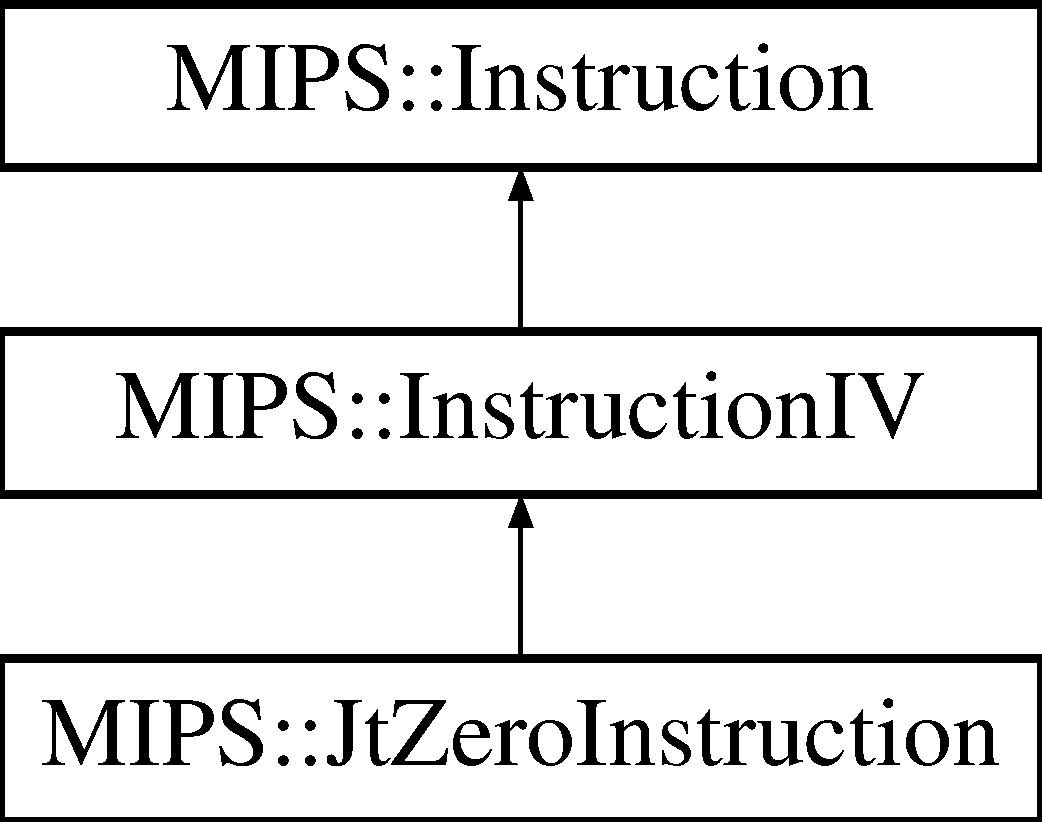
\includegraphics[height=3.000000cm]{classMIPS_1_1JtZeroInstruction}
\end{center}
\end{figure}
\subsection*{Public Member Functions}
\begin{DoxyCompactItemize}
\item 
\hyperlink{classMIPS_1_1JtZeroInstruction_a2968f65f63844b0f2afb5cea2bbcc910}{Jt\+Zero\+Instruction} (\hyperlink{core_8hpp_a6074bae122ae7b527864eec42c728c3c}{bit8\+\_\+t} \hyperlink{classMIPS_1_1Instruction_a45cc6808b5dde8a5d41067d148b55476}{opcode}, struct \hyperlink{structMIPS_1_1ALUFlags}{A\+L\+U\+Flags} \&alu\+Flags, \hyperlink{core_8hpp_a6074bae122ae7b527864eec42c728c3c}{bit8\+\_\+t} \hyperlink{classMIPS_1_1InstructionIV_abcb91e65c800a41bf9c46b5770120b36}{offset})
\item 
\hyperlink{core_8hpp_adc265a970bc35995b5879784bbb3f1b7}{bit16\+\_\+t} \hyperlink{classMIPS_1_1JtZeroInstruction_a8a56439dd5df5fcf00344304b8409e45}{execute} ()
\end{DoxyCompactItemize}
\subsection*{Additional Inherited Members}


\subsection{Detailed Description}
Instrução que faz o desvio se a flag zero da A\+LU está setada como 1.

\begin{DoxyAuthor}{Author}
Matheus Nogueira 
\end{DoxyAuthor}


\subsection{Constructor \& Destructor Documentation}
\index{M\+I\+P\+S\+::\+Jt\+Zero\+Instruction@{M\+I\+P\+S\+::\+Jt\+Zero\+Instruction}!Jt\+Zero\+Instruction@{Jt\+Zero\+Instruction}}
\index{Jt\+Zero\+Instruction@{Jt\+Zero\+Instruction}!M\+I\+P\+S\+::\+Jt\+Zero\+Instruction@{M\+I\+P\+S\+::\+Jt\+Zero\+Instruction}}
\subsubsection[{\texorpdfstring{Jt\+Zero\+Instruction(bit8\+\_\+t opcode, struct A\+L\+U\+Flags \&alu\+Flags, bit8\+\_\+t offset)}{JtZeroInstruction(bit8_t opcode, struct ALUFlags &aluFlags, bit8_t offset)}}]{\setlength{\rightskip}{0pt plus 5cm}M\+I\+P\+S\+::\+Jt\+Zero\+Instruction\+::\+Jt\+Zero\+Instruction (
\begin{DoxyParamCaption}
\item[{{\bf bit8\+\_\+t}}]{opcode, }
\item[{struct {\bf A\+L\+U\+Flags} \&}]{alu\+Flags, }
\item[{{\bf bit8\+\_\+t}}]{offset}
\end{DoxyParamCaption}
)\hspace{0.3cm}{\ttfamily [inline]}}\hypertarget{classMIPS_1_1JtZeroInstruction_a2968f65f63844b0f2afb5cea2bbcc910}{}\label{classMIPS_1_1JtZeroInstruction_a2968f65f63844b0f2afb5cea2bbcc910}
Cria uma instrução de jump on true.


\begin{DoxyParams}{Parameters}
{\em opcode} & código da operação \\
\hline
{\em alu\+Flags} & objeto de flags da A\+LU \\
\hline
{\em offset} & offset de 11 bits \\
\hline
\end{DoxyParams}


\subsection{Member Function Documentation}
\index{M\+I\+P\+S\+::\+Jt\+Zero\+Instruction@{M\+I\+P\+S\+::\+Jt\+Zero\+Instruction}!execute@{execute}}
\index{execute@{execute}!M\+I\+P\+S\+::\+Jt\+Zero\+Instruction@{M\+I\+P\+S\+::\+Jt\+Zero\+Instruction}}
\subsubsection[{\texorpdfstring{execute()}{execute()}}]{\setlength{\rightskip}{0pt plus 5cm}{\bf bit16\+\_\+t} M\+I\+P\+S\+::\+Jt\+Zero\+Instruction\+::execute (
\begin{DoxyParamCaption}
{}
\end{DoxyParamCaption}
)\hspace{0.3cm}{\ttfamily [virtual]}}\hypertarget{classMIPS_1_1JtZeroInstruction_a8a56439dd5df5fcf00344304b8409e45}{}\label{classMIPS_1_1JtZeroInstruction_a8a56439dd5df5fcf00344304b8409e45}
Executa a instrução.

\begin{DoxyReturn}{Returns}
returna 0 se o desvio não for tomado, 1 se desvio for tomado. 
\end{DoxyReturn}


Implements \hyperlink{classMIPS_1_1InstructionIV_ae9eeb2c1aa5392cc3e2d9f2d816b799c}{M\+I\+P\+S\+::\+Instruction\+IV}.



The documentation for this class was generated from the following file\+:\begin{DoxyCompactItemize}
\item 
include/mips/instructions/format\+\_\+\+I\+V/jt\+\_\+zero.\+hpp\end{DoxyCompactItemize}

\hypertarget{classMIPS_1_1JumpInstruction}{}\section{M\+I\+PS\+:\+:Jump\+Instruction Class Reference}
\label{classMIPS_1_1JumpInstruction}\index{M\+I\+P\+S\+::\+Jump\+Instruction@{M\+I\+P\+S\+::\+Jump\+Instruction}}


{\ttfamily \#include $<$j.\+hpp$>$}

Inheritance diagram for M\+I\+PS\+:\+:Jump\+Instruction\+:\begin{figure}[H]
\begin{center}
\leavevmode
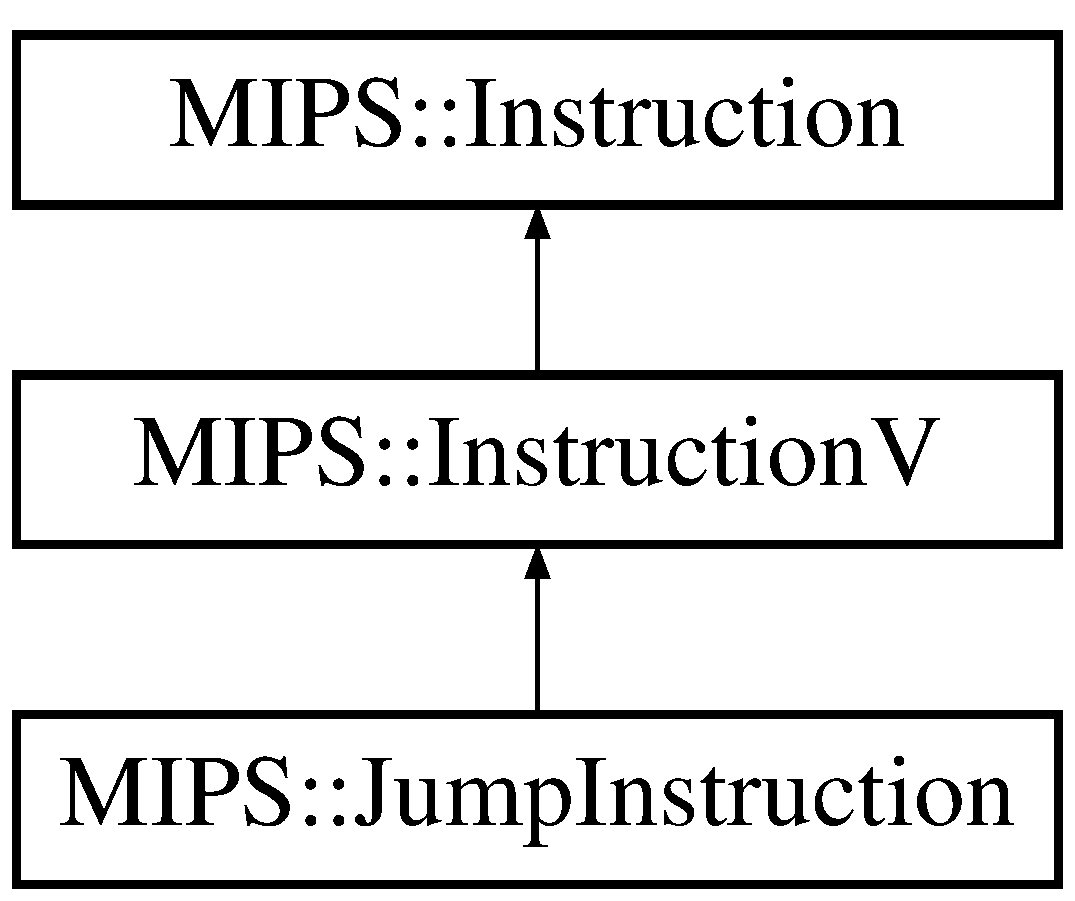
\includegraphics[height=3.000000cm]{classMIPS_1_1JumpInstruction}
\end{center}
\end{figure}
\subsection*{Public Member Functions}
\begin{DoxyCompactItemize}
\item 
\hyperlink{classMIPS_1_1JumpInstruction_a5688d5a7c2ded2c3b8a32cb395cb9db9}{Jump\+Instruction} (\hyperlink{core_8hpp_a6074bae122ae7b527864eec42c728c3c}{bit8\+\_\+t} \hyperlink{classMIPS_1_1Instruction_a45cc6808b5dde8a5d41067d148b55476}{opcode}, \hyperlink{core_8hpp_adc265a970bc35995b5879784bbb3f1b7}{bit16\+\_\+t} \hyperlink{classMIPS_1_1InstructionV_ac2e294fde4971aa6a149480f22ae29e9}{offset})
\item 
\hyperlink{core_8hpp_adc265a970bc35995b5879784bbb3f1b7}{bit16\+\_\+t} \hyperlink{classMIPS_1_1JumpInstruction_a843961af93d20e35dd1fab6bf341e16e}{execute} ()
\end{DoxyCompactItemize}
\subsection*{Additional Inherited Members}


\subsection{Detailed Description}
Instrução que faz o desvio se a flag zero da A\+LU está setada como 1.

\begin{DoxyAuthor}{Author}
Matheus Nogueira 
\end{DoxyAuthor}


\subsection{Constructor \& Destructor Documentation}
\index{M\+I\+P\+S\+::\+Jump\+Instruction@{M\+I\+P\+S\+::\+Jump\+Instruction}!Jump\+Instruction@{Jump\+Instruction}}
\index{Jump\+Instruction@{Jump\+Instruction}!M\+I\+P\+S\+::\+Jump\+Instruction@{M\+I\+P\+S\+::\+Jump\+Instruction}}
\subsubsection[{\texorpdfstring{Jump\+Instruction(bit8\+\_\+t opcode, bit16\+\_\+t offset)}{JumpInstruction(bit8_t opcode, bit16_t offset)}}]{\setlength{\rightskip}{0pt plus 5cm}M\+I\+P\+S\+::\+Jump\+Instruction\+::\+Jump\+Instruction (
\begin{DoxyParamCaption}
\item[{{\bf bit8\+\_\+t}}]{opcode, }
\item[{{\bf bit16\+\_\+t}}]{offset}
\end{DoxyParamCaption}
)\hspace{0.3cm}{\ttfamily [inline]}}\hypertarget{classMIPS_1_1JumpInstruction_a5688d5a7c2ded2c3b8a32cb395cb9db9}{}\label{classMIPS_1_1JumpInstruction_a5688d5a7c2ded2c3b8a32cb395cb9db9}
Cria uma instrução de jump.


\begin{DoxyParams}{Parameters}
{\em opcode} & código da operação \\
\hline
{\em offset} & offset de 12 bits \\
\hline
\end{DoxyParams}


\subsection{Member Function Documentation}
\index{M\+I\+P\+S\+::\+Jump\+Instruction@{M\+I\+P\+S\+::\+Jump\+Instruction}!execute@{execute}}
\index{execute@{execute}!M\+I\+P\+S\+::\+Jump\+Instruction@{M\+I\+P\+S\+::\+Jump\+Instruction}}
\subsubsection[{\texorpdfstring{execute()}{execute()}}]{\setlength{\rightskip}{0pt plus 5cm}{\bf bit16\+\_\+t} M\+I\+P\+S\+::\+Jump\+Instruction\+::execute (
\begin{DoxyParamCaption}
{}
\end{DoxyParamCaption}
)\hspace{0.3cm}{\ttfamily [virtual]}}\hypertarget{classMIPS_1_1JumpInstruction_a843961af93d20e35dd1fab6bf341e16e}{}\label{classMIPS_1_1JumpInstruction_a843961af93d20e35dd1fab6bf341e16e}
Executa a instrução.

\begin{DoxyReturn}{Returns}
returna 0 se o desvio não for tomado, 1 se desvio for tomado. 
\end{DoxyReturn}


Implements \hyperlink{classMIPS_1_1InstructionV_a511d8ba098bcca95f1e91ff6616470ef}{M\+I\+P\+S\+::\+InstructionV}.



The documentation for this class was generated from the following file\+:\begin{DoxyCompactItemize}
\item 
include/mips/instructions/format\+\_\+\+V/\hyperlink{j_8hpp}{j.\+hpp}\end{DoxyCompactItemize}

\hypertarget{structMIPS_1_1Label}{}\section{M\+I\+PS\+:\+:Label Struct Reference}
\label{structMIPS_1_1Label}\index{M\+I\+P\+S\+::\+Label@{M\+I\+P\+S\+::\+Label}}


{\ttfamily \#include $<$label.\+hpp$>$}

\subsection*{Public Attributes}
\begin{DoxyCompactItemize}
\item 
char \hyperlink{structMIPS_1_1Label_aeb046f4a05c4ab7c02a87b49bd75de51}{label} \mbox{[}64\mbox{]}\hypertarget{structMIPS_1_1Label_aeb046f4a05c4ab7c02a87b49bd75de51}{}\label{structMIPS_1_1Label_aeb046f4a05c4ab7c02a87b49bd75de51}

\begin{DoxyCompactList}\small\item\em Nome do label. \end{DoxyCompactList}\item 
unsigned long \hyperlink{structMIPS_1_1Label_a1e25037de487a7b1bbe4840e872024b0}{line}\hypertarget{structMIPS_1_1Label_a1e25037de487a7b1bbe4840e872024b0}{}\label{structMIPS_1_1Label_a1e25037de487a7b1bbe4840e872024b0}

\begin{DoxyCompactList}\small\item\em Linha que ele está definido. \end{DoxyCompactList}\end{DoxyCompactItemize}


\subsection{Detailed Description}
Estrutura que armazena o nome do label e a linha que ele se encontra. 

The documentation for this struct was generated from the following file\+:\begin{DoxyCompactItemize}
\item 
include/mips/interpreter/\hyperlink{label_8hpp}{label.\+hpp}\end{DoxyCompactItemize}

\hypertarget{classMIPS_1_1LchInstruction}{}\section{M\+I\+PS\+:\+:Lch\+Instruction Class Reference}
\label{classMIPS_1_1LchInstruction}\index{M\+I\+P\+S\+::\+Lch\+Instruction@{M\+I\+P\+S\+::\+Lch\+Instruction}}


{\ttfamily \#include $<$lch.\+hpp$>$}

Inheritance diagram for M\+I\+PS\+:\+:Lch\+Instruction\+:\begin{figure}[H]
\begin{center}
\leavevmode
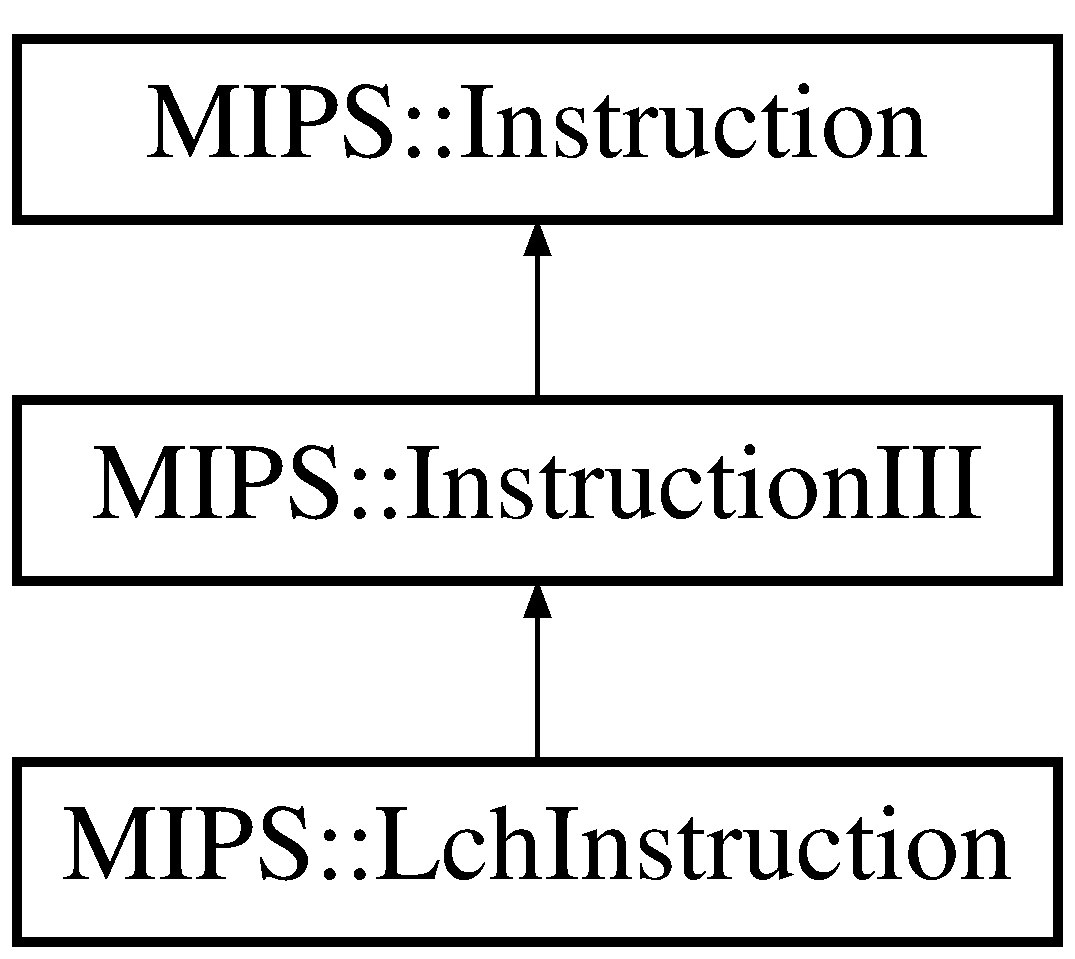
\includegraphics[height=3.000000cm]{classMIPS_1_1LchInstruction}
\end{center}
\end{figure}
\subsection*{Public Member Functions}
\begin{DoxyCompactItemize}
\item 
\hyperlink{classMIPS_1_1LchInstruction_a6e565d4fb7708e974d0e475bd3fabfa7}{Lch\+Instruction} (\hyperlink{core_8hpp_a6074bae122ae7b527864eec42c728c3c}{bit8\+\_\+t} \hyperlink{classMIPS_1_1Instruction_a45cc6808b5dde8a5d41067d148b55476}{opcode}, \hyperlink{classMIPS_1_1Register}{Register} $\ast$\hyperlink{classMIPS_1_1InstructionIII_a76e7b218fc57cd2fc559bf72498090b6}{rd}, \hyperlink{core_8hpp_a6074bae122ae7b527864eec42c728c3c}{bit8\+\_\+t} \hyperlink{classMIPS_1_1InstructionIII_ad0ebd3b6e7594fc583e9a409bf99a6c7}{offset})
\item 
\hyperlink{core_8hpp_adc265a970bc35995b5879784bbb3f1b7}{bit16\+\_\+t} \hyperlink{classMIPS_1_1LchInstruction_a6dad60c9189a1e84fd7c789b9642077d}{execute} ()
\end{DoxyCompactItemize}
\subsection*{Additional Inherited Members}


\subsection{Detailed Description}
Instrução utilizada para carregar 8 bits e carregá-\/los em um no bit mais significativo do registrador definido pelo programador.

\begin{DoxyAuthor}{Author}
Matheus Nogueira 
\end{DoxyAuthor}


\subsection{Constructor \& Destructor Documentation}
\index{M\+I\+P\+S\+::\+Lch\+Instruction@{M\+I\+P\+S\+::\+Lch\+Instruction}!Lch\+Instruction@{Lch\+Instruction}}
\index{Lch\+Instruction@{Lch\+Instruction}!M\+I\+P\+S\+::\+Lch\+Instruction@{M\+I\+P\+S\+::\+Lch\+Instruction}}
\subsubsection[{\texorpdfstring{Lch\+Instruction(bit8\+\_\+t opcode, Register $\ast$rd, bit8\+\_\+t offset)}{LchInstruction(bit8_t opcode, Register *rd, bit8_t offset)}}]{\setlength{\rightskip}{0pt plus 5cm}M\+I\+P\+S\+::\+Lch\+Instruction\+::\+Lch\+Instruction (
\begin{DoxyParamCaption}
\item[{{\bf bit8\+\_\+t}}]{opcode, }
\item[{{\bf Register} $\ast$}]{rd, }
\item[{{\bf bit8\+\_\+t}}]{offset}
\end{DoxyParamCaption}
)\hspace{0.3cm}{\ttfamily [inline]}}\hypertarget{classMIPS_1_1LchInstruction_a6e565d4fb7708e974d0e475bd3fabfa7}{}\label{classMIPS_1_1LchInstruction_a6e565d4fb7708e974d0e475bd3fabfa7}
Cria uma instrução de lhc.


\begin{DoxyParams}{Parameters}
{\em opcode} & código da operação \\
\hline
{\em rd} & registrador rd \\
\hline
{\em offset} & offset de 11 bits \\
\hline
\end{DoxyParams}


\subsection{Member Function Documentation}
\index{M\+I\+P\+S\+::\+Lch\+Instruction@{M\+I\+P\+S\+::\+Lch\+Instruction}!execute@{execute}}
\index{execute@{execute}!M\+I\+P\+S\+::\+Lch\+Instruction@{M\+I\+P\+S\+::\+Lch\+Instruction}}
\subsubsection[{\texorpdfstring{execute()}{execute()}}]{\setlength{\rightskip}{0pt plus 5cm}{\bf bit16\+\_\+t} M\+I\+P\+S\+::\+Lch\+Instruction\+::execute (
\begin{DoxyParamCaption}
{}
\end{DoxyParamCaption}
)\hspace{0.3cm}{\ttfamily [virtual]}}\hypertarget{classMIPS_1_1LchInstruction_a6dad60c9189a1e84fd7c789b9642077d}{}\label{classMIPS_1_1LchInstruction_a6dad60c9189a1e84fd7c789b9642077d}
Executa a instrução.

\begin{DoxyReturn}{Returns}
resultado da operação 
\end{DoxyReturn}


Implements \hyperlink{classMIPS_1_1InstructionIII_aee3071c23abc542e55b446abee766c5e}{M\+I\+P\+S\+::\+Instruction\+I\+II}.



The documentation for this class was generated from the following file\+:\begin{DoxyCompactItemize}
\item 
include/mips/instructions/format\+\_\+\+I\+I\+I/\hyperlink{lch_8hpp}{lch.\+hpp}\end{DoxyCompactItemize}

\hypertarget{classMIPS_1_1LclInstruction}{}\section{M\+I\+PS\+:\+:Lcl\+Instruction Class Reference}
\label{classMIPS_1_1LclInstruction}\index{M\+I\+P\+S\+::\+Lcl\+Instruction@{M\+I\+P\+S\+::\+Lcl\+Instruction}}


{\ttfamily \#include $<$lcl.\+hpp$>$}

Inheritance diagram for M\+I\+PS\+:\+:Lcl\+Instruction\+:\begin{figure}[H]
\begin{center}
\leavevmode
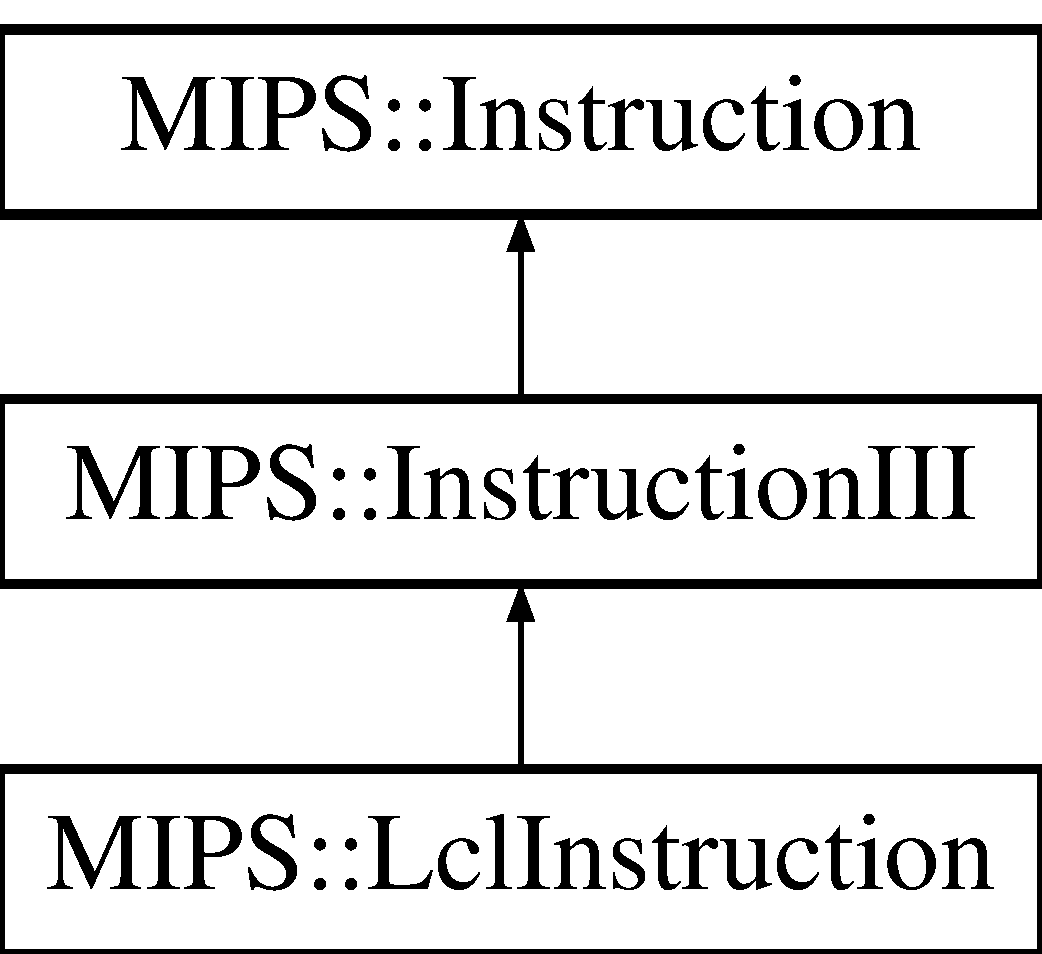
\includegraphics[height=3.000000cm]{classMIPS_1_1LclInstruction}
\end{center}
\end{figure}
\subsection*{Public Member Functions}
\begin{DoxyCompactItemize}
\item 
\hyperlink{classMIPS_1_1LclInstruction_aae1096406aaf2cbf94f7755d05869d05}{Lcl\+Instruction} (\hyperlink{core_8hpp_a6074bae122ae7b527864eec42c728c3c}{bit8\+\_\+t} \hyperlink{classMIPS_1_1Instruction_a45cc6808b5dde8a5d41067d148b55476}{opcode}, \hyperlink{classMIPS_1_1Register}{Register} $\ast$\hyperlink{classMIPS_1_1InstructionIII_a76e7b218fc57cd2fc559bf72498090b6}{rd}, \hyperlink{core_8hpp_a6074bae122ae7b527864eec42c728c3c}{bit8\+\_\+t} \hyperlink{classMIPS_1_1InstructionIII_ad0ebd3b6e7594fc583e9a409bf99a6c7}{offset})
\item 
\hyperlink{core_8hpp_adc265a970bc35995b5879784bbb3f1b7}{bit16\+\_\+t} \hyperlink{classMIPS_1_1LclInstruction_a713c7c0e33c9df49f677abfd95f363db}{execute} ()
\end{DoxyCompactItemize}
\subsection*{Additional Inherited Members}


\subsection{Detailed Description}
Instrução utilizada para carregar 8 bits e carregá-\/los em um no bit menos significativo do registrador definido pelo programador.

\begin{DoxyAuthor}{Author}
Matheus Nogueira 
\end{DoxyAuthor}


\subsection{Constructor \& Destructor Documentation}
\index{M\+I\+P\+S\+::\+Lcl\+Instruction@{M\+I\+P\+S\+::\+Lcl\+Instruction}!Lcl\+Instruction@{Lcl\+Instruction}}
\index{Lcl\+Instruction@{Lcl\+Instruction}!M\+I\+P\+S\+::\+Lcl\+Instruction@{M\+I\+P\+S\+::\+Lcl\+Instruction}}
\subsubsection[{\texorpdfstring{Lcl\+Instruction(bit8\+\_\+t opcode, Register $\ast$rd, bit8\+\_\+t offset)}{LclInstruction(bit8_t opcode, Register *rd, bit8_t offset)}}]{\setlength{\rightskip}{0pt plus 5cm}M\+I\+P\+S\+::\+Lcl\+Instruction\+::\+Lcl\+Instruction (
\begin{DoxyParamCaption}
\item[{{\bf bit8\+\_\+t}}]{opcode, }
\item[{{\bf Register} $\ast$}]{rd, }
\item[{{\bf bit8\+\_\+t}}]{offset}
\end{DoxyParamCaption}
)\hspace{0.3cm}{\ttfamily [inline]}}\hypertarget{classMIPS_1_1LclInstruction_aae1096406aaf2cbf94f7755d05869d05}{}\label{classMIPS_1_1LclInstruction_aae1096406aaf2cbf94f7755d05869d05}
Cria uma instrução de lhc.


\begin{DoxyParams}{Parameters}
{\em opcode} & código da operação \\
\hline
{\em rd} & registrador de destino \\
\hline
{\em offset} & offset de 11 bits \\
\hline
\end{DoxyParams}


\subsection{Member Function Documentation}
\index{M\+I\+P\+S\+::\+Lcl\+Instruction@{M\+I\+P\+S\+::\+Lcl\+Instruction}!execute@{execute}}
\index{execute@{execute}!M\+I\+P\+S\+::\+Lcl\+Instruction@{M\+I\+P\+S\+::\+Lcl\+Instruction}}
\subsubsection[{\texorpdfstring{execute()}{execute()}}]{\setlength{\rightskip}{0pt plus 5cm}{\bf bit16\+\_\+t} M\+I\+P\+S\+::\+Lcl\+Instruction\+::execute (
\begin{DoxyParamCaption}
{}
\end{DoxyParamCaption}
)\hspace{0.3cm}{\ttfamily [virtual]}}\hypertarget{classMIPS_1_1LclInstruction_a713c7c0e33c9df49f677abfd95f363db}{}\label{classMIPS_1_1LclInstruction_a713c7c0e33c9df49f677abfd95f363db}
Executa a instrução.

\begin{DoxyReturn}{Returns}
resultado da operação 
\end{DoxyReturn}


Implements \hyperlink{classMIPS_1_1InstructionIII_aee3071c23abc542e55b446abee766c5e}{M\+I\+P\+S\+::\+Instruction\+I\+II}.



The documentation for this class was generated from the following file\+:\begin{DoxyCompactItemize}
\item 
include/mips/instructions/format\+\_\+\+I\+I\+I/lcl.\+hpp\end{DoxyCompactItemize}

\hypertarget{structMIPS_1_1EventDispatcher_1_1ListenerMap}{}\section{M\+I\+PS\+:\+:Event\+Dispatcher\+:\+:Listener\+Map Struct Reference}
\label{structMIPS_1_1EventDispatcher_1_1ListenerMap}\index{M\+I\+P\+S\+::\+Event\+Dispatcher\+::\+Listener\+Map@{M\+I\+P\+S\+::\+Event\+Dispatcher\+::\+Listener\+Map}}


{\ttfamily \#include $<$event\+\_\+dispatcher.\+hpp$>$}

\subsection*{Public Attributes}
\begin{DoxyCompactItemize}
\item 
\hyperlink{event_8hpp_a2b933d1ba3dc5a595db4dfa5b049c78c}{Event\+Type} \hyperlink{structMIPS_1_1EventDispatcher_1_1ListenerMap_a5ddb37f28dc960baf38ab62d87227cc8}{type}\hypertarget{structMIPS_1_1EventDispatcher_1_1ListenerMap_a5ddb37f28dc960baf38ab62d87227cc8}{}\label{structMIPS_1_1EventDispatcher_1_1ListenerMap_a5ddb37f28dc960baf38ab62d87227cc8}

\begin{DoxyCompactList}\small\item\em Tipo de evento. \end{DoxyCompactList}\item 
\hyperlink{classMIPS_1_1Queue}{Queue}$<$ \hyperlink{classMIPS_1_1EventListener}{Event\+Listener} $\ast$ $>$ $\ast$ \hyperlink{structMIPS_1_1EventDispatcher_1_1ListenerMap_a4cc956ad8c738da563c1db75247e8519}{listeners}\hypertarget{structMIPS_1_1EventDispatcher_1_1ListenerMap_a4cc956ad8c738da563c1db75247e8519}{}\label{structMIPS_1_1EventDispatcher_1_1ListenerMap_a4cc956ad8c738da563c1db75247e8519}

\begin{DoxyCompactList}\small\item\em Fila de ouvintes. \end{DoxyCompactList}\end{DoxyCompactItemize}


\subsection{Detailed Description}
Classe responsável por representar um tipo de evento ligado a uma fila de ouvintes que devem ser notificados. 

The documentation for this struct was generated from the following file\+:\begin{DoxyCompactItemize}
\item 
include/mips/util/event/\hyperlink{event__dispatcher_8hpp}{event\+\_\+dispatcher.\+hpp}\end{DoxyCompactItemize}

\hypertarget{classMIPS_1_1LoadInstruction}{}\section{M\+I\+PS\+:\+:Load\+Instruction Class Reference}
\label{classMIPS_1_1LoadInstruction}\index{M\+I\+P\+S\+::\+Load\+Instruction@{M\+I\+P\+S\+::\+Load\+Instruction}}


{\ttfamily \#include $<$load.\+hpp$>$}

Inheritance diagram for M\+I\+PS\+:\+:Load\+Instruction\+:\begin{figure}[H]
\begin{center}
\leavevmode
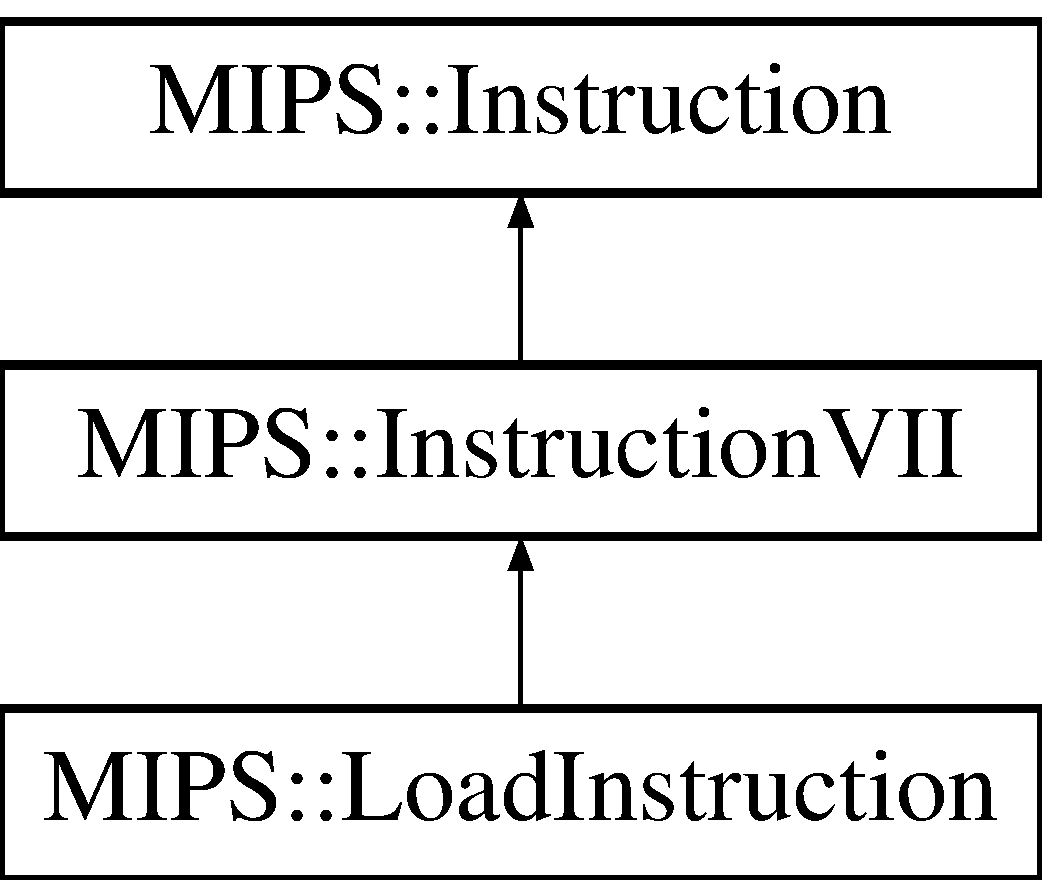
\includegraphics[height=3.000000cm]{classMIPS_1_1LoadInstruction}
\end{center}
\end{figure}
\subsection*{Public Member Functions}
\begin{DoxyCompactItemize}
\item 
\hyperlink{classMIPS_1_1LoadInstruction_a7b21d86c1141e18a8303071dfad8ef0a}{Load\+Instruction} (\hyperlink{core_8hpp_a6074bae122ae7b527864eec42c728c3c}{bit8\+\_\+t} \hyperlink{classMIPS_1_1Instruction_a45cc6808b5dde8a5d41067d148b55476}{opcode}, \hyperlink{classMIPS_1_1Register}{Register} $\ast$\hyperlink{classMIPS_1_1InstructionVII_a8e51202e0b22f8e74668f6de95089e60}{rs}, \hyperlink{classMIPS_1_1Register}{Register} $\ast$\hyperlink{classMIPS_1_1InstructionVII_a8710c06b6e7816f330b0c5daea3402a4}{rt}, \hyperlink{classMIPS_1_1Memory}{Memory} $\ast$\hyperlink{classMIPS_1_1InstructionVII_a4fb34750bedbf137b43f9b55b591e0d7}{memory})
\item 
\hyperlink{core_8hpp_adc265a970bc35995b5879784bbb3f1b7}{bit16\+\_\+t} \hyperlink{classMIPS_1_1LoadInstruction_a847fca19fc0b6ea11ddfda930ac3c749}{execute} ()
\item 
void \hyperlink{classMIPS_1_1LoadInstruction_ae3c3bb9306b797e661fbd778767f577d}{update\+Control} (\hyperlink{classMIPS_1_1ControlUnit}{Control\+Unit} \&control)
\end{DoxyCompactItemize}
\subsection*{Additional Inherited Members}


\subsection{Detailed Description}
Instrução de Load, carrega no registrador C o conteúdo da memória endereçada pelo registrador A.

\begin{DoxyAuthor}{Author}
Felipe Dias 
\end{DoxyAuthor}


\subsection{Constructor \& Destructor Documentation}
\index{M\+I\+P\+S\+::\+Load\+Instruction@{M\+I\+P\+S\+::\+Load\+Instruction}!Load\+Instruction@{Load\+Instruction}}
\index{Load\+Instruction@{Load\+Instruction}!M\+I\+P\+S\+::\+Load\+Instruction@{M\+I\+P\+S\+::\+Load\+Instruction}}
\subsubsection[{\texorpdfstring{Load\+Instruction(bit8\+\_\+t opcode, Register $\ast$rs, Register $\ast$rt, Memory $\ast$memory)}{LoadInstruction(bit8_t opcode, Register *rs, Register *rt, Memory *memory)}}]{\setlength{\rightskip}{0pt plus 5cm}M\+I\+P\+S\+::\+Load\+Instruction\+::\+Load\+Instruction (
\begin{DoxyParamCaption}
\item[{{\bf bit8\+\_\+t}}]{opcode, }
\item[{{\bf Register} $\ast$}]{rs, }
\item[{{\bf Register} $\ast$}]{rt, }
\item[{{\bf Memory} $\ast$}]{memory}
\end{DoxyParamCaption}
)\hspace{0.3cm}{\ttfamily [inline]}}\hypertarget{classMIPS_1_1LoadInstruction_a7b21d86c1141e18a8303071dfad8ef0a}{}\label{classMIPS_1_1LoadInstruction_a7b21d86c1141e18a8303071dfad8ef0a}
Constroi uma nova instrução. 

\subsection{Member Function Documentation}
\index{M\+I\+P\+S\+::\+Load\+Instruction@{M\+I\+P\+S\+::\+Load\+Instruction}!execute@{execute}}
\index{execute@{execute}!M\+I\+P\+S\+::\+Load\+Instruction@{M\+I\+P\+S\+::\+Load\+Instruction}}
\subsubsection[{\texorpdfstring{execute()}{execute()}}]{\setlength{\rightskip}{0pt plus 5cm}{\bf bit16\+\_\+t} M\+I\+P\+S\+::\+Load\+Instruction\+::execute (
\begin{DoxyParamCaption}
{}
\end{DoxyParamCaption}
)\hspace{0.3cm}{\ttfamily [virtual]}}\hypertarget{classMIPS_1_1LoadInstruction_a847fca19fc0b6ea11ddfda930ac3c749}{}\label{classMIPS_1_1LoadInstruction_a847fca19fc0b6ea11ddfda930ac3c749}
Executa a instrução.

\begin{DoxyReturn}{Returns}
resultado da instrução 
\end{DoxyReturn}


Implements \hyperlink{classMIPS_1_1InstructionVII_ab004a9cdc0efa7afacb964352abf3ee7}{M\+I\+P\+S\+::\+Instruction\+V\+II}.

\index{M\+I\+P\+S\+::\+Load\+Instruction@{M\+I\+P\+S\+::\+Load\+Instruction}!update\+Control@{update\+Control}}
\index{update\+Control@{update\+Control}!M\+I\+P\+S\+::\+Load\+Instruction@{M\+I\+P\+S\+::\+Load\+Instruction}}
\subsubsection[{\texorpdfstring{update\+Control(\+Control\+Unit \&control)}{updateControl(ControlUnit &control)}}]{\setlength{\rightskip}{0pt plus 5cm}void M\+I\+P\+S\+::\+Load\+Instruction\+::update\+Control (
\begin{DoxyParamCaption}
\item[{{\bf Control\+Unit} \&}]{control}
\end{DoxyParamCaption}
)\hspace{0.3cm}{\ttfamily [inline]}, {\ttfamily [virtual]}}\hypertarget{classMIPS_1_1LoadInstruction_ae3c3bb9306b797e661fbd778767f577d}{}\label{classMIPS_1_1LoadInstruction_ae3c3bb9306b797e661fbd778767f577d}
Método utilizado para atualizar os sinais de controle do processador.


\begin{DoxyParams}{Parameters}
{\em control} & unidade de controle do processador. \\
\hline
\end{DoxyParams}


Reimplemented from \hyperlink{classMIPS_1_1Instruction_a7df847adef2997446ffca9b71c2f3112}{M\+I\+P\+S\+::\+Instruction}.



The documentation for this class was generated from the following file\+:\begin{DoxyCompactItemize}
\item 
include/mips/instructions/format\+\_\+\+V\+I\+I/\hyperlink{load_8hpp}{load.\+hpp}\end{DoxyCompactItemize}

\hypertarget{classMIPS_1_1LoadlitInstruction}{}\section{M\+I\+PS\+:\+:Loadlit\+Instruction Class Reference}
\label{classMIPS_1_1LoadlitInstruction}\index{M\+I\+P\+S\+::\+Loadlit\+Instruction@{M\+I\+P\+S\+::\+Loadlit\+Instruction}}


{\ttfamily \#include $<$loadlit.\+hpp$>$}

Inheritance diagram for M\+I\+PS\+:\+:Loadlit\+Instruction\+:\begin{figure}[H]
\begin{center}
\leavevmode
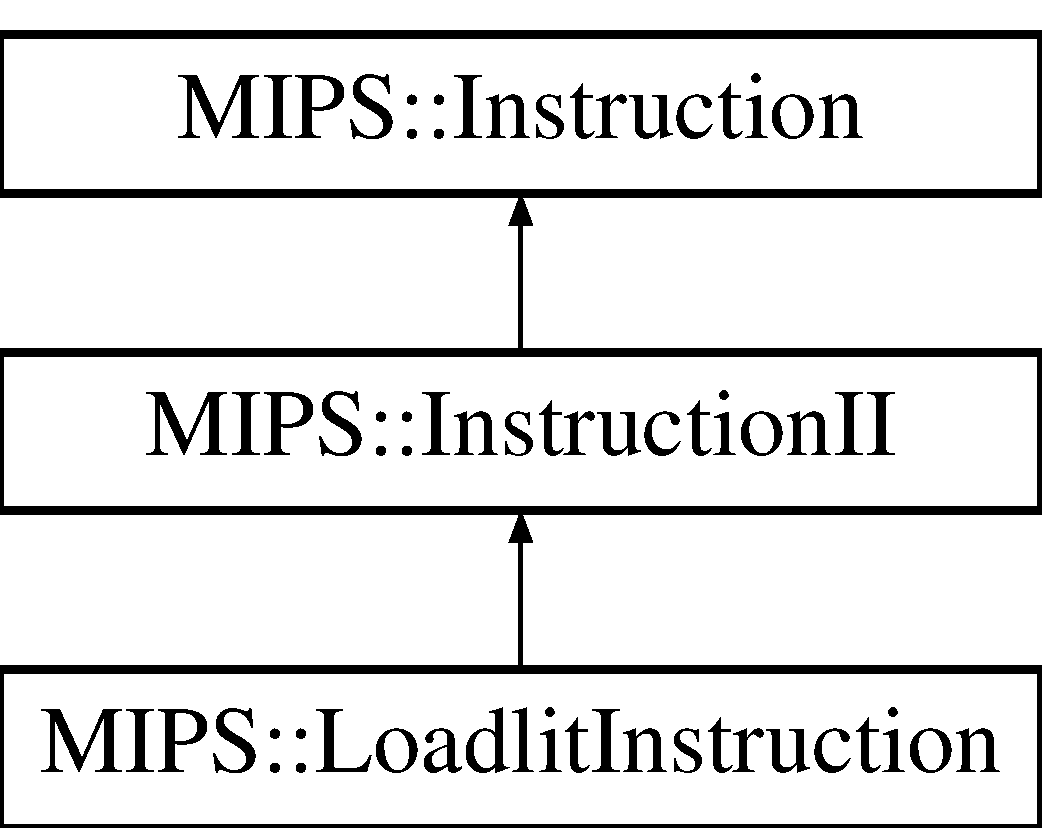
\includegraphics[height=3.000000cm]{classMIPS_1_1LoadlitInstruction}
\end{center}
\end{figure}
\subsection*{Public Member Functions}
\begin{DoxyCompactItemize}
\item 
\hyperlink{classMIPS_1_1LoadlitInstruction_a3f6cbb32be8166dcd9996fcd746ca96d}{Loadlit\+Instruction} (\hyperlink{core_8hpp_a6074bae122ae7b527864eec42c728c3c}{bit8\+\_\+t} \hyperlink{classMIPS_1_1Instruction_a45cc6808b5dde8a5d41067d148b55476}{opcode}, \hyperlink{classMIPS_1_1Register}{Register} $\ast$\hyperlink{classMIPS_1_1InstructionII_a2a709b8170f2bf653de2102df9403e1f}{rd}, \hyperlink{core_8hpp_adc265a970bc35995b5879784bbb3f1b7}{bit16\+\_\+t} \hyperlink{classMIPS_1_1InstructionII_ae34cdcf18cd37944dfecb96d5b07b5cb}{offset})
\item 
\hyperlink{core_8hpp_adc265a970bc35995b5879784bbb3f1b7}{bit16\+\_\+t} \hyperlink{classMIPS_1_1LoadlitInstruction_a9f88a932bbbf31375da7686b449608e1}{execute} ()
\end{DoxyCompactItemize}
\subsection*{Additional Inherited Members}


\subsection{Detailed Description}
Instrução utilizada para carregar 11 bits e carregá-\/los em um registrador definido pelo programador.

\begin{DoxyAuthor}{Author}
Matheus Nogueira 
\end{DoxyAuthor}


\subsection{Constructor \& Destructor Documentation}
\index{M\+I\+P\+S\+::\+Loadlit\+Instruction@{M\+I\+P\+S\+::\+Loadlit\+Instruction}!Loadlit\+Instruction@{Loadlit\+Instruction}}
\index{Loadlit\+Instruction@{Loadlit\+Instruction}!M\+I\+P\+S\+::\+Loadlit\+Instruction@{M\+I\+P\+S\+::\+Loadlit\+Instruction}}
\subsubsection[{\texorpdfstring{Loadlit\+Instruction(bit8\+\_\+t opcode, Register $\ast$rd, bit16\+\_\+t offset)}{LoadlitInstruction(bit8_t opcode, Register *rd, bit16_t offset)}}]{\setlength{\rightskip}{0pt plus 5cm}M\+I\+P\+S\+::\+Loadlit\+Instruction\+::\+Loadlit\+Instruction (
\begin{DoxyParamCaption}
\item[{{\bf bit8\+\_\+t}}]{opcode, }
\item[{{\bf Register} $\ast$}]{rd, }
\item[{{\bf bit16\+\_\+t}}]{offset}
\end{DoxyParamCaption}
)\hspace{0.3cm}{\ttfamily [inline]}}\hypertarget{classMIPS_1_1LoadlitInstruction_a3f6cbb32be8166dcd9996fcd746ca96d}{}\label{classMIPS_1_1LoadlitInstruction_a3f6cbb32be8166dcd9996fcd746ca96d}
Cria uma instrução de loadlit.


\begin{DoxyParams}{Parameters}
{\em opcode} & código da operação \\
\hline
{\em rd} & registrador de destino \\
\hline
{\em offset} & offset de 11 bits \\
\hline
\end{DoxyParams}


\subsection{Member Function Documentation}
\index{M\+I\+P\+S\+::\+Loadlit\+Instruction@{M\+I\+P\+S\+::\+Loadlit\+Instruction}!execute@{execute}}
\index{execute@{execute}!M\+I\+P\+S\+::\+Loadlit\+Instruction@{M\+I\+P\+S\+::\+Loadlit\+Instruction}}
\subsubsection[{\texorpdfstring{execute()}{execute()}}]{\setlength{\rightskip}{0pt plus 5cm}{\bf bit16\+\_\+t} M\+I\+P\+S\+::\+Loadlit\+Instruction\+::execute (
\begin{DoxyParamCaption}
{}
\end{DoxyParamCaption}
)\hspace{0.3cm}{\ttfamily [virtual]}}\hypertarget{classMIPS_1_1LoadlitInstruction_a9f88a932bbbf31375da7686b449608e1}{}\label{classMIPS_1_1LoadlitInstruction_a9f88a932bbbf31375da7686b449608e1}
Executa a instrução.

\begin{DoxyReturn}{Returns}
resultado da operação 
\end{DoxyReturn}


Implements \hyperlink{classMIPS_1_1InstructionII_aa014c5b0fe877746ca4db85c971a2e93}{M\+I\+P\+S\+::\+Instruction\+II}.



The documentation for this class was generated from the following file\+:\begin{DoxyCompactItemize}
\item 
include/mips/instructions/format\+\_\+\+I\+I/\hyperlink{loadlit_8hpp}{loadlit.\+hpp}\end{DoxyCompactItemize}

\hypertarget{classMIPS_1_1LslInstruction}{}\section{M\+I\+PS\+:\+:Lsl\+Instruction Class Reference}
\label{classMIPS_1_1LslInstruction}\index{M\+I\+P\+S\+::\+Lsl\+Instruction@{M\+I\+P\+S\+::\+Lsl\+Instruction}}


{\ttfamily \#include $<$lsl.\+hpp$>$}

Inheritance diagram for M\+I\+PS\+:\+:Lsl\+Instruction\+:\begin{figure}[H]
\begin{center}
\leavevmode
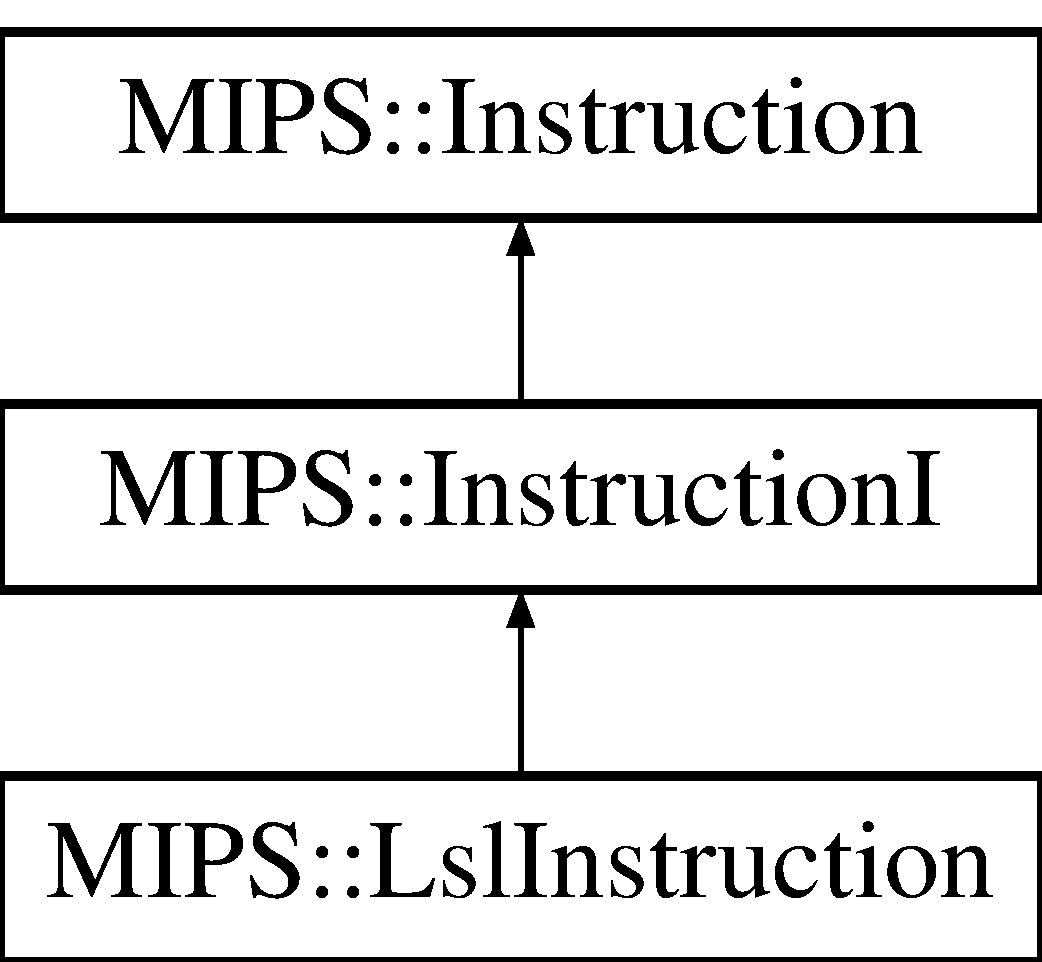
\includegraphics[height=3.000000cm]{classMIPS_1_1LslInstruction}
\end{center}
\end{figure}
\subsection*{Public Member Functions}
\begin{DoxyCompactItemize}
\item 
\hyperlink{classMIPS_1_1LslInstruction_ae6e4596399372f3eb4eb4b9685e107e6}{Lsl\+Instruction} (\hyperlink{core_8hpp_a6074bae122ae7b527864eec42c728c3c}{bit8\+\_\+t} \hyperlink{classMIPS_1_1Instruction_a45cc6808b5dde8a5d41067d148b55476}{opcode}, \hyperlink{classMIPS_1_1Register}{Register} $\ast$\hyperlink{classMIPS_1_1InstructionI_a2be191d5b3dce505e2e626ec02eb4d62}{rs}, \hyperlink{classMIPS_1_1Register}{Register} $\ast$\hyperlink{classMIPS_1_1InstructionI_add1db07a5c954f35271de8c8a5737487}{rt}, \hyperlink{core_8hpp_a6074bae122ae7b527864eec42c728c3c}{bit8\+\_\+t} \hyperlink{classMIPS_1_1InstructionI_aa9b6da37c374c2ec8d96448d341e5e7d}{shamt}, \hyperlink{core_8hpp_a6074bae122ae7b527864eec42c728c3c}{bit8\+\_\+t} \hyperlink{classMIPS_1_1InstructionI_a5c6efcbbd233a7447c1fe24ea0a1e558}{funct})
\item 
\hyperlink{core_8hpp_adc265a970bc35995b5879784bbb3f1b7}{bit16\+\_\+t} \hyperlink{classMIPS_1_1LslInstruction_af6483e18e765310b9900c7fd8322b0c8}{execute} ()
\end{DoxyCompactItemize}
\subsection*{Additional Inherited Members}


\subsection{Detailed Description}
Classe que faz a operação de L\+SL no processador.

\begin{DoxyAuthor}{Author}
Felipe Dias 
\end{DoxyAuthor}


\subsection{Constructor \& Destructor Documentation}
\index{M\+I\+P\+S\+::\+Lsl\+Instruction@{M\+I\+P\+S\+::\+Lsl\+Instruction}!Lsl\+Instruction@{Lsl\+Instruction}}
\index{Lsl\+Instruction@{Lsl\+Instruction}!M\+I\+P\+S\+::\+Lsl\+Instruction@{M\+I\+P\+S\+::\+Lsl\+Instruction}}
\subsubsection[{\texorpdfstring{Lsl\+Instruction(bit8\+\_\+t opcode, Register $\ast$rs, Register $\ast$rt, bit8\+\_\+t shamt, bit8\+\_\+t funct)}{LslInstruction(bit8_t opcode, Register *rs, Register *rt, bit8_t shamt, bit8_t funct)}}]{\setlength{\rightskip}{0pt plus 5cm}M\+I\+P\+S\+::\+Lsl\+Instruction\+::\+Lsl\+Instruction (
\begin{DoxyParamCaption}
\item[{{\bf bit8\+\_\+t}}]{opcode, }
\item[{{\bf Register} $\ast$}]{rs, }
\item[{{\bf Register} $\ast$}]{rt, }
\item[{{\bf bit8\+\_\+t}}]{shamt, }
\item[{{\bf bit8\+\_\+t}}]{funct}
\end{DoxyParamCaption}
)\hspace{0.3cm}{\ttfamily [inline]}}\hypertarget{classMIPS_1_1LslInstruction_ae6e4596399372f3eb4eb4b9685e107e6}{}\label{classMIPS_1_1LslInstruction_ae6e4596399372f3eb4eb4b9685e107e6}
Constroi uma nova instrução. 

\subsection{Member Function Documentation}
\index{M\+I\+P\+S\+::\+Lsl\+Instruction@{M\+I\+P\+S\+::\+Lsl\+Instruction}!execute@{execute}}
\index{execute@{execute}!M\+I\+P\+S\+::\+Lsl\+Instruction@{M\+I\+P\+S\+::\+Lsl\+Instruction}}
\subsubsection[{\texorpdfstring{execute()}{execute()}}]{\setlength{\rightskip}{0pt plus 5cm}{\bf bit16\+\_\+t} M\+I\+P\+S\+::\+Lsl\+Instruction\+::execute (
\begin{DoxyParamCaption}
{}
\end{DoxyParamCaption}
)\hspace{0.3cm}{\ttfamily [virtual]}}\hypertarget{classMIPS_1_1LslInstruction_af6483e18e765310b9900c7fd8322b0c8}{}\label{classMIPS_1_1LslInstruction_af6483e18e765310b9900c7fd8322b0c8}
Função que executa a operação de decremento.

\begin{DoxyReturn}{Returns}
resultado da operação 
\end{DoxyReturn}


Implements \hyperlink{classMIPS_1_1InstructionI_ae60fca5801bf5415cdff06d2aa11764f}{M\+I\+P\+S\+::\+InstructionI}.



The documentation for this class was generated from the following file\+:\begin{DoxyCompactItemize}
\item 
include/mips/instructions/format\+\_\+\+I/\hyperlink{lsl_8hpp}{lsl.\+hpp}\end{DoxyCompactItemize}

\hypertarget{classMIPS_1_1LsrInstruction}{}\section{M\+I\+PS\+:\+:Lsr\+Instruction Class Reference}
\label{classMIPS_1_1LsrInstruction}\index{M\+I\+P\+S\+::\+Lsr\+Instruction@{M\+I\+P\+S\+::\+Lsr\+Instruction}}


{\ttfamily \#include $<$lsr.\+hpp$>$}

Inheritance diagram for M\+I\+PS\+:\+:Lsr\+Instruction\+:\begin{figure}[H]
\begin{center}
\leavevmode
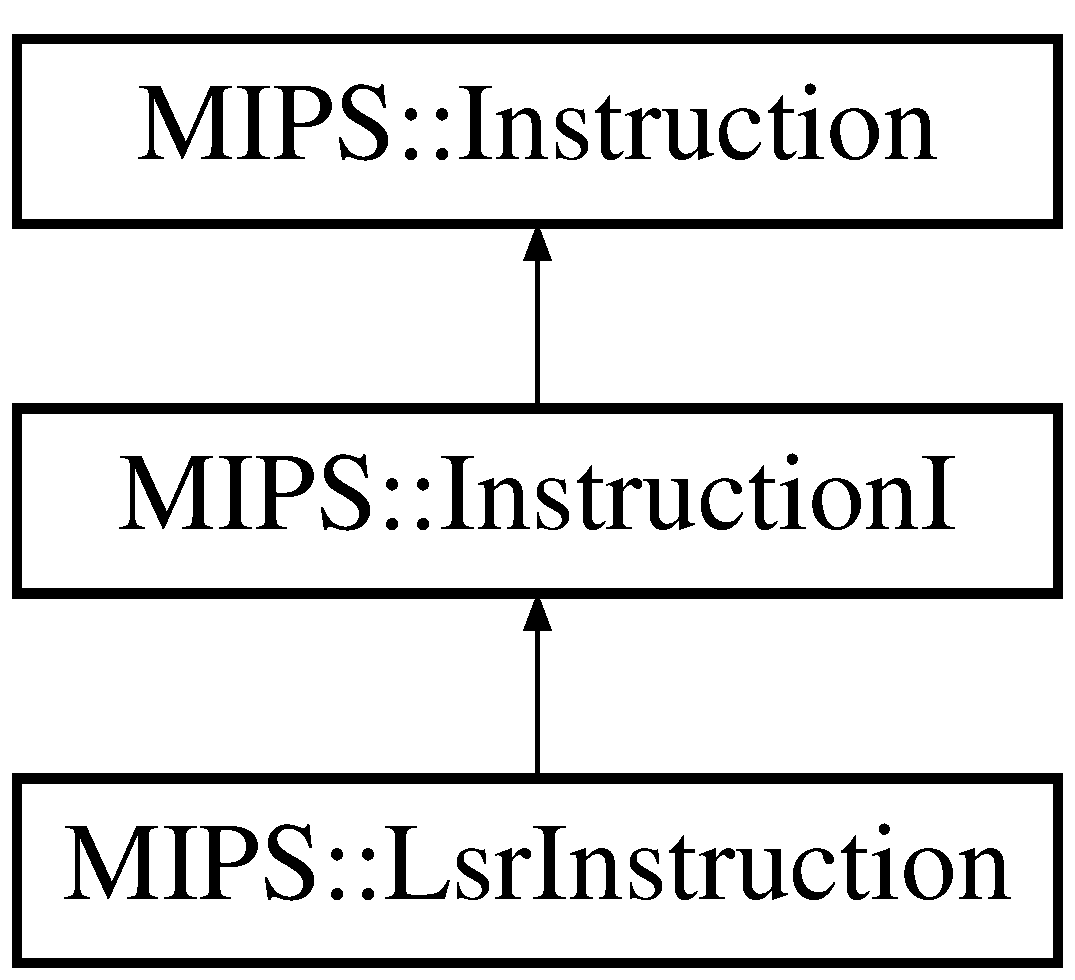
\includegraphics[height=3.000000cm]{classMIPS_1_1LsrInstruction}
\end{center}
\end{figure}
\subsection*{Public Member Functions}
\begin{DoxyCompactItemize}
\item 
\hyperlink{classMIPS_1_1LsrInstruction_a20419b31090528cc13610dd7399f511c}{Lsr\+Instruction} (\hyperlink{core_8hpp_a6074bae122ae7b527864eec42c728c3c}{bit8\+\_\+t} \hyperlink{classMIPS_1_1Instruction_a45cc6808b5dde8a5d41067d148b55476}{opcode}, \hyperlink{classMIPS_1_1Register}{Register} $\ast$\hyperlink{classMIPS_1_1InstructionI_a2be191d5b3dce505e2e626ec02eb4d62}{rs}, \hyperlink{classMIPS_1_1Register}{Register} $\ast$\hyperlink{classMIPS_1_1InstructionI_add1db07a5c954f35271de8c8a5737487}{rt}, \hyperlink{core_8hpp_a6074bae122ae7b527864eec42c728c3c}{bit8\+\_\+t} \hyperlink{classMIPS_1_1InstructionI_aa9b6da37c374c2ec8d96448d341e5e7d}{shamt}, \hyperlink{core_8hpp_a6074bae122ae7b527864eec42c728c3c}{bit8\+\_\+t} \hyperlink{classMIPS_1_1InstructionI_a5c6efcbbd233a7447c1fe24ea0a1e558}{funct})
\item 
\hyperlink{core_8hpp_adc265a970bc35995b5879784bbb3f1b7}{bit16\+\_\+t} \hyperlink{classMIPS_1_1LsrInstruction_ae4417a1e7d66faec1361f8884f69c9b2}{execute} ()
\end{DoxyCompactItemize}
\subsection*{Additional Inherited Members}


\subsection{Detailed Description}
Classe que faz a operação de L\+SR no processador.

\begin{DoxyAuthor}{Author}
Felipe Dias 
\end{DoxyAuthor}


\subsection{Constructor \& Destructor Documentation}
\index{M\+I\+P\+S\+::\+Lsr\+Instruction@{M\+I\+P\+S\+::\+Lsr\+Instruction}!Lsr\+Instruction@{Lsr\+Instruction}}
\index{Lsr\+Instruction@{Lsr\+Instruction}!M\+I\+P\+S\+::\+Lsr\+Instruction@{M\+I\+P\+S\+::\+Lsr\+Instruction}}
\subsubsection[{\texorpdfstring{Lsr\+Instruction(bit8\+\_\+t opcode, Register $\ast$rs, Register $\ast$rt, bit8\+\_\+t shamt, bit8\+\_\+t funct)}{LsrInstruction(bit8_t opcode, Register *rs, Register *rt, bit8_t shamt, bit8_t funct)}}]{\setlength{\rightskip}{0pt plus 5cm}M\+I\+P\+S\+::\+Lsr\+Instruction\+::\+Lsr\+Instruction (
\begin{DoxyParamCaption}
\item[{{\bf bit8\+\_\+t}}]{opcode, }
\item[{{\bf Register} $\ast$}]{rs, }
\item[{{\bf Register} $\ast$}]{rt, }
\item[{{\bf bit8\+\_\+t}}]{shamt, }
\item[{{\bf bit8\+\_\+t}}]{funct}
\end{DoxyParamCaption}
)\hspace{0.3cm}{\ttfamily [inline]}}\hypertarget{classMIPS_1_1LsrInstruction_a20419b31090528cc13610dd7399f511c}{}\label{classMIPS_1_1LsrInstruction_a20419b31090528cc13610dd7399f511c}
Constroi uma nova instrução. 

\subsection{Member Function Documentation}
\index{M\+I\+P\+S\+::\+Lsr\+Instruction@{M\+I\+P\+S\+::\+Lsr\+Instruction}!execute@{execute}}
\index{execute@{execute}!M\+I\+P\+S\+::\+Lsr\+Instruction@{M\+I\+P\+S\+::\+Lsr\+Instruction}}
\subsubsection[{\texorpdfstring{execute()}{execute()}}]{\setlength{\rightskip}{0pt plus 5cm}{\bf bit16\+\_\+t} M\+I\+P\+S\+::\+Lsr\+Instruction\+::execute (
\begin{DoxyParamCaption}
{}
\end{DoxyParamCaption}
)\hspace{0.3cm}{\ttfamily [virtual]}}\hypertarget{classMIPS_1_1LsrInstruction_ae4417a1e7d66faec1361f8884f69c9b2}{}\label{classMIPS_1_1LsrInstruction_ae4417a1e7d66faec1361f8884f69c9b2}
Função que executa a operação de decremento.

\begin{DoxyReturn}{Returns}
resultado da operação 
\end{DoxyReturn}


Implements \hyperlink{classMIPS_1_1InstructionI_ae60fca5801bf5415cdff06d2aa11764f}{M\+I\+P\+S\+::\+InstructionI}.



The documentation for this class was generated from the following file\+:\begin{DoxyCompactItemize}
\item 
include/mips/instructions/format\+\_\+\+I/\hyperlink{lsr_8hpp}{lsr.\+hpp}\end{DoxyCompactItemize}

\hypertarget{classMIPS_1_1Memory}{}\section{M\+I\+PS\+:\+:Memory Class Reference}
\label{classMIPS_1_1Memory}\index{M\+I\+P\+S\+::\+Memory@{M\+I\+P\+S\+::\+Memory}}


{\ttfamily \#include $<$memory.\+hpp$>$}

\subsection*{Public Member Functions}
\begin{DoxyCompactItemize}
\item 
\hyperlink{classMIPS_1_1Memory_a092aefef9b57b4a349fb11a780f1cc5a}{Memory} (\hyperlink{classMIPS_1_1ControlUnit}{Control\+Unit} \&control\+Unit)
\item 
\hyperlink{classMIPS_1_1Memory_ace3e886fa42efa3e629c7572bf232e05}{$\sim$\+Memory} ()
\item 
void \hyperlink{classMIPS_1_1Memory_a636e0ca3d23fc5022a2a4b59a6648210}{set\+Instruction\+Size} (size\+\_\+t size)
\item 
void \hyperlink{classMIPS_1_1Memory_a53b03b417ee8efb4a6f3a0020c3bd7ab}{set\+Data\+Size} (size\+\_\+t size)
\item 
void \hyperlink{classMIPS_1_1Memory_a8d339b30f29c4dc8044b51c982d5e95b}{write} (\hyperlink{core_8hpp_adc265a970bc35995b5879784bbb3f1b7}{bit16\+\_\+t} data, \hyperlink{core_8hpp_ad5f4c6ca614f67be232930e0e31b9ccc}{bit32\+\_\+t} offset, \hyperlink{core_8hpp_a6074bae122ae7b527864eec42c728c3c}{bit8\+\_\+t} i\+OrD=1)
\item 
\hyperlink{core_8hpp_adc265a970bc35995b5879784bbb3f1b7}{bit16\+\_\+t} \hyperlink{classMIPS_1_1Memory_a93a2aecd6026ecd86e77fcef6b99b91b}{read} (\hyperlink{core_8hpp_ad5f4c6ca614f67be232930e0e31b9ccc}{bit32\+\_\+t} offset, \hyperlink{core_8hpp_a6074bae122ae7b527864eec42c728c3c}{bit8\+\_\+t} i\+OrD=1)
\end{DoxyCompactItemize}


\subsection{Detailed Description}
Classe responsável por iteragir com a memória do processador, para assim, criar uma interface de maior facilidade para acessar a memória.

\begin{DoxyAuthor}{Author}
Matheus Nogueira 
\end{DoxyAuthor}


\subsection{Constructor \& Destructor Documentation}
\index{M\+I\+P\+S\+::\+Memory@{M\+I\+P\+S\+::\+Memory}!Memory@{Memory}}
\index{Memory@{Memory}!M\+I\+P\+S\+::\+Memory@{M\+I\+P\+S\+::\+Memory}}
\subsubsection[{\texorpdfstring{Memory(\+Control\+Unit \&control\+Unit)}{Memory(ControlUnit &controlUnit)}}]{\setlength{\rightskip}{0pt plus 5cm}M\+I\+P\+S\+::\+Memory\+::\+Memory (
\begin{DoxyParamCaption}
\item[{{\bf Control\+Unit} \&}]{control\+Unit}
\end{DoxyParamCaption}
)}\hypertarget{classMIPS_1_1Memory_a092aefef9b57b4a349fb11a780f1cc5a}{}\label{classMIPS_1_1Memory_a092aefef9b57b4a349fb11a780f1cc5a}
Cria uma nova unidade de memória.


\begin{DoxyParams}{Parameters}
{\em control\+Unit} & unidade de controle do processador. \\
\hline
\end{DoxyParams}
\index{M\+I\+P\+S\+::\+Memory@{M\+I\+P\+S\+::\+Memory}!````~Memory@{$\sim$\+Memory}}
\index{````~Memory@{$\sim$\+Memory}!M\+I\+P\+S\+::\+Memory@{M\+I\+P\+S\+::\+Memory}}
\subsubsection[{\texorpdfstring{$\sim$\+Memory()}{~Memory()}}]{\setlength{\rightskip}{0pt plus 5cm}M\+I\+P\+S\+::\+Memory\+::$\sim$\+Memory (
\begin{DoxyParamCaption}
{}
\end{DoxyParamCaption}
)}\hypertarget{classMIPS_1_1Memory_ace3e886fa42efa3e629c7572bf232e05}{}\label{classMIPS_1_1Memory_ace3e886fa42efa3e629c7572bf232e05}
Destroi a unidade de memória. 

\subsection{Member Function Documentation}
\index{M\+I\+P\+S\+::\+Memory@{M\+I\+P\+S\+::\+Memory}!read@{read}}
\index{read@{read}!M\+I\+P\+S\+::\+Memory@{M\+I\+P\+S\+::\+Memory}}
\subsubsection[{\texorpdfstring{read(bit32\+\_\+t offset, bit8\+\_\+t i\+Or\+D=1)}{read(bit32_t offset, bit8_t iOrD=1)}}]{\setlength{\rightskip}{0pt plus 5cm}{\bf bit16\+\_\+t} M\+I\+P\+S\+::\+Memory\+::read (
\begin{DoxyParamCaption}
\item[{{\bf bit32\+\_\+t}}]{offset, }
\item[{{\bf bit8\+\_\+t}}]{i\+OrD = {\ttfamily 1}}
\end{DoxyParamCaption}
)}\hypertarget{classMIPS_1_1Memory_a93a2aecd6026ecd86e77fcef6b99b91b}{}\label{classMIPS_1_1Memory_a93a2aecd6026ecd86e77fcef6b99b91b}
Lẽ uma palavra que está na posição de memória especificada.


\begin{DoxyParams}{Parameters}
{\em offset} & posição da memória que será lida. \\
\hline
{\em i\+OrD} & tipo de dado que será lido (instruçao ou dado) (padrão\+: dado) \\
\hline
\end{DoxyParams}
\begin{DoxyReturn}{Returns}
palavra armazenada na posição de memória especificada. 
\end{DoxyReturn}
\index{M\+I\+P\+S\+::\+Memory@{M\+I\+P\+S\+::\+Memory}!set\+Data\+Size@{set\+Data\+Size}}
\index{set\+Data\+Size@{set\+Data\+Size}!M\+I\+P\+S\+::\+Memory@{M\+I\+P\+S\+::\+Memory}}
\subsubsection[{\texorpdfstring{set\+Data\+Size(size\+\_\+t size)}{setDataSize(size_t size)}}]{\setlength{\rightskip}{0pt plus 5cm}void M\+I\+P\+S\+::\+Memory\+::set\+Data\+Size (
\begin{DoxyParamCaption}
\item[{size\+\_\+t}]{size}
\end{DoxyParamCaption}
)}\hypertarget{classMIPS_1_1Memory_a53b03b417ee8efb4a6f3a0020c3bd7ab}{}\label{classMIPS_1_1Memory_a53b03b417ee8efb4a6f3a0020c3bd7ab}
Define o tamanho da memória de dados.


\begin{DoxyParams}{Parameters}
{\em size} & tamanho da memória em número de palavras. \\
\hline
\end{DoxyParams}
\index{M\+I\+P\+S\+::\+Memory@{M\+I\+P\+S\+::\+Memory}!set\+Instruction\+Size@{set\+Instruction\+Size}}
\index{set\+Instruction\+Size@{set\+Instruction\+Size}!M\+I\+P\+S\+::\+Memory@{M\+I\+P\+S\+::\+Memory}}
\subsubsection[{\texorpdfstring{set\+Instruction\+Size(size\+\_\+t size)}{setInstructionSize(size_t size)}}]{\setlength{\rightskip}{0pt plus 5cm}void M\+I\+P\+S\+::\+Memory\+::set\+Instruction\+Size (
\begin{DoxyParamCaption}
\item[{size\+\_\+t}]{size}
\end{DoxyParamCaption}
)}\hypertarget{classMIPS_1_1Memory_a636e0ca3d23fc5022a2a4b59a6648210}{}\label{classMIPS_1_1Memory_a636e0ca3d23fc5022a2a4b59a6648210}
Define o tamanho da memória de instruções.


\begin{DoxyParams}{Parameters}
{\em size} & tamanho da memória em número de palavras. \\
\hline
\end{DoxyParams}
\index{M\+I\+P\+S\+::\+Memory@{M\+I\+P\+S\+::\+Memory}!write@{write}}
\index{write@{write}!M\+I\+P\+S\+::\+Memory@{M\+I\+P\+S\+::\+Memory}}
\subsubsection[{\texorpdfstring{write(bit16\+\_\+t data, bit32\+\_\+t offset, bit8\+\_\+t i\+Or\+D=1)}{write(bit16_t data, bit32_t offset, bit8_t iOrD=1)}}]{\setlength{\rightskip}{0pt plus 5cm}void M\+I\+P\+S\+::\+Memory\+::write (
\begin{DoxyParamCaption}
\item[{{\bf bit16\+\_\+t}}]{data, }
\item[{{\bf bit32\+\_\+t}}]{offset, }
\item[{{\bf bit8\+\_\+t}}]{i\+OrD = {\ttfamily 1}}
\end{DoxyParamCaption}
)}\hypertarget{classMIPS_1_1Memory_a8d339b30f29c4dc8044b51c982d5e95b}{}\label{classMIPS_1_1Memory_a8d339b30f29c4dc8044b51c982d5e95b}
Escreve uma palavra na posição de memória especificada.


\begin{DoxyParams}{Parameters}
{\em data} & palavra que será escrita. \\
\hline
{\em offset} & posição da memória em que a palavra será escrita. \\
\hline
{\em i\+OrD} & tipo de dado que será escrito (instrução ou dados) (padrão\+: dado) \\
\hline
\end{DoxyParams}


The documentation for this class was generated from the following file\+:\begin{DoxyCompactItemize}
\item 
include/mips/memory/\hyperlink{memory_8hpp}{memory.\+hpp}\end{DoxyCompactItemize}

\hypertarget{classMIPS_1_1MemoryException}{}\section{M\+I\+PS\+:\+:Memory\+Exception Class Reference}
\label{classMIPS_1_1MemoryException}\index{M\+I\+P\+S\+::\+Memory\+Exception@{M\+I\+P\+S\+::\+Memory\+Exception}}


{\ttfamily \#include $<$memory\+\_\+exception.\+hpp$>$}

Inheritance diagram for M\+I\+PS\+:\+:Memory\+Exception\+:\begin{figure}[H]
\begin{center}
\leavevmode
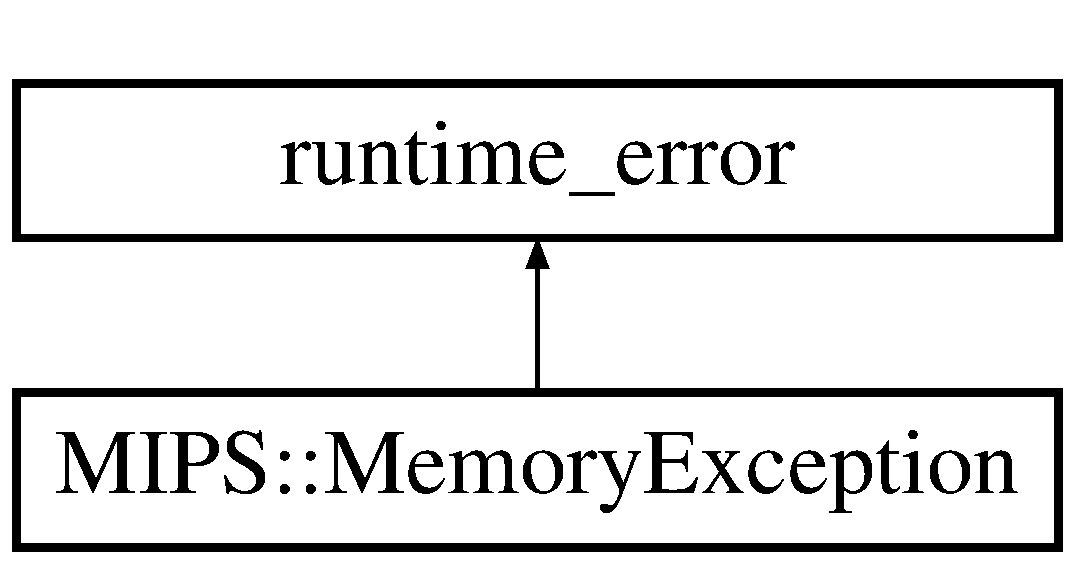
\includegraphics[height=2.000000cm]{classMIPS_1_1MemoryException}
\end{center}
\end{figure}
\subsection*{Public Member Functions}
\begin{DoxyCompactItemize}
\item 
\hyperlink{classMIPS_1_1MemoryException_a71649bc565f55557f59622781de590c7}{Memory\+Exception} (const char $\ast$msg)
\item 
virtual const char $\ast$ \hyperlink{classMIPS_1_1MemoryException_a8ee2a716f1c715577736d7b6694d3672}{what} () const   throw ()
\end{DoxyCompactItemize}


\subsection{Detailed Description}
Exceção que é lançada pelo interpretador quando um erro é encontrado durante o acesso à memória.

\begin{DoxyAuthor}{Author}
Matheus Nogueira 
\end{DoxyAuthor}


\subsection{Constructor \& Destructor Documentation}
\index{M\+I\+P\+S\+::\+Memory\+Exception@{M\+I\+P\+S\+::\+Memory\+Exception}!Memory\+Exception@{Memory\+Exception}}
\index{Memory\+Exception@{Memory\+Exception}!M\+I\+P\+S\+::\+Memory\+Exception@{M\+I\+P\+S\+::\+Memory\+Exception}}
\subsubsection[{\texorpdfstring{Memory\+Exception(const char $\ast$msg)}{MemoryException(const char *msg)}}]{\setlength{\rightskip}{0pt plus 5cm}M\+I\+P\+S\+::\+Memory\+Exception\+::\+Memory\+Exception (
\begin{DoxyParamCaption}
\item[{const char $\ast$}]{msg}
\end{DoxyParamCaption}
)\hspace{0.3cm}{\ttfamily [inline]}}\hypertarget{classMIPS_1_1MemoryException_a71649bc565f55557f59622781de590c7}{}\label{classMIPS_1_1MemoryException_a71649bc565f55557f59622781de590c7}
Cria uma nova exceção.


\begin{DoxyParams}{Parameters}
{\em msg} & mensagem de erro. \\
\hline
\end{DoxyParams}


\subsection{Member Function Documentation}
\index{M\+I\+P\+S\+::\+Memory\+Exception@{M\+I\+P\+S\+::\+Memory\+Exception}!what@{what}}
\index{what@{what}!M\+I\+P\+S\+::\+Memory\+Exception@{M\+I\+P\+S\+::\+Memory\+Exception}}
\subsubsection[{\texorpdfstring{what() const }{what() const }}]{\setlength{\rightskip}{0pt plus 5cm}virtual const char$\ast$ M\+I\+P\+S\+::\+Memory\+Exception\+::what (
\begin{DoxyParamCaption}
{}
\end{DoxyParamCaption}
) const throw  ) \hspace{0.3cm}{\ttfamily [inline]}, {\ttfamily [virtual]}}\hypertarget{classMIPS_1_1MemoryException_a8ee2a716f1c715577736d7b6694d3672}{}\label{classMIPS_1_1MemoryException_a8ee2a716f1c715577736d7b6694d3672}
Retorna a mensagem de erro.

\begin{DoxyReturn}{Returns}
mensagem de erro. 
\end{DoxyReturn}


The documentation for this class was generated from the following file\+:\begin{DoxyCompactItemize}
\item 
include/mips/memory/\hyperlink{memory__exception_8hpp}{memory\+\_\+exception.\+hpp}\end{DoxyCompactItemize}

\hypertarget{classMIPS_1_1NandInstruction}{}\section{M\+I\+PS\+:\+:Nand\+Instruction Class Reference}
\label{classMIPS_1_1NandInstruction}\index{M\+I\+P\+S\+::\+Nand\+Instruction@{M\+I\+P\+S\+::\+Nand\+Instruction}}


{\ttfamily \#include $<$nand.\+hpp$>$}

Inheritance diagram for M\+I\+PS\+:\+:Nand\+Instruction\+:\begin{figure}[H]
\begin{center}
\leavevmode
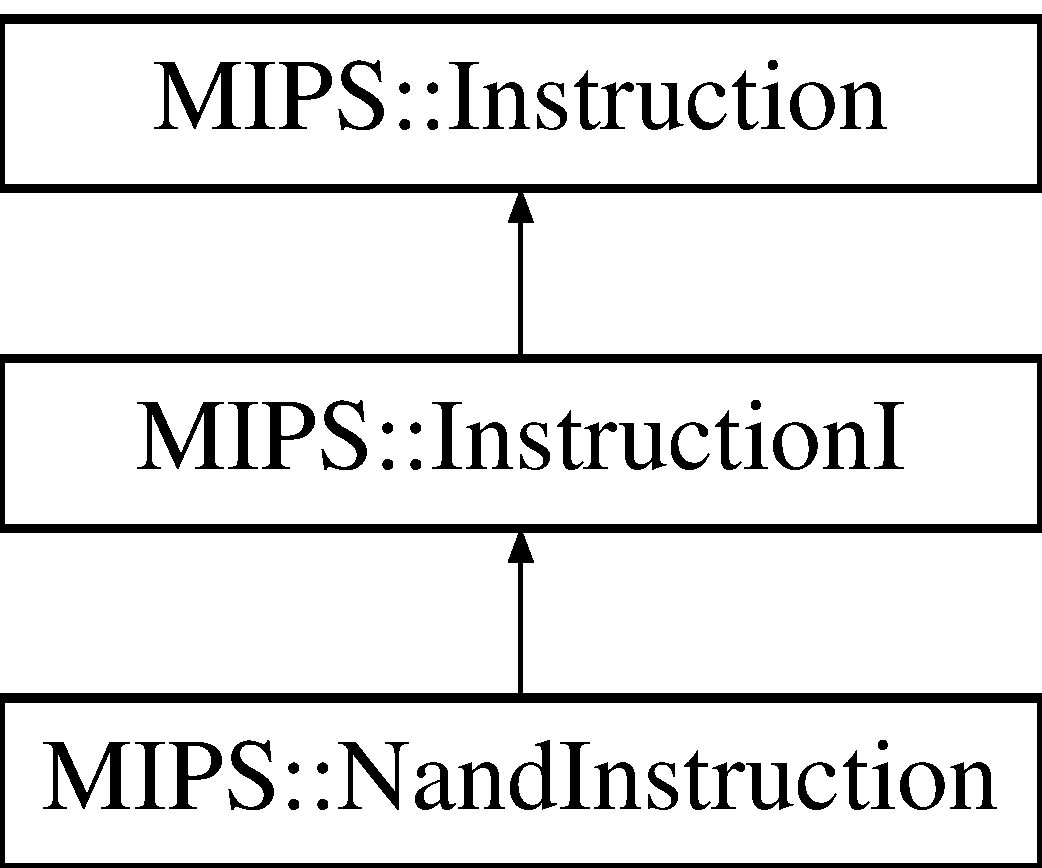
\includegraphics[height=3.000000cm]{classMIPS_1_1NandInstruction}
\end{center}
\end{figure}
\subsection*{Public Member Functions}
\begin{DoxyCompactItemize}
\item 
\hyperlink{classMIPS_1_1NandInstruction_a1c401e26e08324e1ba50175c4a08f4e7}{Nand\+Instruction} (\hyperlink{core_8hpp_a6074bae122ae7b527864eec42c728c3c}{bit8\+\_\+t} \hyperlink{classMIPS_1_1Instruction_a45cc6808b5dde8a5d41067d148b55476}{opcode}, \hyperlink{classMIPS_1_1Register}{Register} $\ast$\hyperlink{classMIPS_1_1InstructionI_a2be191d5b3dce505e2e626ec02eb4d62}{rs}, \hyperlink{classMIPS_1_1Register}{Register} $\ast$\hyperlink{classMIPS_1_1InstructionI_add1db07a5c954f35271de8c8a5737487}{rt}, \hyperlink{core_8hpp_a6074bae122ae7b527864eec42c728c3c}{bit8\+\_\+t} \hyperlink{classMIPS_1_1InstructionI_aa9b6da37c374c2ec8d96448d341e5e7d}{shamt}, \hyperlink{core_8hpp_a6074bae122ae7b527864eec42c728c3c}{bit8\+\_\+t} \hyperlink{classMIPS_1_1InstructionI_a5c6efcbbd233a7447c1fe24ea0a1e558}{funct})
\item 
\hyperlink{core_8hpp_adc265a970bc35995b5879784bbb3f1b7}{bit16\+\_\+t} \hyperlink{classMIPS_1_1NandInstruction_a2e0266ebee3819e7b4d9bfb44f0e70ac}{execute} ()
\end{DoxyCompactItemize}
\subsection*{Additional Inherited Members}


\subsection{Detailed Description}
Classe que faz a operação de N\+A\+ND no processador.

\begin{DoxyAuthor}{Author}
Matheus Nogueira 
\end{DoxyAuthor}


\subsection{Constructor \& Destructor Documentation}
\index{M\+I\+P\+S\+::\+Nand\+Instruction@{M\+I\+P\+S\+::\+Nand\+Instruction}!Nand\+Instruction@{Nand\+Instruction}}
\index{Nand\+Instruction@{Nand\+Instruction}!M\+I\+P\+S\+::\+Nand\+Instruction@{M\+I\+P\+S\+::\+Nand\+Instruction}}
\subsubsection[{\texorpdfstring{Nand\+Instruction(bit8\+\_\+t opcode, Register $\ast$rs, Register $\ast$rt, bit8\+\_\+t shamt, bit8\+\_\+t funct)}{NandInstruction(bit8_t opcode, Register *rs, Register *rt, bit8_t shamt, bit8_t funct)}}]{\setlength{\rightskip}{0pt plus 5cm}M\+I\+P\+S\+::\+Nand\+Instruction\+::\+Nand\+Instruction (
\begin{DoxyParamCaption}
\item[{{\bf bit8\+\_\+t}}]{opcode, }
\item[{{\bf Register} $\ast$}]{rs, }
\item[{{\bf Register} $\ast$}]{rt, }
\item[{{\bf bit8\+\_\+t}}]{shamt, }
\item[{{\bf bit8\+\_\+t}}]{funct}
\end{DoxyParamCaption}
)\hspace{0.3cm}{\ttfamily [inline]}}\hypertarget{classMIPS_1_1NandInstruction_a1c401e26e08324e1ba50175c4a08f4e7}{}\label{classMIPS_1_1NandInstruction_a1c401e26e08324e1ba50175c4a08f4e7}
Constroi uma nova instrução. 

\subsection{Member Function Documentation}
\index{M\+I\+P\+S\+::\+Nand\+Instruction@{M\+I\+P\+S\+::\+Nand\+Instruction}!execute@{execute}}
\index{execute@{execute}!M\+I\+P\+S\+::\+Nand\+Instruction@{M\+I\+P\+S\+::\+Nand\+Instruction}}
\subsubsection[{\texorpdfstring{execute()}{execute()}}]{\setlength{\rightskip}{0pt plus 5cm}{\bf bit16\+\_\+t} M\+I\+P\+S\+::\+Nand\+Instruction\+::execute (
\begin{DoxyParamCaption}
{}
\end{DoxyParamCaption}
)\hspace{0.3cm}{\ttfamily [virtual]}}\hypertarget{classMIPS_1_1NandInstruction_a2e0266ebee3819e7b4d9bfb44f0e70ac}{}\label{classMIPS_1_1NandInstruction_a2e0266ebee3819e7b4d9bfb44f0e70ac}
Função que executa a operação de soma.

\begin{DoxyReturn}{Returns}
resultado da operação 
\end{DoxyReturn}


Implements \hyperlink{classMIPS_1_1InstructionI_ae60fca5801bf5415cdff06d2aa11764f}{M\+I\+P\+S\+::\+InstructionI}.



The documentation for this class was generated from the following file\+:\begin{DoxyCompactItemize}
\item 
include/mips/instructions/format\+\_\+\+I/\hyperlink{nand_8hpp}{nand.\+hpp}\end{DoxyCompactItemize}

\hypertarget{structMIPS_1_1Queue_1_1Node}{}\section{M\+I\+PS\+:\+:Queue$<$ T $>$\+:\+:Node Struct Reference}
\label{structMIPS_1_1Queue_1_1Node}\index{M\+I\+P\+S\+::\+Queue$<$ T $>$\+::\+Node@{M\+I\+P\+S\+::\+Queue$<$ T $>$\+::\+Node}}


{\ttfamily \#include $<$queue.\+hpp$>$}

\subsection*{Public Attributes}
\begin{DoxyCompactItemize}
\item 
T \hyperlink{structMIPS_1_1Queue_1_1Node_a9d9a04736b082d82495e40d5aa1135b0}{content}\hypertarget{structMIPS_1_1Queue_1_1Node_a9d9a04736b082d82495e40d5aa1135b0}{}\label{structMIPS_1_1Queue_1_1Node_a9d9a04736b082d82495e40d5aa1135b0}

\begin{DoxyCompactList}\small\item\em Conteúdo do nó da fila. \end{DoxyCompactList}\item 
struct \hyperlink{structMIPS_1_1Queue_1_1Node}{Node} $\ast$ \hyperlink{structMIPS_1_1Queue_1_1Node_abd5a8271355d9455cf1cc038217fbecc}{next}\hypertarget{structMIPS_1_1Queue_1_1Node_abd5a8271355d9455cf1cc038217fbecc}{}\label{structMIPS_1_1Queue_1_1Node_abd5a8271355d9455cf1cc038217fbecc}

\begin{DoxyCompactList}\small\item\em Próximo elemento da fila. \end{DoxyCompactList}\end{DoxyCompactItemize}


\subsection{Detailed Description}
\subsubsection*{template$<$typename T$>$\\*
struct M\+I\+P\+S\+::\+Queue$<$ T $>$\+::\+Node}

Nó da fila. 

The documentation for this struct was generated from the following file\+:\begin{DoxyCompactItemize}
\item 
include/mips/util/structure/\hyperlink{queue_8hpp}{queue.\+hpp}\end{DoxyCompactItemize}

\hypertarget{classMIPS_1_1NorInstruction}{}\section{M\+I\+PS\+:\+:Nor\+Instruction Class Reference}
\label{classMIPS_1_1NorInstruction}\index{M\+I\+P\+S\+::\+Nor\+Instruction@{M\+I\+P\+S\+::\+Nor\+Instruction}}


{\ttfamily \#include $<$nor.\+hpp$>$}

Inheritance diagram for M\+I\+PS\+:\+:Nor\+Instruction\+:\begin{figure}[H]
\begin{center}
\leavevmode
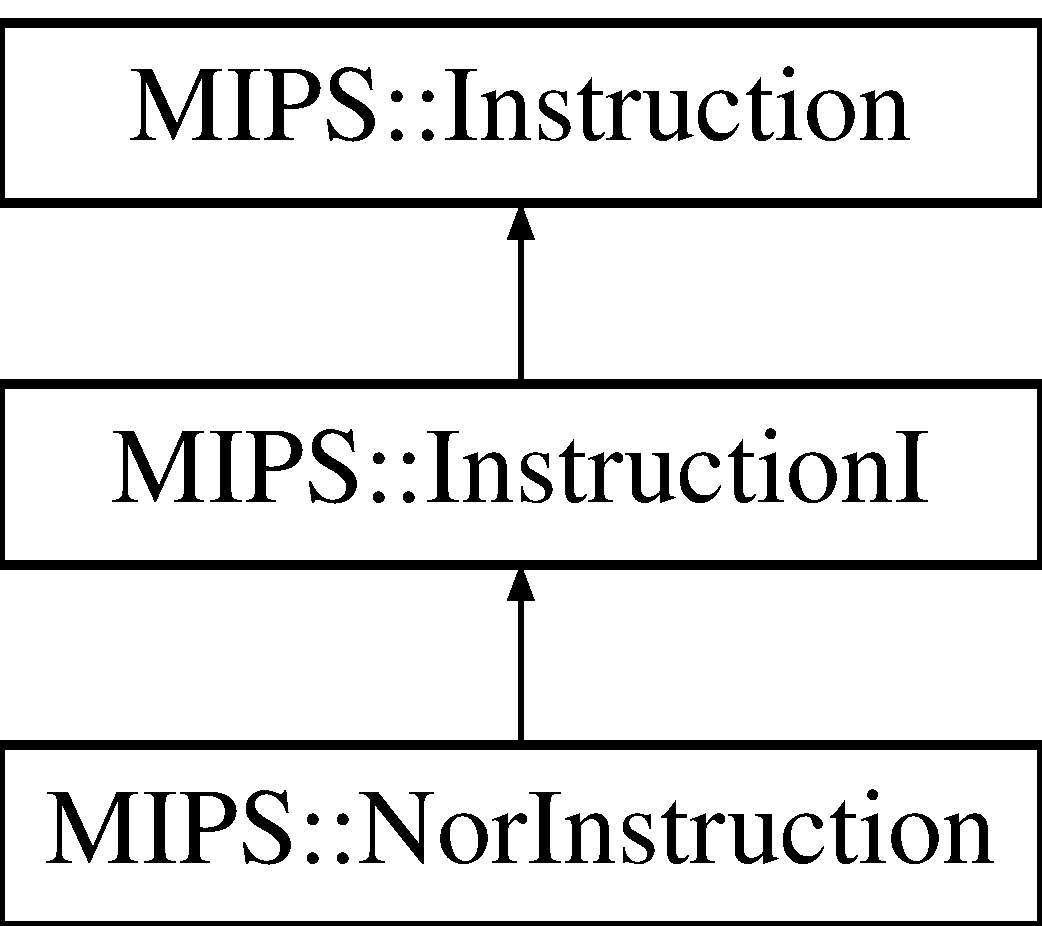
\includegraphics[height=3.000000cm]{classMIPS_1_1NorInstruction}
\end{center}
\end{figure}
\subsection*{Public Member Functions}
\begin{DoxyCompactItemize}
\item 
\hyperlink{classMIPS_1_1NorInstruction_a56d6fb7a2f54c446c06a8cba4b159d4f}{Nor\+Instruction} (\hyperlink{core_8hpp_a6074bae122ae7b527864eec42c728c3c}{bit8\+\_\+t} \hyperlink{classMIPS_1_1Instruction_a45cc6808b5dde8a5d41067d148b55476}{opcode}, \hyperlink{classMIPS_1_1Register}{Register} $\ast$\hyperlink{classMIPS_1_1InstructionI_a2be191d5b3dce505e2e626ec02eb4d62}{rs}, \hyperlink{classMIPS_1_1Register}{Register} $\ast$\hyperlink{classMIPS_1_1InstructionI_add1db07a5c954f35271de8c8a5737487}{rt}, \hyperlink{core_8hpp_a6074bae122ae7b527864eec42c728c3c}{bit8\+\_\+t} \hyperlink{classMIPS_1_1InstructionI_aa9b6da37c374c2ec8d96448d341e5e7d}{shamt}, \hyperlink{core_8hpp_a6074bae122ae7b527864eec42c728c3c}{bit8\+\_\+t} \hyperlink{classMIPS_1_1InstructionI_a5c6efcbbd233a7447c1fe24ea0a1e558}{funct})
\item 
\hyperlink{core_8hpp_adc265a970bc35995b5879784bbb3f1b7}{bit16\+\_\+t} \hyperlink{classMIPS_1_1NorInstruction_a68bb5cc9920bd63229f4c16c4edb5ab6}{execute} ()
\end{DoxyCompactItemize}
\subsection*{Additional Inherited Members}


\subsection{Detailed Description}
Classe que faz a operação de N\+OR no processador.

\begin{DoxyAuthor}{Author}
Felipe Dias 
\end{DoxyAuthor}


\subsection{Constructor \& Destructor Documentation}
\index{M\+I\+P\+S\+::\+Nor\+Instruction@{M\+I\+P\+S\+::\+Nor\+Instruction}!Nor\+Instruction@{Nor\+Instruction}}
\index{Nor\+Instruction@{Nor\+Instruction}!M\+I\+P\+S\+::\+Nor\+Instruction@{M\+I\+P\+S\+::\+Nor\+Instruction}}
\subsubsection[{\texorpdfstring{Nor\+Instruction(bit8\+\_\+t opcode, Register $\ast$rs, Register $\ast$rt, bit8\+\_\+t shamt, bit8\+\_\+t funct)}{NorInstruction(bit8_t opcode, Register *rs, Register *rt, bit8_t shamt, bit8_t funct)}}]{\setlength{\rightskip}{0pt plus 5cm}M\+I\+P\+S\+::\+Nor\+Instruction\+::\+Nor\+Instruction (
\begin{DoxyParamCaption}
\item[{{\bf bit8\+\_\+t}}]{opcode, }
\item[{{\bf Register} $\ast$}]{rs, }
\item[{{\bf Register} $\ast$}]{rt, }
\item[{{\bf bit8\+\_\+t}}]{shamt, }
\item[{{\bf bit8\+\_\+t}}]{funct}
\end{DoxyParamCaption}
)\hspace{0.3cm}{\ttfamily [inline]}}\hypertarget{classMIPS_1_1NorInstruction_a56d6fb7a2f54c446c06a8cba4b159d4f}{}\label{classMIPS_1_1NorInstruction_a56d6fb7a2f54c446c06a8cba4b159d4f}
Constroi uma nova instrução. 

\subsection{Member Function Documentation}
\index{M\+I\+P\+S\+::\+Nor\+Instruction@{M\+I\+P\+S\+::\+Nor\+Instruction}!execute@{execute}}
\index{execute@{execute}!M\+I\+P\+S\+::\+Nor\+Instruction@{M\+I\+P\+S\+::\+Nor\+Instruction}}
\subsubsection[{\texorpdfstring{execute()}{execute()}}]{\setlength{\rightskip}{0pt plus 5cm}{\bf bit16\+\_\+t} M\+I\+P\+S\+::\+Nor\+Instruction\+::execute (
\begin{DoxyParamCaption}
{}
\end{DoxyParamCaption}
)\hspace{0.3cm}{\ttfamily [virtual]}}\hypertarget{classMIPS_1_1NorInstruction_a68bb5cc9920bd63229f4c16c4edb5ab6}{}\label{classMIPS_1_1NorInstruction_a68bb5cc9920bd63229f4c16c4edb5ab6}
Função que executa a operação de soma.

\begin{DoxyReturn}{Returns}
resultado da operação 
\end{DoxyReturn}


Implements \hyperlink{classMIPS_1_1InstructionI_ae60fca5801bf5415cdff06d2aa11764f}{M\+I\+P\+S\+::\+InstructionI}.



The documentation for this class was generated from the following file\+:\begin{DoxyCompactItemize}
\item 
include/mips/instructions/format\+\_\+\+I/\hyperlink{nor_8hpp}{nor.\+hpp}\end{DoxyCompactItemize}

\hypertarget{classMIPS_1_1OnesInstruction}{}\section{M\+I\+PS\+:\+:Ones\+Instruction Class Reference}
\label{classMIPS_1_1OnesInstruction}\index{M\+I\+P\+S\+::\+Ones\+Instruction@{M\+I\+P\+S\+::\+Ones\+Instruction}}


{\ttfamily \#include $<$ones.\+hpp$>$}

Inheritance diagram for M\+I\+PS\+:\+:Ones\+Instruction\+:\begin{figure}[H]
\begin{center}
\leavevmode
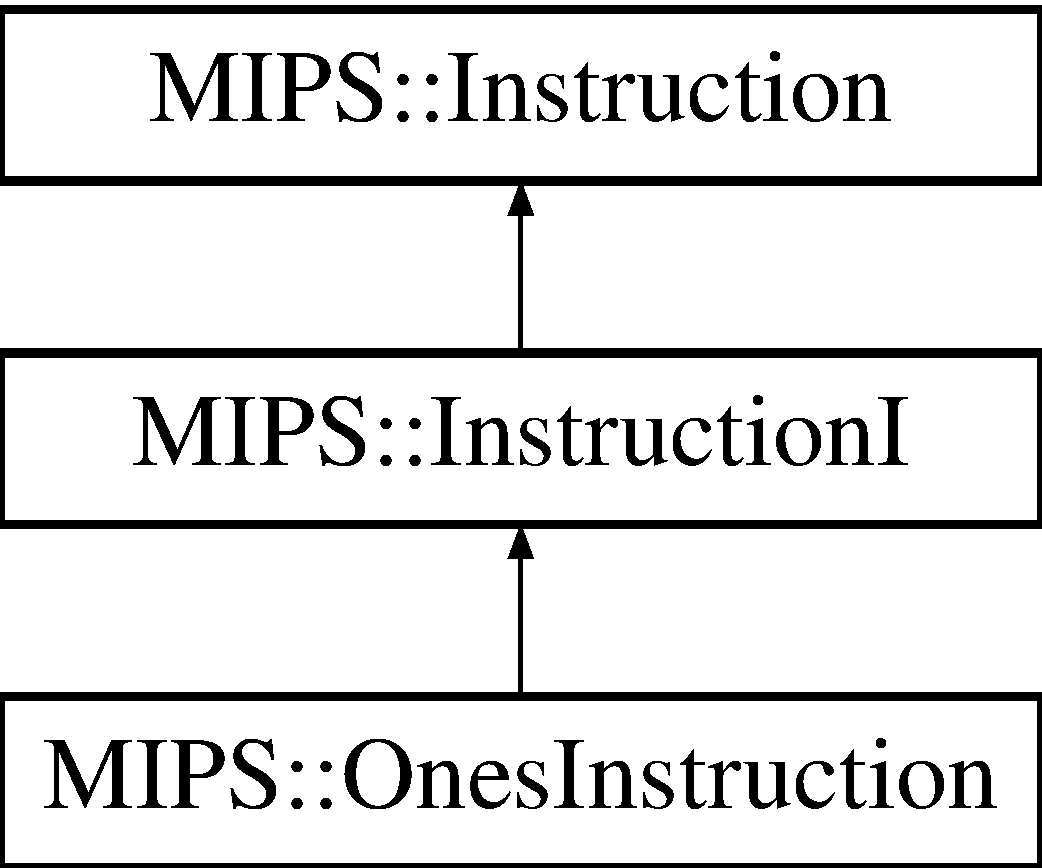
\includegraphics[height=3.000000cm]{classMIPS_1_1OnesInstruction}
\end{center}
\end{figure}
\subsection*{Public Member Functions}
\begin{DoxyCompactItemize}
\item 
\hyperlink{classMIPS_1_1OnesInstruction_ac12775ee6e4e5c1a33636384c4f6244e}{Ones\+Instruction} (\hyperlink{core_8hpp_a6074bae122ae7b527864eec42c728c3c}{bit8\+\_\+t} \hyperlink{classMIPS_1_1Instruction_a45cc6808b5dde8a5d41067d148b55476}{opcode}, \hyperlink{classMIPS_1_1Register}{Register} $\ast$\hyperlink{classMIPS_1_1InstructionI_a2be191d5b3dce505e2e626ec02eb4d62}{rs}, \hyperlink{classMIPS_1_1Register}{Register} $\ast$\hyperlink{classMIPS_1_1InstructionI_add1db07a5c954f35271de8c8a5737487}{rt}, \hyperlink{core_8hpp_a6074bae122ae7b527864eec42c728c3c}{bit8\+\_\+t} \hyperlink{classMIPS_1_1InstructionI_aa9b6da37c374c2ec8d96448d341e5e7d}{shamt}, \hyperlink{core_8hpp_a6074bae122ae7b527864eec42c728c3c}{bit8\+\_\+t} \hyperlink{classMIPS_1_1InstructionI_a5c6efcbbd233a7447c1fe24ea0a1e558}{funct})
\item 
\hyperlink{core_8hpp_adc265a970bc35995b5879784bbb3f1b7}{bit16\+\_\+t} \hyperlink{classMIPS_1_1OnesInstruction_aeab25fd32df5c092d4f426371f3f1ff3}{execute} ()
\end{DoxyCompactItemize}
\subsection*{Additional Inherited Members}


\subsection{Detailed Description}
Classe que faz a operação de O\+N\+ES no processador.

\begin{DoxyAuthor}{Author}
Felipe Dias 
\end{DoxyAuthor}


\subsection{Constructor \& Destructor Documentation}
\index{M\+I\+P\+S\+::\+Ones\+Instruction@{M\+I\+P\+S\+::\+Ones\+Instruction}!Ones\+Instruction@{Ones\+Instruction}}
\index{Ones\+Instruction@{Ones\+Instruction}!M\+I\+P\+S\+::\+Ones\+Instruction@{M\+I\+P\+S\+::\+Ones\+Instruction}}
\subsubsection[{\texorpdfstring{Ones\+Instruction(bit8\+\_\+t opcode, Register $\ast$rs, Register $\ast$rt, bit8\+\_\+t shamt, bit8\+\_\+t funct)}{OnesInstruction(bit8_t opcode, Register *rs, Register *rt, bit8_t shamt, bit8_t funct)}}]{\setlength{\rightskip}{0pt plus 5cm}M\+I\+P\+S\+::\+Ones\+Instruction\+::\+Ones\+Instruction (
\begin{DoxyParamCaption}
\item[{{\bf bit8\+\_\+t}}]{opcode, }
\item[{{\bf Register} $\ast$}]{rs, }
\item[{{\bf Register} $\ast$}]{rt, }
\item[{{\bf bit8\+\_\+t}}]{shamt, }
\item[{{\bf bit8\+\_\+t}}]{funct}
\end{DoxyParamCaption}
)\hspace{0.3cm}{\ttfamily [inline]}}\hypertarget{classMIPS_1_1OnesInstruction_ac12775ee6e4e5c1a33636384c4f6244e}{}\label{classMIPS_1_1OnesInstruction_ac12775ee6e4e5c1a33636384c4f6244e}
Constroi uma nova instrução. 

\subsection{Member Function Documentation}
\index{M\+I\+P\+S\+::\+Ones\+Instruction@{M\+I\+P\+S\+::\+Ones\+Instruction}!execute@{execute}}
\index{execute@{execute}!M\+I\+P\+S\+::\+Ones\+Instruction@{M\+I\+P\+S\+::\+Ones\+Instruction}}
\subsubsection[{\texorpdfstring{execute()}{execute()}}]{\setlength{\rightskip}{0pt plus 5cm}{\bf bit16\+\_\+t} M\+I\+P\+S\+::\+Ones\+Instruction\+::execute (
\begin{DoxyParamCaption}
{}
\end{DoxyParamCaption}
)\hspace{0.3cm}{\ttfamily [virtual]}}\hypertarget{classMIPS_1_1OnesInstruction_aeab25fd32df5c092d4f426371f3f1ff3}{}\label{classMIPS_1_1OnesInstruction_aeab25fd32df5c092d4f426371f3f1ff3}
Função que executa a operação de soma.

\begin{DoxyReturn}{Returns}
resultado da operação 
\end{DoxyReturn}


Implements \hyperlink{classMIPS_1_1InstructionI_ae60fca5801bf5415cdff06d2aa11764f}{M\+I\+P\+S\+::\+InstructionI}.



The documentation for this class was generated from the following file\+:\begin{DoxyCompactItemize}
\item 
include/mips/instructions/format\+\_\+\+I/\hyperlink{ones_8hpp}{ones.\+hpp}\end{DoxyCompactItemize}

\hypertarget{classMIPS_1_1OrInstruction}{}\section{M\+I\+PS\+:\+:Or\+Instruction Class Reference}
\label{classMIPS_1_1OrInstruction}\index{M\+I\+P\+S\+::\+Or\+Instruction@{M\+I\+P\+S\+::\+Or\+Instruction}}


{\ttfamily \#include $<$or.\+hpp$>$}

Inheritance diagram for M\+I\+PS\+:\+:Or\+Instruction\+:\begin{figure}[H]
\begin{center}
\leavevmode
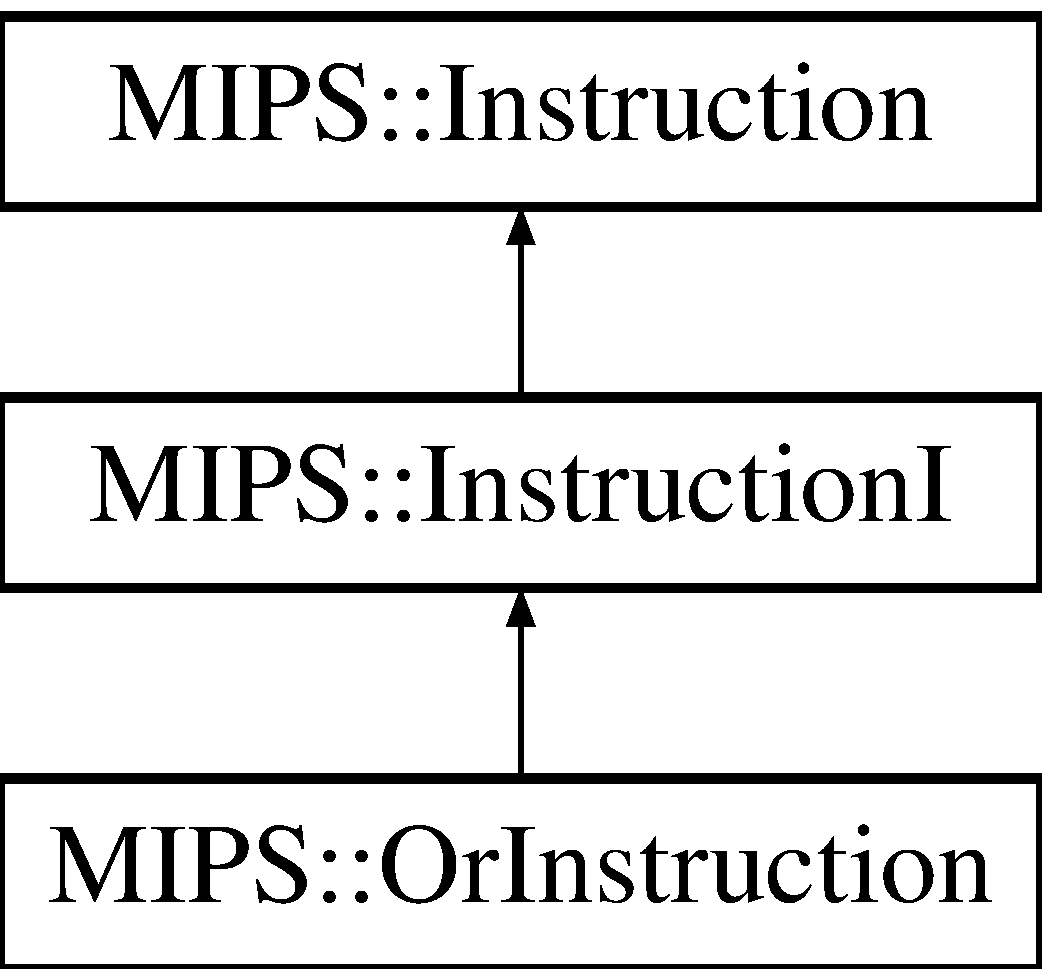
\includegraphics[height=3.000000cm]{classMIPS_1_1OrInstruction}
\end{center}
\end{figure}
\subsection*{Public Member Functions}
\begin{DoxyCompactItemize}
\item 
\hyperlink{classMIPS_1_1OrInstruction_a5e9d9d3677eaf08e528c186149d59662}{Or\+Instruction} (\hyperlink{core_8hpp_a6074bae122ae7b527864eec42c728c3c}{bit8\+\_\+t} \hyperlink{classMIPS_1_1Instruction_a45cc6808b5dde8a5d41067d148b55476}{opcode}, \hyperlink{classMIPS_1_1Register}{Register} $\ast$\hyperlink{classMIPS_1_1InstructionI_a2be191d5b3dce505e2e626ec02eb4d62}{rs}, \hyperlink{classMIPS_1_1Register}{Register} $\ast$\hyperlink{classMIPS_1_1InstructionI_add1db07a5c954f35271de8c8a5737487}{rt}, \hyperlink{core_8hpp_a6074bae122ae7b527864eec42c728c3c}{bit8\+\_\+t} \hyperlink{classMIPS_1_1InstructionI_aa9b6da37c374c2ec8d96448d341e5e7d}{shamt}, \hyperlink{core_8hpp_a6074bae122ae7b527864eec42c728c3c}{bit8\+\_\+t} \hyperlink{classMIPS_1_1InstructionI_a5c6efcbbd233a7447c1fe24ea0a1e558}{funct})
\item 
\hyperlink{core_8hpp_adc265a970bc35995b5879784bbb3f1b7}{bit16\+\_\+t} \hyperlink{classMIPS_1_1OrInstruction_a89859e0bcb3e5ed7f1c53f33f627f041}{execute} ()
\end{DoxyCompactItemize}
\subsection*{Additional Inherited Members}


\subsection{Detailed Description}
Classe que faz a operação de OR no processador.

\begin{DoxyAuthor}{Author}
Lucas Fonseca dos Santos 
\end{DoxyAuthor}


\subsection{Constructor \& Destructor Documentation}
\index{M\+I\+P\+S\+::\+Or\+Instruction@{M\+I\+P\+S\+::\+Or\+Instruction}!Or\+Instruction@{Or\+Instruction}}
\index{Or\+Instruction@{Or\+Instruction}!M\+I\+P\+S\+::\+Or\+Instruction@{M\+I\+P\+S\+::\+Or\+Instruction}}
\subsubsection[{\texorpdfstring{Or\+Instruction(bit8\+\_\+t opcode, Register $\ast$rs, Register $\ast$rt, bit8\+\_\+t shamt, bit8\+\_\+t funct)}{OrInstruction(bit8_t opcode, Register *rs, Register *rt, bit8_t shamt, bit8_t funct)}}]{\setlength{\rightskip}{0pt plus 5cm}M\+I\+P\+S\+::\+Or\+Instruction\+::\+Or\+Instruction (
\begin{DoxyParamCaption}
\item[{{\bf bit8\+\_\+t}}]{opcode, }
\item[{{\bf Register} $\ast$}]{rs, }
\item[{{\bf Register} $\ast$}]{rt, }
\item[{{\bf bit8\+\_\+t}}]{shamt, }
\item[{{\bf bit8\+\_\+t}}]{funct}
\end{DoxyParamCaption}
)\hspace{0.3cm}{\ttfamily [inline]}}\hypertarget{classMIPS_1_1OrInstruction_a5e9d9d3677eaf08e528c186149d59662}{}\label{classMIPS_1_1OrInstruction_a5e9d9d3677eaf08e528c186149d59662}
Constroi uma nova instrução. 

\subsection{Member Function Documentation}
\index{M\+I\+P\+S\+::\+Or\+Instruction@{M\+I\+P\+S\+::\+Or\+Instruction}!execute@{execute}}
\index{execute@{execute}!M\+I\+P\+S\+::\+Or\+Instruction@{M\+I\+P\+S\+::\+Or\+Instruction}}
\subsubsection[{\texorpdfstring{execute()}{execute()}}]{\setlength{\rightskip}{0pt plus 5cm}{\bf bit16\+\_\+t} M\+I\+P\+S\+::\+Or\+Instruction\+::execute (
\begin{DoxyParamCaption}
{}
\end{DoxyParamCaption}
)\hspace{0.3cm}{\ttfamily [virtual]}}\hypertarget{classMIPS_1_1OrInstruction_a89859e0bcb3e5ed7f1c53f33f627f041}{}\label{classMIPS_1_1OrInstruction_a89859e0bcb3e5ed7f1c53f33f627f041}
Função que executa a operação de \hyperlink{classMIPS_1_1OrInstruction}{Or\+Instruction}. 

Implements \hyperlink{classMIPS_1_1InstructionI_ae60fca5801bf5415cdff06d2aa11764f}{M\+I\+P\+S\+::\+InstructionI}.



The documentation for this class was generated from the following file\+:\begin{DoxyCompactItemize}
\item 
include/mips/instructions/format\+\_\+\+I/\hyperlink{or_8hpp}{or.\+hpp}\end{DoxyCompactItemize}

\hypertarget{classMIPS_1_1OrnotbInstruction}{}\section{M\+I\+PS\+:\+:Ornotb\+Instruction Class Reference}
\label{classMIPS_1_1OrnotbInstruction}\index{M\+I\+P\+S\+::\+Ornotb\+Instruction@{M\+I\+P\+S\+::\+Ornotb\+Instruction}}


{\ttfamily \#include $<$ornotb.\+hpp$>$}

Inheritance diagram for M\+I\+PS\+:\+:Ornotb\+Instruction\+:\begin{figure}[H]
\begin{center}
\leavevmode
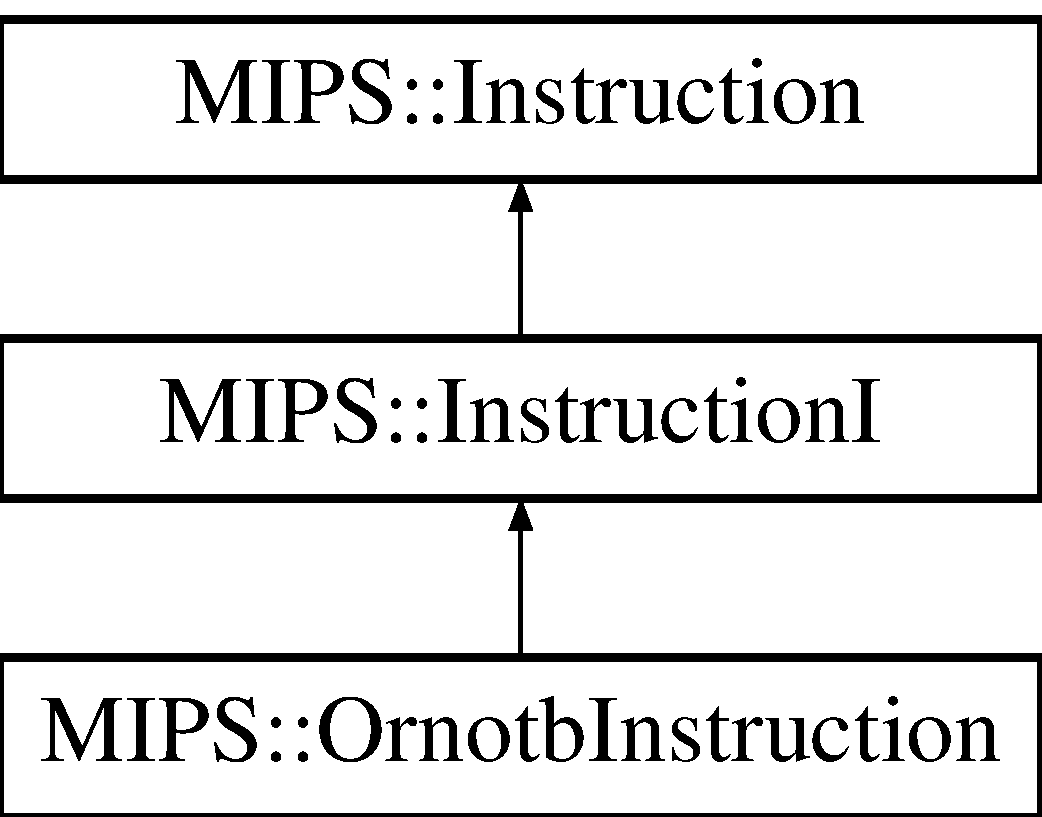
\includegraphics[height=3.000000cm]{classMIPS_1_1OrnotbInstruction}
\end{center}
\end{figure}
\subsection*{Public Member Functions}
\begin{DoxyCompactItemize}
\item 
\hyperlink{classMIPS_1_1OrnotbInstruction_aea52181c168c690a024590196516c89e}{Ornotb\+Instruction} (\hyperlink{core_8hpp_a6074bae122ae7b527864eec42c728c3c}{bit8\+\_\+t} \hyperlink{classMIPS_1_1Instruction_a45cc6808b5dde8a5d41067d148b55476}{opcode}, \hyperlink{classMIPS_1_1Register}{Register} $\ast$\hyperlink{classMIPS_1_1InstructionI_a2be191d5b3dce505e2e626ec02eb4d62}{rs}, \hyperlink{classMIPS_1_1Register}{Register} $\ast$\hyperlink{classMIPS_1_1InstructionI_add1db07a5c954f35271de8c8a5737487}{rt}, \hyperlink{core_8hpp_a6074bae122ae7b527864eec42c728c3c}{bit8\+\_\+t} \hyperlink{classMIPS_1_1InstructionI_aa9b6da37c374c2ec8d96448d341e5e7d}{shamt}, \hyperlink{core_8hpp_a6074bae122ae7b527864eec42c728c3c}{bit8\+\_\+t} \hyperlink{classMIPS_1_1InstructionI_a5c6efcbbd233a7447c1fe24ea0a1e558}{funct})
\item 
\hyperlink{core_8hpp_adc265a970bc35995b5879784bbb3f1b7}{bit16\+\_\+t} \hyperlink{classMIPS_1_1OrnotbInstruction_a47aac4ac3ef0ee8c6a694189f26bd80e}{execute} ()
\end{DoxyCompactItemize}
\subsection*{Additional Inherited Members}


\subsection{Detailed Description}
Classe que faz a operação de ornotb no processador.

\begin{DoxyAuthor}{Author}
Lucas Pereira 
\end{DoxyAuthor}


\subsection{Constructor \& Destructor Documentation}
\index{M\+I\+P\+S\+::\+Ornotb\+Instruction@{M\+I\+P\+S\+::\+Ornotb\+Instruction}!Ornotb\+Instruction@{Ornotb\+Instruction}}
\index{Ornotb\+Instruction@{Ornotb\+Instruction}!M\+I\+P\+S\+::\+Ornotb\+Instruction@{M\+I\+P\+S\+::\+Ornotb\+Instruction}}
\subsubsection[{\texorpdfstring{Ornotb\+Instruction(bit8\+\_\+t opcode, Register $\ast$rs, Register $\ast$rt, bit8\+\_\+t shamt, bit8\+\_\+t funct)}{OrnotbInstruction(bit8_t opcode, Register *rs, Register *rt, bit8_t shamt, bit8_t funct)}}]{\setlength{\rightskip}{0pt plus 5cm}M\+I\+P\+S\+::\+Ornotb\+Instruction\+::\+Ornotb\+Instruction (
\begin{DoxyParamCaption}
\item[{{\bf bit8\+\_\+t}}]{opcode, }
\item[{{\bf Register} $\ast$}]{rs, }
\item[{{\bf Register} $\ast$}]{rt, }
\item[{{\bf bit8\+\_\+t}}]{shamt, }
\item[{{\bf bit8\+\_\+t}}]{funct}
\end{DoxyParamCaption}
)\hspace{0.3cm}{\ttfamily [inline]}}\hypertarget{classMIPS_1_1OrnotbInstruction_aea52181c168c690a024590196516c89e}{}\label{classMIPS_1_1OrnotbInstruction_aea52181c168c690a024590196516c89e}
Constroi uma nova instrução. 

\subsection{Member Function Documentation}
\index{M\+I\+P\+S\+::\+Ornotb\+Instruction@{M\+I\+P\+S\+::\+Ornotb\+Instruction}!execute@{execute}}
\index{execute@{execute}!M\+I\+P\+S\+::\+Ornotb\+Instruction@{M\+I\+P\+S\+::\+Ornotb\+Instruction}}
\subsubsection[{\texorpdfstring{execute()}{execute()}}]{\setlength{\rightskip}{0pt plus 5cm}{\bf bit16\+\_\+t} M\+I\+P\+S\+::\+Ornotb\+Instruction\+::execute (
\begin{DoxyParamCaption}
{}
\end{DoxyParamCaption}
)\hspace{0.3cm}{\ttfamily [virtual]}}\hypertarget{classMIPS_1_1OrnotbInstruction_a47aac4ac3ef0ee8c6a694189f26bd80e}{}\label{classMIPS_1_1OrnotbInstruction_a47aac4ac3ef0ee8c6a694189f26bd80e}
Função que executa a operação de \hyperlink{classMIPS_1_1OrnotbInstruction}{Ornotb\+Instruction}. 

Implements \hyperlink{classMIPS_1_1InstructionI_ae60fca5801bf5415cdff06d2aa11764f}{M\+I\+P\+S\+::\+InstructionI}.



The documentation for this class was generated from the following file\+:\begin{DoxyCompactItemize}
\item 
include/mips/instructions/format\+\_\+\+I/\hyperlink{ornotb_8hpp}{ornotb.\+hpp}\end{DoxyCompactItemize}

\hypertarget{classMIPS_1_1PassaInstruction}{}\section{M\+I\+PS\+:\+:Passa\+Instruction Class Reference}
\label{classMIPS_1_1PassaInstruction}\index{M\+I\+P\+S\+::\+Passa\+Instruction@{M\+I\+P\+S\+::\+Passa\+Instruction}}


{\ttfamily \#include $<$passa.\+hpp$>$}

Inheritance diagram for M\+I\+PS\+:\+:Passa\+Instruction\+:\begin{figure}[H]
\begin{center}
\leavevmode
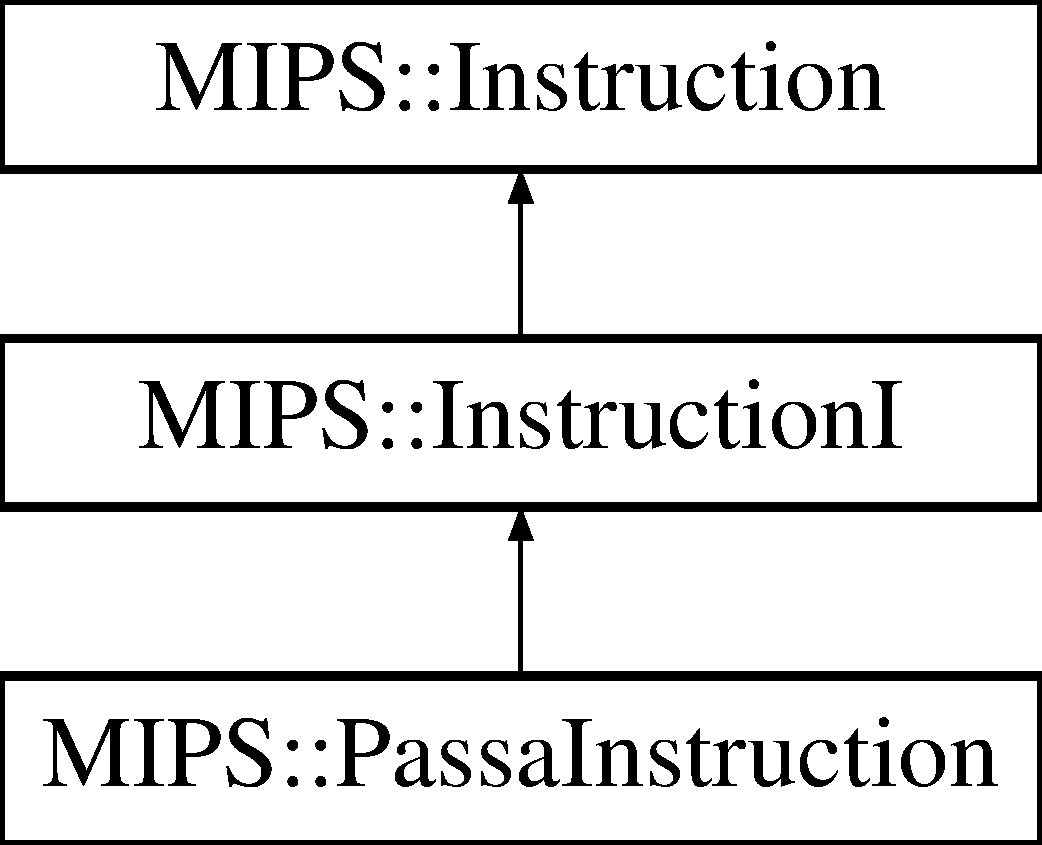
\includegraphics[height=3.000000cm]{classMIPS_1_1PassaInstruction}
\end{center}
\end{figure}
\subsection*{Public Member Functions}
\begin{DoxyCompactItemize}
\item 
\hyperlink{classMIPS_1_1PassaInstruction_acc56ffbb33152fef680a714c2ba4a154}{Passa\+Instruction} (\hyperlink{core_8hpp_a6074bae122ae7b527864eec42c728c3c}{bit8\+\_\+t} \hyperlink{classMIPS_1_1Instruction_a45cc6808b5dde8a5d41067d148b55476}{opcode}, \hyperlink{classMIPS_1_1Register}{Register} $\ast$\hyperlink{classMIPS_1_1InstructionI_a2be191d5b3dce505e2e626ec02eb4d62}{rs}, \hyperlink{classMIPS_1_1Register}{Register} $\ast$\hyperlink{classMIPS_1_1InstructionI_add1db07a5c954f35271de8c8a5737487}{rt}, \hyperlink{core_8hpp_a6074bae122ae7b527864eec42c728c3c}{bit8\+\_\+t} \hyperlink{classMIPS_1_1InstructionI_aa9b6da37c374c2ec8d96448d341e5e7d}{shamt}, \hyperlink{core_8hpp_a6074bae122ae7b527864eec42c728c3c}{bit8\+\_\+t} \hyperlink{classMIPS_1_1InstructionI_a5c6efcbbd233a7447c1fe24ea0a1e558}{funct})
\item 
\hyperlink{core_8hpp_adc265a970bc35995b5879784bbb3f1b7}{bit16\+\_\+t} \hyperlink{classMIPS_1_1PassaInstruction_ae23b43bfb84d2ef69fa25e50fb5b6072}{execute} ()
\end{DoxyCompactItemize}
\subsection*{Additional Inherited Members}


\subsection{Detailed Description}
Classe que faz a operação de P\+A\+S\+SA no processador.

\begin{DoxyAuthor}{Author}
Matheus Nogueira 
\end{DoxyAuthor}


\subsection{Constructor \& Destructor Documentation}
\index{M\+I\+P\+S\+::\+Passa\+Instruction@{M\+I\+P\+S\+::\+Passa\+Instruction}!Passa\+Instruction@{Passa\+Instruction}}
\index{Passa\+Instruction@{Passa\+Instruction}!M\+I\+P\+S\+::\+Passa\+Instruction@{M\+I\+P\+S\+::\+Passa\+Instruction}}
\subsubsection[{\texorpdfstring{Passa\+Instruction(bit8\+\_\+t opcode, Register $\ast$rs, Register $\ast$rt, bit8\+\_\+t shamt, bit8\+\_\+t funct)}{PassaInstruction(bit8_t opcode, Register *rs, Register *rt, bit8_t shamt, bit8_t funct)}}]{\setlength{\rightskip}{0pt plus 5cm}M\+I\+P\+S\+::\+Passa\+Instruction\+::\+Passa\+Instruction (
\begin{DoxyParamCaption}
\item[{{\bf bit8\+\_\+t}}]{opcode, }
\item[{{\bf Register} $\ast$}]{rs, }
\item[{{\bf Register} $\ast$}]{rt, }
\item[{{\bf bit8\+\_\+t}}]{shamt, }
\item[{{\bf bit8\+\_\+t}}]{funct}
\end{DoxyParamCaption}
)\hspace{0.3cm}{\ttfamily [inline]}}\hypertarget{classMIPS_1_1PassaInstruction_acc56ffbb33152fef680a714c2ba4a154}{}\label{classMIPS_1_1PassaInstruction_acc56ffbb33152fef680a714c2ba4a154}
Constroi uma nova instrução. 

\subsection{Member Function Documentation}
\index{M\+I\+P\+S\+::\+Passa\+Instruction@{M\+I\+P\+S\+::\+Passa\+Instruction}!execute@{execute}}
\index{execute@{execute}!M\+I\+P\+S\+::\+Passa\+Instruction@{M\+I\+P\+S\+::\+Passa\+Instruction}}
\subsubsection[{\texorpdfstring{execute()}{execute()}}]{\setlength{\rightskip}{0pt plus 5cm}{\bf bit16\+\_\+t} M\+I\+P\+S\+::\+Passa\+Instruction\+::execute (
\begin{DoxyParamCaption}
{}
\end{DoxyParamCaption}
)\hspace{0.3cm}{\ttfamily [virtual]}}\hypertarget{classMIPS_1_1PassaInstruction_ae23b43bfb84d2ef69fa25e50fb5b6072}{}\label{classMIPS_1_1PassaInstruction_ae23b43bfb84d2ef69fa25e50fb5b6072}
Função que executa a operação de soma.

\begin{DoxyReturn}{Returns}
resultado da operação 
\end{DoxyReturn}


Implements \hyperlink{classMIPS_1_1InstructionI_ae60fca5801bf5415cdff06d2aa11764f}{M\+I\+P\+S\+::\+InstructionI}.



The documentation for this class was generated from the following file\+:\begin{DoxyCompactItemize}
\item 
include/mips/instructions/format\+\_\+\+I/\hyperlink{passa_8hpp}{passa.\+hpp}\end{DoxyCompactItemize}

\hypertarget{classMIPS_1_1PassNotAInstruction}{}\section{M\+I\+PS\+:\+:Pass\+Not\+A\+Instruction Class Reference}
\label{classMIPS_1_1PassNotAInstruction}\index{M\+I\+P\+S\+::\+Pass\+Not\+A\+Instruction@{M\+I\+P\+S\+::\+Pass\+Not\+A\+Instruction}}


{\ttfamily \#include $<$passnota.\+hpp$>$}

Inheritance diagram for M\+I\+PS\+:\+:Pass\+Not\+A\+Instruction\+:\begin{figure}[H]
\begin{center}
\leavevmode
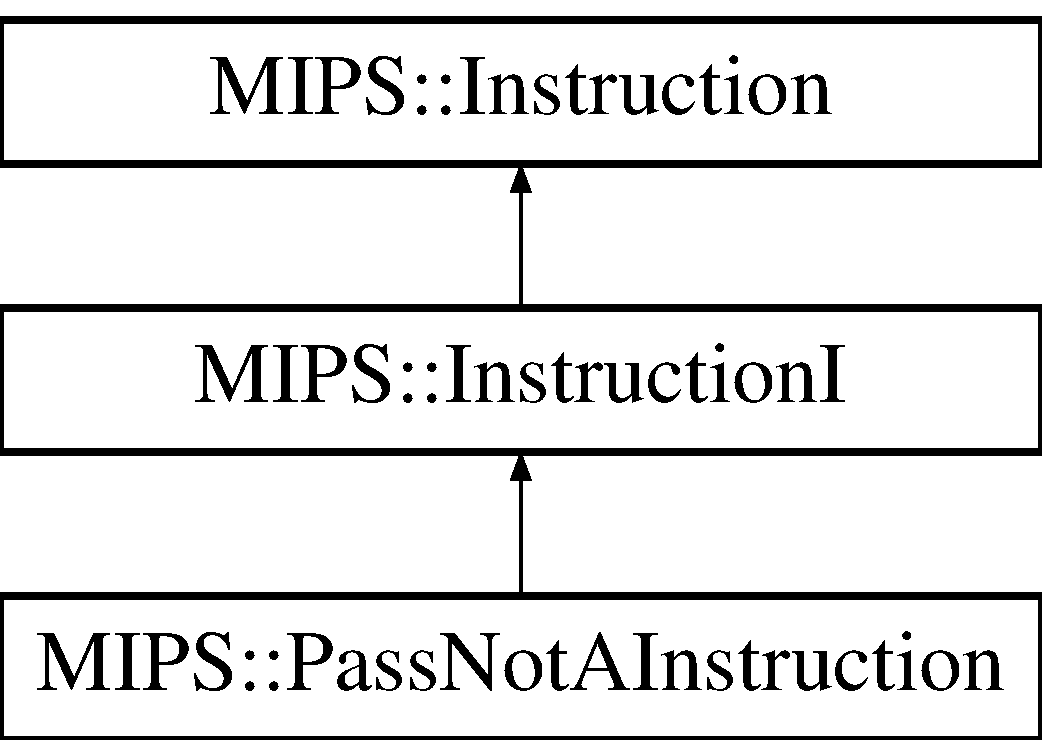
\includegraphics[height=3.000000cm]{classMIPS_1_1PassNotAInstruction}
\end{center}
\end{figure}
\subsection*{Public Member Functions}
\begin{DoxyCompactItemize}
\item 
\hyperlink{classMIPS_1_1PassNotAInstruction_a4e68ad0b8200cd75f2b08346e7b2031a}{Pass\+Not\+A\+Instruction} (\hyperlink{core_8hpp_a6074bae122ae7b527864eec42c728c3c}{bit8\+\_\+t} \hyperlink{classMIPS_1_1Instruction_a45cc6808b5dde8a5d41067d148b55476}{opcode}, \hyperlink{classMIPS_1_1Register}{Register} $\ast$\hyperlink{classMIPS_1_1InstructionI_a2be191d5b3dce505e2e626ec02eb4d62}{rs}, \hyperlink{classMIPS_1_1Register}{Register} $\ast$\hyperlink{classMIPS_1_1InstructionI_add1db07a5c954f35271de8c8a5737487}{rt}, \hyperlink{core_8hpp_a6074bae122ae7b527864eec42c728c3c}{bit8\+\_\+t} \hyperlink{classMIPS_1_1InstructionI_aa9b6da37c374c2ec8d96448d341e5e7d}{shamt}, \hyperlink{core_8hpp_a6074bae122ae7b527864eec42c728c3c}{bit8\+\_\+t} \hyperlink{classMIPS_1_1InstructionI_a5c6efcbbd233a7447c1fe24ea0a1e558}{funct})
\item 
\hyperlink{core_8hpp_adc265a970bc35995b5879784bbb3f1b7}{bit16\+\_\+t} \hyperlink{classMIPS_1_1PassNotAInstruction_a30b9bdb1feac1adb44e70a3a0eb85cb4}{execute} ()
\end{DoxyCompactItemize}
\subsection*{Additional Inherited Members}


\subsection{Detailed Description}
Classe que faz a operação de P\+A\+S\+S\+N\+O\+TA no processador.

\begin{DoxyAuthor}{Author}
Felipe Dias 
\end{DoxyAuthor}


\subsection{Constructor \& Destructor Documentation}
\index{M\+I\+P\+S\+::\+Pass\+Not\+A\+Instruction@{M\+I\+P\+S\+::\+Pass\+Not\+A\+Instruction}!Pass\+Not\+A\+Instruction@{Pass\+Not\+A\+Instruction}}
\index{Pass\+Not\+A\+Instruction@{Pass\+Not\+A\+Instruction}!M\+I\+P\+S\+::\+Pass\+Not\+A\+Instruction@{M\+I\+P\+S\+::\+Pass\+Not\+A\+Instruction}}
\subsubsection[{\texorpdfstring{Pass\+Not\+A\+Instruction(bit8\+\_\+t opcode, Register $\ast$rs, Register $\ast$rt, bit8\+\_\+t shamt, bit8\+\_\+t funct)}{PassNotAInstruction(bit8_t opcode, Register *rs, Register *rt, bit8_t shamt, bit8_t funct)}}]{\setlength{\rightskip}{0pt plus 5cm}M\+I\+P\+S\+::\+Pass\+Not\+A\+Instruction\+::\+Pass\+Not\+A\+Instruction (
\begin{DoxyParamCaption}
\item[{{\bf bit8\+\_\+t}}]{opcode, }
\item[{{\bf Register} $\ast$}]{rs, }
\item[{{\bf Register} $\ast$}]{rt, }
\item[{{\bf bit8\+\_\+t}}]{shamt, }
\item[{{\bf bit8\+\_\+t}}]{funct}
\end{DoxyParamCaption}
)\hspace{0.3cm}{\ttfamily [inline]}}\hypertarget{classMIPS_1_1PassNotAInstruction_a4e68ad0b8200cd75f2b08346e7b2031a}{}\label{classMIPS_1_1PassNotAInstruction_a4e68ad0b8200cd75f2b08346e7b2031a}
Constroi uma nova instrução. 

\subsection{Member Function Documentation}
\index{M\+I\+P\+S\+::\+Pass\+Not\+A\+Instruction@{M\+I\+P\+S\+::\+Pass\+Not\+A\+Instruction}!execute@{execute}}
\index{execute@{execute}!M\+I\+P\+S\+::\+Pass\+Not\+A\+Instruction@{M\+I\+P\+S\+::\+Pass\+Not\+A\+Instruction}}
\subsubsection[{\texorpdfstring{execute()}{execute()}}]{\setlength{\rightskip}{0pt plus 5cm}{\bf bit16\+\_\+t} M\+I\+P\+S\+::\+Pass\+Not\+A\+Instruction\+::execute (
\begin{DoxyParamCaption}
{}
\end{DoxyParamCaption}
)\hspace{0.3cm}{\ttfamily [virtual]}}\hypertarget{classMIPS_1_1PassNotAInstruction_a30b9bdb1feac1adb44e70a3a0eb85cb4}{}\label{classMIPS_1_1PassNotAInstruction_a30b9bdb1feac1adb44e70a3a0eb85cb4}
Função que executa a operação de soma.

\begin{DoxyReturn}{Returns}
resultado da operação 
\end{DoxyReturn}


Implements \hyperlink{classMIPS_1_1InstructionI_ae60fca5801bf5415cdff06d2aa11764f}{M\+I\+P\+S\+::\+InstructionI}.



The documentation for this class was generated from the following file\+:\begin{DoxyCompactItemize}
\item 
include/mips/instructions/format\+\_\+\+I/\hyperlink{passnota_8hpp}{passnota.\+hpp}\end{DoxyCompactItemize}

\hypertarget{classMIPS_1_1Queue}{}\section{M\+I\+PS\+:\+:Queue$<$ T $>$ Class Template Reference}
\label{classMIPS_1_1Queue}\index{M\+I\+P\+S\+::\+Queue$<$ T $>$@{M\+I\+P\+S\+::\+Queue$<$ T $>$}}


{\ttfamily \#include $<$queue.\+hpp$>$}

\subsection*{Classes}
\begin{DoxyCompactItemize}
\item 
struct \hyperlink{structMIPS_1_1Queue_1_1Node}{Node}
\end{DoxyCompactItemize}
\subsection*{Public Member Functions}
\begin{DoxyCompactItemize}
\item 
\hyperlink{classMIPS_1_1Queue_a9e0601a711a1cca386a294b307016d87}{Queue} ()
\item 
\hyperlink{classMIPS_1_1Queue_aec877c1c927ec1fae8b7a1db1b8a3eb5}{$\sim$\+Queue} ()
\item 
void \hyperlink{classMIPS_1_1Queue_a77b7b0d1c09253d3efc665f75f3dee45}{push} (T \&elem)
\item 
T \hyperlink{classMIPS_1_1Queue_a6a1fb36a33fe4ded5eb8e6c4dd754c54}{pop} ()
\item 
T \hyperlink{classMIPS_1_1Queue_adeb864dfe03bceff01a57270337987ad}{get} (size\+\_\+t pos)
\item 
size\+\_\+t \hyperlink{classMIPS_1_1Queue_a894681d26fc3e3bf2665a1b81cc18341}{size} ()
\end{DoxyCompactItemize}


\subsection{Detailed Description}
\subsubsection*{template$<$typename T$>$\\*
class M\+I\+P\+S\+::\+Queue$<$ T $>$}

Fila genérica que utiliza template para auxiliar em seu reuso.


\begin{DoxyParams}{Parameters}
{\em Matheus} & Nogueira \\
\hline
\end{DoxyParams}


\subsection{Constructor \& Destructor Documentation}
\index{M\+I\+P\+S\+::\+Queue@{M\+I\+P\+S\+::\+Queue}!Queue@{Queue}}
\index{Queue@{Queue}!M\+I\+P\+S\+::\+Queue@{M\+I\+P\+S\+::\+Queue}}
\subsubsection[{\texorpdfstring{Queue()}{Queue()}}]{\setlength{\rightskip}{0pt plus 5cm}template$<$typename T$>$ {\bf M\+I\+P\+S\+::\+Queue}$<$ T $>$\+::{\bf Queue} (
\begin{DoxyParamCaption}
{}
\end{DoxyParamCaption}
)\hspace{0.3cm}{\ttfamily [inline]}}\hypertarget{classMIPS_1_1Queue_a9e0601a711a1cca386a294b307016d87}{}\label{classMIPS_1_1Queue_a9e0601a711a1cca386a294b307016d87}
Cria uma nova fila encadeada. $<$ Cabeça da fila

$<$ Número de elementos da fila \index{M\+I\+P\+S\+::\+Queue@{M\+I\+P\+S\+::\+Queue}!````~Queue@{$\sim$\+Queue}}
\index{````~Queue@{$\sim$\+Queue}!M\+I\+P\+S\+::\+Queue@{M\+I\+P\+S\+::\+Queue}}
\subsubsection[{\texorpdfstring{$\sim$\+Queue()}{~Queue()}}]{\setlength{\rightskip}{0pt plus 5cm}template$<$typename T$>$ {\bf M\+I\+P\+S\+::\+Queue}$<$ T $>$\+::$\sim${\bf Queue} (
\begin{DoxyParamCaption}
{}
\end{DoxyParamCaption}
)\hspace{0.3cm}{\ttfamily [inline]}}\hypertarget{classMIPS_1_1Queue_aec877c1c927ec1fae8b7a1db1b8a3eb5}{}\label{classMIPS_1_1Queue_aec877c1c927ec1fae8b7a1db1b8a3eb5}
Destroi a fila e todos os seus elementos. 

\subsection{Member Function Documentation}
\index{M\+I\+P\+S\+::\+Queue@{M\+I\+P\+S\+::\+Queue}!get@{get}}
\index{get@{get}!M\+I\+P\+S\+::\+Queue@{M\+I\+P\+S\+::\+Queue}}
\subsubsection[{\texorpdfstring{get(size\+\_\+t pos)}{get(size_t pos)}}]{\setlength{\rightskip}{0pt plus 5cm}template$<$typename T$>$ T {\bf M\+I\+P\+S\+::\+Queue}$<$ T $>$\+::get (
\begin{DoxyParamCaption}
\item[{size\+\_\+t}]{pos}
\end{DoxyParamCaption}
)\hspace{0.3cm}{\ttfamily [inline]}}\hypertarget{classMIPS_1_1Queue_adeb864dfe03bceff01a57270337987ad}{}\label{classMIPS_1_1Queue_adeb864dfe03bceff01a57270337987ad}
Recupera o elemento que está na posição especificada da fila.


\begin{DoxyParams}{Parameters}
{\em pos} & posição do elemento na fila. \\
\hline
\end{DoxyParams}
\begin{DoxyReturn}{Returns}
elemento na posição especificada. 
\end{DoxyReturn}
\index{M\+I\+P\+S\+::\+Queue@{M\+I\+P\+S\+::\+Queue}!pop@{pop}}
\index{pop@{pop}!M\+I\+P\+S\+::\+Queue@{M\+I\+P\+S\+::\+Queue}}
\subsubsection[{\texorpdfstring{pop()}{pop()}}]{\setlength{\rightskip}{0pt plus 5cm}template$<$typename T$>$ T {\bf M\+I\+P\+S\+::\+Queue}$<$ T $>$\+::pop (
\begin{DoxyParamCaption}
{}
\end{DoxyParamCaption}
)\hspace{0.3cm}{\ttfamily [inline]}}\hypertarget{classMIPS_1_1Queue_a6a1fb36a33fe4ded5eb8e6c4dd754c54}{}\label{classMIPS_1_1Queue_a6a1fb36a33fe4ded5eb8e6c4dd754c54}
Retira um elemento da fila.

\begin{DoxyReturn}{Returns}
elemento no inicio da fila. 
\end{DoxyReturn}
\index{M\+I\+P\+S\+::\+Queue@{M\+I\+P\+S\+::\+Queue}!push@{push}}
\index{push@{push}!M\+I\+P\+S\+::\+Queue@{M\+I\+P\+S\+::\+Queue}}
\subsubsection[{\texorpdfstring{push(\+T \&elem)}{push(T &elem)}}]{\setlength{\rightskip}{0pt plus 5cm}template$<$typename T$>$ void {\bf M\+I\+P\+S\+::\+Queue}$<$ T $>$\+::push (
\begin{DoxyParamCaption}
\item[{T \&}]{elem}
\end{DoxyParamCaption}
)\hspace{0.3cm}{\ttfamily [inline]}}\hypertarget{classMIPS_1_1Queue_a77b7b0d1c09253d3efc665f75f3dee45}{}\label{classMIPS_1_1Queue_a77b7b0d1c09253d3efc665f75f3dee45}
Adiciona um elemento à fila.


\begin{DoxyParams}{Parameters}
{\em elem} & elemento que será inserido na fila. \\
\hline
\end{DoxyParams}
\index{M\+I\+P\+S\+::\+Queue@{M\+I\+P\+S\+::\+Queue}!size@{size}}
\index{size@{size}!M\+I\+P\+S\+::\+Queue@{M\+I\+P\+S\+::\+Queue}}
\subsubsection[{\texorpdfstring{size()}{size()}}]{\setlength{\rightskip}{0pt plus 5cm}template$<$typename T$>$ size\+\_\+t {\bf M\+I\+P\+S\+::\+Queue}$<$ T $>$\+::size (
\begin{DoxyParamCaption}
{}
\end{DoxyParamCaption}
)\hspace{0.3cm}{\ttfamily [inline]}}\hypertarget{classMIPS_1_1Queue_a894681d26fc3e3bf2665a1b81cc18341}{}\label{classMIPS_1_1Queue_a894681d26fc3e3bf2665a1b81cc18341}
Retorna o tamanho da fila.

\begin{DoxyReturn}{Returns}
tamanho atual da fila. 
\end{DoxyReturn}


The documentation for this class was generated from the following file\+:\begin{DoxyCompactItemize}
\item 
include/mips/util/structure/\hyperlink{queue_8hpp}{queue.\+hpp}\end{DoxyCompactItemize}

\hypertarget{classMIPS_1_1Register}{}\section{M\+I\+PS\+:\+:Register Class Reference}
\label{classMIPS_1_1Register}\index{M\+I\+P\+S\+::\+Register@{M\+I\+P\+S\+::\+Register}}


{\ttfamily \#include $<$register.\+hpp$>$}

\subsection*{Public Member Functions}
\begin{DoxyCompactItemize}
\item 
\hyperlink{classMIPS_1_1Register_a56019b9be3e98dbe2f2af79326ffc06d}{Register} (const char $\ast$name, bool protect=false)
\item 
\hyperlink{classMIPS_1_1Register_a2f1d711bc1c48c4ebb52bc955ed0b190}{$\sim$\+Register} ()
\item 
void \hyperlink{classMIPS_1_1Register_aa22ebc8c3dd83a88cb537bb8bfd6d745}{put} (\hyperlink{core_8hpp_adc265a970bc35995b5879784bbb3f1b7}{bit16\+\_\+t} value)
\item 
\hyperlink{core_8hpp_adc265a970bc35995b5879784bbb3f1b7}{bit16\+\_\+t} \hyperlink{classMIPS_1_1Register_a78679e51c4825a877fb82bd2481c237e}{get} ()
\item 
const char $\ast$ \hyperlink{classMIPS_1_1Register_a09fd0ac8d18acb6907e47915f518c695}{get\+Name} ()
\end{DoxyCompactItemize}


\subsection{Detailed Description}
Classe que representa um registrador de 16 bits.

\begin{DoxyAuthor}{Author}
Matheus Nogueira 
\end{DoxyAuthor}


\subsection{Constructor \& Destructor Documentation}
\index{M\+I\+P\+S\+::\+Register@{M\+I\+P\+S\+::\+Register}!Register@{Register}}
\index{Register@{Register}!M\+I\+P\+S\+::\+Register@{M\+I\+P\+S\+::\+Register}}
\subsubsection[{\texorpdfstring{Register(const char $\ast$name, bool protect=false)}{Register(const char *name, bool protect=false)}}]{\setlength{\rightskip}{0pt plus 5cm}M\+I\+P\+S\+::\+Register\+::\+Register (
\begin{DoxyParamCaption}
\item[{const char $\ast$}]{name, }
\item[{bool}]{protect = {\ttfamily false}}
\end{DoxyParamCaption}
)}\hypertarget{classMIPS_1_1Register_a56019b9be3e98dbe2f2af79326ffc06d}{}\label{classMIPS_1_1Register_a56019b9be3e98dbe2f2af79326ffc06d}
Cria um novo registrador.


\begin{DoxyParams}{Parameters}
{\em name} & nome do registrador. Cria um novo registrador.\\
\hline
{\em name} & nome do registrador. \\
\hline
{\em protected} & indica se o registrador é protegido para escrita. \\
\hline
\end{DoxyParams}
\index{M\+I\+P\+S\+::\+Register@{M\+I\+P\+S\+::\+Register}!````~Register@{$\sim$\+Register}}
\index{````~Register@{$\sim$\+Register}!M\+I\+P\+S\+::\+Register@{M\+I\+P\+S\+::\+Register}}
\subsubsection[{\texorpdfstring{$\sim$\+Register()}{~Register()}}]{\setlength{\rightskip}{0pt plus 5cm}M\+I\+P\+S\+::\+Register\+::$\sim$\+Register (
\begin{DoxyParamCaption}
{}
\end{DoxyParamCaption}
)}\hypertarget{classMIPS_1_1Register_a2f1d711bc1c48c4ebb52bc955ed0b190}{}\label{classMIPS_1_1Register_a2f1d711bc1c48c4ebb52bc955ed0b190}
Destroi o registrador. 

\subsection{Member Function Documentation}
\index{M\+I\+P\+S\+::\+Register@{M\+I\+P\+S\+::\+Register}!get@{get}}
\index{get@{get}!M\+I\+P\+S\+::\+Register@{M\+I\+P\+S\+::\+Register}}
\subsubsection[{\texorpdfstring{get()}{get()}}]{\setlength{\rightskip}{0pt plus 5cm}{\bf bit16\+\_\+t} M\+I\+P\+S\+::\+Register\+::get (
\begin{DoxyParamCaption}
{}
\end{DoxyParamCaption}
)}\hypertarget{classMIPS_1_1Register_a78679e51c4825a877fb82bd2481c237e}{}\label{classMIPS_1_1Register_a78679e51c4825a877fb82bd2481c237e}
Pega o valor 16 bits armazenado no registrador.

\begin{DoxyReturn}{Returns}
valor armazenado no registrador. 
\end{DoxyReturn}
\index{M\+I\+P\+S\+::\+Register@{M\+I\+P\+S\+::\+Register}!get\+Name@{get\+Name}}
\index{get\+Name@{get\+Name}!M\+I\+P\+S\+::\+Register@{M\+I\+P\+S\+::\+Register}}
\subsubsection[{\texorpdfstring{get\+Name()}{getName()}}]{\setlength{\rightskip}{0pt plus 5cm}const char$\ast$ M\+I\+P\+S\+::\+Register\+::get\+Name (
\begin{DoxyParamCaption}
{}
\end{DoxyParamCaption}
)}\hypertarget{classMIPS_1_1Register_a09fd0ac8d18acb6907e47915f518c695}{}\label{classMIPS_1_1Register_a09fd0ac8d18acb6907e47915f518c695}
Retorna o nome do registrador.

\begin{DoxyReturn}{Returns}
nome do registrador. 
\end{DoxyReturn}
\index{M\+I\+P\+S\+::\+Register@{M\+I\+P\+S\+::\+Register}!put@{put}}
\index{put@{put}!M\+I\+P\+S\+::\+Register@{M\+I\+P\+S\+::\+Register}}
\subsubsection[{\texorpdfstring{put(bit16\+\_\+t value)}{put(bit16_t value)}}]{\setlength{\rightskip}{0pt plus 5cm}void M\+I\+P\+S\+::\+Register\+::put (
\begin{DoxyParamCaption}
\item[{{\bf bit16\+\_\+t}}]{value}
\end{DoxyParamCaption}
)}\hypertarget{classMIPS_1_1Register_aa22ebc8c3dd83a88cb537bb8bfd6d745}{}\label{classMIPS_1_1Register_aa22ebc8c3dd83a88cb537bb8bfd6d745}
Define um valor que o registrador irá guardar.


\begin{DoxyParams}{Parameters}
{\em value} & valor 16 bits que será armazenado no registrador. \\
\hline
\end{DoxyParams}


The documentation for this class was generated from the following file\+:\begin{DoxyCompactItemize}
\item 
include/mips/memory/\hyperlink{register_8hpp}{register.\+hpp}\end{DoxyCompactItemize}

\hypertarget{classMIPS_1_1RegisterBank}{}\section{M\+I\+PS\+:\+:Register\+Bank Class Reference}
\label{classMIPS_1_1RegisterBank}\index{M\+I\+P\+S\+::\+Register\+Bank@{M\+I\+P\+S\+::\+Register\+Bank}}


{\ttfamily \#include $<$register\+\_\+bank.\+hpp$>$}

\subsection*{Public Member Functions}
\begin{DoxyCompactItemize}
\item 
\hyperlink{classMIPS_1_1RegisterBank_af1f4081a25776a54ef79bf9c4d23a27d}{Register\+Bank} (\hyperlink{classMIPS_1_1ControlUnit}{Control\+Unit} \&control\+Unit)
\item 
\hyperlink{classMIPS_1_1RegisterBank_ab86cb023791911b8f056870064d29245}{$\sim$\+Register\+Bank} ()
\item 
\hyperlink{classMIPS_1_1Register}{Register} $\ast$ \hyperlink{classMIPS_1_1RegisterBank_a6a7df1ec1d165a4d7273bde8caa94e45}{get\+Register} (\hyperlink{core_8hpp_a6074bae122ae7b527864eec42c728c3c}{bit8\+\_\+t} id)
\item 
\hyperlink{classMIPS_1_1Register}{Register} $\ast$ \hyperlink{classMIPS_1_1RegisterBank_a57fe0222f8176236f88f26e6a3af8ace}{get\+PC} ()
\item 
void \hyperlink{classMIPS_1_1RegisterBank_a4c6a18e903ee79d445988b92cadc3914}{write} (\hyperlink{core_8hpp_adc265a970bc35995b5879784bbb3f1b7}{bit16\+\_\+t} result, \hyperlink{core_8hpp_a6074bae122ae7b527864eec42c728c3c}{bit8\+\_\+t} rd)
\end{DoxyCompactItemize}


\subsection{Detailed Description}
Classe que representa o banco de registradores do M\+I\+PS. Esta é responsável por gerenciar os registradores do processador.

\begin{DoxyAuthor}{Author}
Matheus Nogueira 
\end{DoxyAuthor}


\subsection{Constructor \& Destructor Documentation}
\index{M\+I\+P\+S\+::\+Register\+Bank@{M\+I\+P\+S\+::\+Register\+Bank}!Register\+Bank@{Register\+Bank}}
\index{Register\+Bank@{Register\+Bank}!M\+I\+P\+S\+::\+Register\+Bank@{M\+I\+P\+S\+::\+Register\+Bank}}
\subsubsection[{\texorpdfstring{Register\+Bank(\+Control\+Unit \&control\+Unit)}{RegisterBank(ControlUnit &controlUnit)}}]{\setlength{\rightskip}{0pt plus 5cm}M\+I\+P\+S\+::\+Register\+Bank\+::\+Register\+Bank (
\begin{DoxyParamCaption}
\item[{{\bf Control\+Unit} \&}]{control\+Unit}
\end{DoxyParamCaption}
)}\hypertarget{classMIPS_1_1RegisterBank_af1f4081a25776a54ef79bf9c4d23a27d}{}\label{classMIPS_1_1RegisterBank_af1f4081a25776a54ef79bf9c4d23a27d}
Cria uma instância do banco de registradores. \index{M\+I\+P\+S\+::\+Register\+Bank@{M\+I\+P\+S\+::\+Register\+Bank}!````~Register\+Bank@{$\sim$\+Register\+Bank}}
\index{````~Register\+Bank@{$\sim$\+Register\+Bank}!M\+I\+P\+S\+::\+Register\+Bank@{M\+I\+P\+S\+::\+Register\+Bank}}
\subsubsection[{\texorpdfstring{$\sim$\+Register\+Bank()}{~RegisterBank()}}]{\setlength{\rightskip}{0pt plus 5cm}M\+I\+P\+S\+::\+Register\+Bank\+::$\sim$\+Register\+Bank (
\begin{DoxyParamCaption}
{}
\end{DoxyParamCaption}
)}\hypertarget{classMIPS_1_1RegisterBank_ab86cb023791911b8f056870064d29245}{}\label{classMIPS_1_1RegisterBank_ab86cb023791911b8f056870064d29245}
Destroi a instância do banco de registradores. 

\subsection{Member Function Documentation}
\index{M\+I\+P\+S\+::\+Register\+Bank@{M\+I\+P\+S\+::\+Register\+Bank}!get\+PC@{get\+PC}}
\index{get\+PC@{get\+PC}!M\+I\+P\+S\+::\+Register\+Bank@{M\+I\+P\+S\+::\+Register\+Bank}}
\subsubsection[{\texorpdfstring{get\+P\+C()}{getPC()}}]{\setlength{\rightskip}{0pt plus 5cm}{\bf Register}$\ast$ M\+I\+P\+S\+::\+Register\+Bank\+::get\+PC (
\begin{DoxyParamCaption}
{}
\end{DoxyParamCaption}
)}\hypertarget{classMIPS_1_1RegisterBank_a57fe0222f8176236f88f26e6a3af8ace}{}\label{classMIPS_1_1RegisterBank_a57fe0222f8176236f88f26e6a3af8ace}
Retorna o ponteiro para o registrador contador de programa.

\begin{DoxyReturn}{Returns}
ponteiro para o program counter 
\end{DoxyReturn}
\index{M\+I\+P\+S\+::\+Register\+Bank@{M\+I\+P\+S\+::\+Register\+Bank}!get\+Register@{get\+Register}}
\index{get\+Register@{get\+Register}!M\+I\+P\+S\+::\+Register\+Bank@{M\+I\+P\+S\+::\+Register\+Bank}}
\subsubsection[{\texorpdfstring{get\+Register(bit8\+\_\+t id)}{getRegister(bit8_t id)}}]{\setlength{\rightskip}{0pt plus 5cm}{\bf Register}$\ast$ M\+I\+P\+S\+::\+Register\+Bank\+::get\+Register (
\begin{DoxyParamCaption}
\item[{{\bf bit8\+\_\+t}}]{id}
\end{DoxyParamCaption}
)}\hypertarget{classMIPS_1_1RegisterBank_a6a7df1ec1d165a4d7273bde8caa94e45}{}\label{classMIPS_1_1RegisterBank_a6a7df1ec1d165a4d7273bde8caa94e45}
Retorna um ponteiro para o registrador identificado pelo código especificado.


\begin{DoxyParams}{Parameters}
{\em id} & código do registrador. \\
\hline
\end{DoxyParams}
\begin{DoxyReturn}{Returns}
ponteiro para o registrador. 
\end{DoxyReturn}
\index{M\+I\+P\+S\+::\+Register\+Bank@{M\+I\+P\+S\+::\+Register\+Bank}!write@{write}}
\index{write@{write}!M\+I\+P\+S\+::\+Register\+Bank@{M\+I\+P\+S\+::\+Register\+Bank}}
\subsubsection[{\texorpdfstring{write(bit16\+\_\+t result, bit8\+\_\+t rd)}{write(bit16_t result, bit8_t rd)}}]{\setlength{\rightskip}{0pt plus 5cm}void M\+I\+P\+S\+::\+Register\+Bank\+::write (
\begin{DoxyParamCaption}
\item[{{\bf bit16\+\_\+t}}]{result, }
\item[{{\bf bit8\+\_\+t}}]{rd}
\end{DoxyParamCaption}
)}\hypertarget{classMIPS_1_1RegisterBank_a4c6a18e903ee79d445988b92cadc3914}{}\label{classMIPS_1_1RegisterBank_a4c6a18e903ee79d445988b92cadc3914}
Escreve o valor de um registrador usando o seu indice para localizá-\/lo


\begin{DoxyParams}{Parameters}
{\em result} & novo valor do registrador \\
\hline
{\em rd} & registrador de destino \\
\hline
\end{DoxyParams}


The documentation for this class was generated from the following file\+:\begin{DoxyCompactItemize}
\item 
include/mips/memory/\hyperlink{register__bank_8hpp}{register\+\_\+bank.\+hpp}\end{DoxyCompactItemize}

\hypertarget{classMIPS_1_1SignalExtender}{}\section{M\+I\+PS\+:\+:Signal\+Extender Class Reference}
\label{classMIPS_1_1SignalExtender}\index{M\+I\+P\+S\+::\+Signal\+Extender@{M\+I\+P\+S\+::\+Signal\+Extender}}


{\ttfamily \#include $<$signal\+\_\+extender.\+hpp$>$}

\subsection*{Static Public Member Functions}
\begin{DoxyCompactItemize}
\item 
static \hyperlink{core_8hpp_adc265a970bc35995b5879784bbb3f1b7}{bit16\+\_\+t} \hyperlink{classMIPS_1_1SignalExtender_ad722b5a1bcf3f650403708a2ff231e31}{extend} (\hyperlink{core_8hpp_adc265a970bc35995b5879784bbb3f1b7}{bit16\+\_\+t} num, \hyperlink{core_8hpp_a6074bae122ae7b527864eec42c728c3c}{bit8\+\_\+t} bits=8)
\end{DoxyCompactItemize}


\subsection{Detailed Description}
Circuito responsável por extender um sinal para 16 bits.

\begin{DoxyAuthor}{Author}
Matheus Nogueira 
\end{DoxyAuthor}


\subsection{Member Function Documentation}
\index{M\+I\+P\+S\+::\+Signal\+Extender@{M\+I\+P\+S\+::\+Signal\+Extender}!extend@{extend}}
\index{extend@{extend}!M\+I\+P\+S\+::\+Signal\+Extender@{M\+I\+P\+S\+::\+Signal\+Extender}}
\subsubsection[{\texorpdfstring{extend(bit16\+\_\+t num, bit8\+\_\+t bits=8)}{extend(bit16_t num, bit8_t bits=8)}}]{\setlength{\rightskip}{0pt plus 5cm}static {\bf bit16\+\_\+t} M\+I\+P\+S\+::\+Signal\+Extender\+::extend (
\begin{DoxyParamCaption}
\item[{{\bf bit16\+\_\+t}}]{num, }
\item[{{\bf bit8\+\_\+t}}]{bits = {\ttfamily 8}}
\end{DoxyParamCaption}
)\hspace{0.3cm}{\ttfamily [static]}}\hypertarget{classMIPS_1_1SignalExtender_ad722b5a1bcf3f650403708a2ff231e31}{}\label{classMIPS_1_1SignalExtender_ad722b5a1bcf3f650403708a2ff231e31}
Extende o sinal de um número.


\begin{DoxyParams}{Parameters}
{\em num} & número que será extendido. \\
\hline
{\em bits} & número de bits do número de entrada. (Padrão\+: 8) \\
\hline
\end{DoxyParams}
\begin{DoxyReturn}{Returns}
número de 16 bits 
\end{DoxyReturn}


The documentation for this class was generated from the following file\+:\begin{DoxyCompactItemize}
\item 
include/mips/circuits/\hyperlink{signal__extender_8hpp}{signal\+\_\+extender.\+hpp}\end{DoxyCompactItemize}

\hypertarget{classMIPS_1_1SignalInversor}{}\section{M\+I\+PS\+:\+:Signal\+Inversor Class Reference}
\label{classMIPS_1_1SignalInversor}\index{M\+I\+P\+S\+::\+Signal\+Inversor@{M\+I\+P\+S\+::\+Signal\+Inversor}}


{\ttfamily \#include $<$signal\+\_\+inversor.\+hpp$>$}

\subsection*{Public Member Functions}
\begin{DoxyCompactItemize}
\item 
\hyperlink{classMIPS_1_1SignalInversor_a2094a0ba93d39dabb48653a070fc536d}{Signal\+Inversor} ()
\item 
\hyperlink{core_8hpp_adc265a970bc35995b5879784bbb3f1b7}{bit16\+\_\+t} \hyperlink{classMIPS_1_1SignalInversor_a621a8d040e25d6580e938962d666fa65}{invert} (\hyperlink{core_8hpp_adc265a970bc35995b5879784bbb3f1b7}{bit16\+\_\+t} num)
\end{DoxyCompactItemize}


\subsection{Detailed Description}
Classe responsável por realizar inversão de sinal de 16 bits.

\begin{DoxyAuthor}{Author}
Matheus Nogueira 
\end{DoxyAuthor}


\subsection{Constructor \& Destructor Documentation}
\index{M\+I\+P\+S\+::\+Signal\+Inversor@{M\+I\+P\+S\+::\+Signal\+Inversor}!Signal\+Inversor@{Signal\+Inversor}}
\index{Signal\+Inversor@{Signal\+Inversor}!M\+I\+P\+S\+::\+Signal\+Inversor@{M\+I\+P\+S\+::\+Signal\+Inversor}}
\subsubsection[{\texorpdfstring{Signal\+Inversor()}{SignalInversor()}}]{\setlength{\rightskip}{0pt plus 5cm}M\+I\+P\+S\+::\+Signal\+Inversor\+::\+Signal\+Inversor (
\begin{DoxyParamCaption}
{}
\end{DoxyParamCaption}
)}\hypertarget{classMIPS_1_1SignalInversor_a2094a0ba93d39dabb48653a070fc536d}{}\label{classMIPS_1_1SignalInversor_a2094a0ba93d39dabb48653a070fc536d}
Cria um novo somador. 

\subsection{Member Function Documentation}
\index{M\+I\+P\+S\+::\+Signal\+Inversor@{M\+I\+P\+S\+::\+Signal\+Inversor}!invert@{invert}}
\index{invert@{invert}!M\+I\+P\+S\+::\+Signal\+Inversor@{M\+I\+P\+S\+::\+Signal\+Inversor}}
\subsubsection[{\texorpdfstring{invert(bit16\+\_\+t num)}{invert(bit16_t num)}}]{\setlength{\rightskip}{0pt plus 5cm}{\bf bit16\+\_\+t} M\+I\+P\+S\+::\+Signal\+Inversor\+::invert (
\begin{DoxyParamCaption}
\item[{{\bf bit16\+\_\+t}}]{num}
\end{DoxyParamCaption}
)}\hypertarget{classMIPS_1_1SignalInversor_a621a8d040e25d6580e938962d666fa65}{}\label{classMIPS_1_1SignalInversor_a621a8d040e25d6580e938962d666fa65}
Inverte o sinal de um número.


\begin{DoxyParams}{Parameters}
{\em num} & número que terá seu sinal invertido. \\
\hline
\end{DoxyParams}
\begin{DoxyReturn}{Returns}
número com o sinal invertido. 
\end{DoxyReturn}


The documentation for this class was generated from the following file\+:\begin{DoxyCompactItemize}
\item 
include/mips/circuits/\hyperlink{signal__inversor_8hpp}{signal\+\_\+inversor.\+hpp}\end{DoxyCompactItemize}

\hypertarget{classMIPS_1_1SpaceFilter}{}\section{M\+I\+PS\+:\+:Space\+Filter Class Reference}
\label{classMIPS_1_1SpaceFilter}\index{M\+I\+P\+S\+::\+Space\+Filter@{M\+I\+P\+S\+::\+Space\+Filter}}


{\ttfamily \#include $<$space\+\_\+filter.\+hpp$>$}

Inheritance diagram for M\+I\+PS\+:\+:Space\+Filter\+:\begin{figure}[H]
\begin{center}
\leavevmode
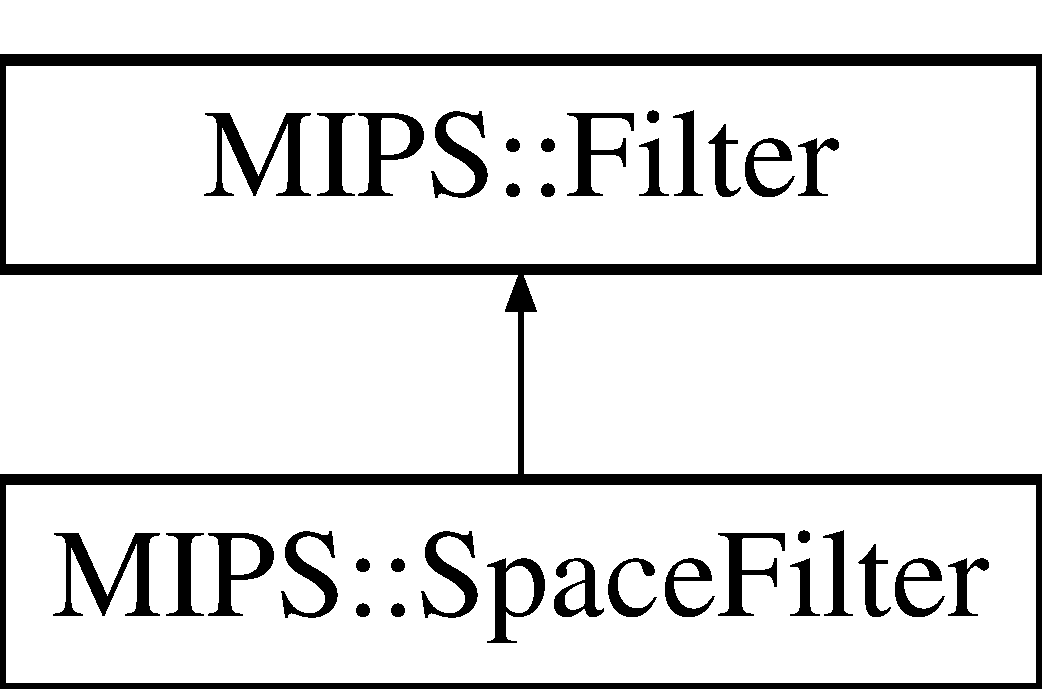
\includegraphics[height=2.000000cm]{classMIPS_1_1SpaceFilter}
\end{center}
\end{figure}
\subsection*{Public Member Functions}
\begin{DoxyCompactItemize}
\item 
std\+::string \hyperlink{classMIPS_1_1SpaceFilter_af6182f9ed8fb061e3ab9d7b437234952}{filter} (std\+::string \&input)
\end{DoxyCompactItemize}


\subsection{Detailed Description}
Classe responsável por remover espaços e tabulações de um texto.

\begin{DoxyAuthor}{Author}
Matheus Matheus Nogueira 
\end{DoxyAuthor}


\subsection{Member Function Documentation}
\index{M\+I\+P\+S\+::\+Space\+Filter@{M\+I\+P\+S\+::\+Space\+Filter}!filter@{filter}}
\index{filter@{filter}!M\+I\+P\+S\+::\+Space\+Filter@{M\+I\+P\+S\+::\+Space\+Filter}}
\subsubsection[{\texorpdfstring{filter(std\+::string \&input)}{filter(std::string &input)}}]{\setlength{\rightskip}{0pt plus 5cm}std\+::string M\+I\+P\+S\+::\+Space\+Filter\+::filter (
\begin{DoxyParamCaption}
\item[{std\+::string \&}]{input}
\end{DoxyParamCaption}
)\hspace{0.3cm}{\ttfamily [virtual]}}\hypertarget{classMIPS_1_1SpaceFilter_af6182f9ed8fb061e3ab9d7b437234952}{}\label{classMIPS_1_1SpaceFilter_af6182f9ed8fb061e3ab9d7b437234952}
Remove todos os espaços e tabulações de uma string.


\begin{DoxyParams}{Parameters}
{\em input} & string a ser filtrada. \\
\hline
\end{DoxyParams}
\begin{DoxyReturn}{Returns}
string filtrada. 
\end{DoxyReturn}


Implements \hyperlink{classMIPS_1_1Filter_a752c258e9d4090dd774fa4e829c95ae1}{M\+I\+P\+S\+::\+Filter}.



The documentation for this class was generated from the following file\+:\begin{DoxyCompactItemize}
\item 
include/mips/util/filter/\hyperlink{space__filter_8hpp}{space\+\_\+filter.\+hpp}\end{DoxyCompactItemize}

\hypertarget{classMIPS_1_1StoreInstruction}{}\section{M\+I\+PS\+:\+:Store\+Instruction Class Reference}
\label{classMIPS_1_1StoreInstruction}\index{M\+I\+P\+S\+::\+Store\+Instruction@{M\+I\+P\+S\+::\+Store\+Instruction}}


{\ttfamily \#include $<$store.\+hpp$>$}

Inheritance diagram for M\+I\+PS\+:\+:Store\+Instruction\+:\begin{figure}[H]
\begin{center}
\leavevmode
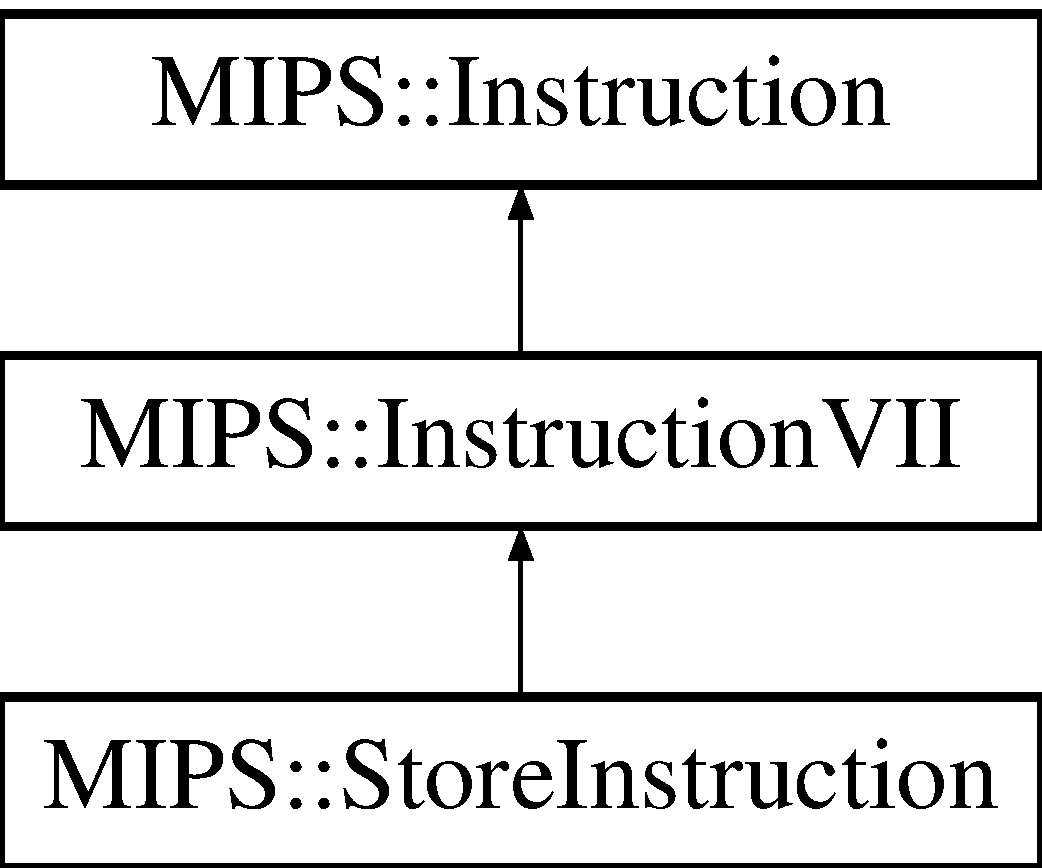
\includegraphics[height=3.000000cm]{classMIPS_1_1StoreInstruction}
\end{center}
\end{figure}
\subsection*{Public Member Functions}
\begin{DoxyCompactItemize}
\item 
\hyperlink{classMIPS_1_1StoreInstruction_ab828ac11fad6c5d8ccf5faca8016232e}{Store\+Instruction} (\hyperlink{core_8hpp_a6074bae122ae7b527864eec42c728c3c}{bit8\+\_\+t} \hyperlink{classMIPS_1_1Instruction_a45cc6808b5dde8a5d41067d148b55476}{opcode}, \hyperlink{classMIPS_1_1Register}{Register} $\ast$\hyperlink{classMIPS_1_1InstructionVII_a8e51202e0b22f8e74668f6de95089e60}{rs}, \hyperlink{classMIPS_1_1Register}{Register} $\ast$\hyperlink{classMIPS_1_1InstructionVII_a8710c06b6e7816f330b0c5daea3402a4}{rt}, \hyperlink{classMIPS_1_1Memory}{Memory} $\ast$\hyperlink{classMIPS_1_1InstructionVII_a4fb34750bedbf137b43f9b55b591e0d7}{memory})
\item 
\hyperlink{core_8hpp_adc265a970bc35995b5879784bbb3f1b7}{bit16\+\_\+t} \hyperlink{classMIPS_1_1StoreInstruction_a8a341407465c275b74c1e067f9dd6459}{execute} ()
\item 
void \hyperlink{classMIPS_1_1StoreInstruction_ab91c709e160c274abd7fe1660cd8fa52}{update\+Control} (\hyperlink{classMIPS_1_1ControlUnit}{Control\+Unit} \&control)
\end{DoxyCompactItemize}
\subsection*{Additional Inherited Members}


\subsection{Detailed Description}
Instrução de Store, carrega na posição da memória endereçada pelo registrador X o conteúdo do registrador Y.

\begin{DoxyAuthor}{Author}
Felipe Dias 
\end{DoxyAuthor}


\subsection{Constructor \& Destructor Documentation}
\index{M\+I\+P\+S\+::\+Store\+Instruction@{M\+I\+P\+S\+::\+Store\+Instruction}!Store\+Instruction@{Store\+Instruction}}
\index{Store\+Instruction@{Store\+Instruction}!M\+I\+P\+S\+::\+Store\+Instruction@{M\+I\+P\+S\+::\+Store\+Instruction}}
\subsubsection[{\texorpdfstring{Store\+Instruction(bit8\+\_\+t opcode, Register $\ast$rs, Register $\ast$rt, Memory $\ast$memory)}{StoreInstruction(bit8_t opcode, Register *rs, Register *rt, Memory *memory)}}]{\setlength{\rightskip}{0pt plus 5cm}M\+I\+P\+S\+::\+Store\+Instruction\+::\+Store\+Instruction (
\begin{DoxyParamCaption}
\item[{{\bf bit8\+\_\+t}}]{opcode, }
\item[{{\bf Register} $\ast$}]{rs, }
\item[{{\bf Register} $\ast$}]{rt, }
\item[{{\bf Memory} $\ast$}]{memory}
\end{DoxyParamCaption}
)\hspace{0.3cm}{\ttfamily [inline]}}\hypertarget{classMIPS_1_1StoreInstruction_ab828ac11fad6c5d8ccf5faca8016232e}{}\label{classMIPS_1_1StoreInstruction_ab828ac11fad6c5d8ccf5faca8016232e}
Constroi uma nova instrução. 

\subsection{Member Function Documentation}
\index{M\+I\+P\+S\+::\+Store\+Instruction@{M\+I\+P\+S\+::\+Store\+Instruction}!execute@{execute}}
\index{execute@{execute}!M\+I\+P\+S\+::\+Store\+Instruction@{M\+I\+P\+S\+::\+Store\+Instruction}}
\subsubsection[{\texorpdfstring{execute()}{execute()}}]{\setlength{\rightskip}{0pt plus 5cm}{\bf bit16\+\_\+t} M\+I\+P\+S\+::\+Store\+Instruction\+::execute (
\begin{DoxyParamCaption}
{}
\end{DoxyParamCaption}
)\hspace{0.3cm}{\ttfamily [virtual]}}\hypertarget{classMIPS_1_1StoreInstruction_a8a341407465c275b74c1e067f9dd6459}{}\label{classMIPS_1_1StoreInstruction_a8a341407465c275b74c1e067f9dd6459}
Executa a instrução.

\begin{DoxyReturn}{Returns}
resultado da instrução 
\end{DoxyReturn}


Implements \hyperlink{classMIPS_1_1InstructionVII_ab004a9cdc0efa7afacb964352abf3ee7}{M\+I\+P\+S\+::\+Instruction\+V\+II}.

\index{M\+I\+P\+S\+::\+Store\+Instruction@{M\+I\+P\+S\+::\+Store\+Instruction}!update\+Control@{update\+Control}}
\index{update\+Control@{update\+Control}!M\+I\+P\+S\+::\+Store\+Instruction@{M\+I\+P\+S\+::\+Store\+Instruction}}
\subsubsection[{\texorpdfstring{update\+Control(\+Control\+Unit \&control)}{updateControl(ControlUnit &control)}}]{\setlength{\rightskip}{0pt plus 5cm}void M\+I\+P\+S\+::\+Store\+Instruction\+::update\+Control (
\begin{DoxyParamCaption}
\item[{{\bf Control\+Unit} \&}]{control}
\end{DoxyParamCaption}
)\hspace{0.3cm}{\ttfamily [inline]}, {\ttfamily [virtual]}}\hypertarget{classMIPS_1_1StoreInstruction_ab91c709e160c274abd7fe1660cd8fa52}{}\label{classMIPS_1_1StoreInstruction_ab91c709e160c274abd7fe1660cd8fa52}
Método utilizado para atualizar os sinais de controle do processador.


\begin{DoxyParams}{Parameters}
{\em control} & unidade de controle do processador. \\
\hline
\end{DoxyParams}


Reimplemented from \hyperlink{classMIPS_1_1Instruction_a7df847adef2997446ffca9b71c2f3112}{M\+I\+P\+S\+::\+Instruction}.



The documentation for this class was generated from the following file\+:\begin{DoxyCompactItemize}
\item 
include/mips/instructions/format\+\_\+\+V\+I\+I/\hyperlink{store_8hpp}{store.\+hpp}\end{DoxyCompactItemize}

\hypertarget{classMIPS_1_1SubdecInstruction}{}\section{M\+I\+PS\+:\+:Subdec\+Instruction Class Reference}
\label{classMIPS_1_1SubdecInstruction}\index{M\+I\+P\+S\+::\+Subdec\+Instruction@{M\+I\+P\+S\+::\+Subdec\+Instruction}}


{\ttfamily \#include $<$subdec.\+hpp$>$}

Inheritance diagram for M\+I\+PS\+:\+:Subdec\+Instruction\+:\begin{figure}[H]
\begin{center}
\leavevmode
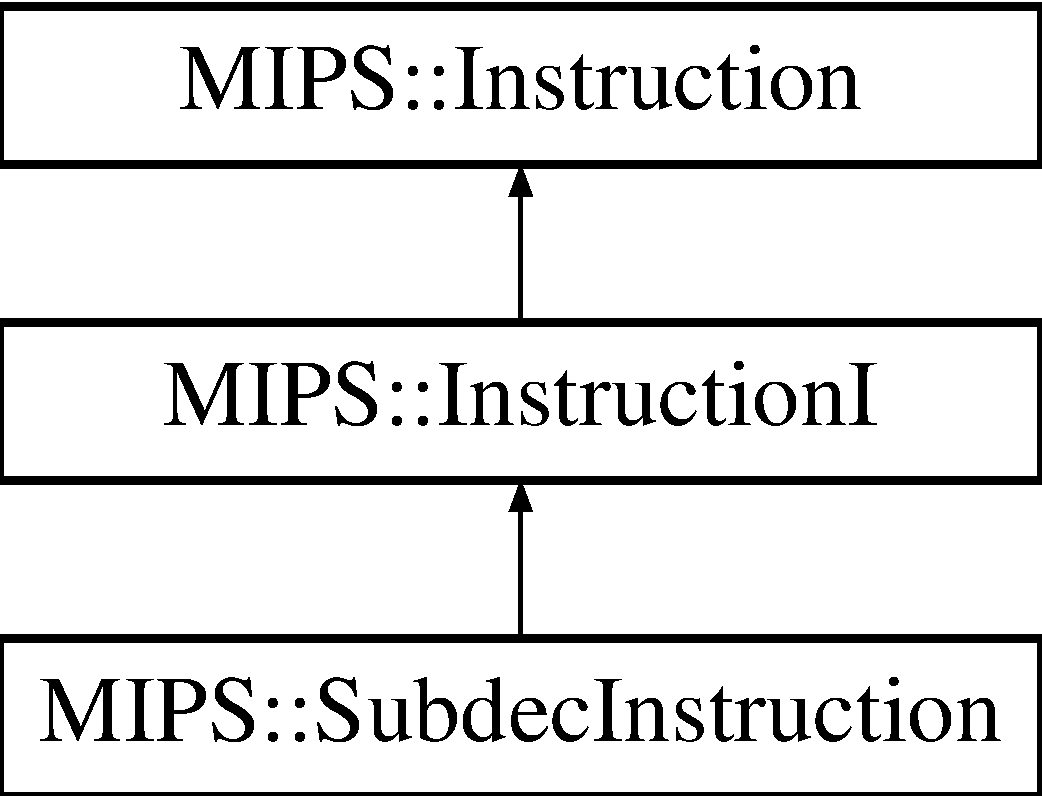
\includegraphics[height=3.000000cm]{classMIPS_1_1SubdecInstruction}
\end{center}
\end{figure}
\subsection*{Public Member Functions}
\begin{DoxyCompactItemize}
\item 
\hyperlink{classMIPS_1_1SubdecInstruction_add4c367579966be84f60cf36d84ae332}{Subdec\+Instruction} (\hyperlink{core_8hpp_a6074bae122ae7b527864eec42c728c3c}{bit8\+\_\+t} \hyperlink{classMIPS_1_1Instruction_a45cc6808b5dde8a5d41067d148b55476}{opcode}, \hyperlink{classMIPS_1_1Register}{Register} $\ast$\hyperlink{classMIPS_1_1InstructionI_a2be191d5b3dce505e2e626ec02eb4d62}{rs}, \hyperlink{classMIPS_1_1Register}{Register} $\ast$\hyperlink{classMIPS_1_1InstructionI_add1db07a5c954f35271de8c8a5737487}{rt}, \hyperlink{core_8hpp_a6074bae122ae7b527864eec42c728c3c}{bit8\+\_\+t} \hyperlink{classMIPS_1_1InstructionI_aa9b6da37c374c2ec8d96448d341e5e7d}{shamt}, \hyperlink{core_8hpp_a6074bae122ae7b527864eec42c728c3c}{bit8\+\_\+t} \hyperlink{classMIPS_1_1InstructionI_a5c6efcbbd233a7447c1fe24ea0a1e558}{funct})
\item 
\hyperlink{core_8hpp_adc265a970bc35995b5879784bbb3f1b7}{bit16\+\_\+t} \hyperlink{classMIPS_1_1SubdecInstruction_a6d9e86774b950a584b60d9a48402af2a}{execute} ()
\end{DoxyCompactItemize}
\subsection*{Additional Inherited Members}


\subsection{Detailed Description}
Classe que faz a operação de subdec no processador.

\begin{DoxyAuthor}{Author}
Lucas Pereira 
\end{DoxyAuthor}


\subsection{Constructor \& Destructor Documentation}
\index{M\+I\+P\+S\+::\+Subdec\+Instruction@{M\+I\+P\+S\+::\+Subdec\+Instruction}!Subdec\+Instruction@{Subdec\+Instruction}}
\index{Subdec\+Instruction@{Subdec\+Instruction}!M\+I\+P\+S\+::\+Subdec\+Instruction@{M\+I\+P\+S\+::\+Subdec\+Instruction}}
\subsubsection[{\texorpdfstring{Subdec\+Instruction(bit8\+\_\+t opcode, Register $\ast$rs, Register $\ast$rt, bit8\+\_\+t shamt, bit8\+\_\+t funct)}{SubdecInstruction(bit8_t opcode, Register *rs, Register *rt, bit8_t shamt, bit8_t funct)}}]{\setlength{\rightskip}{0pt plus 5cm}M\+I\+P\+S\+::\+Subdec\+Instruction\+::\+Subdec\+Instruction (
\begin{DoxyParamCaption}
\item[{{\bf bit8\+\_\+t}}]{opcode, }
\item[{{\bf Register} $\ast$}]{rs, }
\item[{{\bf Register} $\ast$}]{rt, }
\item[{{\bf bit8\+\_\+t}}]{shamt, }
\item[{{\bf bit8\+\_\+t}}]{funct}
\end{DoxyParamCaption}
)\hspace{0.3cm}{\ttfamily [inline]}}\hypertarget{classMIPS_1_1SubdecInstruction_add4c367579966be84f60cf36d84ae332}{}\label{classMIPS_1_1SubdecInstruction_add4c367579966be84f60cf36d84ae332}
Constroi uma nova instrução. 

\subsection{Member Function Documentation}
\index{M\+I\+P\+S\+::\+Subdec\+Instruction@{M\+I\+P\+S\+::\+Subdec\+Instruction}!execute@{execute}}
\index{execute@{execute}!M\+I\+P\+S\+::\+Subdec\+Instruction@{M\+I\+P\+S\+::\+Subdec\+Instruction}}
\subsubsection[{\texorpdfstring{execute()}{execute()}}]{\setlength{\rightskip}{0pt plus 5cm}{\bf bit16\+\_\+t} M\+I\+P\+S\+::\+Subdec\+Instruction\+::execute (
\begin{DoxyParamCaption}
{}
\end{DoxyParamCaption}
)\hspace{0.3cm}{\ttfamily [virtual]}}\hypertarget{classMIPS_1_1SubdecInstruction_a6d9e86774b950a584b60d9a48402af2a}{}\label{classMIPS_1_1SubdecInstruction_a6d9e86774b950a584b60d9a48402af2a}
Função que executa a operação de subtração. 

Implements \hyperlink{classMIPS_1_1InstructionI_ae60fca5801bf5415cdff06d2aa11764f}{M\+I\+P\+S\+::\+InstructionI}.



The documentation for this class was generated from the following file\+:\begin{DoxyCompactItemize}
\item 
include/mips/instructions/format\+\_\+\+I/\hyperlink{subdec_8hpp}{subdec.\+hpp}\end{DoxyCompactItemize}

\hypertarget{classMIPS_1_1SubInstruction}{}\section{M\+I\+PS\+:\+:Sub\+Instruction Class Reference}
\label{classMIPS_1_1SubInstruction}\index{M\+I\+P\+S\+::\+Sub\+Instruction@{M\+I\+P\+S\+::\+Sub\+Instruction}}


{\ttfamily \#include $<$sub.\+hpp$>$}

Inheritance diagram for M\+I\+PS\+:\+:Sub\+Instruction\+:\begin{figure}[H]
\begin{center}
\leavevmode
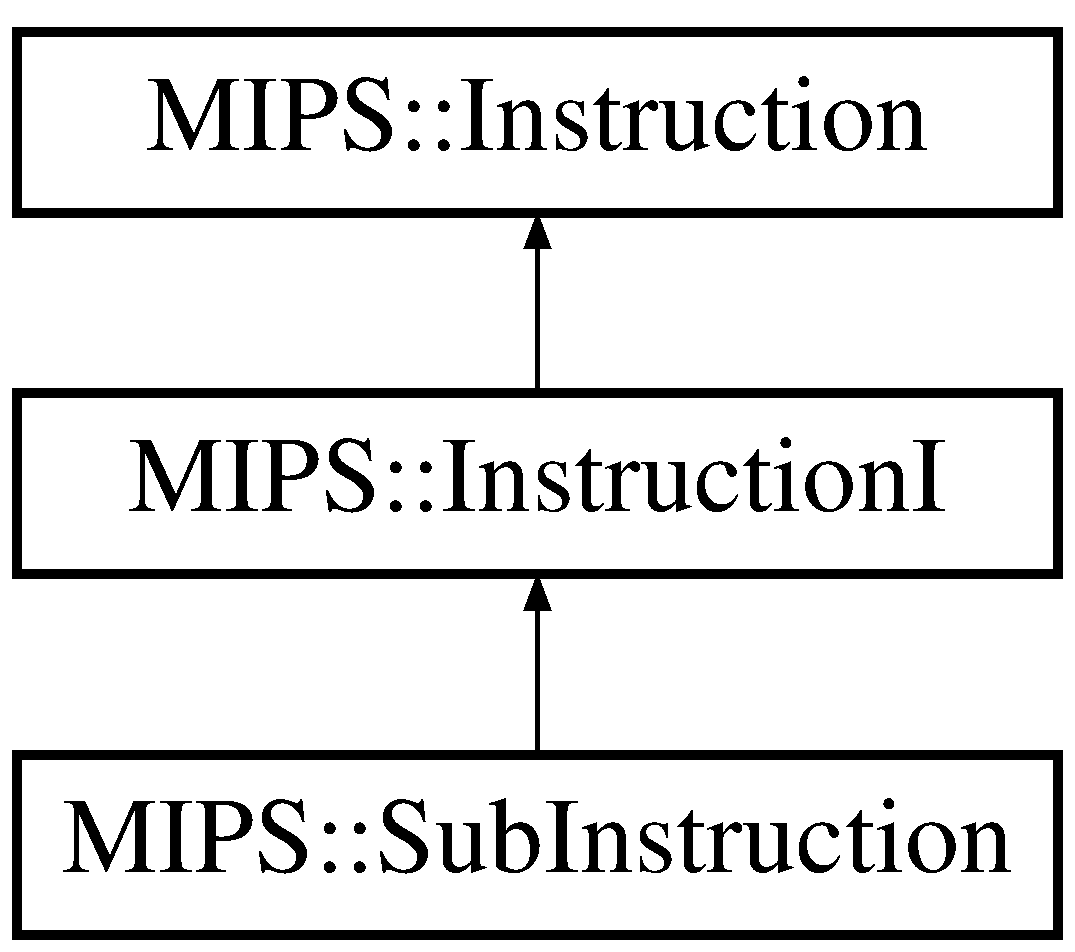
\includegraphics[height=3.000000cm]{classMIPS_1_1SubInstruction}
\end{center}
\end{figure}
\subsection*{Public Member Functions}
\begin{DoxyCompactItemize}
\item 
\hyperlink{classMIPS_1_1SubInstruction_af6979540068224336b460cb680690ecf}{Sub\+Instruction} (\hyperlink{core_8hpp_a6074bae122ae7b527864eec42c728c3c}{bit8\+\_\+t} \hyperlink{classMIPS_1_1Instruction_a45cc6808b5dde8a5d41067d148b55476}{opcode}, \hyperlink{classMIPS_1_1Register}{Register} $\ast$\hyperlink{classMIPS_1_1InstructionI_a2be191d5b3dce505e2e626ec02eb4d62}{rs}, \hyperlink{classMIPS_1_1Register}{Register} $\ast$\hyperlink{classMIPS_1_1InstructionI_add1db07a5c954f35271de8c8a5737487}{rt}, \hyperlink{core_8hpp_a6074bae122ae7b527864eec42c728c3c}{bit8\+\_\+t} \hyperlink{classMIPS_1_1InstructionI_aa9b6da37c374c2ec8d96448d341e5e7d}{shamt}, \hyperlink{core_8hpp_a6074bae122ae7b527864eec42c728c3c}{bit8\+\_\+t} \hyperlink{classMIPS_1_1InstructionI_a5c6efcbbd233a7447c1fe24ea0a1e558}{funct})
\item 
\hyperlink{core_8hpp_adc265a970bc35995b5879784bbb3f1b7}{bit16\+\_\+t} \hyperlink{classMIPS_1_1SubInstruction_a2b10f6bfda0e7d9651600b530cfccf62}{execute} ()
\end{DoxyCompactItemize}
\subsection*{Additional Inherited Members}


\subsection{Detailed Description}
Classe que faz a operação de A\+DD no processador.

\begin{DoxyAuthor}{Author}
Felipe Dias 
\end{DoxyAuthor}


\subsection{Constructor \& Destructor Documentation}
\index{M\+I\+P\+S\+::\+Sub\+Instruction@{M\+I\+P\+S\+::\+Sub\+Instruction}!Sub\+Instruction@{Sub\+Instruction}}
\index{Sub\+Instruction@{Sub\+Instruction}!M\+I\+P\+S\+::\+Sub\+Instruction@{M\+I\+P\+S\+::\+Sub\+Instruction}}
\subsubsection[{\texorpdfstring{Sub\+Instruction(bit8\+\_\+t opcode, Register $\ast$rs, Register $\ast$rt, bit8\+\_\+t shamt, bit8\+\_\+t funct)}{SubInstruction(bit8_t opcode, Register *rs, Register *rt, bit8_t shamt, bit8_t funct)}}]{\setlength{\rightskip}{0pt plus 5cm}M\+I\+P\+S\+::\+Sub\+Instruction\+::\+Sub\+Instruction (
\begin{DoxyParamCaption}
\item[{{\bf bit8\+\_\+t}}]{opcode, }
\item[{{\bf Register} $\ast$}]{rs, }
\item[{{\bf Register} $\ast$}]{rt, }
\item[{{\bf bit8\+\_\+t}}]{shamt, }
\item[{{\bf bit8\+\_\+t}}]{funct}
\end{DoxyParamCaption}
)\hspace{0.3cm}{\ttfamily [inline]}}\hypertarget{classMIPS_1_1SubInstruction_af6979540068224336b460cb680690ecf}{}\label{classMIPS_1_1SubInstruction_af6979540068224336b460cb680690ecf}
Constroi uma nova instrução. 

\subsection{Member Function Documentation}
\index{M\+I\+P\+S\+::\+Sub\+Instruction@{M\+I\+P\+S\+::\+Sub\+Instruction}!execute@{execute}}
\index{execute@{execute}!M\+I\+P\+S\+::\+Sub\+Instruction@{M\+I\+P\+S\+::\+Sub\+Instruction}}
\subsubsection[{\texorpdfstring{execute()}{execute()}}]{\setlength{\rightskip}{0pt plus 5cm}{\bf bit16\+\_\+t} M\+I\+P\+S\+::\+Sub\+Instruction\+::execute (
\begin{DoxyParamCaption}
{}
\end{DoxyParamCaption}
)\hspace{0.3cm}{\ttfamily [virtual]}}\hypertarget{classMIPS_1_1SubInstruction_a2b10f6bfda0e7d9651600b530cfccf62}{}\label{classMIPS_1_1SubInstruction_a2b10f6bfda0e7d9651600b530cfccf62}
Função que executa a operação de soma.

\begin{DoxyReturn}{Returns}
resultado da operação 
\end{DoxyReturn}


Implements \hyperlink{classMIPS_1_1InstructionI_ae60fca5801bf5415cdff06d2aa11764f}{M\+I\+P\+S\+::\+InstructionI}.



The documentation for this class was generated from the following file\+:\begin{DoxyCompactItemize}
\item 
include/mips/instructions/format\+\_\+\+I/sub.\+hpp\end{DoxyCompactItemize}

\hypertarget{classMIPS_1_1Tokenizer}{}\section{M\+I\+PS\+:\+:Tokenizer Class Reference}
\label{classMIPS_1_1Tokenizer}\index{M\+I\+P\+S\+::\+Tokenizer@{M\+I\+P\+S\+::\+Tokenizer}}


{\ttfamily \#include $<$tokenizer.\+hpp$>$}

\subsection*{Public Member Functions}
\begin{DoxyCompactItemize}
\item 
void \hyperlink{classMIPS_1_1Tokenizer_a928c83ccd97fc9b5ef16864ab1b90e1f}{tokenize} (char $\ast$str, std\+::vector$<$ char $\ast$ $>$ \&vector)
\end{DoxyCompactItemize}


\subsection{Detailed Description}
Classe responsável por quebrar uma string em diversos tokens.

\begin{DoxyAuthor}{Author}
Matheus Nogueira 
\end{DoxyAuthor}


\subsection{Member Function Documentation}
\index{M\+I\+P\+S\+::\+Tokenizer@{M\+I\+P\+S\+::\+Tokenizer}!tokenize@{tokenize}}
\index{tokenize@{tokenize}!M\+I\+P\+S\+::\+Tokenizer@{M\+I\+P\+S\+::\+Tokenizer}}
\subsubsection[{\texorpdfstring{tokenize(char $\ast$str, std\+::vector$<$ char $\ast$ $>$ \&vector)}{tokenize(char *str, std::vector< char * > &vector)}}]{\setlength{\rightskip}{0pt plus 5cm}void M\+I\+P\+S\+::\+Tokenizer\+::tokenize (
\begin{DoxyParamCaption}
\item[{char $\ast$}]{str, }
\item[{std\+::vector$<$ char $\ast$ $>$ \&}]{vector}
\end{DoxyParamCaption}
)}\hypertarget{classMIPS_1_1Tokenizer_a928c83ccd97fc9b5ef16864ab1b90e1f}{}\label{classMIPS_1_1Tokenizer_a928c83ccd97fc9b5ef16864ab1b90e1f}
Retira os tokens de uma string e os armazena em um vector.


\begin{DoxyParams}{Parameters}
{\em str} & string contendo os tokens \\
\hline
{\em vector} & vector que será usado para armazenar os tokens \\
\hline
\end{DoxyParams}


The documentation for this class was generated from the following file\+:\begin{DoxyCompactItemize}
\item 
include/mips/interpreter/parser/\hyperlink{tokenizer_8hpp}{tokenizer.\+hpp}\end{DoxyCompactItemize}

\hypertarget{classMIPS_1_1XnorInstruction}{}\section{M\+I\+PS\+:\+:Xnor\+Instruction Class Reference}
\label{classMIPS_1_1XnorInstruction}\index{M\+I\+P\+S\+::\+Xnor\+Instruction@{M\+I\+P\+S\+::\+Xnor\+Instruction}}


{\ttfamily \#include $<$xnor.\+hpp$>$}

Inheritance diagram for M\+I\+PS\+:\+:Xnor\+Instruction\+:\begin{figure}[H]
\begin{center}
\leavevmode
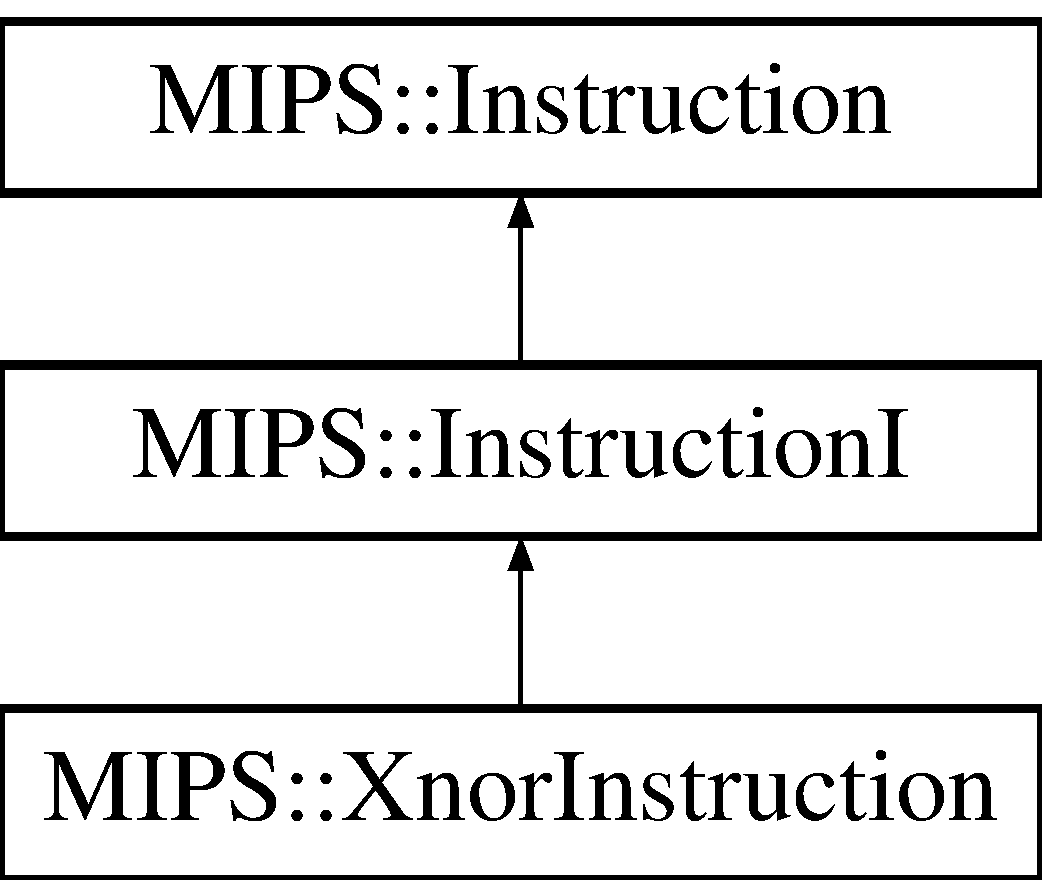
\includegraphics[height=3.000000cm]{classMIPS_1_1XnorInstruction}
\end{center}
\end{figure}
\subsection*{Public Member Functions}
\begin{DoxyCompactItemize}
\item 
\hyperlink{classMIPS_1_1XnorInstruction_aa6ace56cbc1f0a87f0661ecf5925bc2d}{Xnor\+Instruction} (\hyperlink{core_8hpp_a6074bae122ae7b527864eec42c728c3c}{bit8\+\_\+t} \hyperlink{classMIPS_1_1Instruction_a45cc6808b5dde8a5d41067d148b55476}{opcode}, \hyperlink{classMIPS_1_1Register}{Register} $\ast$\hyperlink{classMIPS_1_1InstructionI_a2be191d5b3dce505e2e626ec02eb4d62}{rs}, \hyperlink{classMIPS_1_1Register}{Register} $\ast$\hyperlink{classMIPS_1_1InstructionI_add1db07a5c954f35271de8c8a5737487}{rt}, \hyperlink{core_8hpp_a6074bae122ae7b527864eec42c728c3c}{bit8\+\_\+t} \hyperlink{classMIPS_1_1InstructionI_aa9b6da37c374c2ec8d96448d341e5e7d}{shamt}, \hyperlink{core_8hpp_a6074bae122ae7b527864eec42c728c3c}{bit8\+\_\+t} \hyperlink{classMIPS_1_1InstructionI_a5c6efcbbd233a7447c1fe24ea0a1e558}{funct})
\item 
\hyperlink{core_8hpp_adc265a970bc35995b5879784bbb3f1b7}{bit16\+\_\+t} \hyperlink{classMIPS_1_1XnorInstruction_a4b5ae9a875883902c0ed1e237e753f31}{execute} ()
\end{DoxyCompactItemize}
\subsection*{Additional Inherited Members}


\subsection{Detailed Description}
Classe que faz a operação de X\+N\+OR no processador.

\begin{DoxyAuthor}{Author}
Matheus Nogueira 
\end{DoxyAuthor}


\subsection{Constructor \& Destructor Documentation}
\index{M\+I\+P\+S\+::\+Xnor\+Instruction@{M\+I\+P\+S\+::\+Xnor\+Instruction}!Xnor\+Instruction@{Xnor\+Instruction}}
\index{Xnor\+Instruction@{Xnor\+Instruction}!M\+I\+P\+S\+::\+Xnor\+Instruction@{M\+I\+P\+S\+::\+Xnor\+Instruction}}
\subsubsection[{\texorpdfstring{Xnor\+Instruction(bit8\+\_\+t opcode, Register $\ast$rs, Register $\ast$rt, bit8\+\_\+t shamt, bit8\+\_\+t funct)}{XnorInstruction(bit8_t opcode, Register *rs, Register *rt, bit8_t shamt, bit8_t funct)}}]{\setlength{\rightskip}{0pt plus 5cm}M\+I\+P\+S\+::\+Xnor\+Instruction\+::\+Xnor\+Instruction (
\begin{DoxyParamCaption}
\item[{{\bf bit8\+\_\+t}}]{opcode, }
\item[{{\bf Register} $\ast$}]{rs, }
\item[{{\bf Register} $\ast$}]{rt, }
\item[{{\bf bit8\+\_\+t}}]{shamt, }
\item[{{\bf bit8\+\_\+t}}]{funct}
\end{DoxyParamCaption}
)\hspace{0.3cm}{\ttfamily [inline]}}\hypertarget{classMIPS_1_1XnorInstruction_aa6ace56cbc1f0a87f0661ecf5925bc2d}{}\label{classMIPS_1_1XnorInstruction_aa6ace56cbc1f0a87f0661ecf5925bc2d}
Constroi uma nova instrução. 

\subsection{Member Function Documentation}
\index{M\+I\+P\+S\+::\+Xnor\+Instruction@{M\+I\+P\+S\+::\+Xnor\+Instruction}!execute@{execute}}
\index{execute@{execute}!M\+I\+P\+S\+::\+Xnor\+Instruction@{M\+I\+P\+S\+::\+Xnor\+Instruction}}
\subsubsection[{\texorpdfstring{execute()}{execute()}}]{\setlength{\rightskip}{0pt plus 5cm}{\bf bit16\+\_\+t} M\+I\+P\+S\+::\+Xnor\+Instruction\+::execute (
\begin{DoxyParamCaption}
{}
\end{DoxyParamCaption}
)\hspace{0.3cm}{\ttfamily [virtual]}}\hypertarget{classMIPS_1_1XnorInstruction_a4b5ae9a875883902c0ed1e237e753f31}{}\label{classMIPS_1_1XnorInstruction_a4b5ae9a875883902c0ed1e237e753f31}
Função que executa a operação de soma.

\begin{DoxyReturn}{Returns}
resultado da operação 
\end{DoxyReturn}


Implements \hyperlink{classMIPS_1_1InstructionI_ae60fca5801bf5415cdff06d2aa11764f}{M\+I\+P\+S\+::\+InstructionI}.



The documentation for this class was generated from the following file\+:\begin{DoxyCompactItemize}
\item 
include/mips/instructions/format\+\_\+\+I/\hyperlink{xnor_8hpp}{xnor.\+hpp}\end{DoxyCompactItemize}

\hypertarget{classMIPS_1_1XorInstruction}{}\section{M\+I\+PS\+:\+:Xor\+Instruction Class Reference}
\label{classMIPS_1_1XorInstruction}\index{M\+I\+P\+S\+::\+Xor\+Instruction@{M\+I\+P\+S\+::\+Xor\+Instruction}}


{\ttfamily \#include $<$xor.\+hpp$>$}

Inheritance diagram for M\+I\+PS\+:\+:Xor\+Instruction\+:\begin{figure}[H]
\begin{center}
\leavevmode
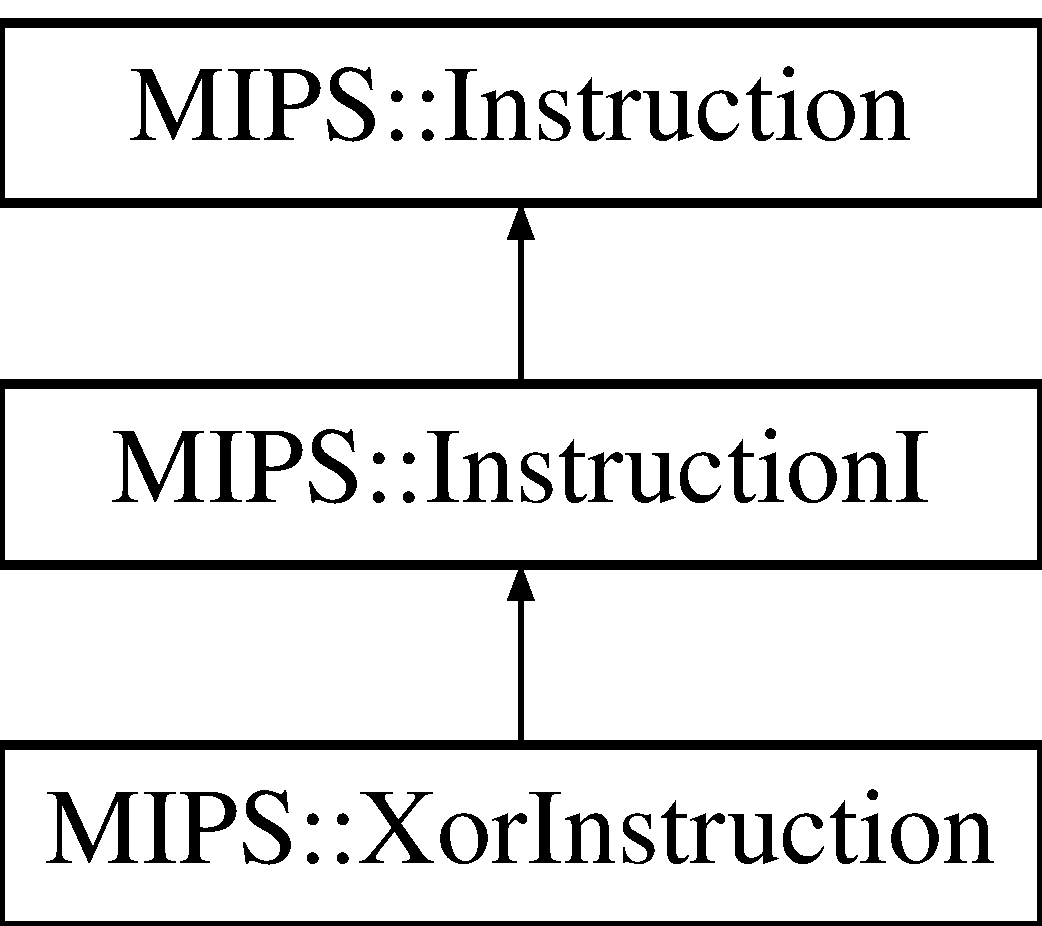
\includegraphics[height=3.000000cm]{classMIPS_1_1XorInstruction}
\end{center}
\end{figure}
\subsection*{Public Member Functions}
\begin{DoxyCompactItemize}
\item 
\hyperlink{classMIPS_1_1XorInstruction_ac6b0e810912319f45b0e42b80d9b0f9e}{Xor\+Instruction} (\hyperlink{core_8hpp_a6074bae122ae7b527864eec42c728c3c}{bit8\+\_\+t} \hyperlink{classMIPS_1_1Instruction_a45cc6808b5dde8a5d41067d148b55476}{opcode}, \hyperlink{classMIPS_1_1Register}{Register} $\ast$\hyperlink{classMIPS_1_1InstructionI_a2be191d5b3dce505e2e626ec02eb4d62}{rs}, \hyperlink{classMIPS_1_1Register}{Register} $\ast$\hyperlink{classMIPS_1_1InstructionI_add1db07a5c954f35271de8c8a5737487}{rt}, \hyperlink{core_8hpp_a6074bae122ae7b527864eec42c728c3c}{bit8\+\_\+t} \hyperlink{classMIPS_1_1InstructionI_aa9b6da37c374c2ec8d96448d341e5e7d}{shamt}, \hyperlink{core_8hpp_a6074bae122ae7b527864eec42c728c3c}{bit8\+\_\+t} \hyperlink{classMIPS_1_1InstructionI_a5c6efcbbd233a7447c1fe24ea0a1e558}{funct})
\item 
\hyperlink{core_8hpp_adc265a970bc35995b5879784bbb3f1b7}{bit16\+\_\+t} \hyperlink{classMIPS_1_1XorInstruction_aaebc7dc8723627871ba2caf85f01fbea}{execute} ()
\end{DoxyCompactItemize}
\subsection*{Additional Inherited Members}


\subsection{Detailed Description}
Classe que faz a operação de X\+OR no processador.

\begin{DoxyAuthor}{Author}
Felipe Dias 
\end{DoxyAuthor}


\subsection{Constructor \& Destructor Documentation}
\index{M\+I\+P\+S\+::\+Xor\+Instruction@{M\+I\+P\+S\+::\+Xor\+Instruction}!Xor\+Instruction@{Xor\+Instruction}}
\index{Xor\+Instruction@{Xor\+Instruction}!M\+I\+P\+S\+::\+Xor\+Instruction@{M\+I\+P\+S\+::\+Xor\+Instruction}}
\subsubsection[{\texorpdfstring{Xor\+Instruction(bit8\+\_\+t opcode, Register $\ast$rs, Register $\ast$rt, bit8\+\_\+t shamt, bit8\+\_\+t funct)}{XorInstruction(bit8_t opcode, Register *rs, Register *rt, bit8_t shamt, bit8_t funct)}}]{\setlength{\rightskip}{0pt plus 5cm}M\+I\+P\+S\+::\+Xor\+Instruction\+::\+Xor\+Instruction (
\begin{DoxyParamCaption}
\item[{{\bf bit8\+\_\+t}}]{opcode, }
\item[{{\bf Register} $\ast$}]{rs, }
\item[{{\bf Register} $\ast$}]{rt, }
\item[{{\bf bit8\+\_\+t}}]{shamt, }
\item[{{\bf bit8\+\_\+t}}]{funct}
\end{DoxyParamCaption}
)\hspace{0.3cm}{\ttfamily [inline]}}\hypertarget{classMIPS_1_1XorInstruction_ac6b0e810912319f45b0e42b80d9b0f9e}{}\label{classMIPS_1_1XorInstruction_ac6b0e810912319f45b0e42b80d9b0f9e}
Constroi uma nova instrução. 

\subsection{Member Function Documentation}
\index{M\+I\+P\+S\+::\+Xor\+Instruction@{M\+I\+P\+S\+::\+Xor\+Instruction}!execute@{execute}}
\index{execute@{execute}!M\+I\+P\+S\+::\+Xor\+Instruction@{M\+I\+P\+S\+::\+Xor\+Instruction}}
\subsubsection[{\texorpdfstring{execute()}{execute()}}]{\setlength{\rightskip}{0pt plus 5cm}{\bf bit16\+\_\+t} M\+I\+P\+S\+::\+Xor\+Instruction\+::execute (
\begin{DoxyParamCaption}
{}
\end{DoxyParamCaption}
)\hspace{0.3cm}{\ttfamily [virtual]}}\hypertarget{classMIPS_1_1XorInstruction_aaebc7dc8723627871ba2caf85f01fbea}{}\label{classMIPS_1_1XorInstruction_aaebc7dc8723627871ba2caf85f01fbea}
Função que executa a operação de soma.

\begin{DoxyReturn}{Returns}
resultado da operação 
\end{DoxyReturn}


Implements \hyperlink{classMIPS_1_1InstructionI_ae60fca5801bf5415cdff06d2aa11764f}{M\+I\+P\+S\+::\+InstructionI}.



The documentation for this class was generated from the following file\+:\begin{DoxyCompactItemize}
\item 
include/mips/instructions/format\+\_\+\+I/\hyperlink{xor_8hpp}{xor.\+hpp}\end{DoxyCompactItemize}

\hypertarget{classMIPS_1_1ZeroInstruction}{}\section{M\+I\+PS\+:\+:Zero\+Instruction Class Reference}
\label{classMIPS_1_1ZeroInstruction}\index{M\+I\+P\+S\+::\+Zero\+Instruction@{M\+I\+P\+S\+::\+Zero\+Instruction}}


{\ttfamily \#include $<$zero.\+hpp$>$}

Inheritance diagram for M\+I\+PS\+:\+:Zero\+Instruction\+:\begin{figure}[H]
\begin{center}
\leavevmode
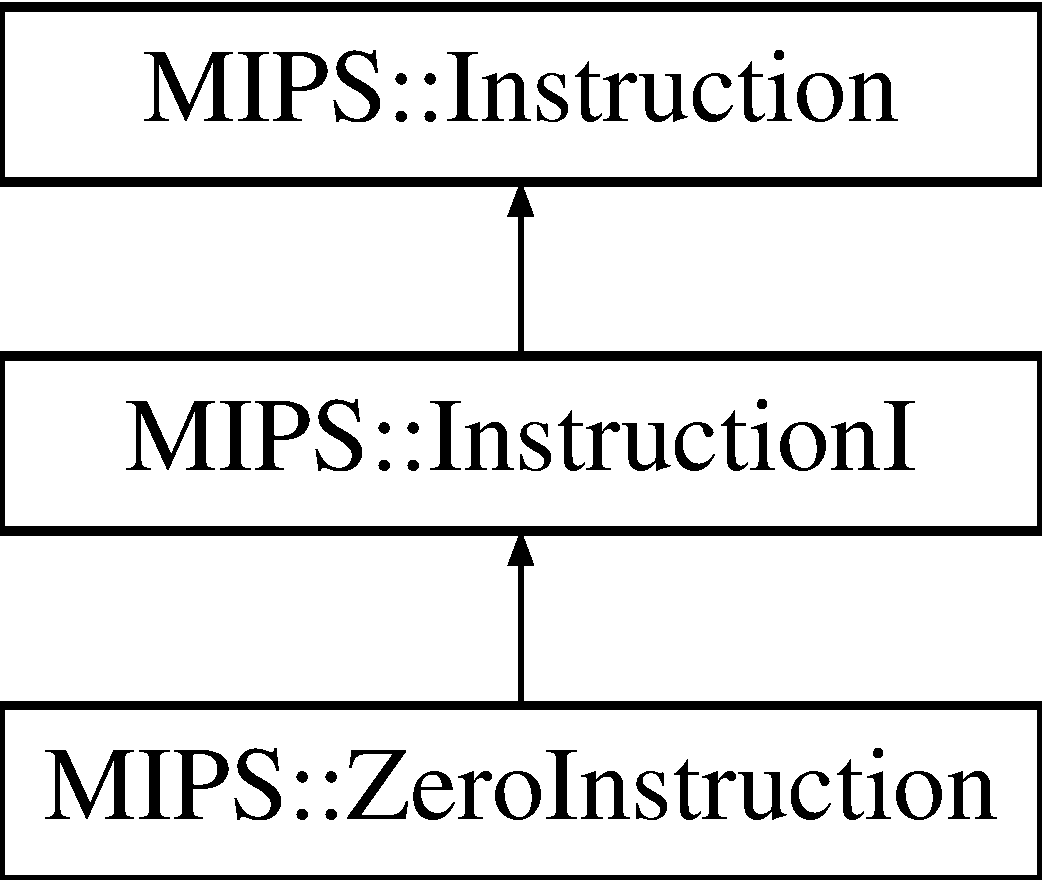
\includegraphics[height=3.000000cm]{classMIPS_1_1ZeroInstruction}
\end{center}
\end{figure}
\subsection*{Public Member Functions}
\begin{DoxyCompactItemize}
\item 
\hyperlink{classMIPS_1_1ZeroInstruction_ac8e066062f919823b60900d2f3e23348}{Zero\+Instruction} (\hyperlink{core_8hpp_a6074bae122ae7b527864eec42c728c3c}{bit8\+\_\+t} \hyperlink{classMIPS_1_1Instruction_a45cc6808b5dde8a5d41067d148b55476}{opcode}, \hyperlink{classMIPS_1_1Register}{Register} $\ast$\hyperlink{classMIPS_1_1InstructionI_a2be191d5b3dce505e2e626ec02eb4d62}{rs}, \hyperlink{classMIPS_1_1Register}{Register} $\ast$\hyperlink{classMIPS_1_1InstructionI_add1db07a5c954f35271de8c8a5737487}{rt}, \hyperlink{core_8hpp_a6074bae122ae7b527864eec42c728c3c}{bit8\+\_\+t} \hyperlink{classMIPS_1_1InstructionI_aa9b6da37c374c2ec8d96448d341e5e7d}{shamt}, \hyperlink{core_8hpp_a6074bae122ae7b527864eec42c728c3c}{bit8\+\_\+t} \hyperlink{classMIPS_1_1InstructionI_a5c6efcbbd233a7447c1fe24ea0a1e558}{funct})
\item 
\hyperlink{core_8hpp_adc265a970bc35995b5879784bbb3f1b7}{bit16\+\_\+t} \hyperlink{classMIPS_1_1ZeroInstruction_a9596a96b4bf7a51672ab14386d111bad}{execute} ()
\end{DoxyCompactItemize}
\subsection*{Additional Inherited Members}


\subsection{Detailed Description}
Classe que faz a operação de Z\+E\+RO no processador.

\begin{DoxyAuthor}{Author}
Felipe Dias 
\end{DoxyAuthor}


\subsection{Constructor \& Destructor Documentation}
\index{M\+I\+P\+S\+::\+Zero\+Instruction@{M\+I\+P\+S\+::\+Zero\+Instruction}!Zero\+Instruction@{Zero\+Instruction}}
\index{Zero\+Instruction@{Zero\+Instruction}!M\+I\+P\+S\+::\+Zero\+Instruction@{M\+I\+P\+S\+::\+Zero\+Instruction}}
\subsubsection[{\texorpdfstring{Zero\+Instruction(bit8\+\_\+t opcode, Register $\ast$rs, Register $\ast$rt, bit8\+\_\+t shamt, bit8\+\_\+t funct)}{ZeroInstruction(bit8_t opcode, Register *rs, Register *rt, bit8_t shamt, bit8_t funct)}}]{\setlength{\rightskip}{0pt plus 5cm}M\+I\+P\+S\+::\+Zero\+Instruction\+::\+Zero\+Instruction (
\begin{DoxyParamCaption}
\item[{{\bf bit8\+\_\+t}}]{opcode, }
\item[{{\bf Register} $\ast$}]{rs, }
\item[{{\bf Register} $\ast$}]{rt, }
\item[{{\bf bit8\+\_\+t}}]{shamt, }
\item[{{\bf bit8\+\_\+t}}]{funct}
\end{DoxyParamCaption}
)\hspace{0.3cm}{\ttfamily [inline]}}\hypertarget{classMIPS_1_1ZeroInstruction_ac8e066062f919823b60900d2f3e23348}{}\label{classMIPS_1_1ZeroInstruction_ac8e066062f919823b60900d2f3e23348}
Constroi uma nova instrução. 

\subsection{Member Function Documentation}
\index{M\+I\+P\+S\+::\+Zero\+Instruction@{M\+I\+P\+S\+::\+Zero\+Instruction}!execute@{execute}}
\index{execute@{execute}!M\+I\+P\+S\+::\+Zero\+Instruction@{M\+I\+P\+S\+::\+Zero\+Instruction}}
\subsubsection[{\texorpdfstring{execute()}{execute()}}]{\setlength{\rightskip}{0pt plus 5cm}{\bf bit16\+\_\+t} M\+I\+P\+S\+::\+Zero\+Instruction\+::execute (
\begin{DoxyParamCaption}
{}
\end{DoxyParamCaption}
)\hspace{0.3cm}{\ttfamily [virtual]}}\hypertarget{classMIPS_1_1ZeroInstruction_a9596a96b4bf7a51672ab14386d111bad}{}\label{classMIPS_1_1ZeroInstruction_a9596a96b4bf7a51672ab14386d111bad}
Função que executa a operação de soma.

\begin{DoxyReturn}{Returns}
resultado da operação 
\end{DoxyReturn}


Implements \hyperlink{classMIPS_1_1InstructionI_ae60fca5801bf5415cdff06d2aa11764f}{M\+I\+P\+S\+::\+InstructionI}.



The documentation for this class was generated from the following file\+:\begin{DoxyCompactItemize}
\item 
include/mips/instructions/format\+\_\+\+I/\hyperlink{zero_8hpp}{zero.\+hpp}\end{DoxyCompactItemize}

\chapter{File Documentation}
\hypertarget{full__adder_8hpp}{}\section{include/mips/circuits/full\+\_\+adder.hpp File Reference}
\label{full__adder_8hpp}\index{include/mips/circuits/full\+\_\+adder.\+hpp@{include/mips/circuits/full\+\_\+adder.\+hpp}}
{\ttfamily \#include $<$mips/core.\+hpp$>$}\\*
\subsection*{Classes}
\begin{DoxyCompactItemize}
\item 
class \hyperlink{classMIPS_1_1FullAdder}{M\+I\+P\+S\+::\+Full\+Adder}
\end{DoxyCompactItemize}


\subsection{Detailed Description}
Somador de 16 bits. Referencia\+: \href{http://isweb.redwoods.edu/instruct/calderwoodd/diglogic/full.htm}{\tt http\+://isweb.\+redwoods.\+edu/instruct/calderwoodd/diglogic/full.\+htm} 
\hypertarget{signal__extender_8hpp}{}\section{include/mips/circuits/signal\+\_\+extender.hpp File Reference}
\label{signal__extender_8hpp}\index{include/mips/circuits/signal\+\_\+extender.\+hpp@{include/mips/circuits/signal\+\_\+extender.\+hpp}}
{\ttfamily \#include $<$mips/core.\+hpp$>$}\\*
\subsection*{Classes}
\begin{DoxyCompactItemize}
\item 
class \hyperlink{classMIPS_1_1SignalExtender}{M\+I\+P\+S\+::\+Signal\+Extender}
\end{DoxyCompactItemize}


\subsection{Detailed Description}
Estensor de sinal. Converte um número para 16 bits. 
\hypertarget{signal__inversor_8hpp}{}\section{include/mips/circuits/signal\+\_\+inversor.hpp File Reference}
\label{signal__inversor_8hpp}\index{include/mips/circuits/signal\+\_\+inversor.\+hpp@{include/mips/circuits/signal\+\_\+inversor.\+hpp}}
{\ttfamily \#include $<$mips/core.\+hpp$>$}\\*
\subsection*{Classes}
\begin{DoxyCompactItemize}
\item 
class \hyperlink{classMIPS_1_1SignalInversor}{M\+I\+P\+S\+::\+Signal\+Inversor}
\end{DoxyCompactItemize}


\subsection{Detailed Description}
Inversor de sinal em números que utilizam a representação de complemento de 2. 
\hypertarget{core_8hpp}{}\section{include/mips/core.hpp File Reference}
\label{core_8hpp}\index{include/mips/core.\+hpp@{include/mips/core.\+hpp}}
{\ttfamily \#include $<$mips/debug.\+hpp$>$}\\*
\subsection*{Typedefs}
\begin{DoxyCompactItemize}
\item 
typedef signed char \hyperlink{core_8hpp_a6074bae122ae7b527864eec42c728c3c}{M\+I\+P\+S\+::bit8\+\_\+t}
\item 
typedef signed short \hyperlink{core_8hpp_adc265a970bc35995b5879784bbb3f1b7}{M\+I\+P\+S\+::bit16\+\_\+t}
\item 
typedef signed int \hyperlink{core_8hpp_ad5f4c6ca614f67be232930e0e31b9ccc}{M\+I\+P\+S\+::bit32\+\_\+t}
\item 
typedef bit16\+\_\+t \hyperlink{core_8hpp_aa514fd240a0e29abb2a2e4c805d7f1a4}{M\+I\+P\+S\+::instruction\+\_\+t}
\end{DoxyCompactItemize}


\subsection{Detailed Description}
Arquivo que contém tipos utilizados pelo emulaodr. 

\subsection{Typedef Documentation}
\index{core.\+hpp@{core.\+hpp}!bit16\+\_\+t@{bit16\+\_\+t}}
\index{bit16\+\_\+t@{bit16\+\_\+t}!core.\+hpp@{core.\+hpp}}
\subsubsection[{\texorpdfstring{bit16\+\_\+t}{bit16_t}}]{\setlength{\rightskip}{0pt plus 5cm}typedef signed short {\bf M\+I\+P\+S\+::bit16\+\_\+t}}\hypertarget{core_8hpp_file_adc265a970bc35995b5879784bbb3f1b7}{}\label{core_8hpp_file_adc265a970bc35995b5879784bbb3f1b7}
Tipo que representa um inteiro de 16 bits. \index{core.\+hpp@{core.\+hpp}!bit32\+\_\+t@{bit32\+\_\+t}}
\index{bit32\+\_\+t@{bit32\+\_\+t}!core.\+hpp@{core.\+hpp}}
\subsubsection[{\texorpdfstring{bit32\+\_\+t}{bit32_t}}]{\setlength{\rightskip}{0pt plus 5cm}typedef signed int {\bf M\+I\+P\+S\+::bit32\+\_\+t}}\hypertarget{core_8hpp_file_ad5f4c6ca614f67be232930e0e31b9ccc}{}\label{core_8hpp_file_ad5f4c6ca614f67be232930e0e31b9ccc}
Tipo que representa um inteiro de 16 bits. \index{core.\+hpp@{core.\+hpp}!bit8\+\_\+t@{bit8\+\_\+t}}
\index{bit8\+\_\+t@{bit8\+\_\+t}!core.\+hpp@{core.\+hpp}}
\subsubsection[{\texorpdfstring{bit8\+\_\+t}{bit8_t}}]{\setlength{\rightskip}{0pt plus 5cm}typedef signed char {\bf M\+I\+P\+S\+::bit8\+\_\+t}}\hypertarget{core_8hpp_file_a6074bae122ae7b527864eec42c728c3c}{}\label{core_8hpp_file_a6074bae122ae7b527864eec42c728c3c}
Tipo que representa um inteiro de 8 bits. \index{core.\+hpp@{core.\+hpp}!instruction\+\_\+t@{instruction\+\_\+t}}
\index{instruction\+\_\+t@{instruction\+\_\+t}!core.\+hpp@{core.\+hpp}}
\subsubsection[{\texorpdfstring{instruction\+\_\+t}{instruction_t}}]{\setlength{\rightskip}{0pt plus 5cm}typedef bit16\+\_\+t {\bf M\+I\+P\+S\+::instruction\+\_\+t}}\hypertarget{core_8hpp_file_aa514fd240a0e29abb2a2e4c805d7f1a4}{}\label{core_8hpp_file_aa514fd240a0e29abb2a2e4c805d7f1a4}
Tipo que representa uma instrução de 16 bits. 
\hypertarget{cpu_8hpp}{}\section{include/mips/cpu.hpp File Reference}
\label{cpu_8hpp}\index{include/mips/cpu.\+hpp@{include/mips/cpu.\+hpp}}
\subsection*{Classes}
\begin{DoxyCompactItemize}
\item 
class \hyperlink{classMIPS_1_1CPU}{M\+I\+P\+S\+::\+C\+PU}
\end{DoxyCompactItemize}


\subsection{Detailed Description}
Arquivo contendo uma estrutura que representa a C\+PU M\+I\+PS. 
\hypertarget{debug_8hpp}{}\section{include/mips/debug.hpp File Reference}
\label{debug_8hpp}\index{include/mips/debug.\+hpp@{include/mips/debug.\+hpp}}
{\ttfamily \#include $<$iostream$>$}\\*
{\ttfamily \#include $<$cstdio$>$}\\*
{\ttfamily \#include $<$mips/core.\+hpp$>$}\\*
\subsection*{Macros}
\begin{DoxyCompactItemize}
\item 
\#define \hyperlink{debug_8hpp_ad9b35bd881509861cc3254c75acfb850}{M\+E\+S\+S\+A\+GE}(arg)
\item 
\#define \hyperlink{debug_8hpp_a2b693f340408970999294e7bb3dbe67d}{D\+E\+B\+UG}(arg)
\item 
\#define \hyperlink{debug_8hpp_a16415ab05e2fe6d9c7ced68d776186b9}{F\+O\+R\+M\+A\+T\+\_\+\+D\+E\+B\+UG}(format, ...)
\item 
\#define \hyperlink{debug_8hpp_aa660381c871ce694f88d5414a0030286}{P\+R\+I\+N\+T\+\_\+\+B\+IN}(num)
\end{DoxyCompactItemize}


\subsection{Detailed Description}
Arquivo que contém funções para auxiliar o processo de D\+E\+B\+UG da execução do emulador. 

\subsection{Macro Definition Documentation}
\index{debug.\+hpp@{debug.\+hpp}!D\+E\+B\+UG@{D\+E\+B\+UG}}
\index{D\+E\+B\+UG@{D\+E\+B\+UG}!debug.\+hpp@{debug.\+hpp}}
\subsubsection[{\texorpdfstring{D\+E\+B\+UG}{DEBUG}}]{\setlength{\rightskip}{0pt plus 5cm}\#define D\+E\+B\+UG(
\begin{DoxyParamCaption}
\item[{}]{arg}
\end{DoxyParamCaption}
)}\hypertarget{debug_8hpp_a2b693f340408970999294e7bb3dbe67d}{}\label{debug_8hpp_a2b693f340408970999294e7bb3dbe67d}
{\bfseries Value\+:}
\begin{DoxyCode}
\{                                                   \(\backslash\)
            std::cout << \textcolor{stringliteral}{"[DEBUG] "} << arg << std::endl;                        \(\backslash\)
        \}
\end{DoxyCode}
Macro para escrita de mensagens de debug com o prefixo \mbox{[}D\+E\+B\+UG\mbox{]}.


\begin{DoxyParams}{Parameters}
{\em arg} & mensagem \\
\hline
\end{DoxyParams}
\index{debug.\+hpp@{debug.\+hpp}!F\+O\+R\+M\+A\+T\+\_\+\+D\+E\+B\+UG@{F\+O\+R\+M\+A\+T\+\_\+\+D\+E\+B\+UG}}
\index{F\+O\+R\+M\+A\+T\+\_\+\+D\+E\+B\+UG@{F\+O\+R\+M\+A\+T\+\_\+\+D\+E\+B\+UG}!debug.\+hpp@{debug.\+hpp}}
\subsubsection[{\texorpdfstring{F\+O\+R\+M\+A\+T\+\_\+\+D\+E\+B\+UG}{FORMAT_DEBUG}}]{\setlength{\rightskip}{0pt plus 5cm}\#define F\+O\+R\+M\+A\+T\+\_\+\+D\+E\+B\+UG(
\begin{DoxyParamCaption}
\item[{}]{format, }
\item[{}]{...}
\end{DoxyParamCaption}
)}\hypertarget{debug_8hpp_a16415ab05e2fe6d9c7ced68d776186b9}{}\label{debug_8hpp_a16415ab05e2fe6d9c7ced68d776186b9}
{\bfseries Value\+:}
\begin{DoxyCode}
\{                                     \(\backslash\)
            printf(format, \_\_VA\_ARGS\_\_);                                        \(\backslash\)
        \}
\end{DoxyCode}
Macro para escrita de uma string formatada no modo debug.


\begin{DoxyParams}{Parameters}
{\em format} & formato da string \\
\hline
{\em ...} & variant args \\
\hline
\end{DoxyParams}
\index{debug.\+hpp@{debug.\+hpp}!M\+E\+S\+S\+A\+GE@{M\+E\+S\+S\+A\+GE}}
\index{M\+E\+S\+S\+A\+GE@{M\+E\+S\+S\+A\+GE}!debug.\+hpp@{debug.\+hpp}}
\subsubsection[{\texorpdfstring{M\+E\+S\+S\+A\+GE}{MESSAGE}}]{\setlength{\rightskip}{0pt plus 5cm}\#define M\+E\+S\+S\+A\+GE(
\begin{DoxyParamCaption}
\item[{}]{arg}
\end{DoxyParamCaption}
)}\hypertarget{debug_8hpp_ad9b35bd881509861cc3254c75acfb850}{}\label{debug_8hpp_ad9b35bd881509861cc3254c75acfb850}
{\bfseries Value\+:}
\begin{DoxyCode}
\{                                                 \(\backslash\)
            std::cout << arg << std::endl;                                     \(\backslash\)
        \}
\end{DoxyCode}
Macro para escrita de mensagens em modo de debug 
\begin{DoxyParams}{Parameters}
{\em arg} & mensagem \\
\hline
\end{DoxyParams}
\index{debug.\+hpp@{debug.\+hpp}!P\+R\+I\+N\+T\+\_\+\+B\+IN@{P\+R\+I\+N\+T\+\_\+\+B\+IN}}
\index{P\+R\+I\+N\+T\+\_\+\+B\+IN@{P\+R\+I\+N\+T\+\_\+\+B\+IN}!debug.\+hpp@{debug.\+hpp}}
\subsubsection[{\texorpdfstring{P\+R\+I\+N\+T\+\_\+\+B\+IN}{PRINT_BIN}}]{\setlength{\rightskip}{0pt plus 5cm}\#define P\+R\+I\+N\+T\+\_\+\+B\+IN(
\begin{DoxyParamCaption}
\item[{}]{num}
\end{DoxyParamCaption}
)}\hypertarget{debug_8hpp_aa660381c871ce694f88d5414a0030286}{}\label{debug_8hpp_aa660381c871ce694f88d5414a0030286}
{\bfseries Value\+:}
\begin{DoxyCode}
\{                   \(\backslash\)
            char x09878412bin = 0;                  \(\backslash\)
            char i = 15;                            \(\backslash\)
            for (; i >= 0; --i) \{                   \(\backslash\)
                x09878412bin = (num >> i) & 1;      \(\backslash\)
                printf(\textcolor{stringliteral}{"%d"}, x09878412bin);         \(\backslash\)
                if (i % 4 == 0)                         \(\backslash\)
                    printf(\textcolor{stringliteral}{" "});                    \(\backslash\)
            \}                                       \(\backslash\)
            printf(\textcolor{stringliteral}{"\(\backslash\)n"});                           \(\backslash\)
        \}
\end{DoxyCode}
Macro para imprimir um número no formato binário.


\begin{DoxyParams}{Parameters}
{\em num} & número que será impresso \\
\hline
\end{DoxyParams}

\hypertarget{instruction__decoder_8hpp}{}\section{include/mips/decoder/instruction\+\_\+decoder.hpp File Reference}
\label{instruction__decoder_8hpp}\index{include/mips/decoder/instruction\+\_\+decoder.\+hpp@{include/mips/decoder/instruction\+\_\+decoder.\+hpp}}
{\ttfamily \#include $<$mips/core.\+hpp$>$}\\*
{\ttfamily \#include $<$mips/instructions/instruction.\+hpp$>$}\\*
{\ttfamily \#include $<$mips/memory/register\+\_\+bank.\+hpp$>$}\\*
\subsection*{Classes}
\begin{DoxyCompactItemize}
\item 
class \hyperlink{classMIPS_1_1InstructionDecoder}{M\+I\+P\+S\+::\+Instruction\+Decoder}
\end{DoxyCompactItemize}


\subsection{Detailed Description}
Arquivo contendo um decodificador de instruções para a arquitetura M\+I\+PS de 16 bits. 
\hypertarget{flag_8hpp}{}\section{include/mips/flag.hpp File Reference}
\label{flag_8hpp}\index{include/mips/flag.\+hpp@{include/mips/flag.\+hpp}}
{\ttfamily \#include $<$mips/core.\+hpp$>$}\\*
\subsection*{Classes}
\begin{DoxyCompactItemize}
\item 
struct \hyperlink{structMIPS_1_1ALUFlags}{M\+I\+P\+S\+::\+A\+L\+U\+Flags}
\end{DoxyCompactItemize}


\subsection{Detailed Description}
Arquivo contendo uma estrutura de dados que armazena as flags de saída da A\+LU. 
\hypertarget{add_8hpp}{}\section{include/mips/instructions/format\+\_\+\+I/add.hpp File Reference}
\label{add_8hpp}\index{include/mips/instructions/format\+\_\+\+I/add.\+hpp@{include/mips/instructions/format\+\_\+\+I/add.\+hpp}}
{\ttfamily \#include $<$mips/instructions/instruction\+\_\+\+I.\+hpp$>$}\\*
\subsection*{Classes}
\begin{DoxyCompactItemize}
\item 
class \hyperlink{classMIPS_1_1AddInstruction}{M\+I\+P\+S\+::\+Add\+Instruction}
\end{DoxyCompactItemize}


\subsection{Detailed Description}
Declaração da instrução de A\+DD.

Declaração da instrução de A\+SR.

Declaração da instrução de D\+E\+CA.

Declaração da instrução de I\+N\+CA.

Declaração da instrução de S\+UB. 
\hypertarget{addinc_8hpp}{}\section{include/mips/instructions/format\+\_\+\+I/addinc.hpp File Reference}
\label{addinc_8hpp}\index{include/mips/instructions/format\+\_\+\+I/addinc.\+hpp@{include/mips/instructions/format\+\_\+\+I/addinc.\+hpp}}
{\ttfamily \#include $<$mips/instructions/instruction\+\_\+\+I.\+hpp$>$}\\*
\subsection*{Classes}
\begin{DoxyCompactItemize}
\item 
class \hyperlink{classMIPS_1_1AddIncInstruction}{M\+I\+P\+S\+::\+Add\+Inc\+Instruction}
\end{DoxyCompactItemize}


\subsection{Detailed Description}
Declaração da instrução de A\+D\+D\+I\+NC. 
\hypertarget{and_8hpp}{}\section{include/mips/instructions/format\+\_\+\+I/and.hpp File Reference}
\label{and_8hpp}\index{include/mips/instructions/format\+\_\+\+I/and.\+hpp@{include/mips/instructions/format\+\_\+\+I/and.\+hpp}}
{\ttfamily \#include $<$mips/instructions/instruction\+\_\+\+I.\+hpp$>$}\\*
\subsection*{Classes}
\begin{DoxyCompactItemize}
\item 
class \hyperlink{classMIPS_1_1AndInstruction}{M\+I\+P\+S\+::\+And\+Instruction}
\end{DoxyCompactItemize}


\subsection{Detailed Description}
Declaração da instrução de andnota. 
\hypertarget{andnota_8hpp}{}\section{include/mips/instructions/format\+\_\+\+I/andnota.hpp File Reference}
\label{andnota_8hpp}\index{include/mips/instructions/format\+\_\+\+I/andnota.\+hpp@{include/mips/instructions/format\+\_\+\+I/andnota.\+hpp}}
{\ttfamily \#include $<$mips/instructions/instruction\+\_\+\+I.\+hpp$>$}\\*
\subsection*{Classes}
\begin{DoxyCompactItemize}
\item 
class \hyperlink{classMIPS_1_1AndnotaInstruction}{M\+I\+P\+S\+::\+Andnota\+Instruction}
\end{DoxyCompactItemize}


\subsection{Detailed Description}
Declaração da instrução de andnota. 
\hypertarget{lsl_8hpp}{}\section{include/mips/instructions/format\+\_\+\+I/lsl.hpp File Reference}
\label{lsl_8hpp}\index{include/mips/instructions/format\+\_\+\+I/lsl.\+hpp@{include/mips/instructions/format\+\_\+\+I/lsl.\+hpp}}
{\ttfamily \#include $<$mips/instructions/instruction\+\_\+\+I.\+hpp$>$}\\*
\subsection*{Classes}
\begin{DoxyCompactItemize}
\item 
class \hyperlink{classMIPS_1_1LslInstruction}{M\+I\+P\+S\+::\+Lsl\+Instruction}
\end{DoxyCompactItemize}


\subsection{Detailed Description}
Declaração da instrução de L\+SL. 
\hypertarget{lsr_8hpp}{}\section{include/mips/instructions/format\+\_\+\+I/lsr.hpp File Reference}
\label{lsr_8hpp}\index{include/mips/instructions/format\+\_\+\+I/lsr.\+hpp@{include/mips/instructions/format\+\_\+\+I/lsr.\+hpp}}
{\ttfamily \#include $<$mips/instructions/instruction\+\_\+\+I.\+hpp$>$}\\*
\subsection*{Classes}
\begin{DoxyCompactItemize}
\item 
class \hyperlink{classMIPS_1_1LsrInstruction}{M\+I\+P\+S\+::\+Lsr\+Instruction}
\end{DoxyCompactItemize}


\subsection{Detailed Description}
Declaração da instrução de L\+SR. 
\hypertarget{nand_8hpp}{}\section{include/mips/instructions/format\+\_\+\+I/nand.hpp File Reference}
\label{nand_8hpp}\index{include/mips/instructions/format\+\_\+\+I/nand.\+hpp@{include/mips/instructions/format\+\_\+\+I/nand.\+hpp}}
{\ttfamily \#include $<$mips/instructions/instruction\+\_\+\+I.\+hpp$>$}\\*
\subsection*{Classes}
\begin{DoxyCompactItemize}
\item 
class \hyperlink{classMIPS_1_1NandInstruction}{M\+I\+P\+S\+::\+Nand\+Instruction}
\end{DoxyCompactItemize}


\subsection{Detailed Description}
Declaração da instrução de N\+A\+ND. 
\hypertarget{nor_8hpp}{}\section{include/mips/instructions/format\+\_\+\+I/nor.hpp File Reference}
\label{nor_8hpp}\index{include/mips/instructions/format\+\_\+\+I/nor.\+hpp@{include/mips/instructions/format\+\_\+\+I/nor.\+hpp}}
{\ttfamily \#include $<$mips/instructions/instruction\+\_\+\+I.\+hpp$>$}\\*
\subsection*{Classes}
\begin{DoxyCompactItemize}
\item 
class \hyperlink{classMIPS_1_1NorInstruction}{M\+I\+P\+S\+::\+Nor\+Instruction}
\end{DoxyCompactItemize}


\subsection{Detailed Description}
Declaração da instrução de N\+OR. 
\hypertarget{ones_8hpp}{}\section{include/mips/instructions/format\+\_\+\+I/ones.hpp File Reference}
\label{ones_8hpp}\index{include/mips/instructions/format\+\_\+\+I/ones.\+hpp@{include/mips/instructions/format\+\_\+\+I/ones.\+hpp}}
{\ttfamily \#include $<$mips/instructions/instruction\+\_\+\+I.\+hpp$>$}\\*
\subsection*{Classes}
\begin{DoxyCompactItemize}
\item 
class \hyperlink{classMIPS_1_1OnesInstruction}{M\+I\+P\+S\+::\+Ones\+Instruction}
\end{DoxyCompactItemize}


\subsection{Detailed Description}
Declaração da instrução de O\+N\+ES. 
\hypertarget{or_8hpp}{}\section{include/mips/instructions/format\+\_\+\+I/or.hpp File Reference}
\label{or_8hpp}\index{include/mips/instructions/format\+\_\+\+I/or.\+hpp@{include/mips/instructions/format\+\_\+\+I/or.\+hpp}}
{\ttfamily \#include $<$mips/instructions/instruction\+\_\+\+I.\+hpp$>$}\\*
\subsection*{Classes}
\begin{DoxyCompactItemize}
\item 
class \hyperlink{classMIPS_1_1OrInstruction}{M\+I\+P\+S\+::\+Or\+Instruction}
\end{DoxyCompactItemize}


\subsection{Detailed Description}
Declaração da instrução de or. 
\hypertarget{ornotb_8hpp}{}\section{include/mips/instructions/format\+\_\+\+I/ornotb.hpp File Reference}
\label{ornotb_8hpp}\index{include/mips/instructions/format\+\_\+\+I/ornotb.\+hpp@{include/mips/instructions/format\+\_\+\+I/ornotb.\+hpp}}
{\ttfamily \#include $<$mips/instructions/instruction\+\_\+\+I.\+hpp$>$}\\*
\subsection*{Classes}
\begin{DoxyCompactItemize}
\item 
class \hyperlink{classMIPS_1_1OrnotbInstruction}{M\+I\+P\+S\+::\+Ornotb\+Instruction}
\end{DoxyCompactItemize}


\subsection{Detailed Description}
Declaração da instrução de ornotb. 
\hypertarget{passa_8hpp}{}\section{include/mips/instructions/format\+\_\+\+I/passa.hpp File Reference}
\label{passa_8hpp}\index{include/mips/instructions/format\+\_\+\+I/passa.\+hpp@{include/mips/instructions/format\+\_\+\+I/passa.\+hpp}}
{\ttfamily \#include $<$mips/instructions/instruction\+\_\+\+I.\+hpp$>$}\\*
\subsection*{Classes}
\begin{DoxyCompactItemize}
\item 
class \hyperlink{classMIPS_1_1PassaInstruction}{M\+I\+P\+S\+::\+Passa\+Instruction}
\end{DoxyCompactItemize}


\subsection{Detailed Description}
Declaração da instrução de P\+A\+S\+SA. 
\hypertarget{passnota_8hpp}{}\section{include/mips/instructions/format\+\_\+\+I/passnota.hpp File Reference}
\label{passnota_8hpp}\index{include/mips/instructions/format\+\_\+\+I/passnota.\+hpp@{include/mips/instructions/format\+\_\+\+I/passnota.\+hpp}}
{\ttfamily \#include $<$mips/instructions/instruction\+\_\+\+I.\+hpp$>$}\\*
\subsection*{Classes}
\begin{DoxyCompactItemize}
\item 
class \hyperlink{classMIPS_1_1PassNotAInstruction}{M\+I\+P\+S\+::\+Pass\+Not\+A\+Instruction}
\end{DoxyCompactItemize}


\subsection{Detailed Description}
Declaração da instrução de P\+A\+S\+S\+N\+O\+TA. 
\hypertarget{subdec_8hpp}{}\section{include/mips/instructions/format\+\_\+\+I/subdec.hpp File Reference}
\label{subdec_8hpp}\index{include/mips/instructions/format\+\_\+\+I/subdec.\+hpp@{include/mips/instructions/format\+\_\+\+I/subdec.\+hpp}}
{\ttfamily \#include $<$mips/instructions/instruction\+\_\+\+I.\+hpp$>$}\\*
\subsection*{Classes}
\begin{DoxyCompactItemize}
\item 
class \hyperlink{classMIPS_1_1SubdecInstruction}{M\+I\+P\+S\+::\+Subdec\+Instruction}
\end{DoxyCompactItemize}


\subsection{Detailed Description}
Declaração da instrução de Sub\+Dec. 
\hypertarget{xnor_8hpp}{}\section{include/mips/instructions/format\+\_\+\+I/xnor.hpp File Reference}
\label{xnor_8hpp}\index{include/mips/instructions/format\+\_\+\+I/xnor.\+hpp@{include/mips/instructions/format\+\_\+\+I/xnor.\+hpp}}
{\ttfamily \#include $<$mips/instructions/instruction\+\_\+\+I.\+hpp$>$}\\*
\subsection*{Classes}
\begin{DoxyCompactItemize}
\item 
class \hyperlink{classMIPS_1_1XnorInstruction}{M\+I\+P\+S\+::\+Xnor\+Instruction}
\end{DoxyCompactItemize}


\subsection{Detailed Description}
Declaração da instrução de X\+N\+OR. 
\hypertarget{xor_8hpp}{}\section{include/mips/instructions/format\+\_\+\+I/xor.hpp File Reference}
\label{xor_8hpp}\index{include/mips/instructions/format\+\_\+\+I/xor.\+hpp@{include/mips/instructions/format\+\_\+\+I/xor.\+hpp}}
{\ttfamily \#include $<$mips/instructions/instruction\+\_\+\+I.\+hpp$>$}\\*
\subsection*{Classes}
\begin{DoxyCompactItemize}
\item 
class \hyperlink{classMIPS_1_1XorInstruction}{M\+I\+P\+S\+::\+Xor\+Instruction}
\end{DoxyCompactItemize}


\subsection{Detailed Description}
Declaração da instrução de X\+OR. 
\hypertarget{zero_8hpp}{}\section{include/mips/instructions/format\+\_\+\+I/zero.hpp File Reference}
\label{zero_8hpp}\index{include/mips/instructions/format\+\_\+\+I/zero.\+hpp@{include/mips/instructions/format\+\_\+\+I/zero.\+hpp}}
{\ttfamily \#include $<$mips/instructions/instruction\+\_\+\+I.\+hpp$>$}\\*
\subsection*{Classes}
\begin{DoxyCompactItemize}
\item 
class \hyperlink{classMIPS_1_1ZeroInstruction}{M\+I\+P\+S\+::\+Zero\+Instruction}
\end{DoxyCompactItemize}


\subsection{Detailed Description}
Declaração da instrução de Z\+E\+RO. 
\hypertarget{loadlit_8hpp}{}\section{include/mips/instructions/format\+\_\+\+I\+I/loadlit.hpp File Reference}
\label{loadlit_8hpp}\index{include/mips/instructions/format\+\_\+\+I\+I/loadlit.\+hpp@{include/mips/instructions/format\+\_\+\+I\+I/loadlit.\+hpp}}
{\ttfamily \#include $<$mips/instructions/instruction\+\_\+\+I\+I.\+hpp$>$}\\*
\subsection*{Classes}
\begin{DoxyCompactItemize}
\item 
class \hyperlink{classMIPS_1_1LoadlitInstruction}{M\+I\+P\+S\+::\+Loadlit\+Instruction}
\end{DoxyCompactItemize}


\subsection{Detailed Description}
Instrução que carrega uma constante com sinal em um registrador. 
\hypertarget{lch_8hpp}{}\section{include/mips/instructions/format\+\_\+\+I\+I\+I/lch.hpp File Reference}
\label{lch_8hpp}\index{include/mips/instructions/format\+\_\+\+I\+I\+I/lch.\+hpp@{include/mips/instructions/format\+\_\+\+I\+I\+I/lch.\+hpp}}
{\ttfamily \#include $<$mips/instructions/instruction\+\_\+\+I\+I\+I.\+hpp$>$}\\*
\subsection*{Classes}
\begin{DoxyCompactItemize}
\item 
class \hyperlink{classMIPS_1_1LchInstruction}{M\+I\+P\+S\+::\+Lch\+Instruction}
\end{DoxyCompactItemize}


\subsection{Detailed Description}
Instrução que carrega uma constante com sinal no bit mais significativo do registrador.

Instrução que faz o desvio quando a flag zero da alu é igual a 1. 
\hypertarget{lcl_8hpp}{}\section{include/mips/instructions/format\+\_\+\+I\+I\+I/lcl.hpp File Reference}
\label{lcl_8hpp}\index{include/mips/instructions/format\+\_\+\+I\+I\+I/lcl.\+hpp@{include/mips/instructions/format\+\_\+\+I\+I\+I/lcl.\+hpp}}
{\ttfamily \#include $<$mips/instructions/instruction\+\_\+\+I\+I\+I.\+hpp$>$}\\*
\subsection*{Classes}
\begin{DoxyCompactItemize}
\item 
class \hyperlink{classMIPS_1_1LclInstruction}{M\+I\+P\+S\+::\+Lcl\+Instruction}
\end{DoxyCompactItemize}


\subsection{Detailed Description}
Instrução que carrega uma constante com sinal no bit menos significativo do registrador. 
\hypertarget{j_8hpp}{}\section{include/mips/instructions/format\+\_\+\+V/j.hpp File Reference}
\label{j_8hpp}\index{include/mips/instructions/format\+\_\+\+V/j.\+hpp@{include/mips/instructions/format\+\_\+\+V/j.\+hpp}}
{\ttfamily \#include $<$mips/instructions/instruction\+\_\+\+V.\+hpp$>$}\\*
\subsection*{Classes}
\begin{DoxyCompactItemize}
\item 
class \hyperlink{classMIPS_1_1JumpInstruction}{M\+I\+P\+S\+::\+Jump\+Instruction}
\end{DoxyCompactItemize}


\subsection{Detailed Description}
Instrução que faz o desvio incondicional. 
\hypertarget{load_8hpp}{}\section{include/mips/instructions/format\+\_\+\+V\+I\+I/load.hpp File Reference}
\label{load_8hpp}\index{include/mips/instructions/format\+\_\+\+V\+I\+I/load.\+hpp@{include/mips/instructions/format\+\_\+\+V\+I\+I/load.\+hpp}}
{\ttfamily \#include $<$mips/instructions/instruction\+\_\+\+V\+I\+I.\+hpp$>$}\\*
\subsection*{Classes}
\begin{DoxyCompactItemize}
\item 
class \hyperlink{classMIPS_1_1LoadInstruction}{M\+I\+P\+S\+::\+Load\+Instruction}
\end{DoxyCompactItemize}


\subsection{Detailed Description}
Instrução de Load, carrega no registrador C o conteúdo da memória endereçada pelo registrador A. 
\hypertarget{store_8hpp}{}\section{include/mips/instructions/format\+\_\+\+V\+I\+I/store.hpp File Reference}
\label{store_8hpp}\index{include/mips/instructions/format\+\_\+\+V\+I\+I/store.\+hpp@{include/mips/instructions/format\+\_\+\+V\+I\+I/store.\+hpp}}
{\ttfamily \#include $<$mips/instructions/instruction\+\_\+\+V\+I\+I.\+hpp$>$}\\*
\subsection*{Classes}
\begin{DoxyCompactItemize}
\item 
class \hyperlink{classMIPS_1_1StoreInstruction}{M\+I\+P\+S\+::\+Store\+Instruction}
\end{DoxyCompactItemize}


\subsection{Detailed Description}
Instrução de Store, carrega na posição da memória endereçada pelo registrador X o conteúdo do registrador Y. 
\hypertarget{instruction_8hpp}{}\section{include/mips/instructions/instruction.hpp File Reference}
\label{instruction_8hpp}\index{include/mips/instructions/instruction.\+hpp@{include/mips/instructions/instruction.\+hpp}}
{\ttfamily \#include $<$mips/core.\+hpp$>$}\\*
{\ttfamily \#include $<$mips/units/control.\+hpp$>$}\\*
\subsection*{Classes}
\begin{DoxyCompactItemize}
\item 
class \hyperlink{classMIPS_1_1Instruction}{M\+I\+P\+S\+::\+Instruction}
\end{DoxyCompactItemize}


\subsection{Detailed Description}
Arquivo contendo a estrutura abstrata que representa uma instrução qualquer em uma arquitetura de 16 bits. 
\hypertarget{instruction__I_8hpp}{}\section{include/mips/instructions/instruction\+\_\+I.hpp File Reference}
\label{instruction__I_8hpp}\index{include/mips/instructions/instruction\+\_\+\+I.\+hpp@{include/mips/instructions/instruction\+\_\+\+I.\+hpp}}
{\ttfamily \#include $<$mips/core.\+hpp$>$}\\*
{\ttfamily \#include $<$mips/instructions/instruction.\+hpp$>$}\\*
{\ttfamily \#include $<$mips/memory/register.\+hpp$>$}\\*
\subsection*{Classes}
\begin{DoxyCompactItemize}
\item 
class \hyperlink{classMIPS_1_1InstructionI}{M\+I\+P\+S\+::\+InstructionI}
\end{DoxyCompactItemize}


\subsection{Detailed Description}
Arquivo contendo uma classe que representa uma instrução do tipo (R)egister. 
\hypertarget{instruction__II_8hpp}{}\section{include/mips/instructions/instruction\+\_\+\+II.hpp File Reference}
\label{instruction__II_8hpp}\index{include/mips/instructions/instruction\+\_\+\+I\+I.\+hpp@{include/mips/instructions/instruction\+\_\+\+I\+I.\+hpp}}
{\ttfamily \#include $<$mips/core.\+hpp$>$}\\*
{\ttfamily \#include $<$mips/instructions/instruction.\+hpp$>$}\\*
{\ttfamily \#include $<$mips/memory/register.\+hpp$>$}\\*
\subsection*{Classes}
\begin{DoxyCompactItemize}
\item 
class \hyperlink{classMIPS_1_1InstructionII}{M\+I\+P\+S\+::\+Instruction\+II}
\end{DoxyCompactItemize}


\subsection{Detailed Description}
Arquivo descrevendo o formato de uma instrução do formato II. 
\hypertarget{instruction__III_8hpp}{}\section{include/mips/instructions/instruction\+\_\+\+I\+II.hpp File Reference}
\label{instruction__III_8hpp}\index{include/mips/instructions/instruction\+\_\+\+I\+I\+I.\+hpp@{include/mips/instructions/instruction\+\_\+\+I\+I\+I.\+hpp}}
{\ttfamily \#include $<$mips/core.\+hpp$>$}\\*
{\ttfamily \#include $<$mips/instructions/instruction.\+hpp$>$}\\*
{\ttfamily \#include $<$mips/memory/register.\+hpp$>$}\\*
\subsection*{Classes}
\begin{DoxyCompactItemize}
\item 
class \hyperlink{classMIPS_1_1InstructionIII}{M\+I\+P\+S\+::\+Instruction\+I\+II}
\end{DoxyCompactItemize}


\subsection{Detailed Description}
Arquivo descrevendo o formato de uma instrução do formato I\+II. 
\hypertarget{instruction__IV_8hpp}{}\section{include/mips/instructions/instruction\+\_\+\+IV.hpp File Reference}
\label{instruction__IV_8hpp}\index{include/mips/instructions/instruction\+\_\+\+I\+V.\+hpp@{include/mips/instructions/instruction\+\_\+\+I\+V.\+hpp}}
{\ttfamily \#include $<$mips/core.\+hpp$>$}\\*
{\ttfamily \#include $<$mips/flag.\+hpp$>$}\\*
{\ttfamily \#include $<$mips/instructions/instruction.\+hpp$>$}\\*
{\ttfamily \#include $<$mips/memory/register.\+hpp$>$}\\*
\subsection*{Classes}
\begin{DoxyCompactItemize}
\item 
class \hyperlink{classMIPS_1_1InstructionIV}{M\+I\+P\+S\+::\+Instruction\+IV}
\end{DoxyCompactItemize}


\subsection{Detailed Description}
Arquivo descrevendo o formato de uma instrução do formato IV. 
\hypertarget{instruction__V_8hpp}{}\section{include/mips/instructions/instruction\+\_\+V.hpp File Reference}
\label{instruction__V_8hpp}\index{include/mips/instructions/instruction\+\_\+\+V.\+hpp@{include/mips/instructions/instruction\+\_\+\+V.\+hpp}}
{\ttfamily \#include $<$mips/core.\+hpp$>$}\\*
{\ttfamily \#include $<$mips/flag.\+hpp$>$}\\*
{\ttfamily \#include $<$mips/instructions/instruction.\+hpp$>$}\\*
{\ttfamily \#include $<$mips/memory/register.\+hpp$>$}\\*
\subsection*{Classes}
\begin{DoxyCompactItemize}
\item 
class \hyperlink{classMIPS_1_1InstructionV}{M\+I\+P\+S\+::\+InstructionV}
\end{DoxyCompactItemize}


\subsection{Detailed Description}
Arquivo descrevendo o formato de uma instrução do formato V. 
\hypertarget{instruction__VI_8hpp}{}\section{include/mips/instructions/instruction\+\_\+\+VI.hpp File Reference}
\label{instruction__VI_8hpp}\index{include/mips/instructions/instruction\+\_\+\+V\+I.\+hpp@{include/mips/instructions/instruction\+\_\+\+V\+I.\+hpp}}
{\ttfamily \#include $<$mips/core.\+hpp$>$}\\*
{\ttfamily \#include $<$mips/flag.\+hpp$>$}\\*
{\ttfamily \#include $<$mips/instructions/instruction.\+hpp$>$}\\*
{\ttfamily \#include $<$mips/memory/register.\+hpp$>$}\\*
\subsection*{Classes}
\begin{DoxyCompactItemize}
\item 
class \hyperlink{classMIPS_1_1InstructionVI}{M\+I\+P\+S\+::\+Instruction\+VI}
\end{DoxyCompactItemize}


\subsection{Detailed Description}
Arquivo descrevendo o formato de uma instrução do formato VI. 
\hypertarget{instruction__VII_8hpp}{}\section{include/mips/instructions/instruction\+\_\+\+V\+II.hpp File Reference}
\label{instruction__VII_8hpp}\index{include/mips/instructions/instruction\+\_\+\+V\+I\+I.\+hpp@{include/mips/instructions/instruction\+\_\+\+V\+I\+I.\+hpp}}
{\ttfamily \#include $<$mips/core.\+hpp$>$}\\*
{\ttfamily \#include $<$mips/flag.\+hpp$>$}\\*
{\ttfamily \#include $<$mips/instructions/instruction.\+hpp$>$}\\*
{\ttfamily \#include $<$mips/memory/memory.\+hpp$>$}\\*
{\ttfamily \#include $<$mips/memory/register.\+hpp$>$}\\*
\subsection*{Classes}
\begin{DoxyCompactItemize}
\item 
class \hyperlink{classMIPS_1_1InstructionVII}{M\+I\+P\+S\+::\+Instruction\+V\+II}
\end{DoxyCompactItemize}


\subsection{Detailed Description}
Arquivo descrevendo o formato de uma instrução do formato V\+II. 
\hypertarget{encoder_8hpp}{}\section{include/mips/interpreter/encoder/encoder.hpp File Reference}
\label{encoder_8hpp}\index{include/mips/interpreter/encoder/encoder.\+hpp@{include/mips/interpreter/encoder/encoder.\+hpp}}
{\ttfamily \#include $<$mips/core.\+hpp$>$}\\*
{\ttfamily \#include $<$mips/interpreter/label.\+hpp$>$}\\*
{\ttfamily \#include $<$map$>$}\\*
{\ttfamily \#include $<$vector$>$}\\*
\subsection*{Classes}
\begin{DoxyCompactItemize}
\item 
class \hyperlink{classMIPS_1_1Encoder}{M\+I\+P\+S\+::\+Encoder}
\end{DoxyCompactItemize}


\subsection{Detailed Description}
Arquivo contendo um codificador genérico para instruções M\+I\+PS 16 bits. 
\hypertarget{encoder__factory_8hpp}{}\section{include/mips/interpreter/encoder/encoder\+\_\+factory.hpp File Reference}
\label{encoder__factory_8hpp}\index{include/mips/interpreter/encoder/encoder\+\_\+factory.\+hpp@{include/mips/interpreter/encoder/encoder\+\_\+factory.\+hpp}}
{\ttfamily \#include $<$mips/interpreter/encoder/encoder.\+hpp$>$}\\*
{\ttfamily \#include $<$mips/interpreter/encoder/format\+\_\+\+I\+\_\+encoder.\+hpp$>$}\\*
{\ttfamily \#include $<$mips/interpreter/encoder/format\+\_\+\+I\+I\+\_\+encoder.\+hpp$>$}\\*
{\ttfamily \#include $<$mips/interpreter/encoder/format\+\_\+\+I\+I\+I\+\_\+encoder.\+hpp$>$}\\*
{\ttfamily \#include $<$mips/interpreter/encoder/format\+\_\+\+I\+V\+\_\+encoder.\+hpp$>$}\\*
{\ttfamily \#include $<$mips/interpreter/encoder/format\+\_\+\+V\+\_\+encoder.\+hpp$>$}\\*
{\ttfamily \#include $<$mips/interpreter/encoder/format\+\_\+\+V\+I\+\_\+encoder.\+hpp$>$}\\*
{\ttfamily \#include $<$mips/interpreter/encoder/format\+\_\+\+V\+I\+I\+\_\+encoder.\+hpp$>$}\\*
\subsection*{Classes}
\begin{DoxyCompactItemize}
\item 
class \hyperlink{classMIPS_1_1EncoderFactory}{M\+I\+P\+S\+::\+Encoder\+Factory}
\end{DoxyCompactItemize}


\subsection{Detailed Description}
Arquivo contendo uma fábrica de codificadores de instruções. 
\hypertarget{format__I__encoder_8hpp}{}\section{include/mips/interpreter/encoder/format\+\_\+\+I\+\_\+encoder.hpp File Reference}
\label{format__I__encoder_8hpp}\index{include/mips/interpreter/encoder/format\+\_\+\+I\+\_\+encoder.\+hpp@{include/mips/interpreter/encoder/format\+\_\+\+I\+\_\+encoder.\+hpp}}
{\ttfamily \#include $<$mips/core.\+hpp$>$}\\*
{\ttfamily \#include $<$mips/interpreter/encoder/encoder.\+hpp$>$}\\*
{\ttfamily \#include $<$vector$>$}\\*
\subsection*{Classes}
\begin{DoxyCompactItemize}
\item 
class \hyperlink{classMIPS_1_1FormatIEncoder}{M\+I\+P\+S\+::\+Format\+I\+Encoder}
\end{DoxyCompactItemize}


\subsection{Detailed Description}
Arquivo contendo o codificador de instruções do formato I. 
\hypertarget{format__II__encoder_8hpp}{}\section{include/mips/interpreter/encoder/format\+\_\+\+I\+I\+\_\+encoder.hpp File Reference}
\label{format__II__encoder_8hpp}\index{include/mips/interpreter/encoder/format\+\_\+\+I\+I\+\_\+encoder.\+hpp@{include/mips/interpreter/encoder/format\+\_\+\+I\+I\+\_\+encoder.\+hpp}}
{\ttfamily \#include $<$mips/interpreter/encoder/encoder.\+hpp$>$}\\*
{\ttfamily \#include $<$vector$>$}\\*
\subsection*{Classes}
\begin{DoxyCompactItemize}
\item 
class \hyperlink{classMIPS_1_1FormatIIEncoder}{M\+I\+P\+S\+::\+Format\+I\+I\+Encoder}
\end{DoxyCompactItemize}


\subsection{Detailed Description}
Arquivo contendo o codificador de instruções do formato II. 
\hypertarget{format__III__encoder_8hpp}{}\section{include/mips/interpreter/encoder/format\+\_\+\+I\+I\+I\+\_\+encoder.hpp File Reference}
\label{format__III__encoder_8hpp}\index{include/mips/interpreter/encoder/format\+\_\+\+I\+I\+I\+\_\+encoder.\+hpp@{include/mips/interpreter/encoder/format\+\_\+\+I\+I\+I\+\_\+encoder.\+hpp}}
{\ttfamily \#include $<$mips/interpreter/encoder/encoder.\+hpp$>$}\\*
{\ttfamily \#include $<$vector$>$}\\*
\subsection*{Classes}
\begin{DoxyCompactItemize}
\item 
class \hyperlink{classMIPS_1_1FormatIIIEncoder}{M\+I\+P\+S\+::\+Format\+I\+I\+I\+Encoder}
\end{DoxyCompactItemize}


\subsection{Detailed Description}
Arquivo contendo o codificador de instruções do formato I\+II. 
\hypertarget{format__IV__encoder_8hpp}{}\section{include/mips/interpreter/encoder/format\+\_\+\+I\+V\+\_\+encoder.hpp File Reference}
\label{format__IV__encoder_8hpp}\index{include/mips/interpreter/encoder/format\+\_\+\+I\+V\+\_\+encoder.\+hpp@{include/mips/interpreter/encoder/format\+\_\+\+I\+V\+\_\+encoder.\+hpp}}
{\ttfamily \#include $<$mips/interpreter/encoder/encoder.\+hpp$>$}\\*
{\ttfamily \#include $<$vector$>$}\\*
\subsection*{Classes}
\begin{DoxyCompactItemize}
\item 
class \hyperlink{classMIPS_1_1FormatIVEncoder}{M\+I\+P\+S\+::\+Format\+I\+V\+Encoder}
\end{DoxyCompactItemize}


\subsection{Detailed Description}
Arquivo contendo o codificador de instruções do formato IV. 
\hypertarget{format__V__encoder_8hpp}{}\section{include/mips/interpreter/encoder/format\+\_\+\+V\+\_\+encoder.hpp File Reference}
\label{format__V__encoder_8hpp}\index{include/mips/interpreter/encoder/format\+\_\+\+V\+\_\+encoder.\+hpp@{include/mips/interpreter/encoder/format\+\_\+\+V\+\_\+encoder.\+hpp}}
{\ttfamily \#include $<$mips/interpreter/encoder/encoder.\+hpp$>$}\\*
{\ttfamily \#include $<$vector$>$}\\*
\subsection*{Classes}
\begin{DoxyCompactItemize}
\item 
class \hyperlink{classMIPS_1_1FormatVEncoder}{M\+I\+P\+S\+::\+Format\+V\+Encoder}
\end{DoxyCompactItemize}


\subsection{Detailed Description}
Arquivo contendo o codificador de instruções do formato V. 
\hypertarget{format__VI__encoder_8hpp}{}\section{include/mips/interpreter/encoder/format\+\_\+\+V\+I\+\_\+encoder.hpp File Reference}
\label{format__VI__encoder_8hpp}\index{include/mips/interpreter/encoder/format\+\_\+\+V\+I\+\_\+encoder.\+hpp@{include/mips/interpreter/encoder/format\+\_\+\+V\+I\+\_\+encoder.\+hpp}}
{\ttfamily \#include $<$mips/interpreter/encoder/encoder.\+hpp$>$}\\*
{\ttfamily \#include $<$vector$>$}\\*
\subsection*{Classes}
\begin{DoxyCompactItemize}
\item 
class \hyperlink{classMIPS_1_1FormatVIEncoder}{M\+I\+P\+S\+::\+Format\+V\+I\+Encoder}
\end{DoxyCompactItemize}


\subsection{Detailed Description}
Arquivo contendo o codificador de instruções do formato VI. 
\hypertarget{format__VII__encoder_8hpp}{}\section{include/mips/interpreter/encoder/format\+\_\+\+V\+I\+I\+\_\+encoder.hpp File Reference}
\label{format__VII__encoder_8hpp}\index{include/mips/interpreter/encoder/format\+\_\+\+V\+I\+I\+\_\+encoder.\+hpp@{include/mips/interpreter/encoder/format\+\_\+\+V\+I\+I\+\_\+encoder.\+hpp}}
{\ttfamily \#include $<$mips/interpreter/encoder/encoder.\+hpp$>$}\\*
{\ttfamily \#include $<$vector$>$}\\*
\subsection*{Classes}
\begin{DoxyCompactItemize}
\item 
class \hyperlink{classMIPS_1_1FormatVIIEncoder}{M\+I\+P\+S\+::\+Format\+V\+I\+I\+Encoder}
\end{DoxyCompactItemize}


\subsection{Detailed Description}
Arquivo contendo o codificador de instruções do formato V\+II. 
\hypertarget{interpreter__exception_8hpp}{}\section{include/mips/interpreter/exception/interpreter\+\_\+exception.hpp File Reference}
\label{interpreter__exception_8hpp}\index{include/mips/interpreter/exception/interpreter\+\_\+exception.\+hpp@{include/mips/interpreter/exception/interpreter\+\_\+exception.\+hpp}}
{\ttfamily \#include $<$exception$>$}\\*
{\ttfamily \#include $<$stdexcept$>$}\\*
{\ttfamily \#include $<$mips/core.\+hpp$>$}\\*
\subsection*{Classes}
\begin{DoxyCompactItemize}
\item 
class \hyperlink{classMIPS_1_1InterpreterException}{M\+I\+P\+S\+::\+Interpreter\+Exception}
\end{DoxyCompactItemize}


\subsection{Detailed Description}
Arquivo contendo uma exceção que é lançada pelo interpretador de assembly. 
\hypertarget{interpreter_8hpp}{}\section{include/mips/interpreter/interpreter.hpp File Reference}
\label{interpreter_8hpp}\index{include/mips/interpreter/interpreter.\+hpp@{include/mips/interpreter/interpreter.\+hpp}}
{\ttfamily \#include $<$mips/core.\+hpp$>$}\\*
{\ttfamily \#include $<$mips/interpreter/label.\+hpp$>$}\\*
{\ttfamily \#include $<$mips/util/file\+\_\+reader.\+hpp$>$}\\*
{\ttfamily \#include $<$iostream$>$}\\*
\subsection*{Classes}
\begin{DoxyCompactItemize}
\item 
class \hyperlink{classMIPS_1_1Interpreter}{M\+I\+P\+S\+::\+Interpreter}
\end{DoxyCompactItemize}


\subsection{Detailed Description}
Arquivo contendo a declaração do interpretador de instruções M\+I\+PS 32. 
\hypertarget{label_8hpp}{}\section{include/mips/interpreter/label.hpp File Reference}
\label{label_8hpp}\index{include/mips/interpreter/label.\+hpp@{include/mips/interpreter/label.\+hpp}}
\subsection*{Classes}
\begin{DoxyCompactItemize}
\item 
struct \hyperlink{structMIPS_1_1Label}{M\+I\+P\+S\+::\+Label}
\end{DoxyCompactItemize}


\subsection{Detailed Description}
Arquivo contendo uma estrutura que armazena um label do codigo assembly. 
\hypertarget{tokenizer_8hpp}{}\section{include/mips/interpreter/parser/tokenizer.hpp File Reference}
\label{tokenizer_8hpp}\index{include/mips/interpreter/parser/tokenizer.\+hpp@{include/mips/interpreter/parser/tokenizer.\+hpp}}
{\ttfamily \#include $<$vector$>$}\\*
\subsection*{Classes}
\begin{DoxyCompactItemize}
\item 
class \hyperlink{classMIPS_1_1Tokenizer}{M\+I\+P\+S\+::\+Tokenizer}
\end{DoxyCompactItemize}


\subsection{Detailed Description}
Arquivo contendo a classe responsável por separar uma string em tokens. 
\hypertarget{memory_8hpp}{}\section{include/mips/memory/memory.hpp File Reference}
\label{memory_8hpp}\index{include/mips/memory/memory.\+hpp@{include/mips/memory/memory.\+hpp}}
{\ttfamily \#include $<$mips/core.\+hpp$>$}\\*
{\ttfamily \#include $<$mips/units/control.\+hpp$>$}\\*
\subsection*{Classes}
\begin{DoxyCompactItemize}
\item 
class \hyperlink{classMIPS_1_1Memory}{M\+I\+P\+S\+::\+Memory}
\end{DoxyCompactItemize}


\subsection{Detailed Description}
Arquivo contendo a estrutura responsável por encapsular a memória de ĩnstruções e a memória de dados utilizada pelo processador. 
\hypertarget{memory__exception_8hpp}{}\section{include/mips/memory/memory\+\_\+exception.hpp File Reference}
\label{memory__exception_8hpp}\index{include/mips/memory/memory\+\_\+exception.\+hpp@{include/mips/memory/memory\+\_\+exception.\+hpp}}
{\ttfamily \#include $<$exception$>$}\\*
{\ttfamily \#include $<$stdexcept$>$}\\*
{\ttfamily \#include $<$mips/core.\+hpp$>$}\\*
\subsection*{Classes}
\begin{DoxyCompactItemize}
\item 
class \hyperlink{classMIPS_1_1MemoryException}{M\+I\+P\+S\+::\+Memory\+Exception}
\end{DoxyCompactItemize}


\subsection{Detailed Description}
Arquivo contendo uma exceção que é lançada pelo interpretador de assembly. 
\hypertarget{register_8hpp}{}\section{include/mips/memory/register.hpp File Reference}
\label{register_8hpp}\index{include/mips/memory/register.\+hpp@{include/mips/memory/register.\+hpp}}
{\ttfamily \#include $<$mips/core.\+hpp$>$}\\*
\subsection*{Classes}
\begin{DoxyCompactItemize}
\item 
class \hyperlink{classMIPS_1_1Register}{M\+I\+P\+S\+::\+Register}
\end{DoxyCompactItemize}


\subsection{Detailed Description}
Arquivo contendo a definição de um registrador. 
\hypertarget{register__bank_8hpp}{}\section{include/mips/memory/register\+\_\+bank.hpp File Reference}
\label{register__bank_8hpp}\index{include/mips/memory/register\+\_\+bank.\+hpp@{include/mips/memory/register\+\_\+bank.\+hpp}}
{\ttfamily \#include $<$mips/core.\+hpp$>$}\\*
{\ttfamily \#include $<$mips/memory/register.\+hpp$>$}\\*
\subsection*{Classes}
\begin{DoxyCompactItemize}
\item 
class \hyperlink{classMIPS_1_1RegisterBank}{M\+I\+P\+S\+::\+Register\+Bank}
\end{DoxyCompactItemize}


\subsection{Detailed Description}
Arquivo contendo o banco de registradores contido no processador M\+I\+PS. 
\hypertarget{control_8hpp}{}\section{include/mips/units/control.hpp File Reference}
\label{control_8hpp}\index{include/mips/units/control.\+hpp@{include/mips/units/control.\+hpp}}
\subsection*{Classes}
\begin{DoxyCompactItemize}
\item 
class \hyperlink{classMIPS_1_1ControlUnit}{M\+I\+P\+S\+::\+Control\+Unit}
\end{DoxyCompactItemize}


\subsection{Detailed Description}
Arquivo contendo a unidade de controle do processador. 
\hypertarget{instruction__finder_8hpp}{}\section{include/mips/units/instruction\+\_\+finder.hpp File Reference}
\label{instruction__finder_8hpp}\index{include/mips/units/instruction\+\_\+finder.\+hpp@{include/mips/units/instruction\+\_\+finder.\+hpp}}
{\ttfamily \#include $<$mips/core.\+hpp$>$}\\*
{\ttfamily \#include $<$mips/memory/memory.\+hpp$>$}\\*
{\ttfamily \#include $<$mips/memory/register\+\_\+bank.\+hpp$>$}\\*
\subsection*{Classes}
\begin{DoxyCompactItemize}
\item 
class \hyperlink{classMIPS_1_1InstructionFinder}{M\+I\+P\+S\+::\+Instruction\+Finder}
\end{DoxyCompactItemize}


\subsection{Detailed Description}
Arquivo contendo o buscador de instruções do processador. 
\hypertarget{event_8hpp}{}\section{include/mips/util/event/event.hpp File Reference}
\label{event_8hpp}\index{include/mips/util/event/event.\+hpp@{include/mips/util/event/event.\+hpp}}
\subsection*{Classes}
\begin{DoxyCompactItemize}
\item 
class \hyperlink{classMIPS_1_1Event}{M\+I\+P\+S\+::\+Event}
\end{DoxyCompactItemize}
\subsection*{Enumerations}
\begin{DoxyCompactItemize}
\item 
enum \hyperlink{event_8hpp_a2b933d1ba3dc5a595db4dfa5b049c78c}{M\+I\+P\+S\+::\+Event\+Type} \{ \hyperlink{event_8hpp_a2b933d1ba3dc5a595db4dfa5b049c78ca4e84576d52b903ea21f03ffb8161712e}{M\+I\+P\+S\+::\+R\+E\+G\+I\+S\+T\+E\+R\+\_\+\+U\+P\+D\+A\+TE}, 
{\bfseries T\+E\+ST}
 \}
\end{DoxyCompactItemize}


\subsection{Detailed Description}
Arquivo contendo um evento base que é despachavel pelo despachante de eventos do emulador de M\+I\+PS. 

\subsection{Enumeration Type Documentation}
\index{event.\+hpp@{event.\+hpp}!Event\+Type@{Event\+Type}}
\index{Event\+Type@{Event\+Type}!event.\+hpp@{event.\+hpp}}
\subsubsection[{\texorpdfstring{Event\+Type}{EventType}}]{\setlength{\rightskip}{0pt plus 5cm}enum {\bf M\+I\+P\+S\+::\+Event\+Type}}\hypertarget{event_8hpp_file_a2b933d1ba3dc5a595db4dfa5b049c78c}{}\label{event_8hpp_file_a2b933d1ba3dc5a595db4dfa5b049c78c}
Enum utilizado para listar todos os tipos de eventos suportados pelo emulador M\+I\+PS. \begin{Desc}
\item[Enumerator]\par
\begin{description}
\index{R\+E\+G\+I\+S\+T\+E\+R\+\_\+\+U\+P\+D\+A\+TE@{R\+E\+G\+I\+S\+T\+E\+R\+\_\+\+U\+P\+D\+A\+TE}!event.\+hpp@{event.\+hpp}}\index{event.\+hpp@{event.\+hpp}!R\+E\+G\+I\+S\+T\+E\+R\+\_\+\+U\+P\+D\+A\+TE@{R\+E\+G\+I\+S\+T\+E\+R\+\_\+\+U\+P\+D\+A\+TE}}\item[{\em 
R\+E\+G\+I\+S\+T\+E\+R\+\_\+\+U\+P\+D\+A\+TE\hypertarget{event_8hpp_a2b933d1ba3dc5a595db4dfa5b049c78ca4e84576d52b903ea21f03ffb8161712e}{}\label{event_8hpp_a2b933d1ba3dc5a595db4dfa5b049c78ca4e84576d52b903ea21f03ffb8161712e}
}]Indica que um registrador foi alterado. \end{description}
\end{Desc}

\hypertarget{event__dispatcher_8hpp}{}\section{include/mips/util/event/event\+\_\+dispatcher.hpp File Reference}
\label{event__dispatcher_8hpp}\index{include/mips/util/event/event\+\_\+dispatcher.\+hpp@{include/mips/util/event/event\+\_\+dispatcher.\+hpp}}
{\ttfamily \#include $<$mips/util/structure/queue.\+hpp$>$}\\*
{\ttfamily \#include $<$mips/util/event/event\+\_\+listener.\+hpp$>$}\\*
{\ttfamily \#include $<$mips/util/event/event.\+hpp$>$}\\*
{\ttfamily \#include $<$vector$>$}\\*
\subsection*{Classes}
\begin{DoxyCompactItemize}
\item 
class \hyperlink{classMIPS_1_1EventDispatcher}{M\+I\+P\+S\+::\+Event\+Dispatcher}
\item 
struct \hyperlink{structMIPS_1_1EventDispatcher_1_1ListenerMap}{M\+I\+P\+S\+::\+Event\+Dispatcher\+::\+Listener\+Map}
\end{DoxyCompactItemize}


\subsection{Detailed Description}
Arquivo contendo o despachante de eventos utilizado por diversos componentes do núcleo do emulador M\+I\+PS. Esse despachante é responsável por criar uma interface de despache de eventos para outros componentes, dessa forma, um componente pode comunicar com outro componente usando troca de mensagens, onde estas são transmitidas via eventos. 
\hypertarget{event__listener_8hpp}{}\section{include/mips/util/event/event\+\_\+listener.hpp File Reference}
\label{event__listener_8hpp}\index{include/mips/util/event/event\+\_\+listener.\+hpp@{include/mips/util/event/event\+\_\+listener.\+hpp}}
{\ttfamily \#include $<$mips/util/event/event.\+hpp$>$}\\*
\subsection*{Classes}
\begin{DoxyCompactItemize}
\item 
class \hyperlink{classMIPS_1_1EventListener}{M\+I\+P\+S\+::\+Event\+Listener}
\end{DoxyCompactItemize}


\subsection{Detailed Description}
Arquivo contendo a classe abstrata a qual deve ser pai de todos os objetos que devem ouvir um evento de outro objeto. 
\hypertarget{file__reader_8hpp}{}\section{include/mips/util/file\+\_\+reader.hpp File Reference}
\label{file__reader_8hpp}\index{include/mips/util/file\+\_\+reader.\+hpp@{include/mips/util/file\+\_\+reader.\+hpp}}
{\ttfamily \#include $<$mips/util/filter/filter.\+hpp$>$}\\*
{\ttfamily \#include $<$fstream$>$}\\*
{\ttfamily \#include $<$vector$>$}\\*
\subsection*{Classes}
\begin{DoxyCompactItemize}
\item 
class \hyperlink{classMIPS_1_1FileReader}{M\+I\+P\+S\+::\+File\+Reader}
\end{DoxyCompactItemize}


\subsection{Detailed Description}
Arquivo contendo uma classe responsável por ler e limpar o conteúdo de um arquivo do disco. 
\hypertarget{filter_8hpp}{}\section{include/mips/util/filter/filter.hpp File Reference}
\label{filter_8hpp}\index{include/mips/util/filter/filter.\+hpp@{include/mips/util/filter/filter.\+hpp}}
{\ttfamily \#include $<$string$>$}\\*
\subsection*{Classes}
\begin{DoxyCompactItemize}
\item 
class \hyperlink{classMIPS_1_1Filter}{M\+I\+P\+S\+::\+Filter}
\end{DoxyCompactItemize}


\subsection{Detailed Description}
Arquivo contendo um filtro de string abstrato. 
\hypertarget{space__filter_8hpp}{}\section{include/mips/util/filter/space\+\_\+filter.hpp File Reference}
\label{space__filter_8hpp}\index{include/mips/util/filter/space\+\_\+filter.\+hpp@{include/mips/util/filter/space\+\_\+filter.\+hpp}}
{\ttfamily \#include $<$mips/util/filter/filter.\+hpp$>$}\\*
\subsection*{Classes}
\begin{DoxyCompactItemize}
\item 
class \hyperlink{classMIPS_1_1SpaceFilter}{M\+I\+P\+S\+::\+Space\+Filter}
\end{DoxyCompactItemize}


\subsection{Detailed Description}
Arquivo contendo um filtro que retira tabulações e espaços em branco desnecessários de um texto. 
\hypertarget{queue_8hpp}{}\section{include/mips/util/structure/queue.hpp File Reference}
\label{queue_8hpp}\index{include/mips/util/structure/queue.\+hpp@{include/mips/util/structure/queue.\+hpp}}
{\ttfamily \#include $<$cstdlib$>$}\\*
\subsection*{Classes}
\begin{DoxyCompactItemize}
\item 
class \hyperlink{classMIPS_1_1Queue}{M\+I\+P\+S\+::\+Queue$<$ T $>$}
\item 
struct \hyperlink{structMIPS_1_1Queue_1_1Node}{M\+I\+P\+S\+::\+Queue$<$ T $>$\+::\+Node}
\end{DoxyCompactItemize}


\subsection{Detailed Description}
Arquivo contendo a implementação de uma fila encadeada. 
%--- End generated contents ---

% Index
\backmatter
\newpage
\phantomsection
\clearemptydoublepage
\addcontentsline{toc}{chapter}{Index}
\printindex

\end{document}
